\documentclass[a4paper]{jarticle}
\usepackage[dvipdfmx]{graphicx}
\usepackage{ascmac,epic,eepic,itembbox}
\setlength{\topmargin}{-0.8cm}
\setlength{\oddsidemargin}{0.0cm}
\setlength{\textwidth}{16cm}
\setlength{\textheight}{22.4cm}
\newcommand{\R}{\mbox{\boldmath $R$}}
\newcommand{\vx}{\mbox{\boldmath $x$}}
\newcommand{\vy}{\mbox{\boldmath $y$}}
\newcommand{\va}{\mbox{\boldmath $a$}}
\newcommand{\vr}{\mbox{\boldmath $r$}}
\newcommand{\vf}{\mbox{\boldmath $f$}}
\newcommand{\vb}{\mbox{\boldmath $b$}}
\newcommand{\vc}{\mbox{\boldmath $c$}}
\newcommand{\vu}{\mbox{\boldmath $u$}}
\newcommand{\vz}{\mbox{\boldmath $z$}}
\newcommand{\ve}{\mbox{\boldmath $e$}}
\newcommand{\vv}{\mbox{\boldmath $v$}}
\newcommand{\vzero}{\mbox{\boldmath $0$}}
\newcommand{\vd}{\mbox{\boldmath $d$}}
\newcommand{\vxi}{\mbox{\boldmath $\xi$}}
\newcommand{\vZ}{\mbox{\boldmath $Z$}^{n \times n}}
\newcommand{\vepsilon}{\mbox{\boldmath $\varepsilon$}}
\newcommand{\namelistlabel}[1]{\mbox{#1}\hfill}
\newenvironment{namelist}[1]{%
\begin{list}{}
  {\let\makelabel\namelistlabel
  \settowidth{\labelwidth}{#1}
  \setlength{\leftmargin}{1.1\labelwidth}}
}{%
\end{list}}
\makeatletter
\@addtoreset{equation}{section}
\def\theequation{\thesection.\arabic{equation}}
\makeatother

\title{Lis $B%f!<%6%,%$%IF|K\8lHG(B}
\author{}
\date{}
\begin{document}

\vspace*{4cm}
\begin{flushleft}
{\Large Lis $B%f!<%6%,%$%I(B}\\
$B%P!<%8%g%s(B 1.8.4
\end{flushleft}

\vspace*{2cm}
\begin{figure}[h]
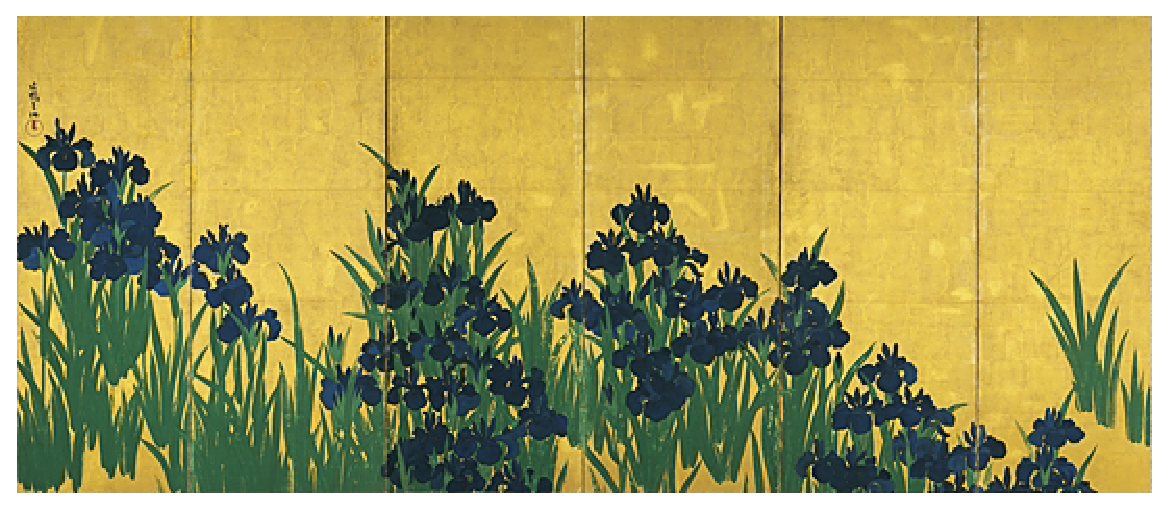
\includegraphics[scale=0.7]{irises_korin.eps}
\end{figure}

\vspace*{2cm}
\begin{flushleft}
{\large The Scalable Software Infrastructure
Project\\
{\tt http://www.ssisc.org/}}\\
\end{flushleft}

\vspace*{5mm}
\thispagestyle{empty}

\newpage
\begin{flushleft}
{\small
Copyright \copyright\ 2005 The Scalable Software Infrastructure Project,
supported by ``Development of Software Infrastructure for Large Scale
Scientific Simulation'' Team, CREST, JST.

Akira Nishida, Research Institute for Information Technology, 
Kyushu University, 6-10-1, Hakozaki, Higashi-ku, Fukuoka 812-8581, Japan.

All rights reserved.

\vspace*{5mm}
 Redistribution and use in source and binary forms, with or without
 modification, are permitted provided that the following conditions are
 met:

 1. Redistributions of source code must retain the above copyright
 notice, this list of conditions and the following disclaimer.

 2. Redistributions in binary form must reproduce the above copyright
 notice, this list of conditions and the following disclaimer in the
 documentation and/or other materials provided with the distribution.

 3. Neither the name of the University nor the names of its contributors
 may be used to endorse or promote products derived from this software
 without specific prior written permission.

\vspace*{5mm}
 THIS SOFTWARE IS PROVIDED BY THE SCALABLE SOFTWARE INFRASTRUCTURE
 PROJECT ``AS IS'' AND ANY EXPRESS OR IMPLIED WARRANTIES, INCLUDING, BUT
 NOT LIMITED TO, THE IMPLIED WARRANTIES OF MERCHANTABILITY AND FITNESS
 FOR A PARTICULAR PURPOSE ARE DISCLAIMED. IN NO EVENT SHALL THE SCALABLE
 SOFTWARE INFRASTRUCTURE PROJECT BE LIABLE FOR ANY DIRECT, INDIRECT,
 INCIDENTAL, SPECIAL, EXEMPLARY, OR CONSEQUENTIAL DAMAGES (INCLUDING,
 BUT NOT LIMITED TO, PROCUREMENT OF SUBSTITUTE GOODS OR SERVICES; LOSS
 OF USE, DATA, OR PROFITS; OR BUSINESS INTERRUPTION) HOWEVER CAUSED AND
 ON ANY THEORY OF LIABILITY, WHETHER IN CONTRACT, STRICT LIABILITY, OR
 TORT (INCLUDING NEGLIGENCE OR OTHERWISE) ARISING IN ANY WAY OUT OF THE
 USE OF THIS SOFTWARE, EVEN IF ADVISED OF THE POSSIBILITY OF SUCH
 DAMAGE.

\vfill
$BI=;f(B: $BHx7A8wNV(B. $B1m;R2V?^(B. 1705$BG/:"(B. $B:,DEH~=Q4[(B.
}
\end{flushleft}
\thispagestyle{empty}

\newpage
\pagenumbering{roman}
\tableofcontents

\setcounter{section}{0}
\pagenumbering{arabic}

\newpage
\section*{$B%P!<%8%g%s(B 1.0 $B$+$i$NJQ99E@(B}
\begin{enumerate}
\item double-double$B7?(B4$BG\@:EY1i;;$KBP1~(B.
\item Fortran$B%3%s%Q%$%i$KBP1~(B.
\item Autotools$B$KBP1~(B.
\item 
\begin{enumerate}
\item $B%=%k%P$N9=B$$rJQ99(B.
\item $B4X?t(B{\tt lis\_matrix\_create()}, {\tt lis\_vector\_create()}$B$N0z?t$rJQ99(B.
\item $B%3%^%s%I%i%$%s%*%W%7%g%s$N5-K!$rJQ99(B.
\end{enumerate}
\end{enumerate}

\section*{$B%P!<%8%g%s(B 1.1 $B$+$i$NJQ99E@(B}
\begin{enumerate}
\item $BI8=`8GM-CMLdBj$KBP1~(B.
\item 64$B%S%C%H@0?t7?$KBP1~(B.
\item 
\begin{enumerate}
\item $B4X?t(B{\tt lis\_output\_residual\_history()}, 
      {\tt lis\_get\_residual\_history()}$B$NL>>N$r$=$l$>$l(B\\
      {\tt lis\_solver\_output\_rhistory()}, {\tt lis\_solver\_get\_rhistory()}$B$KJQ99(B.
\item Fortran$B%$%s%?%U%'!<%9(B{\tt lis\_vector\_set\_value()},
      {\tt lis\_vector\_get\_value()}$B$NG[Ns5/E@$r(B1$B$KJQ99(B.
\item Fortran$B%$%s%?%U%'!<%9(B{\tt lis\_vector\_set\_size()}$B$NG[Ns5/E@$r(B1$B$KJQ99(B.
\item $B1i;;@:EY$K4X$9$k%*%W%7%g%s$NL>>N$r(B{\tt -precision}$B$+$i(B{\tt -f}$B$KJQ99(B.
\end{enumerate}
\item $B4X?t(B{\tt lis\_solve\_kernel()}$B$N;EMM$r(B{\tt lis\_solve\_execute()}$B$G7W;;(B
      $B$5$l$?;D:9$rJV$9$h$&JQ99(B. 
\item $B@0?t7?$N;EMM$rJQ99(B. 
\begin{enumerate}
\item C$B%W%m%0%i%`$K$*$1$k@0?t7?$r(B{\tt LIS\_INT}$B$KJQ99(B. 
      {\tt LIS\_INT}$B$N4{DjCM$O(B{\tt int}. $B%W%j%W%m%;%C%5%^%/%m(B
      {\tt \_LONGLONG}$B$,Dj5A$5$l$?>l9g$K$O(B, {\tt long long int}$B$KCV$-49$($i$l$k(B. 
\item Fortran$B%W%m%0%i%`$K$*$1$k@0?t7?$r(B{\tt LIS\_INTEGER}$B$KJQ99(B. 
      {\tt LIS\_INTEGER}$B$N4{DjCM$O(B{\tt integer}. 
      $B%W%j%W%m%;%C%5%^%/%m(B{\tt LONGLONG}$B$,Dj5A$5$l$?>l9g$K$O(B, 
      {\tt integer*8}$B$KCV$-49$($i$l$k(B. 
\end{enumerate}
\item $B9TNs3JG<7A<0(BCRS (Compressed Row Storage), CCS (Compressed Column Storage)
      $B$NL>>N$r$=$l$>$l(BCSR (Compressed Sparse Row), CSC (Compressed Sparse Column)
      $B$KJQ99(B. 
\item $B4X?t(B{\tt lis\_get\_solvername()}, {\tt lis\_get\_preconname()}, 
      {\tt lis\_get\_esolvername()}$B$NL>>N$r$=$l$>$l(B\\
      {\tt lis\_solver\_get\_solvername()}, 
      {\tt lis\_solver\_get\_preconname()}, 
{\tt lis\_esolver\_get\_esolvername()}$B$KJQ99(B.
\end{enumerate}

\section*{$B%P!<%8%g%s(B 1.2 $B$+$i$NJQ99E@(B}
\begin{enumerate}
\item nmake$B$KBP1~(B.  
\item $B%U%!%$%k(B{\tt lis\_config\_win32.h}$B$NL>>N$r(B{\tt lis\_config\_win.h}
      $B$KJQ99(B.
\item $B9TNs3JG<7A<0(BJDS (Jagged Diagonal Storage)$B$NL>>N$r(BJAD (Jagged Diagonal)
      $B$KJQ99(B. 
\item $B4X?t(B{\tt lis\_fscan\_double()}, {\tt lis\_bswap\_double()}$B$N(B
      $BL>>N$r$=$l$>$l(B{\tt lis\_fscan\_scalar()}, \\
      {\tt lis\_bswap\_scalar()}$B$KJQ99(B.
\end{enumerate}

\section*{$B%P!<%8%g%s(B 1.3 $B$+$i$NJQ99E@(B}
\begin{enumerate}
\item long double$B7?(B4$BG\@:EY1i;;$KBP1~(B.
\item Fortran$B$G$N%]%$%s%?A`:n$KBP1~(B.  
\item $B9=B$BN(B{\tt LIS\_SOLVER}, {\tt LIS\_ESOLVER}$B$N%a%s%P(B{\tt residual}$B$NL>>N$r(B{\tt rhistory}$B$KJQ99(B.
\item $B9=B$BN(B{\tt LIS\_SOLVER}, {\tt LIS\_ESOLVER}$B$N%a%s%P(B{\tt iters}, 
      {\tt iters2}$B$NL>>N$r$=$l$>$l(B{\tt iter}, {\tt iter2}$B$KJQ99(B. 
\item $B4X?t(B{\tt lis\_solver\_get\_iters()}, {\tt lis\_solver\_get\_itersex()}, 
      {\tt lis\_esolver\_get\_iters()}, \\
      {\tt lis\_esolver\_get\_itersex()}$B$NL>>N$r$=$l$>$l(B
      {\tt lis\_solver\_get\_iter()}, {\tt lis\_solver\_get\_iterex()}, 
      {\tt lis\_esolver\_get\_iter()}, {\tt lis\_esolver\_get\_iterex()}$B$KJQ99(B.
\item $B9=B$BN(B{\tt LIS\_SOLVER}, {\tt LIS\_ESOLVER}$B$N%a%s%P(B{\tt *times}$B$NL>>N$r$=$l$>$l(B{\tt *time}$B$KJQ99(B. 
\item $B9=B$BN(B{\tt LIS\_VECTOR}$B$K%a%s%P(B{\tt intvalue}$B$rDI2C(B. 
\item $B4X?t(B{\tt lis\_output\_vector*()}, {\tt lis\_output\_mm\_vec()}$B$N;EMM$r@0?tCM$r3JG<$G$-$k$h$&JQ99(B. 
\item $B4X?t(B{\tt lis\_matrix\_scaling*()}$B$NL>>N$r$=$l$>$l(B
      {\tt lis\_matrix\_scale*()}$B$KJQ99(B.
\item $B4X?t(B{\tt lis\_array\_dot2()}, {\tt lis\_array\_invGauss()}$B$NL>>N$r$=$l$>$l(B
      {\tt lis\_array\_dot()}, {\tt lis\_array\_ge()}$B$KJQ99(B.
\end{enumerate}

\section*{$B%P!<%8%g%s(B 1.4 $B$+$i$NJQ99E@(B}
\begin{enumerate}
\item $BG[NsA`:n$KBP1~(B.
\item $BA0=hM}$H%=%k%P$NJ,N%$KBP1~(B.
\item $B4X?t(B{\tt lis\_array\_qr()}$B$N;EMM$r(BQR$BK!$NH?I|2s?t5Z$S8m:9$rJV$9$h$&JQ99(B. 
\item $B4X?t(B{\tt lis\_array\_matvec2()}, {\tt lis\_array\_matmat2()}$B$NL>>N$r$=$l$>$l(B
  {\tt lis\_array\_matvec\_ns()}, \\
  {\tt lis\_array\_matmat\_ns()}$B$KJQ99(B.
\item $B%W%j%W%m%;%C%5%^%/%m(B{\tt \_LONGLONG}, {\tt LONGLONG}$B$NL>>N$r$=$l$>$l(B
      {\tt \_LONG\_\_LONG}, {\tt LONG\_\_LONG}$B$KJQ99(B.
\end{enumerate}

\section*{$B%P!<%8%g%s(B 1.5 $B$+$i$NJQ99E@(B}
\begin{enumerate}
\item $BJ#AG?t1i;;$KBP1~(B.
\end{enumerate}

\section*{$B%P!<%8%g%s(B 1.6 $B$+$i$NJQ99E@(B}
\begin{enumerate}
\item $B0lHL2=8GM-CMLdBj$KBP1~(B.
\item GCC libquadmath$B$KBP1~(B.  
\item $B8GM-CM2rK!$N%7%U%HNL$NId9f$r47Nc$K9g$o$;$FJQ99(B.
\item {\tt lis\_matrix\_shift\_diagonal()}, {\tt lis\_vector\_shift()}, {\tt lis\_array\_shift()}$B$N%7%U%HNL$NId9f$r$=$l$>$lJQ99(B. 
\end{enumerate}

\section*{$B%P!<%8%g%s(B 1.7 $B$+$i$NJQ99E@(B}
\begin{enumerate}
\item $B%^%k%A%9%F%C%W@~7?J}Dx<02rK!$KBP1~(B.
\item $B%*%W%7%g%s(B{\tt -ssor\_w}$B5Z$S(B{\tt -hybrid\_w}$B$NL>>N$r(B{\tt -ssor\_omega}$B5Z$S(B{\tt -hybrid\_omega}$B$K$=$l$>$lJQ99(B.  
\end{enumerate}

\newpage
\section{$B$O$8$a$K(B}
Lis (Library of Iterative Solvers for linear systems, $BH/2;$O(B[lis])$B$O(B, 
$BJPHyJ,J}Dx<0$N?tCM7W;;$K8=$l$kAB9TNs$r(B
$B78?t$H$9$k@~7?J}Dx<0(B 
\[
Ax = b
\]
$B5Z$S8GM-CMLdBj(B
\[
Ax = \lambda Bx
\]
$B$r2r$/$?$a$NJBNsH?I|K!%=%U%H%&%'%"%i%$%V%i%j$G$"$k(B\cite{nishida1}. 
$BBP1~$9$k@~7?J}Dx<02rK!(B, $B8GM-CM2rK!$N0lMw$rI=(B\ref{tab:solvers}-\ref{tab:esolvers}, 
$BA0=hM}$rI=(B\ref{tab:precon}$B$K<($9(B. 
$B$^$?9TNs3JG<7A<0$N0lMw$rI=(B\ref{tab:storage}$B$K<($9(B. 

\begin{table}[htb]
\begin{minipage}[t]{0.30\textwidth}
\caption{$B@~7?J}Dx<02rK!(B} 
\vspace*{1mm}
\label{tab:solvers}
\hbox to\hsize{\hfil
\begin{tabular}{l|l}\hline\hline
CG\cite{hestenes,lanczos1} & CR\cite{hestenes} \\ 
BiCG\cite{fletcher}     & BiCR\cite{sogabe09} \\
CGS\cite{sonneveld}     & CRS\cite{abe02} \\
BiCGSTAB\cite{bicgstab} & BiCRSTAB\cite{abe02} \\
GPBiCG\cite{zhang}      & GPBiCR\cite{abe02} \\
BiCGSafe\cite{fujino01} & BiCRSafe\cite{fujino02} \\
BiCGSTAB(l)\cite{bicgstabl} & TFQMR\cite{tfqmr} \\
Jacobi\cite{jacobi}     & Orthomin(m)\cite{orthomin} \\
Gauss-Seidel\cite{gauss,seidel} & GMRES(m)\cite{gmres} \\
SOR\cite{young,frankel} & FGMRES(m)\cite{fgmres} \\
IDR(s)\cite{idrs}       & MINRES\cite{minres} \\
COCG\cite{cocg}         & COCR\cite{cocr} \\
\hline         
\end{tabular}
\hfil}
\end{minipage}
\hspace*{13mm}
\begin{minipage}[t]{0.30\textwidth}
\caption{$B8GM-CM2rK!(B} 
\vspace*{1mm}
\label{tab:esolvers}
\hbox to\hsize{\hfil
\begin{tabular}{l}\hline\hline
Power\cite{power} \\
Inverse\cite{inverse} \\
Rayleigh Quotient\cite{rayleigh} \\
CG\cite{knyazev} \\
CR\cite{suetomi} \\
Subspace\cite{rutishauser} \\
Lanczos\cite{lanczos2} \\
Arnoldi\cite{arnoldi} \\
\hline         
\end{tabular}
\hfil}
\end{minipage}
\newline
\begin{minipage}[t]{0.30\textwidth}
\caption{$BA0=hM}(B} 
\vspace*{1mm}
\label{tab:precon}
\hbox to\hsize{\hfil
\begin{tabular}{l}\hline\hline
Jacobi\cite{axelsson} \\
SSOR\cite{axelsson} \\
ILU(k)\cite{gustafsson,nakajima} \\
ILUT\cite{ilut,ITSOL} \\
Crout ILU\cite{ITSOL,iluc} \\
I+S\cite{kohno01} \\
SA-AMG\cite{fujii01}  \\
Hybrid\cite{abe01} \\
SAINV\cite{bridson01}  \\
Additive Schwarz\cite{chan,dryja} \\
$B%f!<%6Dj5A(B \\
\hline         
\end{tabular}
\hfil}
\end{minipage}
\hspace*{-4mm}
\begin{minipage}[t]{0.30\textwidth}
\caption{$B9TNs3JG<7A<0(B} 
\vspace*{1mm}
\label{tab:storage}
\hbox to\hsize{\hfil
\begin{tabular}{ll}\hline\hline
Compressed Sparse Row & (CSR) \\
Compressed Sparse Column & (CSC) \\
Modified Compressed Sparse Row & (MSR) \\
Diagonal &(DIA) \\
Ellpack-Itpack Generalized Diagonal &(ELL) \\
Jagged Diagonal &(JAD) \\
Block Sparse Row & (BSR) \\
Block Sparse Column &(BSC) \\
Variable Block Row &(VBR) \\
Coordinate & (COO) \\
Dense &	(DNS) \\
\hline         
\end{tabular}
\hfil}
\end{minipage}
\end{table}

\newpage
\section{$BF3F~(B}
$BK\@a$G$O(B, $BF3F~(B, $B8!>Z$N<j=g$K$D$$$F=R$Y$k(B. 

\subsection{$B%7%9%F%`MW7o(B}
Lis$B$NF3F~$K$O(BC$B%3%s%Q%$%i$,I,MW$G$"$k(B. 
$B$^$?(B, Fortran$B%$%s%?%U%'!<%9$r;HMQ$9$k>l9g$O(BFortran$B%3%s%Q%$%i(B, 
AMG$BA0=hM}%k!<%A%s$r;HMQ$9$k>l9g$O(BFortran 90$B%3%s%Q%$%i$,I,MW(B
$B$G$"$k(B. $BJBNs7W;;4D6-$G$O(B, OpenMP$B%i%$%V%i%j(B\cite{OpenMP}$B$^$?$O(BMPI-1
$B%i%$%V%i%j(B\cite{MPI}$B$r;HMQ$9$k(B\cite{kota1,kota2}. 
$B%G!<%?$NF~=PNO$K$O(B, Harwell-Boeing 
$B7A<0(B\cite{duff92}, Matrix Market$B7A<0(B\cite{matrixmarket}$B$,MxMQ2DG=$G$"$k(B. 
$BI=(B\ref{platforms}$B$K<g$JF0:n3NG'4D6-$r<($9(B
 ($BI=(B\ref{targetoption}$B$b;2>H$N$3$H(B). 

\begin{table}[htbp]
\caption{$B<g$JF0:n3NG'4D6-(B}
\label{platforms}
\begin{center}
{\small
 \begin{tabular}{l|l}
\hline
\multicolumn{1}{c|}{C$B%3%s%Q%$%i(B ($BI,?\(B) } & \multicolumn{1}{c}{OS} \\
\hline
Intel C/C++ Compiler 7.0, 8.0, 9.1, 10.1, 11.1, 12.1, 14.0, 16.0, 17.0 & Linux \\
                                                     & Windows  \\
\hline
IBM XL C/C++ V7.0, 9.0                     & AIX   \\
                                           & Linux \\
\hline
Sun WorkShop 6, Sun ONE Studio 7,          & Solaris \\
Sun Studio 11, 12                          &         \\
\hline
PGI C++ 6.0, 7.1, 10.5, 16.10              & Linux \\
\hline
gcc 3.3, 4.4, 5.4                          & Linux \\
                                           & Mac OS X \\
                                           & Windows \\
\hline
Microsoft Visual C++ 2008, 2010, 2012, 2013, 2015, 2017       & Windows \\
\hline
\hline
\multicolumn{1}{c|}{Fortran$B%3%s%Q%$%i(B ($B%*%W%7%g%s(B) } & \multicolumn{1}{c}{OS} \\
\hline
Intel Fortran Compiler 8.1, 9.1, 10.1, 11.1, 12.1, 14.0, 16.0, 17.0 & Linux \\
                                                  & Windows  \\
\hline
IBM XL Fortran V9.1, 11.1                  & AIX     \\
                                           & Linux   \\
\hline
Sun WorkShop 6, Sun ONE Studio 7,          & Solaris \\
Sun Studio 11, 12                          &         \\
\hline
PGI Fortran 6.0, 7.1, 10.5, 16.10          & Linux \\
\hline
g77 3.3                                    & Linux \\
gfortran 4.4, 5.4                          & Mac OS X \\
                                           & Windows \\
\hline
\end{tabular}
}
\end{center}
\end{table} 

\subsection{UNIX$B5Z$S8_49%7%9%F%`$X$NF3F~(B}
\subsubsection{$B%"!<%+%$%V$NE83+(B}
$B<!$N%3%^%s%I$rF~NO$7(B, $B%"!<%+%$%V$rE83+$9$k(B. \verb|($VERSION)|$B$O%P!<%8%g%s$r<($9(B. \\
\verb&      > gunzip -c lis-($VERSION).tar.gz | tar xvf - &\\
$B$3$l$K$h$j(B, $B%G%#%l%/%H%j(B{\tt lis-(\$VERSION)}$B$K(B
$B?^(B\ref{listargz}$B$K<($9%5%V%G%#%l%/%H%j$,:n@.$5$l$k(B. 

\begin{figure}[htbp]
\begin{center}
\begin{verbatim}
lis-($VERSION)
 + config
 |  $B@_Dj%U%!%$%k(B
 + doc
 |  $B@bL@=q(B
 + graphics
 |  $BIA2hMQ%5%s%W%k%U%!%$%k(B
 + include
 |  $B%X%C%@%U%!%$%k(B
 + src
 |  $B%=!<%9%U%!%$%k(B
 + test
 |  $B8!>Z%W%m%0%i%`(B
 + win
    Windows$B%7%9%F%`MQ@_Dj%U%!%$%k(B
\end{verbatim}
\end{center}
\caption{{\tt lis-(\$VERSION).tar.gz}$B$N%U%!%$%k9=@.(B}
\label{listargz}
\end{figure}

\subsubsection{$B%=!<%9%D%j!<$N@_Dj(B}
$B%G%#%l%/%H%j(B{\tt lis-(\$VERSION)}$B$K$*$$$F<!$N%3%^%s%I$r<B9T$7(B, $B%=!<%9%D%j!<$r@_Dj$9$k(B. 
\begin{itemize}
\item $B4{Dj$N@_Dj$r;HMQ$9$k>l9g(B : \verb&      > ./configure&
\item $BF3F~@h$r;XDj$9$k>l9g(B :   \verb&      > ./configure --prefix=<install-dir>&
\end{itemize}
$BI=(B\ref{configoption}$B$K<g$J@_Dj%*%W%7%g%s$r<($9(B. 
$B$^$?(B, $BI=(B\ref{targetoption}$B$K(B\verb+TARGET+$B$H$7$F;XDj$G$-$k<g$J7W;;5!4D6-$r<($9(B. 
\begin{table}[htbp]
\caption{$B<g$J@_Dj%*%W%7%g%s(B ($B0lMw$O(B {\tt ./configure --help}$B$r;2>H(B) }
\label{configoption}
\begin{center}
\begin{tabular}{|l|l|}
\hline
\verb+--enable-omp+      & OpenMP$B%i%$%V%i%j$r;HMQ(B\\ \hline
\verb+--enable-mpi+      & MPI$B%i%$%V%i%j$r;HMQ(B\\ \hline
\verb+--enable-fortran+  & FORTRAN 77$B8_49%$%s%?%U%'!<%9$r;HMQ(B\\ \hline
\verb+--enable-f90    +  & Fortran 90$B8_49%$%s%?%U%'!<%9$r;HMQ(B\\ \hline
\verb+--enable-saamg+    & SA-AMG$BA0=hM}$r;HMQ(B\\ \hline
\verb+--enable-quad+     & double-double$B7?(B4$BG\@:EY1i;;$r;HMQ(B\\ \hline
\verb+--enable-longdouble+ & long double$B7?(B4$BG\@:EY1i;;$r;HMQ(B\\ \hline
\verb+--enable-longlong+ & 64$B%S%C%H@0?t7?$r;HMQ(B\\ \hline
\verb+--enable-complex+  & $B%9%+%i7?$H$7$FJ#AG?t7?$r;HMQ(B\\ \hline
\verb+--enable-debug+    & $B%G%P%C%0%b!<%I$r;HMQ(B\\ \hline
\verb+--enable-shared+   & $BF0E*%j%s%/$r;HMQ(B\\ \hline
\verb+--enable-gprof+    & $B%W%m%U%!%$%i$r;HMQ(B\\ \hline
\verb+--prefix=<install-dir>+    & $BF3F~@h$r;XDj(B\\ \hline
\verb+TARGET=<target>+    & $B7W;;5!4D6-$r;XDj(B\\ \hline
\verb+CC=<c_compiler>+    & C$B%3%s%Q%$%i$r;XDj(B\\ \hline
\verb+CFLAGS=<c_flags>+    & C$B%3%s%Q%$%i%*%W%7%g%s$r;XDj(B\\ \hline
\verb+F77=<f77_compiler>+    & FORTRAN 77$B%3%s%Q%$%i$r;XDj(B\\ \hline
\verb+F77FLAGS=<f77_flags>+    & FORTRAN 77$B%3%s%Q%$%i%*%W%7%g%s$r;XDj(B\\ \hline
\verb+FC=<f90_compiler>+    & Fortran 90$B%3%s%Q%$%i$r;XDj(B\\ \hline
\verb+FCFLAGS=<f90_flags>+    & Fortran 90$B%3%s%Q%$%i%*%W%7%g%s$r;XDj(B\\ \hline
\verb+LDFLAGS=<ld_flags>+    & $B%j%s%/%*%W%7%g%s$r;XDj(B\\ \hline
\end{tabular}
\end{center}
\end{table}
\begin{table}[htbp]
\caption{TARGET$B$NNc(B ($B>\:Y$O(B{\tt lis-(\$VERSION)/configure.ac}$B$r;2>H(B) }
\label{targetoption}
\begin{center}
\begin{tabular}{|l|l|}
\hline
\verb+<target>+           & $BEy2A$J%*%W%7%g%s(B \\ \hline
\verb+cray_xt3_cross+     & \verb+./configure CC=cc FC=ftn CFLAGS="-O3 -B -fastsse -tp k8-64"+ \\
                          & \verb+  FCFLAGS="-O3 -fastsse -tp k8-64 -Mpreprocess" FCLDFLAGS="-Mnomain"+\\
                          & \verb+  ac_cv_sizeof_void_p=8 cross_compiling=yes+\\
                          & \verb+  ax_f77_mangling="lower case, no underscore, extra underscore"+ \\ \hline
\verb+fujitsu_fx10_cross+ & \verb|./configure CC=fccpx FC=frtpx CFLAGS="-Kfast,ocl,preex"| \\
                          & \verb+  FCFLAGS="-Kfast,ocl,preex -Cpp -fs" FCLDFLAGS="-mlcmain=main"+\\
                          & \verb+  ac_cv_sizeof_void_p=8 cross_compiling=yes+\\
                          & \verb+  ax_f77_mangling="lower case, underscore, no extra underscore"+ \\ \hline
\verb+hitachi_sr16k+      & \verb|./configure CC=cc FC=f90 CFLAGS="-Os -noparallel"| \\
                          & \verb+  FCFLAGS="-Oss -noparallel" FCLDFLAGS="-lf90s"+ \\
                          & \verb+  ac_cv_sizeof_void_p=8+ \\
                          & \verb+  ax_f77_mangling="lower case, underscore, no extra underscore" + \\ \hline
\verb+ibm_bgl_cross+      & \verb+./configure CC=blrts_xlc FC=blrts_xlf90+ \\
                          & \verb+  CFLAGS="-O3 -qarch=440d -qtune=440 -qstrict"+ \\
                          & \verb+  FCFLAGS="-O3 -qarch=440d -qtune=440 -qsuffix=cpp=F90"+ \\
                          & \verb+  ac_cv_sizeof_void_p=4 cross_compiling=yes+\\
                          & \verb+  ax_f77_mangling="lower case, no underscore, no extra underscore"+ \\ \hline
\verb+intel_mic_cross+    & \verb+./configure CC=icc F77=ifort FC=ifort+ \\
                          & \verb+  MPICC=mpiicc MPIF77=mpiifort MPIFC=mpiifort+ \\
                          & \verb+  CFLAGS="-mmic" FFLAGS="-mmic" FCFLAGS="-mmic"+ \\
                          & \verb+  LDFLAGS="-mmic" FCLDFLAGS="-mmic" cross_compiling=yes+ \\
                          & \verb+  host=x86_64-pc-linux-gnu host_alias=x86_64-linux-gnu+ \\
                          & \verb+  host_cpu=x86_64 host_os=linux-gnu host_vendor=pc+ \\
                          & \verb+  target=k1om-mpss-linux-gnu target_alias=k1om-mpss-linux+ \\
                          & \verb+  target_cpu=k1om target_os=linux-gnu target_vendor=mpss+ \\ \hline
\verb+nec_sx9_cross+      & \verb|./configure CC=sxmpic++ FC=sxmpif90 AR=sxar RANLIB=true | \\
                          & \verb+  ac_cv_sizeof_void_p=8 ax_vector_machine=yes cross_compiling=yes+ \\ 
                          & \verb+  ax_f77_mangling="lower case, no underscore, extra underscore"+ \\ \hline
\end{tabular}
\end{center}
\end{table}

\subsubsection{$B<B9T%U%!%$%k$N@8@.(B}
$B%G%#%l%/%H%j(B{\tt lis-(\$VERSION)}$B$K$*$$$F<!$N%3%^%s%I$rF~NO$7(B, $B<B9T%U%!%$%k$r@8@.$9$k(B.\\
 \verb+      > make +\\
$B<B9T%U%!%$%k$,@5>o$K@8@.$5$l$?$+$I$&$+$r3NG'$9$k$K$O(B, 
$B%G%#%l%/%H%j(B{\tt lis-(\$VERSION)}$B$K$*$$$F<!$N%3%^%s%I$rF~NO$7(B, $B%G%#%l%/(B
 $B%H%j(B{\tt lis-(\$VERSION)/test}$B$K@8@.$5$l$?<B9T%U%!%$%k$rMQ$$$F8!>Z$r9T$&(B. \\
 \verb+      > make check+\\
$B$3$N%3%^%s%I$G$O(B, Matrix Market$B7A<0$N%U%!%$%k(B{\tt test/testmat.mtx}
$B$+$i9TNs(B, $B%Y%/%H%k%G!<%?$rFI$_9~$_(B, BiCG$BK!$rMQ$$$F@~7?J}Dx<0(B$Ax=b$$B$N2r$r(B
$B5a$a$k(B. $B0J2<$K(BSGI Altix 3700$B>e$G$N<B9T7k2L$r<($9(B. 
$B$J$*%*%W%7%g%s(B{\tt --enable-omp}$B$H(B{\tt --enable-mpi}$B$OAH$_9g$o$;$F(B
$B;HMQ$9$k$3$H$,$G$-$k(B. 
\begin{itembox}[l]{$B4{Dj(B}
\begin{minipage}{10cm}
\begin{verbatim}
matrix size = 100 x 100 (460 nonzero entries)

initial vector x      : 0
precision             : double
linear solver         : BiCG
preconditioner        : none
convergence condition : ||b-Ax||_2 <= 1.0e-12 * ||b-Ax_0||_2
matrix storage format : CSR
linear solver status  : normal end

BiCG: number of iterations = 15 (double = 15, quad = 0)
BiCG: elapsed time         = 5.178690e-03 sec.
BiCG:   preconditioner     = 1.277685e-03 sec.
BiCG:     matrix creation  = 1.254797e-03 sec.
BiCG:   linear solver      = 3.901005e-03 sec.
BiCG: relative residual    = 6.327297e-15
\end{verbatim}
\end{minipage}
\end{itembox}
\begin{itembox}[l]{{\tt --enable-omp}}
 \begin{minipage}{10cm}
 \begin{verbatim}
max number of threads = 32
number of threads = 2
matrix size = 100 x 100 (460 nonzero entries)

initial vector x      : 0
precision             : double
linear solver         : BiCG
preconditioner        : none
convergence condition : ||b-Ax||_2 <= 1.0e-12 * ||b-Ax_0||_2
matrix storage format : CSR
linear solver status  : normal end

BiCG: number of iterations = 15 (double = 15, quad = 0)
BiCG: elapsed time         = 8.960009e-03 sec.
BiCG:   preconditioner     = 2.297878e-03 sec.
BiCG:     matrix creation  = 2.072096e-03 sec.
BiCG:   linear solver      = 6.662130e-03 sec.
BiCG: relative residual    = 6.221213e-15
\end{verbatim}
\end{minipage}
\end{itembox}
\begin{itembox}[l]{\tt --enable-mpi}
 \begin{minipage}{10cm}
 \begin{verbatim}
number of processes = 2
matrix size = 100 x 100 (460 nonzero entries)

initial vector x      : 0
precision             : double
linear solver         : BiCG
preconditioner        : none
convergence condition : ||b-Ax||_2 <= 1.0e-12 * ||b-Ax_0||_2
matrix storage format : CSR
linear solver status  : normal end

BiCG: number of iterations = 15 (double = 15, quad = 0)
BiCG: elapsed time         = 2.911400e-03 sec.
BiCG:   preconditioner     = 1.560780e-04 sec.
BiCG:     matrix creation  = 1.459997e-04 sec.
BiCG:   linear solver      = 2.755322e-03 sec.
BiCG: relative residual    = 6.221213e-15
\end{verbatim}
\end{minipage}
\end{itembox}

\subsubsection{$BF3F~(B}
$B%G%#%l%/%H%j(B{\tt lis-(\$VERSION)}$B$K$*$$$F<!$N%3%^%s%I$rF~NO$7(B, $BF3F~@h$N%G%#%l%/%H%j$K%U%!%$%k$rJ#@=$9$k(B.\\
 \verb+      > make install+\\ 
$B$3$l$K$h$j(B, $B%G%#%l%/%H%j(B{\tt (\$INSTALLDIR)}$B$K0J2<$N%U%!%$%k$,J#@=$5$l$k(B.

\begin{verbatim}
($INSTALLDIR)
 +bin
 |   +lsolve esolve gesolve hpcg_kernel hpcg_spmvtest spmvtest*
 +include
 |   +lis_config.h lis.h lisf.h
 +lib
 |   +liblis.a
 +share
     +doc/lis examples/lis man
\end{verbatim}
{\tt lis\_config.h}$B$O%i%$%V%i%j$r@8@.$9$k:]$K(B, $B$^$?(B{\tt lis.h}$B$O(BC, {\tt lisf.h}$B$O(BFortran$B$G(B
$B%i%$%V%i%j$r;HMQ$9$k:]$KI,MW$J%X%C%@%U%!%$%k$G$"$k(B. {\tt liblis.a}$B$O@8@.$5$l$?(B
$B%i%$%V%i%j$G$"$k(B. 
$B%i%$%V%i%j$,@5>o$KF3F~$5$l$?$+$I$&$+$r3NG'$9$k$K$O(B, 
$B%G%#%l%/%H%j(B{\tt lis-(\$VERSION)}$B$K$*$$$F<!$N%3%^%s%I$rF~NO$7(B, $B%G%#%l%/(B
$B%H%j(B{\tt examples/lis}$B$K@8@.$5$l$?<B9T%U%!%$%k$rMQ$$$F8!>Z$r9T$&(B. \\
 \verb+      > make installcheck+ \\
{\tt examples/lis}$B2<$N(B{\tt test1}, {\tt etest5}, {\tt getest5}, 
{{\tt test3b}, {{\tt spmvtest3b}$B$O(B, 
{\tt lsolve}, {\tt esolve}, {\tt gesolve},\\ 
{\tt hpcg\_kernel}, {\tt hpcg\_spmvtest}$B$NJLL>$G(B{\tt (\$INSTALLDIR)/bin}$B$KJ#@=$5$l$k(B.
{\tt examples/lis/spmvtest*}$B$b(B, $B$=$l$>$l(B{\tt (\$INSTALLDIR)/bin}$B$K(B
$BJ#@=$5$l$k(B.

{\tt (\$INSTALLDIR)}$B$KJ#@=$5$l$?%U%!%$%k$r:o=|$9$k$K$O!$(B
$B<!$N%3%^%s%I$rF~NO$9$k(B. \\
 \verb+      > make uninstall+\\
{\tt lis-(\$VERSION)}$B$K@8@.$5$l$?%i%$%V%i%j(B, $B5Z$S<B9T%U%!%$%k$r:o=|$9$k$K$O!$(B
$B<!$N%3%^%s%I$rF~NO$9$k(B. \\
 \verb+      > make clean+\\
$B@8@.$5$l$?@_Dj%U%!%$%k$r9g$o$;$F:o=|$9$k$K$O!$(B
$B<!$N%3%^%s%I$rF~NO$9$k(B. \\
 \verb+      > make distclean+

\subsection{Windows$B%7%9%F%`$X$NF3F~(B}
$BE,Ev$J%D!<%k$rMQ$$$F%"!<%+%$%V$rE83+$7$?8e(B, 
Microsoft Build Engine$B$r;HMQ$9$k>l9g$O(B, 
$B%G%#%l%/%H%j(B{\tt lis-(\$VERSION)\textbackslash win}$B$K$*$$$F<!$N%3%^%s%I$rF~NO$7(B, 
$B@_Dj%U%!%$%k(B{\tt Makefile}$B$r@8@.$9$k(B 
($B>\:Y$O(B{\tt configure.bat --help}$B$r;2>H(B). \\
 \verb+      > configure.bat+\\
{\tt Makefile}$B$N4{DjCM$O(B{\tt Makefile.in}$B$GDj5A$5$l$k(B. 
$B<B9T%U%!%$%k$r@8@.$9$k$K$O(B, {\tt lis-(\$VERSION)\textbackslash win}
$B$K$*$$$F<!$N%3%^%s%I$rF~NO$9$k(B. \\
 \verb+      > nmake+\\
$B<B9T%U%!%$%k$,@5>o$K@8@.$5$l$?$+$I$&$+$r3NG'$9$k$K$O(B, 
$B<!$N%3%^%s%I$rF~NO$7(B, $B@8@.$5$l$?<B9T%U%!%$%k$rMQ$$$F8!>Z$r9T$&(B. \\
 \verb+      > nmake check+\\
$B@8@.$5$l$?%i%$%V%i%j(B, $B<B9T%U%!%$%k(B, $B%X%C%@%U%!%$%k(B, $B5Z$S(BPDF$BJ8=q$O(B,
$B0J2<$N%3%^%s%I$K$h$j(B\\
{\tt (\$INSTALLDIR)\textbackslash lib}, 
{\tt (\$INSTALLDIR)\textbackslash bin},
{\tt (\$INSTALLDIR)\textbackslash include}, 
$B5Z$S(B{\tt (\$INSTALLDIR)\textbackslash doc}
$B$K$=$l$>$l3JG<$5$l$k(B. \\
 \verb+      > nmake install+\\
{\tt (\$INSTALLDIR)}$B$KJ#@=$5$l$?%U%!%$%k$r:o=|$9$k$K$O!$(B
$B<!$N%3%^%s%I$rF~NO$9$k(B. \\
 \verb+      > nmake uninstall+\\
{\tt (\$INSTALLDIR)\textbackslash win}$B$K@8@.$5$l$?%i%$%V%i%j(B,
$B5Z$S<B9T%U%!%$%k$r:o=|$9$k$K$O!$<!$N%3%^%s%I$rF~NO$9$k(B. \\
 \verb+      > nmake clean+\\
$B@8@.$5$l$?@_Dj%U%!%$%k$r9g$o$;$F:o=|$9$k$K$O!$<!$N%3%^%s%I$rF~NO$9$k(B. \\
 \verb+      > nmake distclean+

UNIX$B8_494D6-$r;HMQ$9$k>l9g$OA0@a$r;2>H$N$3$H(B. 

\subsection{$B8!>Z(B}
$B8!>Z%W%m%0%i%`$O(B{\tt lis-(\$VERSION)/test}$B$K3JG<$5$l$k(B. 
\subsubsection{test1}
$B%G%#%l%/%H%j(B{\tt lis-(\$VERSION)/test}$B$K$*$$$F(B\\
 \verb+      > test1 matrix_filename rhs_setting solution_filename rhistory_filename [options]+\\
$B$HF~NO$9$k$H(B, {\tt matrix\_filename}$B$+$i9TNs%G!<%?$rFI$_9~$_(B, 
$B@~7?J}Dx<0(B$Ax=b$$B$r(B{\tt options}$B$G;XDj$5$l$?2rK!$G2r$/(B. $B$^$?(B, 
$B2r$r3HD%(BMatrix Market$B7A<0$G(B{\tt solution\_filename}$B$K(B, 
$B;D:9MzNr$r(BPLAIN$B7A<0$G(B{\tt rhistory\_filename}$B$K=q$-=P$9(B 
($BIUO?(B\ref{sec:matinp}$B$r;2>H(B). 
$BF~NO2DG=$J9TNs%G!<%?7A<0$O3HD%(BMatrix Market$B7A<0(B, Harwell-Boeing$B7A<0$N$$$:$l$+$G$"$k(B. 
{\tt rhs\_setting}$B$K$O(B
\begin{namelist}{XXXXXXXXXXXXXXXXXXXX}
\item[0] $B9TNs%G!<%?%U%!%$%k$K4^$^$l$k1&JU%Y%/%H%k$rMQ$$$k(B
\item[1] $b = (1,\dots,1)^T$$B$rMQ$$$k(B
\item[2] $b = A \times (1,\dots,1)^T$$B$rMQ$$$k(B
\item[rhs\_filename] $B1&JU%Y%/%H%k$N%U%!%$%kL>(B
\end{namelist}
$B$N$$$:$l$+$r;XDj$G$-$k(B. {\tt rhs\_filename}$B$O(BPLAIN$B7A<0(B, Matrix Market$B7A<0$KBP1~$9$k(B. 
{\tt test1f.F}$B$O(B{\tt test1.c}$B$N(BFortran$BHG$G$"$k(B. 

\subsubsection{test2}
$B%G%#%l%/%H%j(B{\tt lis-(\$VERSION)/test}$B$K$*$$$F(B\\
 \verb+      > test2 m n matrix_type solution_filename rhistory_filename [options]+\\
$B$HF~NO$9$k$H(B, 2$B<!85(BLaplace$B:nMQAG$r(B5$BE@Cf?4:9J,$K$h$jN%;62=$7$FF@$i$l$k(B
$B<!?t(B$mn$$B$N9TNs(B$A$$B$r78?t$H$9$k(B
$B@~7?J}Dx<0(B$Ax=b$$B$r(B, \verb|matrix_type|$B$G;XDj$5$l$?9TNs3JG<7A<0(B, 
{\tt options}$B$G;XDj$5$l$?2rK!$G2r$/(B. $B$^$?(B, 
$B2r$r3HD%(BMatrix Market$B7A<0$G(B{\tt solution\_filename}$B$K(B, 
$B;D:9MzNr$r(BPLAIN$B7A<0$G(B{\tt rhistory\_filename}$B$K=q$-=P$9(B.
$B1&JU%Y%/%H%k(B$b$$B$O2r%Y%/%H%k(B$x$$B$NCM$,(B
$B$9$Y$F(B$1$$B$H$J$k$h$&@_Dj$5$l$k(B. {\tt m}, {\tt n}$B$O3F<!85$N3J;RE@?t$G$"$k(B. 
{\tt test2f.F90}$B$O(B{\tt test2.c}$B$N(BFortran 90$BHG$G$"$k(B. 

\subsubsection{test2b}
$B%G%#%l%/%H%j(B{\tt lis-(\$VERSION)/test}$B$K$*$$$F(B\\
 \verb+      > test2b m n matrix_type solution_filename rhistory_filename [options]+\\
$B$HF~NO$9$k$H(B, 2$B<!85(BLaplace$B:nMQAG$r(B9$BE@Cf?4:9J,$K$h$jN%;62=$7$FF@$i$l$k(B
$B<!?t(B$mn$$B$N9TNs(B$A$$B$r78?t$H$9$k(B
$B@~7?J}Dx<0(B$Ax=b$$B$r(B, \verb|matrix_type|$B$G;XDj$5$l$?9TNs3JG<7A<0(B, 
{\tt options}$B$G;XDj$5$l$?2rK!$G2r$/(B. $B$^$?(B, 
$B2r$r3HD%(BMatrix Market$B7A<0$G(B{\tt solution\_filename}$B$K(B, 
$B;D:9MzNr$r(BPLAIN$B7A<0$G(B{\tt rhistory\_filename}$B$K=q$-=P$9(B.
$B1&JU%Y%/%H%k(B$b$$B$O2r%Y%/%H%k(B$x$$B$NCM$,$9$Y$F(B$1$$B$H$J$k$h$&@_Dj$5$l$k(B. {\tt m}, {\tt n}$B$O3F<!85$N3J;RE@?t$G$"$k(B. 

\subsubsection{test3}
$B%G%#%l%/%H%j(B{\tt lis-(\$VERSION)/test}$B$K$*$$$F(B\\
 \verb+      > test3 l m n matrix_type solution_filename rhistory_filename [options]+\\
$B$HF~NO$9$k$H(B, 3$B<!85(BLaplace$B:nMQAG$r(B7$BE@Cf?4:9J,$K$h$jN%;62=$7$FF@$i$l$k(B
$B<!?t(B$lmn$$B$N9TNs(B$A$$B$r78?t$H$9$k(B
$B@~7?J}Dx<0(B$Ax=b$$B$r(B, \verb|matrix_type|$B$G;XDj$5$l$?9TNs3JG<7A<0(B, 
{\tt options}$B$G;XDj$5$l$?2rK!$G2r$/(B. $B$^$?(B, 
$B2r$r3HD%(BMatrix Market$B7A<0$G(B{\tt solution\_filename}$B$K(B, 
$B;D:9MzNr$r(BPLAIN$B7A<0$G(B{\tt rhistory\_filename}$B$K=q$-=P$9(B.
$B1&JU%Y%/%H%k(B$b$$B$O2r%Y%/%H%k(B$x$$B$NCM$,$9$Y$F(B$1$$B$H$J$k$h$&(B
$B@_Dj$5$l$k(B. {\tt l}, {\tt m}, {\tt n}$B$O3F<!85$N3J;RE@?t$G$"$k(B. 

\subsubsection{test3b}
$B%G%#%l%/%H%j(B{\tt lis-(\$VERSION)/test}$B$K$*$$$F(B\\
 \verb+      > test3b l m n matrix_type solution_filename rhistory_filename [options]+\\
$B$HF~NO$9$k$H(B, 3$B<!85(BLaplace$B:nMQAG$r(B27$BE@Cf?4:9J,$K$h$jN%;62=$7$FF@$i$l$k(B
$B<!?t(B$lmn$$B$N9TNs(B$A$$B$r78?t$H$9$k(B
$B@~7?J}Dx<0(B$Ax=b$$B$r(B, \verb|matrix_type|$B$G;XDj$5$l$?9TNs3JG<7A<0(B, 
{\tt options}$B$G;XDj$5$l$?2rK!$G2r$/(B. $B$^$?(B, 
$B2r$r3HD%(BMatrix Market$B7A<0$G(B{\tt solution\_filename}$B$K(B, 
$B;D:9MzNr$r(BPLAIN$B7A<0$G(B{\tt rhistory\_filename}$B$K=q$-=P$9(B.
$B1&JU%Y%/%H%k(B$b$$B$O2r%Y%/%H%k(B$x$$B$NCM$,$9$Y$F(B$1$$B$H$J$k$h$&(B
$B@_Dj$5$l$k(B. {\tt l}, {\tt m}, {\tt n}$B$O3F<!85$N3J;RE@?t$G$"$k(B. 

\subsubsection{test3c}
$B%G%#%l%/%H%j(B{\tt lis-(\$VERSION)/test}$B$K$*$$$F(B\\
 \verb+      > test3c l m n step [options]+\\
$B$HF~NO$9$k$H(B, 3$B<!85(BLaplace$B:nMQAG$r(B7$BE@Cf?4:9J,$K$h$jN%;62=$7$FF@$i$l$k(B
$B<!?t(B$lmn$$B$N9TNs(B$A$$B$r78?t$H$9$k(B
$B@~7?J}Dx<0(B$Ax=b$$B$r(B, {\tt options}$B$G;XDj$5$l$?2rK!$G(B{\tt step}$B%9%F%C%WJ,2r$/(B.
$B1&JU%Y%/%H%k(B$b$$B$O2r%Y%/%H%k(B$x$$B$NCM$,$9$Y$F(B$1$$B$H$J$k$h$&(B
$B@_Dj$5$l$k(B. $B9TNs!$1&JU%Y%/%H%k$NCM$O%9%F%C%WKh$K99?7$5$l$k!%(B
{\tt l}, {\tt m}, {\tt n}$B$O3F<!85$N3J;RE@?t$G$"$k(B. 
$B!!(B
\subsubsection{test4}
$B@~7?J}Dx<0(B$Ax=b$$B$r;XDj$5$l$?2rK!$G2r$-(B, $B2r$rI8=`=PNO$K=q$-=P$9(B. 
$B9TNs(B$A$$B$O<!?t(B$12$$B$N(B3$B=EBP3Q9TNs(B
\[
A = 
\left(
\begin{array}{ccccc}
2 & -1 &   &  &   \\
-1 & 2 & -1 &  &   \\
  & \ddots  & \ddots  & \ddots  &   \\
  &   & -1 & 2 & -1 \\
  &   &   & -1 & 2 \\
\end{array}
\right)
\]
$B$G$"$k(B. $B1&JU%Y%/%H%k(B$b$$B$O2r%Y%/%H%k(B$x$$B$NCM$,$9$Y$F(B$1$$B$H$J$k$h$&(B
$B@_Dj$5$l$k(B. 
{\tt test4f.F}$B$O(B{\tt test4.c}$B$N(BFortran$BHG$G$"$k(B. 

\subsubsection{test5}
$B%G%#%l%/%H%j(B{\tt lis-(\$VERSION)/test}$B$K$*$$$F(B\\
 \verb+      > test5 n gamma [options]+\\
$B$HF~NO$9$k$H(B, 
$B@~7?J}Dx<0(B$Ax=b$$B$r;XDj$5$l$?2rK!$G2r$/(B. 
$B9TNs(B$A$$B$O<!?t(B$n$$B$N(BToepliz$B9TNs(B
\[
A = \left(
\begin{array}{cccccc}
2 & 1 &   &  &  & \\
0 & 2 & 1 &  &  & \\
\gamma & 0& 2 & 1 &  & \\
 & \ddots & \ddots & \ddots & \ddots & \\
 &  &   \gamma &0 &       2   & 1 \\
 &  &  &   \gamma & 0& 2 \\
\end{array}
\right)
\]
$B$G$"$k(B. $B1&JU%Y%/%H%k(B$b$$B$O2r%Y%/%H%k(B$x$$B$NCM$,$9$Y$F(B$1$$B$H$J$k$h$&(B
$B@_Dj$5$l$k(B. 

\subsubsection{test6}
{\tt test6.c}$B$O(B{\tt test2.c}$B$NG[NsHG$G$"$k(B. 
$B%G%#%l%/%H%j(B{\tt lis-(\$VERSION)/test}$B$K$*$$$F(B\\
 \verb+      > test6 m n+\\
$B$HF~NO$9$k$H(B, 2$B<!85(BLaplace$B:nMQAG$r(B5$BE@Cf?4:9J,$K$h$jN%;62=$7$FF@$i$l$k(B
$B<!?t(B$mn$$B$N9TNs(B$A$$B$r78?t$H$9$k@~7?J}Dx<0(B$Ax=b$$B$rD>@\K!$G2r$/(B.
$B1&JU%Y%/%H%k(B$b$$B$O2r%Y%/%H%k(B$x$$B$NCM$,(B
$B$9$Y$F(B$1$$B$H$J$k$h$&@_Dj$5$l$k(B. {\tt m}, {\tt n}$B$O3F<!85$N3J;RE@?t$G$"$k(B. 
{\tt test6f.F90}$B$O(B{\tt test6.c}$B$N(BFortran 90$BHG$G$"$k(B.

\subsubsection{test7}
$B%G%#%l%/%H%j(B{\tt lis-(\$VERSION)/test}$B$K$*$$$F(B\\
 \verb+      > test7+\\
$B$HF~NO$9$k$H(B, $BJ#AG1i;;$N;HMQNc$r<($9(B.
{\tt test7f.F}$B$O(B{\tt test7.c}$B$N(BFortran$BHG$G$"$k(B.

\subsubsection{etest1}
$B%G%#%l%/%H%j(B{\tt lis-(\$VERSION)/test}$B$K$*$$$F(B\\
 \verb+      > etest1 matrix_filename evector_filename rhistory_filename [options]+\\
$B$HF~NO$9$k$H(B, {\tt matrix\_filename}$B$+$i9TNs%G!<%?$rFI$_9~$_(B, 
$BI8=`8GM-CMLdBj(B$Ax=\lambda x$$B$r(B{\tt options}$B$G;XDj$5$l$?2rK!$G2r$$$F(B, $B;XDj$5$l(B
$B$?8GM-CM$rI8=`=PNO$K=q$-=P$9(B. $B$^$?(B, $BBP1~$9$k8GM-%Y%/%H%k$r3HD%(BMatrix
 Market$B7A<0$G(B{\tt evector\_filename}$B$K(B, $B;D:9MzNr$r(BPLAIN$B7A<0$G(B
{\tt rhistory\_filename}$B$K=q$-=P$9(B. 
$BF~NO2DG=$J9TNs%G!<%?7A<0$O(BMatrix Market$B7A<0(B, $B$b$7$/$O(BHarwell-Boeing$B7A<0$N(B
$B$$$:$l$+$G$"$k(B. 
{\tt etest1f.F}$B$O(B{\tt etest1.c}$B$N(BFortran$BHG$G$"$k(B. 
$BJ#?t$N8GM-BP$r<hF@$9$k>l9g$O(B{\tt etest5}$B$r;2>H$N$3$H(B.

\subsubsection{getest1}
$B%G%#%l%/%H%j(B{\tt lis-(\$VERSION)/test}$B$K$*$$$F(B\\
 \verb+      > getest1 matrix_a_filename matrix_b_filename evector_filename rhistory_filename +\\
\verb+ [options]+\\
$B$HF~NO$9$k$H(B, {\tt matrix\_a\_filename}$B5Z$S(B{\tt matrix\_b\_filename}$B$+$i(B
$B9TNs%G!<%?$rFI$_9~$_(B, 
$B0lHL2=8GM-CMLdBj(B$Ax=\lambda Bx$$B$r(B{\tt options}$B$G;XDj$5$l$?2rK!$G2r$$$F(B, $B;XDj$5$l(B
$B$?8GM-CM$rI8=`=PNO$K=q$-=P$9(B. $B$^$?(B, $BBP1~$9$k8GM-%Y%/%H%k$r3HD%(BMatrix
 Market$B7A<0$G(B{\tt evector\_filename}$B$K(B, $B;D:9MzNr$r(BPLAIN$B7A<0$G(B
{\tt rhistory\_filename}$B$K=q$-=P$9(B. 
$BF~NO2DG=$J9TNs%G!<%?7A<0$O(BMatrix Market$B7A<0(B, $B$b$7$/$O(BHarwell-Boeing$B7A<0$N(B
$B$$$:$l$+$G$"$k(B. 
$BJ#?t$N8GM-BP$r<hF@$9$k>l9g$O(B{\tt getest5}$B$r;2>H$N$3$H(B.

\subsubsection{etest2}
$B%G%#%l%/%H%j(B{\tt lis-(\$VERSION)/test}$B$K$*$$$F(B\\
 \verb+      > etest2 m n matrix_type evector_filename rhistory_filename [options]+\\
$B$HF~NO$9$k$H(B, 2$B<!85(BLaplace$B:nMQAG$r(B5$BE@Cf?4:9J,$K$h$jN%;62=$7$FF@$i$l$k(B
$B<!?t(B$mn$$B$N9TNs(B$A$$B$K4X$9$k8GM-CMLdBj(B
$Ax=\lambda x$$B$r(B, \verb|matrix_type|$B$G;XDj$5$l$?9TNs3JG<7A<0(B, 
{\tt options}$B$G;XDj$5$l$?2rK!$G2r$-(B, $B;XDj$5$l$?8GM-CM$rI8=`=PNO$K=q$-=P$9(B. 
$B$^$?(B, 
$BBP1~$9$k8GM-%Y%/%H%k$r(B{\tt evector\_filename}$B$K(B, $B;D:9MzNr$r(B{\tt rhistory\_filename}$B$K=q$-=P$9(B. 
{\tt m}, {\tt n}$B$O3F<!85$N3J;RE@?t$G$"$k(B. 

\subsubsection{etest3}
$B%G%#%l%/%H%j(B{\tt lis-(\$VERSION)/test}$B$K$*$$$F(B\\
 \verb+      > etest3 l m n matrix_type evector_filename rhistory_filename [options]+\\
$B$HF~NO$9$k$H(B, 3$B<!85(BLaplace$B:nMQAG$r(B7$BE@Cf?4:9J,$K$h$jN%;62=$7$FF@$i$l$k(B
$B<!?t(B$lmn$$B$N9TNs(B$A$$B$K4X$9$k8GM-CMLdBj(B
$Ax=\lambda x$$B$r(B, \verb|matrix_type|$B$G;XDj$5$l$?9TNs3JG<7A<0(B, 
{\tt options}$B$G;XDj$5$l$?2rK!$G2r$-(B, $B;XDj$5$l$?8GM-CM$rI8=`=PNO$K=q$-=P$9(B. 
$B$^$?(B, $BBP1~$9$k8GM-%Y%/%H%k$r3HD%(BMatrix Market$B7A<0$G(B{\tt evector\_filename}$B$K(B, 
$B;D:9MzNr$r(BPLAIN$B7A<0$G(B{\tt rhistory\_filename}$B$K=q$-=P$9(B. 
{\tt l}, {\tt m}, {\tt n}$B$O3F<!85$N3J;RE@?t$G$"$k(B.
$BJ#?t$N8GM-BP$r<hF@$9$k>l9g$O(B{\tt etest6}$B$r;2>H$N$3$H(B.

\subsubsection{etest4}
$B%G%#%l%/%H%j(B{\tt lis-(\$VERSION)/test}$B$K$*$$$F(B\\
 \verb+      > etest4 n [options]+\\
$B$HF~NO$9$k$H(B, $B8GM-CMLdBj(B$Ax=\lambda x$$B$r;XDj$5$l$?2rK!$G2r$-(B, $B;XDj$5$l$?(B
$B8GM-CM$rI8=`=PNO$K=q$-=P$9(B. 
$B9TNs(B$A$$B$O<!?t(B$n$$B$N(B3$B=EBP3Q9TNs(B
\[
A = 
\left(
\begin{array}{ccccc}
2 & -1 &   &  &   \\
-1 & 2 & -1 &  &   \\
  & \ddots  & \ddots  & \ddots  &   \\
  &   & -1 & 2 & -1 \\
  &   &   & -1 & 2 \\
\end{array}
\right)
\]
$B$G$"$k(B. 
{\tt etest4f.F}$B$O(B{\tt etest4.c}$B$N(BFortran$BHG$G$"$k(B. 

\subsubsection{etest5}
$B%G%#%l%/%H%j(B{\tt lis-(\$VERSION)/test}$B$K$*$$$F(B\\
 \verb+      > etest5 matrix_filename evalues_filename evectors_filename residuals_filename +\\
\verb+ iters_filename [options] +\\
$B$HF~NO$9$k$H(B, {\tt matrix\_filename}$B$+$i9TNs%G!<%?$rFI$_9~$_(B, 
$BI8=`8GM-CMLdBj(B$Ax=\lambda x$$B$r(B{\tt options}$B$G(B
$B;XDj$5$l$?2rK!$G2r$$$F(B, $B;XDj$5$l$?8GM-CM$rI8=`=PNO$K=q$-=P$9(B. 
$B$^$?(B, $B%*%W%7%g%s(B\verb|-ss|$B$K$h$j;XDj$5$l$?8D?t$N8GM-CM$r(B
{\tt evalues\_filename}$B$K(B, $BBP1~$9$k8GM-%Y%/%H%k(B, $B;D:9%N%k%`5Z$SH?I|2s?t$r(B
{\tt evectors\_filename}, \\
{\tt residuals\_filename}$B5Z$S(B{\tt iters\_filename}$B$K(B
$B3HD%(BMatrix Market$B7A<0$G=q$-=P$9(B.
$BF~NO2DG=$J9TNs%G!<%?7A<0$O(BMatrix Market$B7A<0(B, $B$b$7$/$O(BHarwell-Boeing$B7A<0$N(B
$B$$$:$l$+$G$"$k(B. 

\subsubsection{getest5}
$B%G%#%l%/%H%j(B{\tt lis-(\$VERSION)/test}$B$K$*$$$F(B\\
 \verb+      > getest5 matrix_a_filename matrix_b_filename evalues_filename evectors_filename +\\
\verb+ residuals_filename iters_filename [options] +\\
$B$HF~NO$9$k$H(B, {\tt matrix\_a\_filename}$B5Z$S(B{\tt matrix\_b\_filename}$B$+$i(B
$B9TNs%G!<%?$rFI$_9~$_(B, $B0lHL2=8GM-CMLdBj(B$Ax=\lambda Bx$$B$r(B{\tt options}$B$G(B
$B;XDj$5$l$?2rK!$G2r$$$F(B, $B;XDj$5$l$?8GM-CM$rI8=`=PNO$K=q$-=P$9(B. 
$B$^$?(B, $B%*%W%7%g%s(B\verb|-ss|$B$K$h$j;XDj$5$l$?8D?t$N8GM-CM$r(B
{\tt evalues\_filename}$B$K(B, $BBP1~$9$k8GM-%Y%/%H%k(B, $B;D:9%N%k%`5Z$SH?I|2s?t$r(B
{\tt evectors\_filename}, {\tt residuals\_filename}$B5Z$S(B{\tt iters\_filename}$B$K(B
$B3HD%(BMatrix Market$B7A<0$G=q$-=P$9(B. 
$BF~NO2DG=$J9TNs%G!<%?7A<0$O(BMatrix Market$B7A<0(B, $B$b$7$/$O(BHarwell-Boeing$B7A<0$N(B
$B$$$:$l$+$G$"$k(B. 

\subsubsection{etest6}
$B%G%#%l%/%H%j(B{\tt lis-(\$VERSION)/test}$B$K$*$$$F(B\\
 \verb+      > etest6 l m n matrix_type evalues_filename evectors_filename residuals_filename +\\
\verb+ iters_filename [options] +\\
$B$HF~NO$9$k$H(B, 3$B<!85(BLaplace$B:nMQAG$r(B7$BE@Cf?4:9J,$K$h$jN%;62=$7$FF@$i$l$k(B
$B<!?t(B$lmn$$B$N9TNs(B$A$$B$K4X$9$k8GM-CMLdBj(B
$Ax=\lambda x$$B$r(B, \verb|matrix_type|$B$G;XDj$5$l$?9TNs3JG<7A<0(B, 
{\tt options}$B$G;XDj$5$l$?2rK!$G2r$-(B, $B;XDj$5$l$?8GM-CM$r(B
$BI8=`=PNO$K=q$-=P$9(B. $B$^$?(B, $B%*%W%7%g%s(B\verb|-ss|$B$K$h$j;XDj$5$l$?8D?t$N8GM-CM$r(B
{\tt evalues\_filename}$B$K(B, $BBP1~$9$k8GM-%Y%/%H%k(B, $B;D:9%N%k%`5Z$SH?I|2s?t$r(B
{\tt evectors\_filename}, {\tt residuals\_filename}$B5Z$S(B
{\tt iters\_filename}$B$K3HD%(BMatrix Market$B7A<0$G=q$-=P$9(B. 
{\tt l}, {\tt m}, {\tt n}$B$O3F<!85$N3J;RE@?t$G$"$k(B. 

\subsubsection{etest7}
{\tt etest7.c}$B$O(B{\tt etest2.c}$B$NG[NsHG$G$"$k(B. 
$B%G%#%l%/%H%j(B{\tt lis-(\$VERSION)/test}$B$K$*$$$F(B\\
 \verb+      > etest7 m n+\\
$B$HF~NO$9$k$H(B, 2$B<!85(BLaplace$B:nMQAG$r(B5$BE@Cf?4:9J,$K$h$jN%;62=$7$FF@$i$l$k(B
$B<!?t(B$mn$$B$N9TNs(B$A$$B$K4X$9$k8GM-CMLdBj(B$Ax=\lambda x$$B$r(BQR$BK!$G2r$/(B. 
{\tt m}, {\tt n}$B$O3F<!85$N3J;RE@?t$G$"$k(B. 

\subsubsection{spmvtest1}
$B%G%#%l%/%H%j(B{\tt lis-(\$VERSION)/test}$B$K$*$$$F(B\\
 \verb+      > spmvtest1 n iter [matrix_type]+\\
$B$HF~NO$9$k$H(B, 1$B<!85(BLaplace$B:nMQAG$r(B3$BE@Cf?4:9J,$K$h$jN%;62=$7$F(B
$BF@$i$l$k<!?t(B$n$$B$N9TNs(B
\[
A = 
\left(
\begin{array}{ccccc}
2 & -1 &   &  &   \\
-1 & 2 & -1 &  &   \\
  & \ddots  & \ddots  & \ddots  &   \\
  &   & -1 & 2 & -1 \\
  &   &   & -1 & 2 \\
\end{array}
\right)
\]
$B$H%Y%/%H%k(B$(1,\dots,1)^T$$B$H$N@Q$r(B
{\tt iter}$B$G;XDj$5$l$?2s?t<B9T$7(B, FLOPS$BCM$r;;=P$9$k(B. 
$BI,MW$J$i(B{\tt matrix\_type}$B$K$h$j(B, 
\begin{namelist}{XXXXXXXXXXXXXXXXXXXX}
\item[0] $B<B9T2DG=$J$9$Y$F$N9TNs3JG<7A<0$K$D$$$FB,Dj$9$k(B
\item[1-11] $B9TNs3JG<7A<0$NHV9f(B
\end{namelist}
$B$N$$$:$l$+$r;XDj$9$k(B. 

\subsubsection{spmvtest2}
$B%G%#%l%/%H%j(B{\tt lis-(\$VERSION)/test}$B$K$*$$$F(B\\
 \verb+      > spmvtest2 m n iter [matrix_type]+\\
$B$HF~NO$9$k$H(B, 2$B<!85(BLaplace$B:nMQAG$r(B5$BE@Cf?4:9J,$K$h$jN%;62=$7$FF@$i$l$k(B
$B<!?t(B$mn$$B$N(B5$B=EBP3Q9TNs$H%Y%/%H%k(B
$(1,\dots,1)^T$$B$H$N@Q$r(B
{\tt iter}$B$G;XDj$5$l$?2s?t<B9T$7(B, FLOPS$BCM$r;;=P$9$k(B. 
$BI,MW$J$i(B{\tt matrix\_type}$B$K$h$j(B, 
\begin{namelist}{XXXXXXXXXXXXXXXXXXXX}
\item[0] $B<B9T2DG=$J$9$Y$F$N9TNs3JG<7A<0$K$D$$$FB,Dj$9$k(B
\item[1-11] $B9TNs3JG<7A<0$NHV9f(B
\end{namelist}
$B$N$$$:$l$+$r;XDj$9$k(B. {\tt m}, {\tt n}$B$O3F<!85$N3J;RE@?t$G$"$k(B. 

\subsubsection{spmvtest2b}
$B%G%#%l%/%H%j(B{\tt lis-(\$VERSION)/test}$B$K$*$$$F(B\\
 \verb+      > spmvtest2b m n iter [matrix_type]+\\
$B$HF~NO$9$k$H(B, 2$B<!85(BLaplace$B:nMQAG$r(B9$BE@Cf?4:9J,$K$h$jN%;62=$7$FF@$i$l$k(B
$B<!?t(B$mn$$B$N(B9$B=EBP3Q9TNs$H%Y%/%H%k(B
$(1,\dots,1)^T$$B$H$N@Q$r(B
{\tt iter}$B$G;XDj$5$l$?2s?t<B9T$7(B, FLOPS$BCM$r;;=P$9$k(B. 
$BI,MW$J$i(B{\tt matrix\_type}$B$K$h$j(B, 
\begin{namelist}{XXXXXXXXXXXXXXXXXXXX}
\item[0] $B<B9T2DG=$J$9$Y$F$N9TNs3JG<7A<0$K$D$$$FB,Dj$9$k(B
\item[1-11] $B9TNs3JG<7A<0$NHV9f(B
\end{namelist}
$B$N$$$:$l$+$r;XDj$9$k(B. {\tt m}, {\tt n}$B$O3F<!85$N3J;RE@?t$G$"$k(B. 

\subsubsection{spmvtest3}
$B%G%#%l%/%H%j(B{\tt lis-(\$VERSION)/test}$B$K$*$$$F(B\\
 \verb+      > spmvtest3 l m n iter [matrix_type]+\\
$B$HF~NO$9$k$H(B, 3$B<!85(BLaplace$B:nMQAG$r(B7$BE@Cf?4:9J,$K$h$jN%;62=$7$FF@$i$l$k(B
$B<!?t(B$lmn$$B$N(B7$B=EBP3Q9TNs$H%Y%/%H%k(B
$(1,\dots,1)^T$$B$H$N@Q$r(B
{\tt iter}$B$G;XDj$5$l$?2s?t<B9T$7(B, FLOPS$BCM$r;;=P$9$k(B. 
$BI,MW$J$i(B{\tt matrix\_type}$B$K$h$j(B, 
\begin{namelist}{XXXXXXXXXXXXXXXXXXXX}
\item[0] $B<B9T2DG=$J$9$Y$F$N9TNs3JG<7A<0$K$D$$$FB,Dj$9$k(B
\item[1-11] $B9TNs3JG<7A<0$NHV9f(B
\end{namelist}
$B$N$$$:$l$+$r;XDj$9$k(B. {\tt l}, {\tt m}, {\tt n}$B$O3F<!85$N3J;RE@?t$G$"$k(B. 

\subsubsection{spmvtest3b}
$B%G%#%l%/%H%j(B{\tt lis-(\$VERSION)/test}$B$K$*$$$F(B\\
 \verb+      > spmvtest3b l m n iter [matrix_type]+\\
$B$HF~NO$9$k$H(B, 3$B<!85(BLaplace$B:nMQAG$r(B27$BE@Cf?4:9J,$K$h$jN%;62=$7$FF@$i$l$k(B
$B<!?t(B$lmn$$B$N(B27$B=EBP3Q9TNs$H%Y%/%H%k(B
$(1,\dots,1)^T$$B$H$N@Q$r(B
{\tt iter}$B$G;XDj$5$l$?2s?t<B9T$7(B, FLOPS$BCM$r;;=P$9$k(B. 
$BI,MW$J$i(B{\tt matrix\_type}$B$K$h$j(B, 
\begin{namelist}{XXXXXXXXXXXXXXXXXXXX}
\item[0] $B<B9T2DG=$J$9$Y$F$N9TNs3JG<7A<0$K$D$$$FB,Dj$9$k(B
\item[1-11] $B9TNs3JG<7A<0$NHV9f(B
\end{namelist}
$B$N$$$:$l$+$r;XDj$9$k(B. {\tt l}, {\tt m}, {\tt n}$B$O3F<!85$N3J;RE@?t$G$"$k(B. 

\subsubsection{spmvtest4}
$B%G%#%l%/%H%j(B{\tt lis-(\$VERSION)/test}$B$K$*$$$F(B\\
 \verb+      > spmvtest4 matrix_filename_list iter [block]+\\
$B$HF~NO$9$k$H(B, {\tt matrix\_filename\_list}$B$N<($99TNs%G!<%?(B
$B%U%!%$%k%j%9%H$+$i9TNs%G!<%?$rFI$_9~$_(B, $B3F9TNs$H%Y%/%H%k(B
$(1,\dots,1)^T$$B$H$N@Q$r<B9T2DG=$J9TNs3JG<7A<0$K$D$$$F(B
{\tt iter}$B$G;XDj$5$l$?2s?t<B9T$7(B, FLOPS$BCM$r;;=P$9$k(B.
$BF~NO2DG=$J9TNs%G!<%?7A<0$O(BMatrix Market$B7A<0(B, $B$b$7$/$O(BHarwell-Boeing$B7A<0$N(B
$B$$$:$l$+$G$"$k(B. 
$BI,MW$J$i(B{\tt block}$B$K$h$j(B, BSR, BSC$B7A<0$N%V%m%C%/%5%$%:$r;XDj$9$k(B. 

\subsubsection{spmvtest5}
$B%G%#%l%/%H%j(B{\tt lis-(\$VERSION)/test}$B$K$*$$$F(B\\
 \verb+      > spmvtest5 matrix_filename matrix_type iter [block]+\\
$B$HF~NO$9$k$H(B, {\tt matrix\_filename}$B$N<($99TNs%G!<%?%U%!%$%k(B
$B$+$i9TNs%G!<%?$rFI$_9~$_(B, $B9TNs$H%Y%/%H%k(B$(1,\dots,1)^T$$B$H$N(B
$B@Q$r9TNs3JG<7A<0(B{\tt matrix\_type}$B$K$D$$$F(B{\tt iter}$B$G(B
$B;XDj$5$l$?2s?t<B9T$7(B, FLOPS$BCM$r;;=P$9$k(B. 
$BF~NO2DG=$J9TNs%G!<%?7A<0$O(BMatrix Market$B7A<0(B, $B$b$7$/$O(BHarwell-Boeing$B7A<0$N(B
$B$$$:$l$+$G$"$k(B. 
$BI,MW$J$i(B{\tt block}$B$K$h$j(B, BSR, BSC$B7A<0$N%V%m%C%/%5%$%:$r;XDj$9$k(B. 

\subsection{$B@)8B;v9`(B}
$B8=%P!<%8%g%s$K$O0J2<$N@)8B$,$"$k(B. 
\begin{itemize}
\item $B9TNs3JG<7A<0(B
\begin{itemize}
\item VBR$B7A<0$O%^%k%A%W%m%;%94D6-$G$O;HMQ$G$-$J$$(B. 
\item CSR$B7A<00J30$N3JG<7A<0$O(BSA-AMG$BA0=hM}$G$O;HMQ$G$-$J$$(B. 
\item $B%^%k%A%W%m%;%94D6-$K$*$$$FI,MW$JG[Ns$rD>@\Dj5A$9$k>l9g$O(B, CSR$B7A<0(B
      $B$r;HMQ$7$J$1$l$P$J$i$J$$(B.
      $BB>$N3JG<7A<0$r;HMQ$9$k>l9g$O(B, $B4X?t(B\verb|lis_matrix_convert()|$B$rMQ$$$F(B
      $BJQ49$r9T$&(B. 
\end{itemize}

\item double-double$B7?(B4$BG\@:EY1i;;(B(\ref{sec:quadruple}$B@a$r;2>H(B)
\begin{itemize}
\item $B@~7?J}Dx<02rK!$N$&$A(B, Jacobi, Gauss-Seidel, SOR, IDR(s), COCG, COCR$BK!$G$O;HMQ$G$-$J$$(B.
\item $B8GM-CM2rK!$G$O;HMQ$G$-$J$$(B.
\item Hybrid$BA0=hM}$G$NFbItH?I|2rK!$N$&$A(B, Jacobi, Gauss-Seidel, SOR$BK!$G$O;HMQ$G$-$J$$(B.
\item I+S, SA-AMG$BA0=hM}$G$O;HMQ$G$-$J$$(B.
\end{itemize}

\item $BA0=hM}(B
\begin{itemize}
\item ILU(k)$BA0=hM}$N%"%k%4%j%:%`$O(B, $B%V%m%C%/BP3QMWAG$rJBNs$KJ,2r$9$k6I=j(BILU$BA0=hM}(B\cite{nakajima}$B$K4p$E$/(B. $B%9%l%C%I?t$^$?$O%W%m%;%9?t$,A}2C$9$k$K$D$l$F<}B+FC@-$,(BJacobi$BA0=hM}$K6a$E$/E@$KCm0U$N$3$H(B.
\item Jacobi, SSOR$B0J30$NA0=hM}$,A*Br$5$l(B, $B$+$D9TNs(BA$B$,(BCSR$B7A<0$G$J$$>l9g(B,
      $BA0=hM}:n@.;~$K(BCSR$B7A<0$N9TNs(BA$B$,:n@.$5$l$k(B.
\item $BHsBP>N@~7?J}Dx<02rK!$H$7$F(BBiCG$BK!$,A*Br$5$l$?>l9g(B, SA-AMG$BA0=hM}$O;HMQ$G$-$J$$(B.
\item SA-AMG$BA0=hM}$O%^%k%A%9%l%C%I7W;;$K$OBP1~$7$F$$$J$$(B. 
\item SAINV$BA0=hM}$NA0=hM}9TNs:n@.ItJ,$OC`<!<B9T$5$l$k(B.
\item $B%f!<%6Dj5AA0=hM}$O;HMQ$G$-$J$$(B.
\end{itemize}

\end{itemize}
\vspace*{5mm}

\newpage
\section{$B4pK\A`:n(B}
$BK\@a$G$O(B, $B%i%$%V%i%j$N;HMQJ}K!$K$D$$$F=R$Y$k(B. 
$B%W%m%0%i%`$G$O(B, $B0J2<$N=hM}$r9T$&I,MW$,$"$k(B. 
\begin{itemize}
\item $B=i4|2==hM}(B
\item $B9TNs$N:n@.(B
\item $B%Y%/%H%k$N:n@.(B
\item $B%=%k%P(B ($B2rK!$N>pJs$r3JG<$9$k9=B$BN(B) $B$N:n@.(B
\item $B9TNs(B, $B%Y%/%H%k$X$NCM$NBeF~(B
\item $B2rK!$N@_Dj(B
\item $B5a2r(B
\item $B=*N;=hM}(B
\end{itemize}
$B$^$?(B, $B%W%m%0%i%`$N@hF,$K$O0J2<$N%3%s%Q%$%i;X<(J8$r5-=R$7$J$1$l$P$J$i$J$$(B. 
\begin{itemize}
\item \verb+C       #include "lis.h"+
\item \verb+Fortran #include "lisf.h"+
\end{itemize}
{\tt lis.h}, {\tt lisf.h}$B$O(B, $BF3F~;~$K(B
\verb|($INSTALLDIR)/include|$B2<$K3JG<$5$l$k(B. 

\subsection{$B=i4|2=!&=*N;=hM}(B}
$B=i4|2=(B, $B=*N;=hM}$O0J2<$N$h$&$K5-=R$9$k(B. $B=i4|2==hM}$O%W%m%0%i%`$N:G=i$K(B, 
$B=*N;=hM}$O:G8e$K<B9T$7$J$1$l$P$J$i$J$$(B. 
\begin{itembox}[l]{C}
\small
\begin{verbatim}
 1: #include "lis.h"
 2: LIS_INT main(LIS_INT argc, char* argv[])
 3: {
 4:     lis_initialize(&argc, &argv);
 5:     ...
 6:     lis_finalize();
 7: }
\end{verbatim}
\end{itembox}
\begin{itembox}[l]{Fortran}
\small
\begin{verbatim}
 1: #include "lisf.h"
 2:      call lis_initialize(ierr) 
 3:     ...
 4:      call lis_finalize(ierr)
\end{verbatim}
\end{itembox}
\\ \\
\noindent
{\bf $B=i4|2==hM}(B}

$B=i4|2==hM}$r9T$&$K$O(B, $B4X?t(B
\begin{itemize}
\item \verb+C       LIS_INT lis_initialize(LIS_INT* argc, char** argv[])+
\item \verb+Fortran subroutine lis_initialize(LIS_INTEGER ierr)+
\end{itemize}
$B$rMQ$$$k(B. 
$B$3$N4X?t$O(B, MPI$B$N=i4|2=(B, $B%3%^%s%I%i%$%s0z?t$N<hF@Ey$N=i4|2==hM}$r9T$&(B. 

{\tt LIS\_INT}$B$N4{DjCM(B{\tt int}$B$O(B, $B%W%j%W%m%;%C%5%^%/%m(B
{\tt \_LONG\_\_LONG}$B$,Dj5A$5$l$?>l9g$K$O(B{\tt long long int}$B$K(B, $B$^$?(B
{\tt LIS\_INTEGER}$B$N4{DjCM(B{\tt integer}$B$O(B, 
$B%W%j%W%m%;%C%5%^%/%m(B{\tt LONG\_\_LONG}$B$,Dj5A$5$l$?>l9g$K$O(B
{\tt integer*8}$B$KCV$-49$($i$l$k(B. 
\\ \\
\noindent
{\bf $B=*N;=hM}(B}

$B=*N;=hM}$r9T$&$K$O(B, $B4X?t(B
\begin{itemize}
\item \verb+C       LIS_INT lis_finalize()+
\item \verb+Fortran subroutine lis_finalize(LIS_INTEGER ierr)+
\end{itemize}
$B$rMQ$$$k(B. 

\subsection{$B%Y%/%H%k$NA`:n(B}
$B%Y%/%H%k(B$v$$B$N<!?t$r(B$global\_n$$B$H$9$k(B. 
$B%Y%/%H%k(B$v$$B$r(B$nprocs$$B8D$N%W%m%;%9$G9T%V%m%C%/J,3d$9$k>l9g$N(B
$B3FItJ,%Y%/%H%k$N9T?t$r(B$local\_n$$B$H$9$k(B. 
$global\_n$$B$,(B$nprocs$$B$G3d$j@Z$l$k>l9g$O(B
$local\_n$ $=$ $global\_n$ $/$ $nprocs$$B$H$J$k(B. 
$BNc$($P(B, 
$B%Y%/%H%k(B$v$$B$r(B(\ref{eq:vecv})$B<0$N$h$&$K(B2$B%W%m%;%9$G9T%V%m%C%/J,3d$9$k>l9g(B, 
$global\_n$$B$H(B$local\_n$$B$O$=$l$>$l(B$4$$B$H(B$2$$B$H$J$k(B. 
\begin{equation}
v = 
\left(
\begin{array}{c}
0 \\
1 \\ \hline
2 \\
3  
\end{array}
\right)
\begin{array}{l}
\mbox{PE0} \\
    \\
\mbox{PE1} \\
   \\ 
\end{array}
\label{eq:vecv}
\end{equation}

(\ref{eq:vecv})$B<0$N%Y%/%H%k(B$v$$B$r:n@.$9$k>l9g(B, 
$BC`<!(B, $B%^%k%A%9%l%C%I4D6-$G$O%Y%/%H%k(B$v$$B$=$N$b$N$r(B, $B%^%k%A%W%m%;%94D6-$G$O3F%W%m%;%9$K(B
$B%W%m%;%9?t$G9T%V%m%C%/J,3d$7$?(B
$BItJ,%Y%/%H%k$r:n@.$9$k(B. 

$B%Y%/%H%k(B$v$$B$r:n@.$9$k%W%m%0%i%`$O0J2<$N$h$&$K5-=R$9$k(B. $B$?$@$7(B, $B%^%k%A%W%m%;%94D6-$N(B
$B%W%m%;%9?t$O(B$2$$B$H$9$k(B. 
\begin{itembox}[l]{C ($BC`<!!&%^%k%A%9%l%C%I4D6-(B)}
\small
\begin{verbatim}
 1: LIS_INT i,n;
 2: LIS_VECTOR v;
 3: n = 4;
 4: lis_vector_create(0,&v);
 5: lis_vector_set_size(v,0,n);              /* or lis_vector_set_size(v,n,0); */ 
 6:
 7: for(i=0;i<n;i++)
 8: {
 9:     lis_vector_set_value(LIS_INS_VALUE,i,(double)i,v);
10: }
\end{verbatim}
\end{itembox}
\begin{itembox}[l]{C ($B%^%k%A%W%m%;%94D6-(B)}
\small
\begin{verbatim}
 1: LIS_INT i,n,is,ie;                       /* or LIS_INT i,ln,is,ie; */
 2: LIS_VECTOR v;
 3: n = 4;                                   /* ln = 2; */
 4: lis_vector_create(MPI_COMM_WORLD,&v);
 5: lis_vector_set_size(v,0,n);              /* lis_vector_set_size(v,ln,0); */
 6: lis_vector_get_range(v,&is,&ie);
 7: for(i=is;i<ie;i++)
 8: {
 9:     lis_vector_set_value(LIS_INS_VALUE,i,(double)i,v);
10: }
\end{verbatim}
\end{itembox}
\begin{itembox}[l]{Fortran ($BC`<!!&%^%k%A%9%l%C%I4D6-(B)}
\small
\begin{verbatim}
 1: LIS_INTEGER i,n
 2: LIS_VECTOR v
 3: n = 4
 4: call lis_vector_create(0,v,ierr)
 5: call lis_vector_set_size(v,0,n,ierr)  
 6:
 7: do i=1,n
 9:     call lis_vector_set_value(LIS_INS_VALUE,i,DBLE(i),v,ierr)
10: enddo
\end{verbatim}
\end{itembox}
\begin{itembox}[l]{Fortran ($B%^%k%A%W%m%;%94D6-(B)}
\small
\begin{verbatim}
 1: LIS_INTEGER i,n,is,ie                 
 2: LIS_VECTOR v
 3: n = 4                                   
 4: call lis_vector_create(MPI_COMM_WORLD,v,ierr)
 5: call lis_vector_set_size(v,0,n,ierr)              
 6: call lis_vector_get_range(v,is,ie,ierr)
 7: do i=is,ie-1
 8:     call lis_vector_set_value(LIS_INS_VALUE,i,DBLE(i),v,ierr);
 9: enddo
\end{verbatim}
\end{itembox}
\\ \\
\noindent
{\bf $B%Y%/%H%k$N:n@.(B}

$B%Y%/%H%k(B$v$$B$N:n@.$K$O(B, $B4X?t(B
\begin{itemize}
\item \verb|C       LIS_INT lis_vector_create(LIS_Comm comm, LIS_VECTOR *v)|
\item \verb|Fortran subroutine lis_vector_create(LIS_Comm comm, LIS_VECTOR v, LIS_INTEGER ierr)|
\end{itemize}
$B$rMQ$$$k(B. 
{\tt comm}$B$K$O(BMPI$B%3%_%e%K%1!<%?$r;XDj$9$k(B. $BC`<!(B, $B%^%k%A%9%l%C%I4D6-$G$O(B{\tt comm}$B$NCM$OL5;k$5$l$k(B. 
\\ \\
\noindent
{\bf $B<!?t$N@_Dj(B}

$B<!?t$N@_Dj$K$O(B, $B4X?t(B
\begin{itemize}
\item \verb|C       LIS_INTEGER lis_vector_set_size(LIS_VECTOR v, LIS_INT local_n,|\\
      \verb|         LIS_INT global_n)|
\item \verb|Fortran subroutine lis_vector_set_size(LIS_VECTIR v, LIS_INTEGER local_n,| \\
      \verb|         LIS_INTEGER global_n, LIS_INTEGER ierr)|
\end{itemize}
$B$rMQ$$$k(B. 
$local\_n$ $B$+(B $global\_n$ $B$N$I$A$i$+0lJ}$rM?$($J$1$l$P$J$i$J$$(B. 

$BC`<!(B, $B%^%k%A%9%l%C%I4D6-$G$O(B, $local\_n$ $$B$O(B$ $global\_n$$B$KEy$7$$(B.
$B$7$?$,$C$F(B, 
\verb|lis_vector_set_size(v,n,0)|
$B$H(B\verb|lis_vector_set_size(v,0,n)|$B$O(B, $B$$$:$l$b<!?t(B$n$$B$N%Y%/%H%k$r:n@.$9$k(B.

$B%^%k%A%W%m%;%94D6-$K$*$$$F$O(B, \verb|lis_vector_set_size(v,n,0)|$B$O(B
$B3F%W%m%;%9>e$K<!?t(B$n$$B$NItJ,%Y%/%H%k$r:n@.$9$k(B. 
$B0lJ}(B, \verb|lis_vector_set_size(v,0,n)|$B$O3F%W%m%;%9(B$p$$B>e$K<!?t(B$m_p$$B$NItJ,%Y%/%H%k$r:n@.$9$k(B. $m_p$$B$O%i%$%V%i%jB&$G7hDj$5$l$k(B. 
\\ \\
\noindent
{\bf $BCM$NBeF~(B}

$B%Y%/%H%k(B$v$$B$NBh(B$i$$B9T$KCM$rBeF~$9$k$K$O(B, $B4X?t(B
\begin{itemize}
\item \verb|C       LIS_INT lis_vector_set_value(LIS_INT flag, LIS_INT i, LIS_SCALAR value,|\\
      \verb|         LIS_VECTOR v)|
\item \verb|Fortran subroutine lis_vector_set_value(LIS_INTEGER flag, LIS_INTEGER i,|\\
      \verb|         LIS_SCALAR value, LIS_VECTOR v, LIS_INTEGER ierr)|
\end{itemize}
$B$rMQ$$$k(B. $B%^%k%A%W%m%;%94D6-$G$O(B, $BItJ,%Y%/%H%k$NBh(B$i$$B9T$G$O$J$/!$A4BN%Y%/%H%k$NBh(B$i$$B9T$r;XDj$9$k(B. 
\verb+flag+$B$K$O(B
\begin{description}
\item[\tt LIS\_INS\_VALUE] $BA^F~(B: $v[i] = value$
\item[\tt LIS\_ADD\_VALUE] $B2C;;BeF~(B: $v[i] = v[i] + value$
\end{description}
$B$N$I$A$i$+$r;XDj$9$k(B.
\\ \\
\noindent
{\bf $B%Y%/%H%k$NJ#@=(B}

$B4{B8$N%Y%/%H%k$HF1$8>pJs$r;}$D%Y%/%H%k$r:n@.$9$k$K$O(B, $B4X?t(B
\begin{itemize}
\item \verb|C       LIS_INT lis_vector_duplicate(LIS_VECTOR vin, LIS_VECTOR *vout)|
\item \verb|Fortran subroutine lis_vector_duplicate(LIS_VECTOR vin, LIS_VECTOR vout,|\\
      \verb|         LIS_INTEGER ierr)|
\end{itemize}
$B$rMQ$$$k(B. $BBh(B1$B0z?t(B\verb|LIS_VECTOR vin|$B$O(B\verb|LIS_MATRIX|$B$r;XDj$9$k$3$H$b2DG=$G$"$k(B. 
$B$3$N4X?t$O%Y%/%H%k$NMWAG$NCM$OJ#@=$7$J$$(B. $BCM$bJ#@=$9$k>l9g$O!$(B
$B$3$N4X?t$N8e$K(B
\begin{itemize}
\item \verb|C       LIS_INT lis_vector_copy(LIS_VECTOR vsrc, LIS_VECTOR vdst)|
\item \verb|Fortran subroutine lis_vector_copy(LIS_VECTOR vsrc, LIS_VECTOR vdst, LIS_INTEGER ierr)|
\end{itemize}
$B$r8F$S=P$9(B. 
\\ \\
\noindent
{\bf $B%Y%/%H%k$NGK4~(B}

$BITMW$K$J$C$?%Y%/%H%k$r%a%b%j$+$iGK4~$9$k$K$O(B, 
\begin{itemize}
\item \verb|C       LIS_INT lis_vector_destroy(LIS_VECTOR v)|
\item \verb|Fortran subroutine lis_vector_destroy(LIS_VECTOR v, LIS_INTEGER ierr)|
\end{itemize}
$B$rMQ$$$k(B. 

\subsection{$B9TNs$NA`:n(B}
$B9TNs(B$A$$B$N<!?t$r(B$global\_n$ $\times$ $global\_n$$B$H$9$k(B. 
$B9TNs(B$A$$B$r(B$nprocs$$B8D$N%W%m%;%9$G9T%V%m%C%/J,3d$9$k>l9g$N(B
$B3F%V%m%C%/$N9T?t$r(B$local\_n$$B$H$9$k(B. 
$global\_n$$B$,(B$nprocs$$B$G3d$j@Z$l$k>l9g$O(B
$local\_n$ $=$ $global\_n$ $/$ $nprocs$$B$H$J$k(B. 
$BNc$($P(B, 
$B9TNs(B$A$$B$r(B(\ref{eq:mat})$B<0$N$h$&$K(B2$B8D$N%W%m%;%9$G9T%V%m%C%/J,3d$9$k>l9g(B, 
$global\_n$$B$H(B$local\_n$$B$O$=$l$>$l(B$4$$B$H(B$2$$B$H$J$k(B. 
\begin{equation}
\label{eq:mat}
A = 
\left(
\begin{array}{cccc}
2 & 1 &   &    \\
1 & 2 & 1 &    \\ \hline
  & 1 & 2 & 1 \\
  &   & 1 & 2 
\end{array}
\right)
\begin{array}{l}
\mbox{PE0} \\
    \\
\mbox{PE1} \\
   \\ 
\end{array}
\end{equation}

$BL\E*$N3JG<7A<0$N9TNs$r:n@.$9$k$K$O0J2<$N(B3$B$D$NJ}K!$,$"$k(B.\\ \\
\noindent
{\bf $BJ}K!(B1: $B%i%$%V%i%j4X?t$rMQ$$$FL\E*$N3JG<7A<0$NG[Ns$rDj5A$9$k>l9g(B}\\
(\ref{eq:mat})$B<0$N9TNs(B$A$$B$r(BCSR$B7A<0$G:n@.$9$k>l9g(B, 
$BC`<!(B, $B%^%k%A%9%l%C%I4D6-$G$O9TNs(B$A$$B$=$N$b$N$r(B, $B%^%k%A%W%m%;%94D6-$G$O3F%W%m%;%9$K(B
$B%W%m%;%9?t$G9T%V%m%C%/J,3d$7$?(B
$BItJ,9TNs$r:n@.$9$k(B. 

$B9TNs(B$A$$B$r(BCSR$B7A<0$G:n@.$9$k%W%m%0%i%`$O0J2<$N$h$&$K5-=R$9$k(B. 
$B$?$@$7(B, $B%^%k%A%W%m%;%94D6-$N%W%m%;%9?t$O(B$2$$B$H$9$k(B. 
\begin{itembox}[l]{C ($BC`<!!&%^%k%A%9%l%C%I4D6-(B)}
\small
\begin{verbatim}
 1: LIS_INT i,n;
 2: LIS_MATRIX A;
 3: n = 4;
 4: lis_matrix_create(0,&A);
 5: lis_matrix_set_size(A,0,n);              /* or lis_matrix_set_size(A,n,0); */ 
 6: for(i=0;i<n;i++) {
 7:     if( i>0   ) lis_matrix_set_value(LIS_INS_VALUE,i,i-1,1.0,A);
 8:     if( i<n-1 ) lis_matrix_set_value(LIS_INS_VALUE,i,i+1,1.0,A);
 9:     lis_matrix_set_value(LIS_INS_VALUE,i,i,2.0,A);
10: }
11: lis_matrix_set_type(A,LIS_MATRIX_CSR);
12: lis_matrix_assemble(A);
\end{verbatim}
\end{itembox}
\begin{itembox}[l]{C ($B%^%k%A%W%m%;%94D6-(B)}
\small
\begin{verbatim}
 1: LIS_INT i,n,gn,is,ie;                 
 2: LIS_MATRIX A;
 3: gn = 4;                                  /* or n=2 */
 4: lis_matrix_create(MPI_COMM_WORLD,&A);
 5: lis_matrix_set_size(A,0,gn);             /*	lis_matrix_set_size(A,n,0); */
 6: lis_matrix_get_size(A,&n,&gn);
 7: lis_matrix_get_range(A,&is,&ie);
 8: for(i=is;i<ie;i++) {
 9:     if( i>0    ) lis_matrix_set_value(LIS_INS_VALUE,i,i-1,1.0,A);
10:     if( i<gn-1 ) lis_matrix_set_value(LIS_INS_VALUE,i,i+1,1.0,A);
11:     lis_matrix_set_value(LIS_INS_VALUE,i,i,2.0,A);
12: }
13: lis_matrix_set_type(A,LIS_MATRIX_CSR);
14: lis_matrix_assemble(A);
\end{verbatim}
\end{itembox}
\begin{itembox}[l]{Fortran ($BC`<!!&%^%k%A%9%l%C%I4D6-(B)}
\small
\begin{verbatim}
 1: LIS_INTEGER i,n
 2: LIS_MATRIX A
 3: n = 4
 4: call lis_matrix_create(0,A,ierr)
 5: call lis_matrix_set_size(A,0,n,ierr)
 6: do i=1,n
 7:     if( i>1 ) call lis_matrix_set_value(LIS_INS_VALUE,i,i-1,1.0d0,A,ierr)
 8:     if( i<n ) call lis_matrix_set_value(LIS_INS_VALUE,i,i+1,1.0d0,A,ierr)
 9:     call lis_matrix_set_value(LIS_INS_VALUE,i,i,2.0d0,A,ierr)
10: enddo
11: call lis_matrix_set_type(A,LIS_MATRIX_CSR,ierr)
12: call lis_matrix_assemble(A,ierr)
\end{verbatim}
\end{itembox}
\begin{itembox}[l]{Fortran ($B%^%k%A%W%m%;%94D6-(B)}
\small
\begin{verbatim}
 1: LIS_INTEGER i,n,gn,is,ie                 
 2: LIS_MATRIX A
 3: gn = 4
 4: call lis_matrix_create(MPI_COMM_WORLD,A,ierr)
 5: call lis_matrix_set_size(A,0,gn,ierr)
 6: call lis_matrix_get_size(A,n,gn,ierr)
 7: call lis_matrix_get_range(A,is,ie,ierr)
 8: do i=is,ie-1
 9:     if( i>1  ) call lis_matrix_set_value(LIS_INS_VALUE,i,i-1,1.0d0,A,ierr)
10:     if( i<gn ) call lis_matrix_set_value(LIS_INS_VALUE,i,i+1,1.0d0,A,ierr)
11:     call lis_matrix_set_value(LIS_INS_VALUE,i,i,2.0d0,A,ierr)
12: enddo
13: call lis_matrix_set_type(A,LIS_MATRIX_CSR,ierr)
14: call lis_matrix_assemble(A,ierr)
\end{verbatim}
\end{itembox}
\\ \\
\noindent
{\bf $B9TNs$N:n@.(B}

$B9TNs(B$A$$B$N:n@.$K$O(B, $B4X?t(B
\begin{itemize}
\item \verb|C       LIS_INT lis_matrix_create(LIS_Comm comm, LIS_MATRIX *A)|
\item \verb|Fortran subroutine lis_matrix_create(LIS_Comm comm, LIS_MATRIX A, LIS_INTEGER ierr)|
\end{itemize}
$B$rMQ$$$k(B. 
{\tt comm}$B$K$O(BMPI$B%3%_%e%K%1!<%?$r;XDj$9$k(B. $BC`<!(B, $B%^%k%A%9%l%C%I4D6-$G$O(B, {\tt comm}$B$NCM$OL5;k$5$l$k(B. 
\\ \\
\noindent
{\bf $B<!?t$N@_Dj(B}

$B<!?t$N@_Dj$K$O(B, $B4X?t(B
\begin{itemize}
\item \verb|C       LIS_INT lis_matrix_set_size(LIS_MATRIX A, LIS_INT local_n, LIS_INT global_n)|
\item \verb|Fortran subroutine lis_matrix_set_size(LIS_MATRIX A, LIS_INTEGER local_n,|\\
      \verb|         LIS_INTEGER global_n, LIS_INTEGER ierr)|
\end{itemize}
$B$rMQ$$$k(B. 
$local\_n$ $B$+(B $global\_n$ $B$N$I$A$i$+0lJ}$rM?$($J$1$l$P$J$i$J$$(B. 

$BC`<!(B, $B%^%k%A%9%l%C%I4D6-$G$O(B, $local\_n$ $$B$O(B$ $global\_n$$B$KEy$7$$(B. 
$B$7$?$,$C$F(B, 
\verb|lis_matrix_set_size(A,n,0)|
$B$H(B\verb|lis_matrix_set_size(A,0,n)|$B$O(B, $B$$$:$l$b<!?t(B$n \times n$$B$N9TNs$r:n@.$9$k(B. 

$B%^%k%A%W%m%;%94D6-$K$*$$$F$O(B, \verb|lis_matrix_set_size(A,n,0)|$B$O3F%W%m%;%9>e$K<!?t(B$n \times N$$B$NItJ,9TNs$r:n@.$9$k(B. $N$$B$O(B$n$$B$NAmOB$G$"$k(B. \\
$B0lJ}(B, \verb|lis_matrix_set_size(A,0,n)|$B$O3F%W%m%;%9(B$p$$B>e$K<!?t(B$m_p \times n$$B$NItJ,9TNs$r:n@.$9$k(B. $m_p$$B$O%i%$%V%i%jB&$G7hDj$5$l$k(B. 
\\ \\
\noindent
{\bf $BCM$NBeF~(B}

$B9TNs(B$A$$B$NBh(B$i$$B9TBh(B$j$$BNs$KCM$rBeF~$9$k$K$O(B, $B4X?t(B
\begin{itemize}
\item \verb|C       LIS_INT lis_matrix_set_value(LIS_INT flag, LIS_INT i, LIS_INT j,|\\
      \verb|         LIS_SCALAR value, LIS_MATRIX A)|
\item \verb|Fortran subroutine lis_matrix_set_value(LIS_INTEGER flag, LIS_INTEGER i,|\\
      \verb|         LIS_INTEGER j, LIS_SCALAR value, LIS_MATRIX A, LIS_INTEGER ierr)|
\end{itemize}
$B$rMQ$$$k(B. $B%^%k%A%W%m%;%94D6-$G$O(B, $BA4BN9TNs$NBh(B$i$$B9TBh(B$j$$BNs$r;XDj$9$k(B. 
flag$B$K$O(B
\begin{description}
\item[\tt LIS\_INS\_VALUE] $BA^F~(B: $A[i,j] = value$
\item[\tt LIS\_ADD\_VALUE] $B2C;;BeF~(B: $A[i,j] = A[i,j] + value$
\end{description}
$B$N$I$A$i$+$r;XDj$9$k(B. 
\\ \\
\noindent
{\bf $B9TNs3JG<7A<0$N@_Dj(B}

$B9TNs$N3JG<7A<0$r@_Dj$9$k$K$O(B, $B4X?t(B
\begin{itemize}
\item \verb|C       LIS_INT lis_matrix_set_type(LIS_MATRIX A, LIS_INT matrix_type)|
\item \verb|Fortran subroutine lis_matrix_set_type(LIS_MATRIX A, LIS_INTEGER matrix_type,|\\
      \verb|         LIS_INTEGER ierr)|
\end{itemize}
$B$rMQ$$$k(B. 
$B9TNs:n@.;~$N(B$A$$B$N(B\verb|matrix_type|$B$O(B\verb|LIS_MATRIX_CSR|$B$G$"$k(B.
$B0J2<$KBP1~$9$k3JG<7A<0$r<($9(B. 
\\ \\
\begin{minipage}[t]{\textwidth}
\begin{center}
\begin{tabular}{lll}\hline\hline
$B3JG<7A<0(B  & & \verb|matrix_type| \\ \hline
Compressed Sparse Row & (CSR) & \verb={LIS_MATRIX_CSR|1}= \\
Compressed Sparse Column & (CSC) & \verb={LIS_MATRIX_CSC|2}= \\
Modified Compressed Sparse Row & (MSR) & \verb={LIS_MATRIX_MSR|3}= \\
Diagonal &(DIA) & \verb={LIS_MATRIX_DIA|4}= \\
Ellpack-Itpack Generalized Diagonal &(ELL) & \verb={LIS_MATRIX_ELL|5}= \\
Jagged Diagonal &(JAD) & \verb={LIS_MATRIX_JAD|6}= \\
Block Sparse Row & (BSR) & \verb={LIS_MATRIX_BSR|7}= \\
Block Sparse Column &(BSC) & \verb={LIS_MATRIX_BSC|8}= \\
Variable Block Row &(VBR) & \verb={LIS_MATRIX_VBR|9}= \\
Coordinate & (COO) & \verb={LIS_MATRIX_COO|10}= \\
Dense &	(DNS) & \verb={LIS_MATRIX_DNS|11}= \\
\hline         
\end{tabular}
\end{center}
\end{minipage}
\\ \\ \\
\noindent
{\bf $B9TNs$NAH$_N)$F(B}

$B9TNs$NMWAG$H3JG<7A<0$r@_Dj$7$?8e(B, $B4X?t(B
\begin{itemize}
\item \verb|C       LIS_INT lis_matrix_assemble(LIS_MATRIX A)|
\item \verb|Fortran subroutine lis_matrix_assemble(LIS_MATRIX A, LIS_INTEGER ierr)|
\end{itemize}
$B$r8F$S=P$9(B. 
\verb|lis_matrix_assemble|$B$O(B\verb|lis_matrix_set_type|$B$G;XDj$5$l$?3JG<7A<0$KAH$_N)$F$i$l$k(B. 
\\ \\ \\
\noindent
{\bf $B9TNs$NGK4~(B}

$BITMW$K$J$C$?9TNs$r%a%b%j$+$iGK4~$9$k$K$O(B, 
\begin{itemize}
\item \verb|C       LIS_INT lis_matrix_destroy(LIS_MATRIX A)|
\item \verb|Fortran subroutine lis_matrix_destroy(LIS_MATRIX A, LIS_INTEGER ierr)|
\end{itemize}
$B$rMQ$$$k(B. 
\\ \\
{\bf $BJ}K!(B2: $BL\E*$N3JG<7A<0$NG[Ns$rD>@\Dj5A$9$k>l9g(B}\\
(\ref{eq:mat})$B<0$N9TNs(B$A$$B$r(BCSR$B7A<0$G:n@.$9$k>l9g(B, 
$BC`<!(B, $B%^%k%A%9%l%C%I4D6-$G$O9TNs(B$A$$B$=$N$b$N$r(B, $B%^%k%A%W%m%;%94D6-$G$O3F%W%m%;%9$K(B
$B%W%m%;%9?t$G9T%V%m%C%/J,3d$7$?(B
$BItJ,9TNs$r:n@.$9$k(B. 

$B9TNs(B$A$$B$r(BCSR$B7A<0$G:n@.$9$k%W%m%0%i%`$O0J2<$N$h$&$K5-=R$9$k(B. 
$B$?$@$7(B, $B%^%k%A%W%m%;%94D6-$N%W%m%;%9?t$O(B$2$$B$H$9$k(B. 
\begin{itembox}[l]{C ($BC`<!!&%^%k%A%9%l%C%I4D6-(B)}
\small
\begin{verbatim}
 1: LIS_INT i,k,n,nnz;
 2: LIS_INT *ptr,*index;
 3: LIS_SCALAR *value;
 4: LIS_MATRIX A;
 5: n = 4; nnz = 10; k = 0;
 6: lis_matrix_malloc_csr(n,nnz,&ptr,&index,&value);
 7: lis_matrix_create(0,&A);
 8: lis_matrix_set_size(A,0,n);              /* or lis_matrix_set_size(A,n,0); */ 
 9: 
10: for(i=0;i<n;i++)
11: {
12:     if( i>0   ) {index[k] = i-1; value[k] = 1; k++;}
13:     index[k] = i; value[k] = 2; k++;
14:     if( i<n-1 ) {index[k] = i+1; value[k] = 1; k++;}
15:     ptr[i+1] = k;
16: }
17: ptr[0] = 0;
18: lis_matrix_set_csr(nnz,ptr,index,value,A);
19: lis_matrix_assemble(A); 


\end{verbatim}
\end{itembox}
\begin{itembox}[l]{C ($B%^%k%A%W%m%;%94D6-(B)}
\small
\begin{verbatim}
 1: LIS_INT i,k,n,nnz,is,ie;
 2: LIS_INT *ptr,*index;
 3: LIS_SCALAR *value;
 4: LIS_MATRIX A;
 5: n = 2; nnz = 5; k = 0;
 6: lis_matrix_malloc_csr(n,nnz,&ptr,&index,&value);
 7: lis_matrix_create(MPI_COMM_WORLD,&A);
 8: lis_matrix_set_size(A,n,0);
 9: lis_matrix_get_range(A,&is,&ie);
10: for(i=is;i<ie;i++)
11: {
12:     if( i>0   ) {index[k] = i-1; value[k] = 1; k++;}
13:     index[k] = i; value[k] = 2; k++;
14:     if( i<n-1 ) {index[k] = i+1; value[k] = 1; k++;}
15:     ptr[i-is+1] = k;
16: }
17: ptr[0] = 0;
18: lis_matrix_set_csr(nnz,ptr,index,value,A);
19: lis_matrix_assemble(A); 
\end{verbatim}
\end{itembox}
\\ \\
\noindent
{\bf $BG[Ns$N4XO"IU$1(B}

CSR$B7A<0$NG[Ns$r%i%$%V%i%j$,07$($k$h$&9TNs(B$A$$B$K4XO"IU$1$k$K$O(B, $B4X?t(B
\begin{itemize}
\item \verb|C       LIS_INT lis_matrix_set_csr(LIS_INT nnz, LIS_INT ptr[], LIS_INT index[],|\\
      \verb|         LIS_SCALAR value[], LIS_MATRIX A)|
\item \verb|Fortran subroutine lis_matrix_set_csr(LIS_INTEGER nnz, LIS_INTEGER ptr(),|\\
      \verb|         LIS_INTEGER index(), LIS_SCALAR value(), LIS_MATRIX A, LIS_INTEGER ierr)|
\end{itemize}
$B$rMQ$$$k(B. 
$B$=$NB>$N3JG<7A<0$K$D$$$F$O(B\ref{sec:storages}$B@a$r;2>H$N$3$H(B. 
\\ \\
{\bf $BJ}K!(B3: $B30It%U%!%$%k$+$i9TNs(B, $B%Y%/%H%k%G!<%?$rFI$_9~$`>l9g(B}\\
$B30It%U%!%$%k$+$i(B(\ref{eq:mat})$B<0$N9TNs(B$A$$B$r(BCSR$B7A<0$GFI$_9~$`>l9g(B, $B%W%m%0%i%`$O0J2<$N$h$&$K5-=R$9$k(B. 
\begin{itembox}[l]{C ($BC`<!!&%^%k%A%9%l%C%I!&%^%k%A%W%m%;%94D6-(B)}
\small
\begin{verbatim}
 1: LIS_MATRIX A;
 3: lis_matrix_create(LIS_COMM_WORLD,&A); 
 6: lis_matrix_set_type(A,LIS_MATRIX_CSR); 
 7: lis_input_matrix(A,"matvec.mtx"); 
\end{verbatim}
\end{itembox}
\begin{itembox}[l]{Fortran ($BC`<!!&%^%k%A%9%l%C%I!&%^%k%A%W%m%;%94D6-(B)}
\small
\begin{verbatim}
 1: LIS_MATRIX A
 3: call lis_matrix_create(LIS_COMM_WORLD,A,ierr) 
 6: call lis_matrix_set_type(A,LIS_MATRIX_CSR,ierr) 
 7: call lis_input_matrix(A,'matvec.mtx',ierr) 
\end{verbatim}
\end{itembox}
\\ \\
Matrix Market$B7A<0$K$h$k30It%U%!%$%k(B{\tt matvec.mtx}$B$N5-=RNc$r0J2<$K<($9(B. 
{\small
\begin{verbatim}
%%MatrixMarket matrix coordinate real general
4 4 10 1 0
1 2  1.0e+00
1 1  2.0e+00
2 3  1.0e+00
2 1  1.0e+00
2 2  2.0e+00
3 4  1.0e+00
3 2  1.0e+00
3 3  2.0e+00
4 4  2.0e+00
4 3  1.0e+00
\end{verbatim}
}

$B30It%U%!%$%k$+$i(B(\ref{eq:mat})$B<0$N9TNs(B$A$$B$r(BCSR$B7A<0$G(B, $B$^$?(B(\ref{eq:vecv})$B<0$N%Y%/%H%k(B$b$$B$rFI$_9~$`(B
$B>l9g$N%W%m%0%i%`$O0J2<$N$h$&$K5-=R$9$k(B. 
\begin{itembox}[l]{C ($BC`<!!&%^%k%A%9%l%C%I!&%^%k%A%W%m%;%94D6-(B)}
\small
\begin{verbatim}
 1: LIS_MATRIX A;
 2: LIS_VECTOR b,x;
 3: lis_matrix_create(LIS_COMM_WORLD,&A); 
 4: lis_vector_create(LIS_COMM_WORLD,&b); 
 5: lis_vector_create(LIS_COMM_WORLD,&x); 
 6: lis_matrix_set_type(A,LIS_MATRIX_CSR); 
 7: lis_input(A,b,x,"matvec.mtx"); 
\end{verbatim}
\end{itembox}
\begin{itembox}[l]{Fortran ($BC`<!!&%^%k%A%9%l%C%I!&%^%k%A%W%m%;%94D6-(B)}
\small
\begin{verbatim}
 1: LIS_MATRIX A
 2: LIS_VECTOR b,x
 3: call lis_matrix_create(LIS_COMM_WORLD,A,ierr) 
 4: call lis_vector_create(LIS_COMM_WORLD,b,ierr) 
 5: call lis_vector_create(LIS_COMM_WORLD,x,ierr) 
 6: call lis_matrix_set_type(A,LIS_MATRIX_CSR,ierr) 
 7: call lis_input(A,b,x,'matvec.mtx',ierr) 
\end{verbatim}
\end{itembox}
\\ \\
$B3HD%(BMatrix Market$B7A<0$K$h$k30It%U%!%$%k(B{\tt matvec.mtx}$B$N5-=RNc$r0J2<$K(B
$B<($9(B ($BIUO?(B\ref{sec:matinp}$B$r;2>H(B). 
{\small
\begin{verbatim}
%%MatrixMarket matrix coordinate real general
4 4 10 1 0
1 2  1.0e+00
1 1  2.0e+00
2 3  1.0e+00
2 1  1.0e+00
2 2  2.0e+00
3 4  1.0e+00
3 2  1.0e+00
3 3  2.0e+00
4 4  2.0e+00
4 3  1.0e+00
1  0.0e+00
2  1.0e+00
3  2.0e+00
4  3.0e+00
\end{verbatim}
}

\noindent
{\bf $B30It%U%!%$%k$+$i$NFI$_9~$_(B}

$B30It%U%!%$%k$+$i9TNs(B$A$$B$N%G!<%?$rFI$_9~$`$K$O(B, $B4X?t(B
\begin{itemize}
\item \verb|C       LIS_INT lis_input_matrix(LIS_MATRIX A, char *filename)|
\item \verb|Fortran subroutine lis_input_matrix(LIS_MATRIX A, |\\
      \verb|         character filename, LIS_INTEGER ierr)|
\end{itemize}
$B$rMQ$$$k(B. {\tt filename}$B$K$O%U%!%$%k%Q%9$r;XDj$9$k(B. 
$BBP1~$9$k%U%!%$%k7A<0$O0J2<$NDL$j$G$"$k(B ($B%U%!%$%k7A<0$K$D$$$F$OIUO?(B\ref{sec:matinp}$B$r;2>H(B). 
\begin{itemize}
\item Matrix Market$B7A<0(B
\item Harwell-Boeing$B7A<0(B
\end{itemize}

$B30It%U%!%$%k$+$i9TNs(B$A$$B$H%Y%/%H%k(B$b$, $x$$B$N%G!<%?$rFI$_9~$`$K$O(B, $B4X?t(B
\begin{itemize}
\item \verb|C       LIS_INT lis_input(LIS_MATRIX A, LIS_VECTOR b, LIS_VECTOR x, char *filename)|
\item \verb|Fortran subroutine lis_input(LIS_MATRIX A, LIS_VECTOR b, LIS_VECTOR x,|\\
      \verb|         character filename, LIS_INTEGER ierr)|
\end{itemize}
$B$rMQ$$$k(B. {\tt filename}$B$K$O%U%!%$%k%Q%9$r;XDj$9$k(B. 
$BBP1~$9$k%U%!%$%k7A<0$O0J2<$NDL$j$G$"$k(B ($B%U%!%$%k7A<0$K$D$$$F$OIUO?(B\ref{sec:matinp}$B$r;2>H(B). 
\begin{itemize}
\item $B3HD%(BMatrix Market$B7A<0(B
\item Harwell-Boeing$B7A<0(B
\end{itemize}

\subsection{$B@~7?J}Dx<0$N5a2r(B}\label{subsec:solve}
$B@~7?J}Dx<0(B$Ax=b$$B$r;XDj$5$l$?2rK!$G2r$/>l9g(B, $B%W%m%0%i%`$O0J2<$N$h$&$K5-=R$9$k(B. 
\begin{itembox}[l]{C ($BC`<!!&%^%k%A%9%l%C%I!&%^%k%A%W%m%;%94D6-(B)}
\small
\begin{verbatim}
 1: LIS_MATRIX A; 
 2: LIS_VECTOR b,x; 
 3: LIS_SOLVER solver; 
 4:    
 5: /* $B9TNs$H%Y%/%H%k$N:n@.(B */ 
 6:    
 7: lis_solver_create(&solver); 
 8: lis_solver_set_option("-i bicg -p none",solver); 
 9: lis_solver_set_option("-tol 1.0e-12",solver); 
10: lis_solve(A,b,x,solver); 
\end{verbatim}
\end{itembox}
\begin{itembox}[l]{Fortran ($BC`<!!&%^%k%A%9%l%C%I!&%^%k%A%W%m%;%94D6-(B)}
\small
\begin{verbatim}
 1: LIS_MATRIX A 
 2: LIS_VECTOR b,x 
 3: LIS_SOLVER solver 
 4:    
 5: /* $B9TNs$H%Y%/%H%k$N:n@.(B */ 
 6:    
 7: call lis_solver_create(solver,ierr) 
 8: call lis_solver_set_option('-i bicg -p none',solver,ierr) 
 9: call lis_solver_set_option('-tol 1.0e-12',solver,ierr) 
10: call lis_solve(A,b,x,solver,ierr) 
\end{verbatim}
\end{itembox}
\\ \\
\noindent
{\bf $B%=%k%P$N:n@.(B}

$B%=%k%P(B ($B@~7?J}Dx<02rK!$N>pJs$r3JG<$9$k9=B$BN(B) $B$r:n@.$9$k$K$O(B, $B4X?t(B
\begin{itemize}
\item \verb|C       LIS_INT lis_solver_create(LIS_SOLVER *solver)|
\item \verb|Fortran subroutine lis_solver_create(LIS_SOLVER solver, LIS_INTEGER ierr) |
\end{itemize}
$B$rMQ$$$k(B. 
\\ \\
\noindent
{\bf $B%*%W%7%g%s$N@_Dj(B}

$B@~7?J}Dx<02rK!$r%=%k%P$K@_Dj$9$k$K$O(B, $B4X?t(B 
\begin{itemize}
\item \verb|C       LIS_INT lis_solver_set_option(char *text, LIS_SOLVER solver)|
\item \verb|Fortran subroutine lis_solver_set_option(character text, LIS_SOLVER solver,|\\
      \verb|         LIS_INTEGER ierr)|
\end{itemize}
$B$^$?$O(B
\begin{itemize}
\item \verb|C       LIS_INT lis_solver_set_optionC(LIS_SOLVER solver)|
\item \verb|Fortran subroutine lis_solver_set_optionC(LIS_SOLVER solver, LIS_INTEGER ierr)|
\end{itemize}
$B$rMQ$$$k(B. 
\verb|lis_solver_set_optionC|$B$O(B, $B%f!<%6%W%m%0%i%`<B9T;~$K%3%^%s%I%i%$%s$G(B
$B;XDj$5$l$?%*%W%7%g%s$r%=%k%P$K@_Dj$9$k4X?t$G$"$k(B. 

$B0J2<$K;XDj2DG=$J%3%^%s%I%i%$%s%*%W%7%g%s$r<($9(B. \verb=-i {cg|1}=$B$O(B\verb=-i cg=$B$^$?$O(B\verb=-i 1=
$B$r0UL#$9$k(B. \\
\verb=-maxiter [1000]=$B$O(B, \verb=-maxiter=$B$N4{DjCM$,(B$1000$$B$G$"$k$3$H$r0UL#$9$k(B. 
\\
\\
\begin{minipage}[t]{\textwidth}
\begin{center}
{\bf $B@~7?J}Dx<02rK!$K4X$9$k%*%W%7%g%s(B} ($B4{DjCM(B: \verb=-i bicg=) \\
\begin{tabular}{l|lll}\hline\hline
 $B@~7?J}Dx<02rK!(B        & $B%*%W%7%g%s(B              &  $BJd=u%*%W%7%g%s(B  & \\ \hline
 CG          & \verb=-i {cg|1}=         &    \\ 
 BiCG        & \verb=-i {bicg|2}=       &    \\
 CGS         & \verb=-i {cgs|3}=        &    \\
 BiCGSTAB    & \verb=-i {bicgstab|4}=   &    \\
 BiCGSTAB(l) & \verb=-i {bicgstabl|5}=  & \verb=-ell [2]=      & $B<!?t(B$l$ \\
 GPBiCG      & \verb=-i {gpbicg|6}=     &    \\
 TFQMR       & \verb=-i {tfqmr|7}=      &    \\
 Orthomin(m) & \verb=-i {orthomin|8}=   & \verb=-restart [40]= & $B%j%9%?!<%HCM(B$m$  \\
 GMRES(m)    & \verb=-i {gmres|9}=      & \verb=-restart [40]= & $B%j%9%?!<%HCM(B$m$  \\ 
 Jacobi      & \verb=-i {jacobi|10}=    &    \\
 Gauss-Seidel& \verb=-i {gs|11}=        &    \\
 SOR         & \verb=-i {sor|12}=       & \verb=-omega [1.9]=  & $B4KOB78?t(B$\omega$ ($0<\omega<2$) \\
 BiCGSafe    & \verb=-i {bicgsafe|13}=  &    \\
 CR          & \verb=-i {cr|14}=        &    \\ 
 BiCR        & \verb=-i {bicr|15}=      &    \\
 CRS         & \verb=-i {crs|16}=       &    \\
 BiCRSTAB    & \verb=-i {bicrstab|17}=  &    \\
 GPBiCR      & \verb=-i {gpbicr|18}=    &    \\
 BiCRSafe    & \verb=-i {bicrsafe|19}=  &    \\
 FGMRES(m)   & \verb=-i {fgmres|20}=    & \verb=-restart [40]= & $B%j%9%?!<%HCM(B$m$  \\ 
 IDR(s)      & \verb=-i {idrs|21}=      & \verb=-irestart [2]= & $B%j%9%?!<%HCM(B$s$  \\
 IDR(1)      & \verb=-i {idr1|22}=      &    \\
 MINRES      & \verb=-i {minres|23}=    &    \\
 COCG        & \verb=-i {cocg|24}=      &    \\
 COCR        & \verb=-i {cocr|25}=      &    \\   
\hline         
\end{tabular}
\end{center}
\end{minipage}
\\ \\
\begin{minipage}[t]{\textwidth}
\begin{center}
{\bf $BA0=hM}$K4X$9$k%*%W%7%g%s(B} ($B4{DjCM(B: \verb=-p none=) \\
\begin{tabular}{l|lll}\hline\hline
$BA0=hM}(B   & $B%*%W%7%g%s(B           & $BJd=u%*%W%7%g%s(B \\ \hline
$B$J$7(B     & \verb=-p {none|0}=    &   \\
Jacobi   & \verb=-p {jacobi|1}=  &     \\
ILU(k)   & \verb=-p {ilu|2}=     & \verb=-ilu_fill [0]=    & $B%U%#%k%$%s%l%Y%k(B$k$ \\
SSOR     & \verb=-p {ssor|3}=    & \verb=-ssor_omega [1.0]=    & $B4KOB78?t(B$\omega$ ($0<\omega<2$) \\
Hybrid   & \verb=-p {hybrid|4}=  & \verb=-hybrid_i [sor]=  & $B@~7?J}Dx<02rK!(B \\
         &                       & \verb=-hybrid_maxiter [25]= & $B:GBgH?I|2s?t(B \\
         &                       & \verb=-hybrid_tol [1.0e-3]= & $B<}B+H=Dj4p=`(B \\
         &                       & \verb=-hybrid_omega [1.5]=  & SOR$B$N4KOB78?t(B$\omega$ ($0<\omega<2$) \\
         &                       & \verb=-hybrid_ell [2]=      & BiCGSTAB(l)$B$N<!?t(B$l$\\
         &                       & \verb=-hybrid_restart [40]= & GMRES(m), Orthomin(m)$B$N(B \\
         &                       &                             & $B%j%9%?!<%HCM(B$m$ \\
I+S      & \verb=-p {is|5}=      & \verb=-is_alpha [1.0]=  & $I+\alpha S^{(m)}$$B$N%Q%i%a!<%?(B$\alpha$ \\
         &                       & \verb=-is_m [3]=        & $I+\alpha S^{(m)}$$B$N%Q%i%a!<%?(B$m$ \\
SAINV    & \verb=-p {sainv|6}=   & \verb=-sainv_drop [0.05]=    & $B%I%m%C%W4p=`(B\\
SA-AMG   & \verb=-p {saamg|7}=   & \verb=-saamg_unsym [false]=     & $BHsBP>NHG$NA*Br(B \\
         &                       &                                 & ($B9TNs9=B$$OBP>N$H$9$k(B) \\
         &                       & \verb=-saamg_theta [0.05|0.12]= & $B%I%m%C%W4p=`(B $a^2_{ij}\le\theta^2|a_{ii}||a_{jj}|$ \\
         &                       &                             & ($BBP>N(B\verb=|=$BHsBP>N(B) \\
Crout ILU& \verb=-p {iluc|8}=    & \verb=-iluc_drop [0.05]=    & $B%I%m%C%W4p=`(B    \\
         &                       & \verb=-iluc_rate [5.0]=     & $B:GBg%U%#%k%$%s?t$NG\N((B \\
ILUT     & \verb=-p {ilut|9}=    &     \\
Additive Schwarz  & \verb=-adds true=   &  \verb=-adds_iter [1]= & $BH?I|2s?t(B   \\
\hline         
\end{tabular}
\end{center}
\end{minipage}
\\ \\
\begin{minipage}[t]{\textwidth}
\begin{center}
{\bf $B$=$NB>$N%*%W%7%g%s(B}\\
\begin{tabular}{l|ll}\hline\hline
$B%*%W%7%g%s(B &                          \\ \hline
\verb=-maxiter [1000]= & $B:GBgH?I|2s?t(B         \\ 
\verb=-tol [1.0e-12]=  & $B<}B+H=Dj4p=`(B $tol$             \\
\verb=-tol_w [1.0]=    & $B<}B+H=Dj4p=`(B $tol_w$           \\
\verb=-print [0]=      & $B;D:9MzNr$N=PNO(B                 \\
                       & \verb=-print {none|0}     =  $B;D:9MzNr$r=PNO$7$J$$(B \\
                       & \verb=-print {mem|1}      =  $B;D:9MzNr$r%a%b%j$KJ]B8$9$k(B\\
                       & \verb=-print {out|2}      =  $B;D:9MzNr$rI8=`=PNO$K=q$-=P$9(B\\
                       & \verb=-print {all|3}      =  $B;D:9MzNr$r%a%b%j$KJ]B8$7(B, $BI8=`=PNO$K=q$-=P$9(B\\
\verb=-scale [0]=      & $B%9%1!<%j%s%0$NA*Br(B. $B7k2L$O85$N9TNs(B, $B%Y%/%H%k$K>e=q$-$5$l$k(B \\
                       & \verb=-scale {none|0}     =  $B%9%1!<%j%s%0$J$7(B \\ 
                       & \verb=-scale {jacobi|1}   =  Jacobi$B%9%1!<%j%s%0(B $D^{-1}Ax=D^{-1}b$ \\
                       & \verb=                    =  ($D$$B$O(B$A=(a_{ij})$$B$NBP3QItJ,(B)\\
                       & \verb=-scale {symm_diag|2}=  $BBP3Q%9%1!<%j%s%0(B $D^{-1/2}AD^{-1/2}x=D^{-1/2}b$ \\
                       & \verb=                    =  ($D^{-1/2}$$B$OBP3QMWAG$NCM$,(B$1/\sqrt{a_{ii}}$$B$G$"$kBP3Q9TNs(B) \\ 
\verb=-initx_zeros [1]= & $B=i4|%Y%/%H%k(B$x_{0}$  \\
                       & \verb=-initx_zeros {false|0}     =  $B4X?t(B\verb=lis_solve()=$B$N0z?t(B\verb=x=$B$K$h$j(B \\
                       & \verb=                           =  $BM?$($i$l$kCM$r;HMQ(B \\
                       & \verb=-initx_zeros {true|1}      =  $B$9$Y$F$NMWAG$NCM$r(B$0$$B$K$9$k(B\\
\verb=-conv_cond [0]= & $B<}B+>r7o(B  \\
                       & \verb=-conv_cond {nrm2_r|0}     =  $||b-Ax||_2 \le tol * ||b-Ax_0||_2$ \\
                       & \verb=-conv_cond {nrm2_b|1}     =  $||b-Ax||_2 \le tol * ||b||_2$\\
                       & \verb=-conv_cond {nrm1_b|2}     =  $||b-Ax||_1 \le tol_w * ||b||_1 + tol$\\
\verb=-omp_num_threads [t]= & $B<B9T%9%l%C%I?t(B         \\ 
                            & (\verb=t=$B$O:GBg%9%l%C%I?t(B) \\
\verb=-storage [0]=    & $B9TNs3JG<7A<0(B \\
\verb=-storage_block [2]= & BSR, BSC$B7A<0$N%V%m%C%/%5%$%:(B \\ 
\verb=-f [0]=          & $B@~7?J}Dx<02rK!$N@:EY(B \\
                       & \verb=-f {double|0}       =   $BG\@:EY(B \\
                       & \verb=-f {quad|1}         =   double-double$B7?(B4$BG\@:EY(B \\
\hline         
\end{tabular}
\end{center}
\end{minipage}
\\ \\ \\
\noindent
{\bf $B5a2r(B}

$B@~7?J}Dx<0(B$Ax=b$$B$r2r$/$K$O(B, $B4X?t(B
\begin{itemize}
\item \verb|C       LIS_INT lis_solve(LIS_MATRIX A, LIS_VECTOR b, LIS_VECTOR x,|\\
      \verb|         LIS_SOLVER solver)|
\item \verb|Fortran subroutine lis_solve(LIS_MATRIX A, LIS_VECTOR b, LIS_VECTOR x,|\\
      \verb|         LIS_SOLVER solver, LIS_INTEGER ierr)|
\end{itemize}
$B$rMQ$$$k(B. 

\subsection{$B8GM-CMLdBj$N5a2r(B}\label{subsec:esolve}
$BI8=`8GM-CMLdBj(B$Ax=\lambda x$$B$r;XDj$5$l$?2rK!$G2r$/>l9g(B, $B%W%m%0%i%`$O0J2<$N$h$&$K5-=R$9$k(B. 
\begin{itembox}[l]{C ($BC`<!!&%^%k%A%9%l%C%I!&%^%k%A%W%m%;%94D6-(B)}
\small
\begin{verbatim}
 1: LIS_MATRIX A; 
 2: LIS_VECTOR x; 
 3: LIS_REAL evalue; 
 4: LIS_ESOLVER esolver; 
 5:    
 6: /* $B9TNs$H%Y%/%H%k$N:n@.(B */ 
 7:    
 8: lis_esolver_create(&esolver); 
 9: lis_esolver_set_option("-e ii -i bicg -p none",esolver); 
10: lis_esolver_set_option("-etol 1.0e-12 -tol 1.0e-12",esolver); 
11: lis_esolve(A,x,evalue,esolver); 
\end{verbatim}
\end{itembox}
\begin{itembox}[l]{Fortran ($BC`<!!&%^%k%A%9%l%C%I!&%^%k%A%W%m%;%94D6-(B)}
\small
\begin{verbatim}
 1: LIS_MATRIX A 
 2: LIS_VECTOR x 
 3: LIS_REAL evalue
 4: LIS_ESOLVER esolver 
 5:    
 6: /* $B9TNs$H%Y%/%H%k$N:n@.(B */ 
 7:    
 8: call lis_esolver_create(esolver,ierr) 
 9: call lis_esolver_set_option('-e ii -i bicg -p none',esolver,ierr) 
10: call lis_esolver_set_option('-etol 1.0e-12 -tol 1.0e-12',esolver,ierr) 
11: call lis_esolve(A,x,evalue,esolver,ierr) 
\end{verbatim}
\end{itembox}
\\ \\
\noindent
{\bf $B%=%k%P$N:n@.(B}

$B%=%k%P(B ($B8GM-CM2rK!$N>pJs$r3JG<$9$k9=B$BN(B) $B$r:n@.$9$k$K$O(B, $B4X?t(B
\begin{itemize}
\item \verb|C       LIS_INT lis_esolver_create(LIS_ESOLVER *esolver)|
\item \verb|Fortran subroutine lis_esolver_create(LIS_ESOLVER esolver, LIS_INTEGER ierr) |
\end{itemize}
$B$rMQ$$$k(B. 
\\ \\
\noindent
{\bf $B%*%W%7%g%s$N@_Dj(B}

$B8GM-CM2rK!$r%=%k%P$K@_Dj$9$k$K$O(B, $B4X?t(B 
\begin{itemize}
\item \verb|C       LIS_INT lis_esolver_set_option(char *text, LIS_ESOLVER esolver)|
\item \verb|Fortran subroutine lis_esolver_set_option(character text, LIS_ESOLVER esolver,|\\
      \verb|         LIS_INTEGER ierr)|
\end{itemize}
$B$^$?$O(B
\begin{itemize}
\item \verb|C       LIS_INT lis_esolver_set_optionC(LIS_ESOLVER esolver)|
\item \verb|Fortran subroutine lis_esolver_set_optionC(LIS_ESOLVER esolver, LIS_INTEGER ierr)|
\end{itemize}
$B$rMQ$$$k(B. 
\verb|lis_esolver_set_optionC|$B$O(B, $B%f!<%6%W%m%0%i%`<B9T;~$K%3%^%s%I%i%$%s$G(B
$B;XDj$5$l$?%*%W%7%g%s$r%=%k%P$K@_Dj$9$k4X?t$G$"$k(B. 

$B0J2<$K;XDj2DG=$J%3%^%s%I%i%$%s%*%W%7%g%s$r<($9(B. \verb=-e {pi|1}=$B$O(B\verb=-e pi=$B$^$?$O(B\verb=-e 1=
$B$r0UL#$9$k(B. \\
\verb=-emaxiter [1000]=$B$O(B, \verb=-emaxiter=$B$N4{DjCM$,(B$1000$$B$G$"$k$3$H$r0UL#$9$k(B. 
\\
\\
\begin{minipage}[t]{\textwidth}
\begin{center}
{\bf $B8GM-CM2rK!$K4X$9$k%*%W%7%g%s(B} ($B4{DjCM(B: \verb=-e cr=) \\
\begin{tabular}{l|lll}\hline\hline
 $B8GM-CM2rK!(B               & $B%*%W%7%g%s(B              &  $BJd=u%*%W%7%g%s(B    & \\ \hline
 Power                   & \verb=-e {pi|1}=        &    \\ 
 Inverse                 & \verb=-e {ii|2}=        &    \verb=-i [bicg]= & $B@~7?J}Dx<02rK!(B \\
 Rayleigh Quotient       & \verb=-e {rqi|3}=       &    \verb=-i [bicg]= & $B@~7?J}Dx<02rK!(B \\
 CG                      & \verb=-e {cg|4}=        &    \verb=-i [cg]= & $B@~7?J}Dx<02rK!(B \\
 CR                      & \verb=-e {cr|5}=        &    \verb=-i [bicg]= & $B@~7?J}Dx<02rK!(B \\
 Subspace                & \verb=-e {si|6}=        &    \verb=-ss [1]= & $BItJ,6u4V$NBg$-$5(B \\
 Lanczos                 & \verb=-e {li|7}=        &    \verb=-ss [1]= & $BItJ,6u4V$NBg$-$5(B \\
 Arnoldi                 & \verb=-e {ai|8}=        &    \verb=-ss [1]= & $BItJ,6u4V$NBg$-$5(B \\
 Generalized Power      & \verb=-e {gpi|9}=       &    \verb=-i [bicg]= & $B@~7?J}Dx<02rK!(B \\ 
 Generalized Inverse    & \verb=-e {gii|10}=       &    \verb=-i [bicg]= & $B@~7?J}Dx<02rK!(B \\
 Generalized Rayleigh Quotient    & \verb=-e {gii|11}=       &    \verb=-i [bicg]= & $B@~7?J}Dx<02rK!(B \\  
 Generalized CG         & \verb=-e {gcg|12}=       &    \verb=-i [cg]= & $B@~7?J}Dx<02rK!(B \\
 Generalized CR         & \verb=-e {gcr|13}=       &    \verb=-i [bicg]= & $B@~7?J}Dx<02rK!(B \\
 Generalized Subspace   & \verb=-e {gsi|14}=       &    \verb=-ss [1]= & $BItJ,6u4V$NBg$-$5(B \\
 Generalized Lanczos    & \verb=-e {gli|15}=       &    \verb=-ss [1]= & $BItJ,6u4V$NBg$-$5(B \\ 
 Generalized Arnoldi    & \verb=-e {gai|16}=       &    \verb=-ss [1]= & $BItJ,6u4V$NBg$-$5(B \\ 
\hline         
\end{tabular}
\end{center}
\end{minipage}
\\ \\
\begin{minipage}[t]{\textwidth}
\begin{center}
{\bf $BA0=hM}$K4X$9$k%*%W%7%g%s(B} ($B4{DjCM(B: \verb=-p none=) \\
\begin{tabular}{l|lll}\hline\hline
$BA0=hM}(B   & $B%*%W%7%g%s(B           & $BJd=u%*%W%7%g%s(B \\ \hline
$B$J$7(B     & \verb=-p {none|0}=    &   \\
Jacobi   & \verb=-p {jacobi|1}=  &     \\
ILU(k)   & \verb=-p {ilu|2}=     & \verb=-ilu_fill [0]=    & $B%U%#%k%$%s%l%Y%k(B$k$ \\
SSOR     & \verb=-p {ssor|3}=    & \verb=-ssor_omega [1.0]=    & $B4KOB78?t(B$\omega$ ($0<\omega<2$) \\
Hybrid   & \verb=-p {hybrid|4}=  & \verb=-hybrid_i [sor]=  & $B@~7?J}Dx<02rK!(B \\
         &                       & \verb=-hybrid_maxiter [25]= & $B:GBgH?I|2s?t(B \\
         &                       & \verb=-hybrid_tol [1.0e-3]= & $B<}B+H=Dj4p=`(B \\
         &                       & \verb=-hybrid_omega [1.5]=  & SOR$B$N4KOB78?t(B$\omega$ ($0<\omega<2$) \\
         &                       & \verb=-hybrid_ell [2]=      & BiCGSTAB(l)$B$N<!?t(B$l$\\
         &                       & \verb=-hybrid_restart [40]= & GMRES(m), Orthomin(m)$B$N(B \\
         &                       &                             & $B%j%9%?!<%HCM(B$m$ \\
I+S      & \verb=-p {is|5}=      & \verb=-is_alpha [1.0]=  & $I+\alpha S^{(m)}$$B$N%Q%i%a!<%?(B$\alpha$ \\
         &                       & \verb=-is_m [3]=        & $I+\alpha S^{(m)}$$B$N%Q%i%a!<%?(B$m$ \\
SAINV    & \verb=-p {sainv|6}=   & \verb=-sainv_drop [0.05]=    & $B%I%m%C%W4p=`(B\\
SA-AMG   & \verb=-p {saamg|7}=   & \verb=-saamg_unsym [false]=     & $BHsBP>NHG$NA*Br(B \\
         &                       &                                 & ($B9TNs9=B$$OBP>N$H$9$k(B) \\
         &                       & \verb=-saamg_theta [0.05|0.12]= & $B%I%m%C%W4p=`(B $a^2_{ij}\le\theta^2|a_{ii}||a_{jj}|$ \\
         &                       &                             & ($BBP>N(B\verb=|=$BHsBP>N(B) \\
crout ILU& \verb=-p {iluc|8}=    & \verb=-iluc_drop [0.05]=    & $B%I%m%C%W4p=`(B    \\
         &                       & \verb=-iluc_rate [5.0]=     & $B:GBg%U%#%k%$%s?t$NG\N((B \\
ILUT     & \verb=-p {ilut|9}=    &     \\
Additive Schwarz  & \verb=-adds true=   &  \verb=-adds_iter [1]= & $BH?I|2s?t(B   \\
\hline         
\end{tabular}
\end{center}
\end{minipage}
\\ \\
\begin{minipage}[t]{\textwidth}
\begin{center}
{\bf $B$=$NB>$N%*%W%7%g%s(B}\\
\begin{tabular}{l|ll}\hline\hline
$B%*%W%7%g%s(B &                          \\ \hline
\verb=-emaxiter [1000]= & $B:GBgH?I|2s?t(B         \\ 
\verb=-etol [1.0e-12]=  & $B<}B+H=Dj4p=`(B              \\
\verb=-eprint [0]=      & $B;D:9MzNr$N=PNO(B                 \\
                       & \verb=-eprint {none|0}     =  $B;D:9MzNr$r=PNO$7$J$$(B \\
                       & \verb=-eprint {mem|1}      =  $B;D:9MzNr$r%a%b%j$KJ]B8$9$k(B\\
                       & \verb=-eprint {out|2}      =  $B;D:9MzNr$rI8=`=PNO$K=q$-=P$9(B\\
                       & \verb=-eprint {all|3}      =  $B;D:9MzNr$r%a%b%j$KJ]B8$7(B, $BI8=`=PNO$K=q$-=P$9(B\\
\verb=-ie [ii]= & Subspace, Lanczos, Arnoldi$B$NFbIt$G;HMQ$9$k8GM-CM2rK!$N;XDj(B  \\
\verb=-ige [gii]= & Generalized Subspace, Generalized Lanczos, Generalized Arnoldi$B$NFbIt$G(B\\
                       & $B;HMQ$9$k8GM-CM2rK!$N;XDj(B  \\
\verb=-shift [0.0]= & $B8GM-CM$N%7%U%HNL(B$\sigma$ \\
\verb=-initx_ones [1]= & $B=i4|%Y%/%H%k(B$x_{0}$  \\
                       & \verb=-initx_ones {false|0}     =  $B4X?t(B\verb=lis_esolve()=$B$N0z?t(B\verb=x=$B$K$h$j(B \\
                       & \verb=                          =  $BM?$($i$l$kCM$r;HMQ(B \\
                       & \verb=-initx_ones {true|1}      =  $B$9$Y$F$NMWAG$NCM$r(B$1$$B$K$9$k(B\\
\verb=-omp_num_threads [t]= & $B<B9T%9%l%C%I?t(B         \\ 
                            & \verb=t=$B$O:GBg%9%l%C%I?t(B \\
\verb=-estorage [0]=   & $B9TNs3JG<7A<0(B \\
\verb=-estorage_block [2]= & BSR, BSC$B7A<0$N%V%m%C%/%5%$%:(B \\ 
\verb=-ef [0]=         & $B8GM-CM2rK!$N@:EY(B \\
                       & \verb=-ef {double|0}       =   $BG\@:EY(B \\
                       & \verb=-ef {quad|1}         =   double-double$B7?(B4$BG\@:EY(B \\
\hline         
\end{tabular}
\end{center}
\end{minipage}
\\ \\ \\
\noindent
{\bf $B5a2r(B}

$BI8=`8GM-CMLdBj(B$Ax=\lambda x$$B$r2r$/$K$O(B, $B4X?t(B
\begin{itemize}
\item \verb|C       LIS_INT lis_esolve(LIS_MATRIX A, LIS_VECTOR x,|\\
      \verb|         LIS_REAL evalue, LIS_ESOLVER esolver)|
\item \verb|Fortran subroutine lis_esolve(LIS_MATRIX A, LIS_VECTOR x,|\\
      \verb|         LIS_ESOLVER esolver, LIS_INTEGER ierr)|
\end{itemize}
$B$rMQ$$$k(B. 

$B0lHL2=8GM-CMLdBj(B$Ax=\lambda Bx$$B$r2r$/$K$O(B, $B4X?t(B
\begin{itemize}
\item \verb|C       LIS_INT lis_gesolve(LIS_MATRIX A, LIS_MATRIX B,|\\
      \verb|         LIS_VECTOR x, LIS_REAL evalue, LIS_ESOLVER esolver)|
\item \verb|Fortran subroutine lis_gesolve(LIS_MATRIX A, LIS_MATRIX B,|\\
      \verb|         LIS_VECTOR x, LIS_ESOLVER esolver, LIS_INTEGER ierr)|
\end{itemize}
$B$rMQ$$$k(B. 

\subsection{$B%W%m%0%i%`$N:n@.(B}
\label{sec:testprog3}
$B@~7?J}Dx<0(B$Ax=b$$B$r;XDj$5$l$?2rK!$G2r$-(B, $B$=$N2r$rI8=`=PNO$K=q$-=P$9(B
$B%W%m%0%i%`$r0J2<$K<($9(B. 

$B9TNs(B$A$$B$O<!?t(B$12$$B$N(B3$B=EBP3Q9TNs(B
\[
A = 
\left(
\begin{array}{ccccc}
2 & -1 &   &  &   \\
-1 & 2 & -1 &  &   \\
  & \ddots  & \ddots  & \ddots  &   \\
  &   & -1 & 2 & -1 \\
  &   &   & -1 & 2 \\
\end{array}
\right)
\]
$B$G$"$k(B. $B1&JU%Y%/%H%k(B$b$$B$O2r(B$x$$B$,$9$Y$F(B$1$$B$H$J$k$h$&(B
$B@_Dj$5$l$k(B. 

$B%W%m%0%i%`$O%G%#%l%/%H%j(B\verb|lis-($VERSION)/test|$B$K4^$^$l$k(B. 
\begin{itembox}[l]{$B8!>Z%W%m%0%i%`(B: test4.c}
{\small
\begin{verbatim}
 1: #include <stdio.h> 
 2: #include "lis.h" 
 3: main(LIS_INT argc, char *argv[]) 
 4: { 
 5:     LIS_INT i,n,gn,is,ie,iter; 
 6:     LIS_MATRIX A; 
 7:     LIS_VECTOR b,x,u; 
 8:     LIS_SOLVER solver; 
 9:     n = 12; 
10:     lis_initialize(&argc,&argv); 
11:     lis_matrix_create(LIS_COMM_WORLD,&A); 
12:     lis_matrix_set_size(A,0,n); 
13:     lis_matrix_get_size(A,&n,&gn) 
14:     lis_matrix_get_range(A,&is,&ie) 
15:     for(i=is;i<ie;i++) 
16:     { 
17:         if( i>0 ) lis_matrix_set_value(LIS_INS_VALUE,i,i-1,-1.0,A); 
18:         if( i<gn-1 ) lis_matrix_set_value(LIS_INS_VALUE,i,i+1,-1.0,A); 
19:         lis_matrix_set_value(LIS_INS_VALUE,i,i,2.0,A); 
20:     } 
21:     lis_matrix_set_type(A,LIS_MATRIX_CSR); 
22:     lis_matrix_assemble(A); 
23:  
24:     lis_vector_duplicate(A,&u); 
25:     lis_vector_duplicate(A,&b); 
26:     lis_vector_duplicate(A,&x); 
27:     lis_vector_set_all(1.0,u); 
28:     lis_matvec(A,u,b); 
29:  
30:     lis_solver_create(&solver); 
31:     lis_solver_set_optionC(solver); 
32:     lis_solve(A,b,x,solver); 
33:     lis_solver_get_iter(solver,&iter); 
34:     printf("number of iterations = %d\n",iter); 
35:     lis_vector_print(x); 
36:     lis_matrix_destroy(A); 
37:     lis_vector_destroy(u); 
38:     lis_vector_destroy(b); 
39:     lis_vector_destroy(x); 
40:     lis_solver_destroy(solver); 
41:     lis_finalize(); 
42:     return 0; 
43: } 
}
\end{verbatim}
}
\end{itembox}
\begin{itembox}[l]{$B8!>Z%W%m%0%i%`(B: test4f.F}
{\small
\begin{verbatim}
 1:      implicit none
 2:      
 3:#include "lisf.h"
 4:
 5:      LIS_INTEGER i,n,gn,is,ie,iter,ierr
 6:      LIS_MATRIX A
 7:      LIS_VECTOR b,x,u
 8:      LIS_SOLVER solver
 9:      n  = 12
10:      call lis_initialize(ierr)
11:      call lis_matrix_create(LIS_COMM_WORLD,A,ierr)
12:      call lis_matrix_set_size(A,0,n,ierr)
13:      call lis_matrix_get_size(A,n,gn,ierr)
14:      call lis_matrix_get_range(A,is,ie,ierr)
15:      do i=is,ie-1
16:        if( i>1  ) call lis_matrix_set_value(LIS_INS_VALUE,i,i-1,-1.0d0,
17:     .                                        A,ierr)
18:        if( i<gn ) call lis_matrix_set_value(LIS_INS_VALUE,i,i+1,-1.0d0,
19:     .                                        A,ierr)
20:        call lis_matrix_set_value(LIS_INS_VALUE,i,i,2.0d0,A,ierr)
21:      enddo
22:      call lis_matrix_set_type(A,LIS_MATRIX_CSR,ierr)
23:      call lis_matrix_assemble(A,ierr)
24:
25:      call lis_vector_duplicate(A,u,ierr)
26:      call lis_vector_duplicate(A,b,ierr)
27:      call lis_vector_duplicate(A,x,ierr)
28:      call lis_vector_set_all(1.0d0,u,ierr)
29:      call lis_matvec(A,u,b,ierr)
30:
31:      call lis_solver_create(solver,ierr)
32:      call lis_solver_set_optionC(solver,ierr)
33:      call lis_solve(A,b,x,solver,ierr)
34:      call lis_solver_get_iter(solver,iter,ierr)
35:      write(*,*) 'number of iterations = ',iter
36:      call lis_vector_print(x,ierr)
37:      call lis_matrix_destroy(A,ierr)
38:      call lis_vector_destroy(b,ierr)
39:      call lis_vector_destroy(x,ierr)
40:      call lis_vector_destroy(u,ierr)
41:      call lis_solver_destroy(solver,ierr)
42:      call lis_finalize(ierr)
43:
44:      stop
45:      end
\end{verbatim}
}
\end{itembox}

\newpage
\subsection{$BA0=hM}$H%=%k%P$NJ,N%(B}
$BA0@a$G$O(B, $BA0=hM}$O(Blis\_solve$B$,8F$S=P$5$l$k$?$S$K99?7$5$l$F$$$?(B. 
$BK\@a$G$O(B, $BA0=hM}$H%=%k%P$rJ,N%$7(B, $BA0=hM}$r%=%k%P$H@Z$jN%$7$F99?7$9$k(B
$BJ}K!$K$D$$$F=R$Y$k!%$3$NJ}K!$O(B, $BHs@~7AJPHyJ,J}Dx<0$r4^$`$"$k<o$NLdBj$KBP$7$F(B
$B6K$a$FM-8z$G$"$k(B. $B<B:](B, Newton-Raphson$BK!$G$OH?I|K!$,MQ$$$i$l(B, $B3FH?I|$G$N(B
$B@~7?J}Dx<0$N2r$r$b$H$K2r%Y%/%H%k$,C`<!E*$K5a$a$i$l$k(B. $B$3$N5!G=$r<B8=$9$k(B
$B$?$a$K$O(B, $B0J2<$N4X?t$r<BAu$9$kI,MW$,$"$k(B.  
%
\begin{itemize}
\item lis\_matrix\_psd\_set\_value: $B9TNsMWAG$NCM$r:FDj5A$9$k(B. 
\item lis\_matrix\_psd\_reset\_scale: $B9TNs$N%9%1!<%j%s%0$K4X$9$k>pJs$r99?7$9$k(B. $B$3$N4X?t(B, $B5Z$S<!$N4X?t$O(B, $B<+L@$G$J$$%9%1!<%j%s%0$r9T$&>l9g$K$N$_MQ$$$k(B. 
\item lis\_vector\_psd\_reset\_scale: $B%Y%/%H%k$N%9%1!<%j%s%0$K4X$9$k>pJs$r99?7$9$k(B. 
\item lis\_solver\_set\_matrix: $BM?$($i$l$?9TNs$H%=%k%P$r4XO"IU$1$k(B. $B$3$N4X?t$O(B lis\_precon\_psd\_create $B$h$jA0$K8F$S=P$5$l$J$1$l$P$J$i$J$$(B. 
\item lis\_precon\_psd\_create: $BA*Br$5$l$?A0=hM}$N$?$a$N%G!<%?9=B$$r@8@.$9$k(B. 
\item lis\_precon\_psd\_update: $BA0=hM}$rI>2A$9$k(B. 
\end{itemize}
%
$B$3$NJ}K!$K$O8=:_0J2<$N@)8B$,$"$k(B. 
%
\begin{itemize}
\item $BMxMQ2DG=$J9TNs3JG<7A<0$O(BCSR$B$N$_$G$"$k(B. 
\item $BMxMQ2DG=$J%=%k%P$O(BGMRES$B$N$_$G$"$k(B. 
\item $BMxMQ2DG=$JA0=hM}$O(BILU(k)$B5Z$S(BSA-AMG$B$N$_$G$"$k(B. 
\end{itemize}
%

\vspace{1pc}

$B<BAuNc$r5?;w%3!<%I$K$h$j<($9(B. $B>\:Y$O(Btest8f.F90$B$r;2>H$N$3$H(B. 

\vspace{1pc}

\begin{itemsquarebox}[l]{$B5?;w%3!<%I(B}
{\small
\begin{verbatim}
  1:      PROGRAM psd_driver
  2:
  3:      implicit none
  4:      
  5:#include "lisf.h"
  6:
  7:      LIS_INTEGER i,n,gn,is,ie,iter,ierr
  8:      LIS_MATRIX A
  9:      LIS_VECTOR b,x
 10:      LIS_SOLVER solver
 11:      REAL :: u(:),du
 12:
 13:      CALL lis_initialize(ierr)
 14:
 15:     !==================================================================
 16:     ! initialization, only done once
 17:     !==================================================================
 18:      CALL lis_matrix_create(LIS_COMM_WORLD,A,ierr)
 19:      CALL lis_matrix_set_size(A,0,n,ierr)
 20:      CALL lis_matrix_get_size(A,n,gn,ierr)
 21:      CALL lis_matrix_get_range(A,is,ie,ierr)
 22:
 23:      CALL UpdateLinearSystem(RHS,LHS)
 24:      DO i=is,ie-1
 25:         DO j=1,gn
 26:             IF (LHS(i,j) exists) THEN
 27:                   CALL lis_matrix_set_value(LIS_INS_VALUE,i,j,LHS(i,j),A,ierr)
 28:             END IF
 29:         END DO
 30:      END DO
 31:      CALL lis_matrix_set_type(A,LIS_MATRIX_CSR,ierr)
 32:      CALL lis_matrix_assemble(A,ierr)
 33:
 34:      CALL lis_vector_duplicate(A,b,ierr)
 35:      CALL lis_vector_duplicate(A,x,ierr)
 36:      DO i=is,ie-1
 37:           CALL lis_vector_set_value(LIS_INS_VALUE,i,RHS(i),b,ierr)
 38:      END DO
 39:      u = u_initial
 40:
 41:      CALL lis_solver_create(solver,ierr)
 42:      WRITE(UNIT=options,FMT='(a)') "-p ilu -i gmres -print out -scale none"
 43:      CALL lis_solver_set_option(TRIM(options),solver,ierr)
 44:
 45:     !==================================================================
 46:     ! everything up to this point is more or less identical to the standard workflow.
 47:     ! Now comes the preconditioner initialization, and the Newton-Raphson
 48:     ! iteration.
 49:     !==================================================================
 50:     CALL lis_solver_set_matrix(A,solver,ierr)
 51:     CALL lis_precon_psd_create(solver,precon,ierr)
 52:     ! evaluate the preconditioner, at least once . . .
 53:     CALL lis_precon_psd_update(solver,precon,ierr)
 54:
\end{verbatim}
}
\end{itemsquarebox}

\begin{itemsquarebox}[l]{$B5?;w%3!<%I!JB3$-!K(B}
{\small
\begin{verbatim}
 55:     DO
 56:
 57:         IF (UpdateLHS) THEN
 58:             DO i=is,ie-1
 59:                 DO j=1,gn
 60:                     IF (component (i,j) exists) THEN
 61:                         CALL lis_matrix_psd_set_value(LIS_INS_VALUE,i,j,LHS(i,j),A,ierr)
 62:                     END IF
 63:                 END DO
 64:              END DO
 65:              CALL lis_matrix_psd_reset_scale(A,ierr)
 66:         END IF
 67:
 68:         ! update RHS every iteration
 69:         DO i=is,ie-1
 70:             CALL lis_vector_set_value(LIS_INS_VALUE,i,RHS(i),b,ierr)
 71:         END DO
 72:         CALL lis_vector_psd_reset_scale(A,ierr)
 73:
 74:         IF (UpdateLHS) THEN
 75:             CALL lis_precon_psd_update(solver,precon,ierr)
 76:         END IF
 77:         CALL lis_solve_kernel(A,b,x,solver,precon,ierr)
 78:         CALL lis_solver_get_iter(solver,iter,ierr)
 79:         write(*,*) 'number of iterations = ',iter
 80:         CALL lis_vector_print(x,ierr)
 81:
 82:         ! update the solution
 83:         DO i=is,ie-1
 84:             CALL lis_vector_get_value(x,i,du,ierr)
 85:             u(i)=u(i)-du
 86:         END DO
 87:
 88:         CALL UpdateLinearSystem(RHS,LHS)
 89:
 90:         IF (termination criteria satisfied) EXIT
 91:
 92:     END DO
 93:
 94:
 95:      CALL lis_matrix_destroy(A,ierr)
 96:      CALL lis_vector_destroy(b,ierr)
 97:      CALL lis_vector_destroy(x,ierr)
 98:      CALL lis_vector_destroy(u,ierr)
 99:      CALL lis_solver_destroy(solver,ierr)
100:
101:      CALL lis_finalize(ierr)
102:
103:      END PROGRAM psd_driver
\end{verbatim}
}
\end{itemsquarebox}

\newpage
\subsection{$B<B9T%U%!%$%k$N@8@.(B}
\verb|test4.c|$B$+$i<B9T%U%!%$%k$r@8@.$9$kJ}K!$K$D$$$F=R$Y$k(B. 
$B%G%#%l%/%H%j(B\verb|lis-($VERSION)/test|$B$K$"$k8!>Z%W%m%0%i%`(B
\verb|test4.c|$B$r(BSGI Altix 3700$B>e$N(BIntel C Compiler (\verb|icc|), 
Intel Fortran Compiler (\verb|ifort|)$B$G%3%s%Q%$%k$9$k>l9g$NNc$r0J2<$K<($9(B.  
SA-AMG$BA0=hM}$K$O(BFortran 90$B$G5-=R$5$l$?%3!<%I$,4^$^$l$k$?$a(B, SA-AMG$BA0=hM}$r;HMQ$9$k(B
$B>l9g$K$O(BFortran 90$B%3%s%Q%$%i$G%j%s%/$7$J$1$l$P$J$i$J$$(B. 
$B$^$?(B, $B%^%k%A%W%m%;%94D6-$G$O%W%j%W%m%;%C%5%^%/%m(B\verb|USE_MPI|$B$,Dj5A(B
$B$5$l$J$1$l$P$J$i$J$$(B. 
64bit$B@0?t7?$r;HMQ$9$k>l9g$O(B, C$B%W%m%0%i%`$G$O%W%j%W%m%;%C%5(B
$B%^%/%m(B{\tt \_LONG\_\_LONG}, Fortran$B%W%m%0%i%`$G$O(B
$B%W%j%W%m%;%C%5%^%/%m(B{\tt LONG\_\_LONG}$B$,Dj5A$5$l$J$1$l$P$J$i$J$$(B. 

\begin{itembox}[l]{$BC`<!4D6-(B}
\small
{\bf $B%3%s%Q%$%k(B}\\
\verb+      > icc -c -I($INSTALLDIR)/include test4.c+\\
{\bf $B%j%s%/(B}\\
\verb+      > icc -o test4 test4.o -L($INSTALLDIR)/lib -llis+\\
{\bf $B%j%s%/(B(\verb|--enable-saamg|)}\\
\verb+      > ifort -nofor_main -o test4 test4.o -L($INSTALLDIR)/lib -llis+
\end{itembox}
\begin{itembox}[l]{$B%^%k%A%9%l%C%I4D6-(B}
\small
{\bf $B%3%s%Q%$%k(B}\\
\verb+      > icc -c -openmp -I($INSTALLDIR)/include test4.c+\\
{\bf $B%j%s%/(B}\\
\verb+      > icc -openmp -o test4 test4.o -L($INSTALLDIR)/lib -llis+\\
{\bf $B%j%s%/(B(\verb|--enable-saamg|)}\\
\verb+      > ifort -nofor_main -openmp -o test4 test4.o -L($INSTALLDIR)/lib -llis+
\end{itembox}
\begin{itembox}[l]{$B%^%k%A%W%m%;%94D6-(B}
\small
{\bf $B%3%s%Q%$%k(B}\\
\verb+      > icc -c -DUSE_MPI -I($INSTALLDIR)/include test4.c+\\
{\bf $B%j%s%/(B}\\
\verb+      > icc -o test4 test4.o -L($INSTALLDIR)/lib -llis -lmpi+\\
{\bf $B%j%s%/(B(\verb|--enable-saamg|)}\\
\verb+      > ifort -nofor_main -o test4 test4.o -L($INSTALLDIR)/lib -llis -lmpi+
\end{itembox}
\begin{itembox}[l]{$B%^%k%A%9%l%C%I!&%^%k%A%W%m%;%94D6-(B}
\small
{\bf $B%3%s%Q%$%k(B}\\
\verb+      > icc -c -openmp -DUSE_MPI -I($INSTALLDIR)/include test4.c+\\
{\bf $B%j%s%/(B}\\
\verb+      > icc -openmp -o test4 test4.o -L($INSTALLDIR)/lib -llis -lmpi+\\
{\bf $B%j%s%/(B(\verb|--enable-saamg|)}\\
\verb+      > ifort -nofor_main -openmp -o test4 test4.o -L($INSTALLDIR)/lib -llis -lmpi+
\end{itembox}

$B<!$K(B, \verb|test4f.F|$B$+$i<B9T%U%!%$%k$r@8@.$9$kJ}K!$K$D$$$F=R$Y$k(B. 
$B%G%#%l%/%H%j(B\verb|lis-($VERSION)/test|$B$K$"$k8!>Z%W%m%0%i%`(B
\verb|test4f.F|$B$r(BSGI Altix 3700$B>e$N(B
Intel Fortran Compiler (\verb|ifort|)$B$G%3%s%Q%$%k$9$k>l9g$NNc$r0J2<$K<($9(B. 
Fortran$B$N%f!<%6%W%m%0%i%`$K$O%3%s%Q%$%i;X<(J8$,4^$^$l$k$?$a(B, 
$B%W%j%W%m%;%C%5$r;HMQ$9$k$h$&%3%s%Q%$%i$K;X<($7$J$1$l$P$J$i$J$$(B. 
\verb|ifort|$B$N>l9g$O(B, $B%*%W%7%g%s(B\verb|-fpp|$B$,I,MW$G$"$k(B. 

\begin{itembox}[l]{$BC`<!4D6-(B}
\small
{\bf $B%3%s%Q%$%k(B}\\
\verb+      > ifort -c -fpp -I($INSTALLDIR)/include test4f.F+\\
{\bf $B%j%s%/(B}\\
\verb+      > ifort -o test4f test4f.o -L($INSTALLDIR)/lib -llis+\\
\end{itembox}
\begin{itembox}[l]{$B%^%k%A%9%l%C%I4D6-(B}
\small
{\bf $B%3%s%Q%$%k(B}\\
\verb+      > ifort -c -fpp -openmp -I($INSTALLDIR)/include test4f.F+\\
{\bf $B%j%s%/(B}\\
\verb+      > ifort -openmp -o test4f test4f.o -L($INSTALLDIR)/lib -llis+\\
\end{itembox}
\begin{itembox}[l]{$B%^%k%A%W%m%;%94D6-(B}
\small
{\bf $B%3%s%Q%$%k(B}\\
\verb+      > ifort -c -fpp -DUSE_MPI -I($INSTALLDIR)/include test4f.F+\\
{\bf $B%j%s%/(B}\\
\verb+      > ifort -o test4f test4f.o -L($INSTALLDIR)/lib -llis -lmpi+\\
\end{itembox}
\begin{itembox}[l]{$B%^%k%A%9%l%C%I!&%^%k%A%W%m%;%94D6-(B}
\small
{\bf $B%3%s%Q%$%k(B}\\
\verb+      > ifort -c -fpp -openmp -DUSE_MPI -I($INSTALLDIR)/include test4f.F+\\
{\bf $B%j%s%/(B}\\
\verb+      > ifort -openmp -o test4f test4f.o -L($INSTALLDIR)/lib -llis -lmpi+\\
\end{itembox}

\subsection{$B<B9T(B}
$B%G%#%l%/%H%j(B\verb|lis-($VERSION)/test|$B$K$"$k8!>Z%W%m%0%i%`(B
\verb|test4| $B$^$?$O(B \verb|test4f| $B$r(BSGI Altix 3700$B>e$N$=$l$>$l$N4D6-$G(B \\
{\bf $BC`<!4D6-(B}\\
\verb+      > ./test4 -i bicgstab+\\
{\bf $B%^%k%A%9%l%C%I4D6-(B}\\
\verb+      > env OMP_NUM_THREADS=2 ./test4 -i bicgstab +\\
{\bf $B%^%k%A%W%m%;%94D6-(B}\\
\verb+      > mpirun -np 2 ./test4 -i bicgstab +\\
{\bf $B%^%k%A%9%l%C%I!&%^%k%A%W%m%;%94D6-(B}\\
\verb+      > mpirun -np 2 env OMP_NUM_THREADS=2 ./test4 -i bicgstab +\\
$B$HF~NO$7$F<B9T$9$k$H(B, $B0J2<$N$h$&$K2r$,I8=`=PNO$K=q$-=P$5$l$k(B. 

\begin{verbatim}
initial vector x      : 0
precision             : double
linear solver         : BiCGSTAB
preconditioner        : none
convergence condition : ||b-Ax||_2 <= 1.0e-12 * ||b-Ax_0||_2
matrix storage format : CSR
linear solver status  : normal end

     0  1.000000e-00
     1  1.000000e+00
     2  1.000000e-00
     3  1.000000e+00
     4  1.000000e-00
     5  1.000000e+00
     6  1.000000e+00
     7  1.000000e-00
     8  1.000000e+00
     9  1.000000e-00
    10  1.000000e+00
    11  1.000000e-00
\end{verbatim}

\subsection{$B%W%m%;%9>e$G$N<+M3EY$K$D$$$F(B}
MPI$B%W%m%;%9$rJ#?t;HMQ$9$k>l9g$K$O(B, $global\_n=0$, $local\_n \ge 0$
$B$G$"$C$F$b$h$$(B. $B$9$J$o$A(B, $B0l$D0J>e$N%W%m%;%9$K$*$$$F<+M3EY$r(B0$B$H$9$k(B
$B$3$H$,$G$-$k(B. $B$?$@$7(B, $B$=$N>l9g$K$*$$$F$b(B$global\_n=0$$B$J$i$P(B$local\_n$$B$N(B
$BAmOB$O(B0$B$h$jBg$-$/$J$1$l$P$J$i$J$$(B. 

\newpage
\section{4$BG\@:EY1i;;(B}
\label{sec:quadruple}
$BH?I|K!$N7W;;$G$O(B, $B4]$a8m:9$N1F6A$K$h$C$F<}B+$,DdBZ$9$k$3$H$,$"$k(B. 
$BK\%i%$%V%i%j$G$O(B, long double$B7?5Z$S(B
$BG\@:EYIbF0>.?tE@?t$r(B2$B8DMQ$$$?(B"double-double"\cite{dd,qd}$B7?$N(B
4$BG\@:EY1i;;$rMQ$$$k$3$H$K$h$j(B, $B<}B+$r2~A1$9$k$3$H$,2DG=$G$"$k(B. 
double-double$B7?1i;;$G$O(B, $BIbF0>.?t(B$a$$B$r(B$a = a.hi + a.lo$, 
$\frac{1}{2} \mbox{ulp}(a.hi) \geq |a.lo|$
 ($B>e0L(B$a.hi$$B$H2<0L(B$a.lo$$B$OG\@:EYIbF0>.?t(B) 
$B$K$h$jDj5A$7(B, Dekker\cite{dekker}$B$H(BKnuth\cite{Knuth}$B$N%"%k%4%j%:%`$K4p$E$$$F(B
$BG\@:EY$N;MB'1i;;$NAH$_9g$o$;$K$h$j(B4$BG\@:EY1i;;$r<B8=$9$k(B. 
double-double$B7?$N1i;;$O0lHL$K(BFortran$B$N(B4$BG\@:EY1i;;$h$j9bB.$G$"$k(B\cite{Bailey:High-Precision}$B$,(B, 
Fortran$B$NI=8=7A<0(B\cite{intel}$B$G$O2>?tIt$,(B112$B%S%C%H$G$"$k$N$KBP$7$F(B, 
$BG\@:EYIbF0>.?t$r(B2$B8D;HMQ$9$k$?$a(B, $B2>?tIt$,(B104$B%S%C%H$H$J$j(B, 8$B%S%C%H(B
$B>/$J$$(B. $B$^$?(B, $B;X?tIt$OG\@:EYIbF0>.?t$HF1$8(B11$B%S%C%H$G$"$k(B. 

double-double$B7?1i;;$G$O(B, $BF~NO$H$7$FM?$($i$l$k9TNs(B, $B%Y%/%H%k(B, 
$B5Z$S=PNO$N2r$OG\@:EY$G$"$k(B. 
$B%f!<%6%W%m%0%i%`$O(B4$BG\@:EYJQ?t$rD>@\07$&$3$H$O$J$/(B, 
$B%*%W%7%g%s$H$7$F(B4$BG\@:EY1i;;$r;HMQ$9$k$+$I$&$+$r;XDj$9$k$@$1$G$h$$(B. 
$B$J$*(B, Intel$B7O$N%"!<%-%F%/%A%c$KBP$7$F$O(BStreaming SIMD Extensions (SSE)$BL?(B
$BNa$rMQ$$$F9bB.2=$r9T$&(B\cite{quadlis}. 

\begin{figure}[htp]
{\centering 
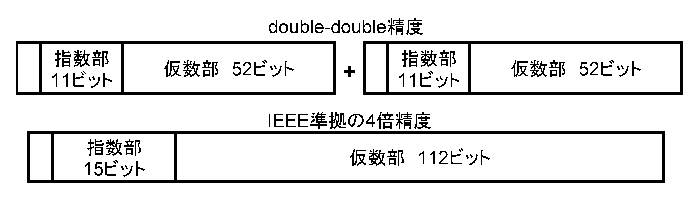
\includegraphics{double-double.eps}
\caption{double-double$B7?$N%S%C%H?t(B}
\label{fig:residual}
  }
\end{figure}

\subsection{4$BG\@:EY1i;;$N;HMQ(B}
\label{sec:testprog4}
Toepliz$B9TNs(B
\[
A = \left(
\begin{array}{cccccc}
2 & 1 &   &  &  & \\
0 & 2 & 1 &  &  & \\
\gamma & 0& 2 & 1 &  & \\
 & \ddots & \ddots & \ddots & \ddots & \\
 &  &   \gamma &0 &       2   & 1 \\
 &  &  &   \gamma & 0& 2 \\
\end{array}
\right)
\]
$B$KBP$9$k@~7?J}Dx<0(B$Ax=b$$B$r;XDj$5$l$?2rK!$G2r$-(B, $B2r$rI8=`=PNO$K=q$-=P$9(B
$B8!>Z%W%m%0%i%`$,(B\verb|test5.c|$B$G$"$k(B. 
$B1&JU%Y%/%H%k(B$b$$B$O2r(B$x$$B$,$9$Y$F(B$1$$B$H$J$k$h$&(B
$B@_Dj$5$l$k(B. $n$$B$O9TNs(B$A$$B$N<!?t$G$"$k(B. 
\verb|test5|$B$K$*$$$F(B, 
\newpage
{\bf $BG\@:EY$N>l9g(B}\\
\verb+      > ./test5 200 2.0 -f double+ \\
$B$^$?$O(B \\
\verb+      > ./test5 200 2.0+ \\
$B$HF~NO$7$F<B9T$9$k$H(B, $B0J2<$N7k2L$,F@$i$l$k(B. 

\begin{verbatim}
n = 200, gamma = 2.000000

initial vector x      : 0
precision             : double
linear solver         : BiCG
preconditioner        : none
convergence condition : ||b-Ax||_2 <= 1.0e-12 * ||b-Ax_0||_2
matrix storage format : CSR
linear solver status  : normal end

BiCG: number of iterations = 1001 (double = 1001, quad = 0)
BiCG: elapsed time         = 2.044368e-02 sec.
BiCG:   preconditioner     = 4.768372e-06 sec.
BiCG:     matrix creation  = 4.768372e-06 sec.
BiCG:   linear solver      = 2.043891e-02 sec.
BiCG: relative residual    = 8.917591e+01
\end{verbatim}

{\bf 4$BG\@:EY$N>l9g(B}\\
\verb+      > ./test5 200 2.0 -f quad+\\
$B$HF~NO$7$F<B9T$9$k$H(B, $B0J2<$N7k2L$,F@$i$l$k(B. 

\begin{verbatim}
n = 200, gamma = 2.000000

initial vector x      : 0
precision             : quad
linear solver         : BiCG
preconditioner        : none
convergence condition : ||b-Ax||_2 <= 1.0e-12 * ||b-Ax_0||_2
matrix storage format : CSR
linear solver status  : normal end

BiCG: number of iterations = 230 (double = 230, quad = 0)
BiCG: elapsed time         = 2.267408e-02 sec.
BiCG:   preconditioner     = 4.549026e-04 sec.
BiCG:     matrix creation  = 5.006790e-06 sec.
BiCG:   linear solver      = 2.221918e-02 sec.
BiCG: relative residual    = 6.499145e-11
\end{verbatim}

\newpage
\section{$B9TNs3JG<7A<0(B}
\label{sec:storages}
$BK\@a$G$O(B, $B%i%$%V%i%j$G;HMQ$G$-$k9TNs$N3JG<7A<0$K$D$$$F=R$Y$k(B. 
$B9TNs$N9T(B($BNs(B)$BHV9f$O(B0$B$+$i;O$^$k$b$N$H$9$k(B. 
$B<!?t(B$n \times n$$B$N9TNs(B$A=(a_{ij})$$B$NHsNmMWAG?t$r(B$nnz$$B$H$9$k(B. 

\subsection{Compressed Sparse Row (CSR)}
CSR$B7A<0$G$O(B, $B%G!<%?$r(B3$B$D$NG[Ns(B({\ttfamily ptr,index,value})$B$K3JG<$9$k(B. 
\begin{itemize}
\item $BD9$5(B$nnz$$B$NG\@:EYG[Ns(B{\ttfamily value}$B$O(B, $B9TNs(B$A$$B$NHsNmMWAG$NCM$r9TJ}8~$K1h$C$F3JG<$9$k(B. 
\item $BD9$5(B$nnz$$B$N@0?tG[Ns(B{\ttfamily index}$B$O(B, $BG[Ns(B{\ttfamily value}$B$K3JG<$5$l$?HsNmMWAG$NNsHV9f$r3JG<$9$k(B. 
\item $BD9$5(B$n+1$$B$N@0?tG[Ns(B{\ttfamily ptr}$B$O(B, $BG[Ns(B{\ttfamily value}$B$H(B{\ttfamily index}$B$N3F9T$N3+;O0LCV$r3JG<$9$k(B. 
\end{itemize}

\subsubsection{$B9TNs$N:n@.(B ($BC`<!!&%^%k%A%9%l%C%I4D6-(B)}
$B9TNs(B$A$$B$N(BCSR$B7A<0$G$N3JG<J}K!$r?^(B\ref{fig:storage01}$B$K<($9(B. 
$B$3$N9TNs$r(BCSR$B7A<0$G:n@.$9$k>l9g(B, $B%W%m%0%i%`$O0J2<$N$h$&$K5-=R$9$k(B. 
\begin{figure}[h]
{\centering 
\begin{minipage}{0.3\textwidth}
\begin{flushright}
$ \label{eq:mata}
A = \left(
\begin{array}{cccc}
11 &    &    &    \\
21 & 22 &    &    \\
   & 32 & 33 &    \\
41 &    & 43 & 44 \\
\end{array}\right)
$
\end{flushright}
\end{minipage}
\begin{minipage}{0.6\textwidth}
\begin{flushleft}
\includegraphics{storage01.eps} 
\end{flushleft}
\end{minipage}
\caption{CSR$B7A<0$N%G!<%?9=B$(B ($BC`<!!&%^%k%A%9%l%C%I4D6-(B)}\label{fig:storage01}}
\end{figure}
\begin{itembox}[l]{$BC`<!!&%^%k%A%9%l%C%I4D6-(B}
\small
\begin{verbatim}
 1: LIS_INT n,nnz;
 2: LIS_INT *ptr,*index;
 3: LIS_SCALAR *value;
 4: LIS_MATRIX A;
 5: n = 4; nnz = 8;
 6: ptr   = (LIS_INT *)malloc( (n+1)*sizeof(int) );
 7: index = (LIS_INT *)malloc( nnz*sizeof(int) );
 8: value = (LIS_SCALAR *)malloc( nnz*sizeof(LIS_SCALAR) );
 9: lis_matrix_create(0,&A);
10: lis_matrix_set_size(A,0,n);
11:
12: ptr[0] = 0; ptr[1] = 1; ptr[2] = 3; ptr[3] = 5; ptr[4] = 8;
13: index[0] =  0; index[1] =  0; index[2] =  1; index[3] =  1;
14: index[4] =  2; index[5] =  0; index[6] =  2; index[7] =  3;
15: value[0] = 11; value[1] = 21; value[2] = 22; value[3] = 32;
16: value[4] = 33; value[5] = 41; value[6] = 43; value[7] = 44;
17:
18: lis_matrix_set_csr(nnz,ptr,index,value,A);
19: lis_matrix_assemble(A);
\end{verbatim}
\end{itembox}

\subsubsection{$B9TNs$N:n@.(B ($B%^%k%A%W%m%;%94D6-(B)}
2$B%W%m%;%9>e$X$N9TNs(B$A$$B$N(BCSR$B7A<0$G$N3JG<J}K!$r?^(B\ref{fig:storage01_mpi}$B$K<($9(B. 
2$B%W%m%;%9>e$K$3$N9TNs$r(BCSR$B7A<0$G:n@.$9$k>l9g(B, $B%W%m%0%i%`$O0J2<$N$h$&$K5-=R$9$k(B. 
\begin{figure}[h]
{\centering 
\includegraphics{storage01_mpi.eps} 
\caption{CSR$B7A<0$N%G!<%?9=B$(B ($B%^%k%A%W%m%;%94D6-(B)}\label{fig:storage01_mpi}}
\end{figure}
\begin{itembox}[l]{$B%^%k%A%W%m%;%94D6-(B}
\small
\begin{verbatim}
 1: LIS_INT i,k,n,nnz,my_rank;
 2: LIS_INT *ptr,*index;
 3: LIS_SCALAR *value;
 4: LIS_MATRIX A;
 5: MPI_Comm_rank(MPI_COMM_WORLD,&my_rank);
 6: if( my_rank==0 ) {n = 2; nnz = 3;}
 7: else             {n = 2; nnz = 5;}
 8: ptr   = (LIS_INT *)malloc( (n+1)*sizeof(int) );
 9: index = (LIS_INT *)malloc( nnz*sizeof(int) );
10: value = (LIS_SCALAR *)malloc( nnz*sizeof(LIS_SCALAR) );
11: lis_matrix_create(MPI_COMM_WORLD,&A);
12: lis_matrix_set_size(A,n,0);
13: if( my_rank==0 ) {
14:     ptr[0] = 0; ptr[1] = 1; ptr[2] = 3;
15:     index[0] =  0; index[1] =  0; index[2] =  1;
16:     value[0] = 11; value[1] = 21; value[2] = 22;}
17: else {
18:     ptr[0] = 0; ptr[1] = 2; ptr[2] = 5;
19:     index[0] =  1; index[1] =  2; index[2] =  0; index[3] =  2; index[4] =  3;
20:     value[0] = 32; value[1] = 33; value[2] = 41; value[3] = 43; value[4] = 44;}
21: lis_matrix_set_csr(nnz,ptr,index,value,A);
22: lis_matrix_assemble(A);
\end{verbatim}
\end{itembox}

\subsubsection{$B4XO"$9$k4X?t(B}
\noindent
{\bf $BG[Ns$N4XO"IU$1(B}

CSR$B7A<0$NG[Ns$r9TNs(B$A$$B$K4XO"IU$1$k$K$O(B, $B4X?t(B

\begin{itemize}
\item \verb|C       LIS_INT lis_matrix_set_csr(LIS_INT nnz, LIS_INT ptr[], LIS_INT index[],|\\
      \verb| LIS_SCALAR value[], LIS_MATRIX A)|
\item \verb|Fortran subroutine lis_matrix_set_csr(LIS_INTEGER nnz, LIS_INTEGER ptr(),|\\
      \verb| LIS_INTEGER index(), LIS_SCALAR value(), LIS_MATRIX A, LIS_INTEGER ierr)|
\end{itemize}

$B$rMQ$$$k(B. 

\newpage
\subsection{Compressed Sparse Column (CSC)}
CSC$B7A<0$G$O(B, $B%G!<%?$r(B3$B$D$NG[Ns(B({\ttfamily ptr,index,value})$B$K3JG<$9$k(B. 
\begin{itemize}
\item $BD9$5(B$nnz$$B$NG\@:EYG[Ns(B{\ttfamily value}$B$O(B, $B9TNs(B$A$$B$NHsNmMWAG$NCM$rNsJ}8~$K1h$C$F3JG<$9$k(B. 
\item $BD9$5(B$nnz$$B$N@0?tG[Ns(B{\ttfamily index}$B$O(B, $BG[Ns(B{\ttfamily value}$B$K3JG<$5$l$?HsNmMWAG$N9THV9f$r3JG<$9$k(B. 
\item $BD9$5(B$n+1$$B$N@0?tG[Ns(B{\ttfamily ptr}$B$O(B, $BG[Ns(B{\ttfamily value}$B$H(B{\ttfamily index}$B$N3FNs$N3+;O0LCV$r3JG<$9$k(B. 
\end{itemize}

\subsubsection{$B9TNs$N:n@.(B ($BC`<!!&%^%k%A%9%l%C%I4D6-(B)}
$B9TNs(B$A$$B$N(BCSC$B7A<0$G$N3JG<J}K!$r?^(B\ref{fig:storage02}$B$K<($9(B. 
$B$3$N9TNs$r(BCSC$B7A<0$G:n@.$9$k>l9g(B, $B%W%m%0%i%`$O0J2<$N$h$&$K5-=R$9$k(B. 

\begin{figure}[h]
{\centering 
\begin{minipage}{0.3\textwidth}
\begin{flushright}
$ 
A = \left(
\begin{array}{cccc}
11 &    &    &    \\
21 & 22 &    &    \\
   & 32 & 33 &    \\
41 &    & 43 & 44 \\
\end{array}\right)
$
\end{flushright}
\end{minipage}
\begin{minipage}{0.6\textwidth}
\begin{flushleft}
\includegraphics{storage02.eps} 
\end{flushleft}
\end{minipage}
\caption{CSC$B7A<0$N%G!<%?9=B$(B ($BC`<!!&%^%k%A%9%l%C%I4D6-(B)}\label{fig:storage02}}
\end{figure}
\begin{itembox}[l]{$BC`<!!&%^%k%A%9%l%C%I4D6-(B}
\small
\begin{verbatim}
 1: LIS_INT n,nnz;
 2: LIS_INT *ptr,*index;
 3: LIS_SCALAR *value;
 4: LIS_MATRIX A;
 5: n = 4; nnz = 8;
 6: ptr   = (LIS_INT *)malloc( (n+1)*sizeof(int) );
 7: index = (LIS_INT *)malloc( nnz*sizeof(int) );
 8: value = (LIS_SCALAR *)malloc( nnz*sizeof(LIS_SCALAR) );
 9: lis_matrix_create(0,&A);
10: lis_matrix_set_size(A,0,n);
11:
12: ptr[0] = 0; ptr[1] = 3; ptr[2] = 5; ptr[3] = 7; ptr[4] = 8;
13: index[0] =  0; index[1] =  1; index[2] =  3; index[3] =  1;
14: index[4] =  2; index[5] =  2; index[6] =  3; index[7] =  3;
15: value[0] = 11; value[1] = 21; value[2] = 41; value[3] = 22;
16: value[4] = 32; value[5] = 33; value[6] = 43; value[7] = 44;
17:
18: lis_matrix_set_csc(nnz,ptr,index,value,A);
19: lis_matrix_assemble(A);
\end{verbatim}
\end{itembox}

\newpage
\subsubsection{$B9TNs$N:n@.(B ($B%^%k%A%W%m%;%94D6-(B)}
2$B%W%m%;%9>e$X$N9TNs(B$A$$B$N(BCSC$B7A<0$G$N3JG<J}K!$r?^(B\ref{fig:storage02_mpi}$B$K(B
$B<($9(B. 
2$B%W%m%;%9>e$K$3$N9TNs$r(BCSC$B7A<0$G:n@.$9$k>l9g(B, $B%W%m%0%i%`$O0J2<$N$h$&$K5-=R$9$k(B. 
\begin{figure}[h]
{\centering 
\includegraphics{storage02_mpi.eps} 
\caption{CSC$B7A<0$N%G!<%?9=B$(B ($B%^%k%A%W%m%;%94D6-(B)}\label{fig:storage02_mpi}}
\end{figure}
\begin{itembox}[l]{$B%^%k%A%W%m%;%94D6-(B}
\small
\begin{verbatim}
 1: LIS_INT i,k,n,nnz,my_rank;
 2: LIS_INT *ptr,*index;
 3: LIS_SCALAR *value;
 4: LIS_MATRIX A;
 5: MPI_Comm_rank(MPI_COMM_WORLD,&my_rank);
 6: if( my_rank==0 ) {n = 2; nnz = 3;}
 7: else             {n = 2; nnz = 5;}
 8: ptr   = (LIS_INT *)malloc( (n+1)*sizeof(int) );
 9: index = (LIS_INT *)malloc( nnz*sizeof(int) );
10: value = (LIS_SCALAR *)malloc( nnz*sizeof(LIS_SCALAR) );
11: lis_matrix_create(MPI_COMM_WORLD,&A);
12: lis_matrix_set_size(A,n,0);
13: if( my_rank==0 ) {
14:     ptr[0] = 0; ptr[1] = 3; ptr[2] = 5;
15:     index[0] =  0; index[1] =  1; index[2] =  3; index[3] =  1; index[4] =  2;
16:     value[0] = 11; value[1] = 21; value[2] = 41; value[3] = 22; value[4] = 32}
17: else {
18:     ptr[0] = 0; ptr[1] = 2; ptr[2] = 3;
19:     index[0] =  2; index[1] =  3; index[2] =  3;
20:     value[0] = 33; value[1] = 43; value[2] = 44;}
21: lis_matrix_set_csc(nnz,ptr,index,value,A);
22: lis_matrix_assemble(A);
\end{verbatim}
\end{itembox}

\subsubsection{$B4XO"$9$k4X?t(B}
\noindent
{\bf $BG[Ns$N4XO"IU$1(B}

CSC$B7A<0$NG[Ns$r9TNs(B$A$$B$K4XO"IU$1$k$K$O(B, $B4X?t(B
\begin{itemize}
\item \verb|C       LIS_INT lis_matrix_set_csc(LIS_INT nnz, LIS_INT ptr[], LIS_INT index[],|\\
      \verb| LIS_SCALAR value[], LIS_MATRIX A)|
\item \verb|Fortran subroutine lis_matrix_set_csc(LIS_INTEGER nnz, LIS_INTEGER ptr(),|\\
      \verb| LIS_INTEGER index(), LIS_SCALAR value(), LIS_MATRIX A, LIS_INTEGER ierr)|
\end{itemize}
$B$rMQ$$$k(B. 

\newpage
\subsection{Modified Compressed Sparse Row (MSR)}
MSR$B7A<0$G$O(B, $B%G!<%?$r(B2$B$D$NG[Ns(B({\ttfamily index,value})$B$K3JG<$9$k(B. $ndz$$B$rBP3QItJ,$NNmMWAG?t$H$9$k(B. 
\begin{itemize}
\item $BD9$5(B$nnz + ndz + 1$$B$NG\@:EYG[Ns(B{\ttfamily value}$B$O(B, 
$BBh(B$n$$BMWAG$^$G$O9TNs(B$A$$B$NBP3QItJ,$r3JG<$9$k(B. $BBh(B$n+1$$BMWAG$O;HMQ$7$J$$(B. $BBh(B
      $n+2$$BMWAG$+$i$O(B
$B9TNs(B$A$$B$NBP3QItJ,0J30$NHsNmMWAG$NCM$r9TJ}8~$K1h$C$F3JG<$9$k(B. 
\item $BD9$5(B$nnz + ndz + 1$$B$N@0?tG[Ns(B{\ttfamily index}$B$O(B, 
$BBh(B$n+1$$BMWAG$^$G$O9TNs(B$A$$B$NHsBP3QItJ,$N3F9T$N3+;O0LCV$r3JG<$9$k(B. 
$BBh(B$n+2$$BMWAG$+$i$O9TNs(B$A$$B$NHsBP3QItJ,$NG[Ns(B{\ttfamily value}$B$K3JG<$5$l$?HsNmMWAG$NNsHV9f$r3JG<$9$k(B. 
\end{itemize}

\subsubsection{$B9TNs$N:n@.(B ($BC`<!!&%^%k%A%9%l%C%I4D6-(B)}
$B9TNs(B$A$$B$N(BMSR$B7A<0$G$N3JG<J}K!$r?^(B\ref{fig:storage03}$B$K<($9(B. 
$B$3$N9TNs$r(BMSR$B7A<0$G:n@.$9$k>l9g(B, $B%W%m%0%i%`$O0J2<$N$h$&$K5-=R$9$k(B. 

\begin{figure}[h]
{\centering 
\begin{minipage}{0.3\textwidth}
\begin{flushright}
$ 
A = \left(
\begin{array}{cccc}
11 &    &    &    \\
21 & 22 &    &    \\
   & 32 & 33 &    \\
41 &    & 43 & 44 \\
\end{array}\right)
$
\end{flushright}
\end{minipage}
\begin{minipage}{0.6\textwidth}
\begin{flushleft}
\includegraphics{storage03.eps} 
\end{flushleft}
\end{minipage}
\caption{MSR$B7A<0$N%G!<%?9=B$(B ($BC`<!!&%^%k%A%9%l%C%I4D6-(B)}\label{fig:storage03}}
\end{figure}
\begin{itembox}[l]{$BC`<!!&%^%k%A%9%l%C%I4D6-(B}
\small
\begin{verbatim}
 1: LIS_INT n,nnz,ndz;
 2: LIS_INT *index;
 3: LIS_SCALAR *value;
 4: LIS_MATRIX A;
 5: n = 4; nnz = 8; ndz = 0;
 6: index = (LIS_INT *)malloc( (nnz+ndz+1)*sizeof(int) );
 7: value = (LIS_SCALAR *)malloc( (nnz+ndz+1)*sizeof(LIS_SCALAR) );
 8: lis_matrix_create(0,&A);
 9: lis_matrix_set_size(A,0,n);
10:
11: index[0] =  5; index[1] =  5; index[2] =  6; index[3] =  7;
12: index[4] =  9; index[5] =  0; index[6] =  1; index[7] =  0; index[8] =  2;
13: value[0] = 11; value[1] = 22; value[2] = 33; value[3] = 44;
14: value[4] =  0; value[5] = 21; value[6] = 32; value[7] = 41; value[8] = 43;
15:
16: lis_matrix_set_msr(nnz,ndz,index,value,A);
17: lis_matrix_assemble(A);
\end{verbatim}
\end{itembox}

\newpage
\subsubsection{$B9TNs$N:n@.(B ($B%^%k%A%W%m%;%94D6-(B)}
2$B%W%m%;%9>e$X$N9TNs(B$A$$B$N(BMSR$B7A<0$G$N3JG<J}K!$r?^(B\ref{fig:storage03_mpi}$B$K(B
$B<($9(B. 
2$B%W%m%;%9>e$K$3$N9TNs$r(BMSR$B7A<0$G:n@.$9$k>l9g(B, $B%W%m%0%i%`$O0J2<$N$h$&$K5-=R$9$k(B. 
\begin{figure}[h]
{\centering 
\includegraphics{storage03_mpi.eps} 
\caption{MSR$B7A<0$N%G!<%?9=B$(B ($B%^%k%A%W%m%;%94D6-(B)}\label{fig:storage03_mpi}}
\end{figure}
\begin{itembox}[l]{$B%^%k%A%W%m%;%94D6-(B}
\small
\begin{verbatim}
 1: LIS_INT i,k,n,nnz,ndz,my_rank;
 2: LIS_INT *index;
 3: LIS_SCALAR *value;
 4: LIS_MATRIX A;
 5: MPI_Comm_rank(MPI_COMM_WORLD,&my_rank);
 6: if( my_rank==0 ) {n = 2; nnz = 3; ndz = 0;}
 7: else             {n = 2; nnz = 5; ndz = 0;}
 8: index = (LIS_INT *)malloc( (nnz+ndz+1)*sizeof(int) );
 9: value = (LIS_SCALAR *)malloc( (nnz+ndz+1)*sizeof(LIS_SCALAR) );
10: lis_matrix_create(MPI_COMM_WORLD,&A);
11: lis_matrix_set_size(A,n,0);
12: if( my_rank==0 ) {
13:     index[0] =  3; index[1] =  3; index[2] =  4; index[3] =  0;
14:     value[0] = 11; value[1] = 22; value[2] =  0; value[3] = 21;}
15: else {
16:     index[0] =  3; index[1] =  4; index[2] =  6; index[3] =  1;
17:     index[4] =  0; index[5] =  2;
18:     value[0] = 33; value[1] = 44; value[2] =  0; value[3] = 32;
19:     value[4] = 41; value[5] = 43;}
20: lis_matrix_set_msr(nnz,ndz,index,value,A);
21: lis_matrix_assemble(A);
\end{verbatim}
\end{itembox}

\subsubsection{$B4XO"$9$k4X?t(B}
\noindent
{\bf $BG[Ns$N4XO"IU$1(B}

MSR$B7A<0$NG[Ns$r9TNs(B$A$$B$K4XO"IU$1$k$K$O(B, $B4X?t(B
\begin{itemize}
\item \verb|C       LIS_INT lis_matrix_set_msr(LIS_INT nnz, LIS_INT ndz, LIS_INT index[],|\\
      \verb| LIS_SCALAR value[], LIS_MATRIX A)|
\item \verb|Fortran subroutine lis_matrix_set_msr(LIS_INTEGER nnz, LIS_INTEGER ndz,|\\
      \verb| LIS_INTEGER index(), LIS_SCALAR value(), LIS_MATRIX A, LIS_INTEGER ierr)|
\end{itemize}
$B$rMQ$$$k(B. 

\newpage
\subsection{Diagonal (DIA)}
DIA$B7A<0$G$O(B, $B%G!<%?$r(B2$B$D$NG[Ns(B({\ttfamily index, value})$B$K3JG<$9$k(B. 
$nnd$$B$r9TNs(B$A$$B$NHsNm$JBP3QMWAG$NK\?t$H$9$k(B. 
\begin{itemize}
\item $BD9$5(B$nnd \times n$$B$NG\@:EYG[Ns(B{\ttfamily value}$B$O(B, $B9TNs(B$A$$B$NHsNm$JBP(B
      $B3QMWAG$NCM$r3JG<$9$k(B. 
\item $BD9$5(B$nnd$$B$N@0?tG[Ns(B{\ttfamily index}$B$O(B, $B<gBP3QMWAG$+$i3FBP3QMWAG$X$N%*%U%;%C%H$r3JG<$9$k(B. 
\end{itemize}
$B%^%k%A%9%l%C%I4D6-$G$O0J2<$N$h$&$K3JG<$9$k(B.\\
$B%G!<%?$r(B2$B$D$NG[Ns(B({\ttfamily index, value})$B$K3JG<$9$k(B. $nprocs$$B$r%9%l%C%I?t$H$9$k(B. 
$nnd_p$$B$r9TNs(B$A$$B$r9T%V%m%C%/J,3d$7$?ItJ,9TNs$NHsNm$JBP3QItJ,$NK\?t$H$9$k(B. 
$maxnnd$$B$r(B$nnd_p$$B$NCM$N:GBgCM$H$9$k(B. 
\begin{itemize}
\item $BD9$5(B$maxnnd \times n$$B$NG\@:EYG[Ns(B{\ttfamily value}$B$O(B, $B9TNs(B$A$$B$r9T%V(B
      $B%m%C%/J,3d$7$?ItJ,9TNs$NHsNm$JBP3QMWAG$NCM$r3JG<$9$k(B. 
\item $BD9$5(B$nprocs \times maxnnd$$B$N@0?tG[Ns(B{\ttfamily index}$B$O(B, $B<gBP3QMWAG$+$i3FBP3QMWAG$X$N%*%U%;%C%H$r3JG<$9$k(B. 
\end{itemize}

\subsubsection{$B9TNs$N:n@.(B ($BC`<!4D6-(B)}
$B9TNs(B$A$$B$N(BDIA$B7A<0$G$N3JG<J}K!$r?^(B\ref{fig:storage04}$B$K<($9(B. 
$B$3$N9TNs$r(BDIA$B7A<0$G:n@.$9$k>l9g(B, $B%W%m%0%i%`$O0J2<$N$h$&$K5-=R$9$k(B. 
\begin{figure}[h]
{\centering 
\begin{minipage}{0.3\textwidth}
\begin{flushright}
$ 
A = \left(
\begin{array}{cccc}
11 &    &    &    \\
21 & 22 &    &    \\
   & 32 & 33 &    \\
41 &    & 43 & 44 \\
\end{array}\right)
$
\end{flushright}
\end{minipage}
\begin{minipage}{0.6\textwidth}
\begin{flushleft}
\includegraphics{storage04.eps} 
\end{flushleft}
\end{minipage}
\caption{DIA$B7A<0$N%G!<%?9=B$(B ($BC`<!4D6-(B)}\label{fig:storage04}}
\end{figure}
\begin{itembox}[l]{$BC`<!4D6-(B}
\small
\begin{verbatim}
 1: LIS_INT n,nnd;
 2: LIS_INT *index;
 3: LIS_SCALAR *value;
 4: LIS_MATRIX A;
 5: n = 4; nnd = 3;
 6: index = (LIS_INT *)malloc( nnd*sizeof(int) );
 7: value = (LIS_SCALAR *)malloc( n*nnd*sizeof(LIS_SCALAR) );
 8: lis_matrix_create(0,&A);
 9: lis_matrix_set_size(A,0,n);
10:
11: index[0] = -3; index[1] = -1; index[2] =  0;
12: value[0] =  0; value[1] =  0; value[2] =  0; value[3] = 41;
13: value[4] =  0; value[5] = 21; value[6] = 32; value[7] = 43;
14: value[8] = 11; value[9] = 22; value[10]= 33; value[11]= 44;
15:
16: lis_matrix_set_dia(nnd,index,value,A);
17: lis_matrix_assemble(A);
\end{verbatim}
\end{itembox}

\subsubsection{$B9TNs$N:n@.(B ($B%^%k%A%9%l%C%I4D6-(B)}
2$B%9%l%C%I>e$X$N9TNs(B$A$$B$N(BDIA$B7A<0$G$N3JG<J}K!$r?^(B\ref{fig:storage04_omp}$B$K(B
$B<($9(B. 
2$B%9%l%C%I>e$K$3$N9TNs$r(BDIA$B7A<0$G:n@.$9$k>l9g(B, $B%W%m%0%i%`$O0J2<$N$h$&$K5-=R$9$k(B. 
\begin{figure}[h]
{\centering 
\includegraphics{storage04_omp.eps} 
\caption{DIA$B7A<0$N%G!<%?9=B$(B ($B%^%k%A%9%l%C%I4D6-(B)}\label{fig:storage04_omp}}
\end{figure}
\begin{itembox}[l]{$B%^%k%A%9%l%C%I4D6-(B}
\small
\begin{verbatim}
 1: LIS_INT n,maxnnd,nprocs;
 2: LIS_INT *index;
 3: LIS_SCALAR *value;
 4: LIS_MATRIX A;
 5: n = 4; maxnnd = 3; nprocs = 2;
 6: index = (LIS_INT *)malloc( maxnnd*sizeof(int) );
 7: value = (LIS_SCALAR *)malloc( n*maxnnd*sizeof(LIS_SCALAR) );
 8: lis_matrix_create(0,&A);
 9: lis_matrix_set_size(A,0,n);
10:
11: index[0] = -1; index[1] =  0; index[2] =  0; index[3] = -3; index[4] = -1; index[5] =  0;
12: value[0] =  0; value[1] = 21; value[2] = 11; value[3] = 22; value[4] =  0; value[5] =  0;
13: value[6] =  0; value[7] = 41; value[8] = 32; value[9] = 43; value[10]= 33; value[11]= 44;
14:
15: lis_matrix_set_dia(maxnnd,index,value,A);
16: lis_matrix_assemble(A);
\end{verbatim}
\end{itembox}
\newpage

\subsubsection{$B9TNs$N:n@.(B ($B%^%k%A%W%m%;%94D6-(B)}
2$B%W%m%;%9>e$X$N9TNs(B$A$$B$N(BDIA$B7A<0$G$N3JG<J}K!$r?^(B\ref{fig:storage04_mpi}$B$K(B
$B<($9(B. 
2$B%W%m%;%9>e$K$3$N9TNs$r(BDIA$B7A<0$G:n@.$9$k>l9g(B, $B%W%m%0%i%`$O0J2<$N$h$&$K5-=R$9$k(B. 
\begin{figure}[h]
{\centering 
\includegraphics{storage04_mpi.eps} 
\caption{DIA$B7A<0$N%G!<%?9=B$(B ($B%^%k%A%W%m%;%94D6-(B)}\label{fig:storage04_mpi}}
\end{figure}
\begin{itembox}[l]{$B%^%k%A%W%m%;%94D6-(B}
\small
\begin{verbatim}
 1: LIS_INT i,n,nnd,my_rank;
 2: LIS_INT *index;
 3: LIS_SCALAR *value;
 4: LIS_MATRIX A;
 5: MPI_Comm_rank(MPI_COMM_WORLD,&my_rank);
 6: if( my_rank==0 ) {n = 2; nnd = 2;}
 7: else             {n = 2; nnd = 3;}
 8: index = (LIS_INT *)malloc( nnd*sizeof(int) );
 9: value = (LIS_SCALAR *)malloc( n*nnd*sizeof(LIS_SCALAR) );
10: lis_matrix_create(MPI_COMM_WORLD,&A);
11: lis_matrix_set_size(A,n,0);
12: if( my_rank==0 ) {
13:     index[0] = -1; index[1] =  0;
14:     value[0] =  0; value[1] = 21; value[2] = 11; value[3] = 22;}
15: else {
16:     index[0] = -3; index[1] = -1; index[2] =  0;
17:     value[0] =  0; value[1] = 41; value[2] = 32; value[3] = 43; value[4] = 33;
18:     value[5] = 44;}
19: lis_matrix_set_dia(nnd,index,value,A);
20: lis_matrix_assemble(A);
\end{verbatim}
\end{itembox}

\subsubsection{$B4XO"$9$k4X?t(B}
\noindent
{\bf $BG[Ns$N4XO"IU$1(B}

DIA$B7A<0$NG[Ns$r9TNs(B$A$$B$K4XO"IU$1$k$K$O(B, $B4X?t(B
\begin{itemize}
\item \verb|C       LIS_INT lis_matrix_set_dia(LIS_INT nnd, LIS_INT index[],|\\
      \verb| LIS_SCALAR value[], LIS_MATRIX A)|
\item \verb|Fortran subroutine lis_matrix_set_dia(LIS_INTEGER nnd, LIS_INTEGER index(),|\\
      \verb| LIS_SCALAR value(), LIS_MATRIX A, LIS_INTEGER ierr)|
\end{itemize}
$B$rMQ$$$k(B. 

\newpage
\subsection{Ellpack-Itpack Generalized Diagonal (ELL)}
ELL$B7A<0$G$O(B, $B%G!<%?$r(B2$B$D$NG[Ns(B({\ttfamily index, value})$B$K3JG<$9$k(B. 
$maxnzr$$B$r9TNs(B$A$$B$N3F9T$G$NHsNmMWAG?t$N:GBgCM$H$9$k(B. 
\begin{itemize}
\item $BD9$5(B$maxnzr \times n$$B$NG\@:EYG[Ns(B{\ttfamily value}$B$O(B, $B9TNs(B$A$$B$N3F9T$NHsNmMWAG$NCM$rNsJ}8~$K1h$C$F3JG<$9$k(B. 
$B:G=i$NNs$O3F9T$N:G=i$NHsNmMWAG$+$i$J$k(B. $B$?$@$7(B, $B3JG<$9$kHsNmMWAG$,$J$$>l9g$O(B$0$$B$r3JG<$9$k(B. 
\item $BD9$5(B$maxnzr \times n$$B$N@0?tG[Ns(B{\ttfamily index}$B$O(B, 
$BG[Ns(B{\ttfamily value}$B$K3JG<$5$l$?HsNmMWAG$NNsHV9f$r3JG<$9$k(B. 
$B$?$@$7(B, $BBh(B$i$$B9T$NHsNmMWAG?t$r(B$nnz$$B$H$9$k$H(B{\tt index[$nnz \times n + i$]}$B$K$O$=$N9THV9f(B$i$$B$r3JG<$9$k(B. 
\end{itemize}

\subsubsection{$B9TNs$N:n@.(B ($BC`<!!&%^%k%A%9%l%C%I4D6-(B)}
$B9TNs(B$A$$B$N(BELL$B7A<0$G$N3JG<J}K!$r?^(B\ref{fig:storage05}$B$K<($9(B. 
$B$3$N9TNs$r(BELL$B7A<0$G:n@.$9$k>l9g(B, $B%W%m%0%i%`$O0J2<$N$h$&$K5-=R$9$k(B. 
\begin{figure}[h]
{\centering 
\begin{minipage}{0.3\textwidth}
\begin{flushright}
$ 
A = \left(
\begin{array}{cccc}
11 &    &    &    \\
21 & 22 &    &    \\
   & 32 & 33 &    \\
41 &    & 43 & 44 \\
\end{array}\right)
$
\end{flushright}
\end{minipage}
\begin{minipage}{0.6\textwidth}
\begin{flushleft}
\includegraphics{storage05.eps} 
\end{flushleft}
\end{minipage}
\caption{ELL$B7A<0$N%G!<%?9=B$(B ($BC`<!!&%^%k%A%9%l%C%I4D6-(B)}\label{fig:storage05}}
\end{figure}
\begin{itembox}[l]{$BC`<!!&%^%k%A%9%l%C%I4D6-(B}
\small
\begin{verbatim}
 1: LIS_INT n,maxnzr;
 2: LIS_INT *index;
 3: LIS_SCALAR *value;
 4: LIS_MATRIX A;
 5: n = 4; maxnzr = 3;
 6: index = (LIS_INT *)malloc( n*maxnzr*sizeof(int) );
 7: value = (LIS_SCALAR *)malloc( n*maxnzr*sizeof(LIS_SCALAR) );
 8: lis_matrix_create(0,&A);
 9: lis_matrix_set_size(A,0,n);
10:
11: index[0] =  0; index[1] =  0; index[2] =  1; index[3] =  0; index[4] =  0; index[5] =  1;
12: index[6] =  2; index[7] =  2; index[8] =  0; index[9] =  1; index[10]=  2; index[11]=  3;
13: value[0] = 11; value[1] = 21; value[2] = 32; value[3] = 41; value[4] =  0; value[5] = 22;
14: value[6] = 33; value[7] = 43; value[8] =  0; value[9] =  0; value[10]=  0; value[11]= 44;
15:
16: lis_matrix_set_ell(maxnzr,index,value,A);
17: lis_matrix_assemble(A);
\end{verbatim}
\end{itembox}

\newpage
\subsubsection{$B9TNs$N:n@.(B ($B%^%k%A%W%m%;%94D6-(B)}
2$B%W%m%;%9>e$X$N9TNs(B$A$$B$N(BELL$B7A<0$G$N3JG<J}K!$r?^(B\ref{fig:storage05_mpi}$B$K(B
$B<($9(B. 
2$B%W%m%;%9>e$K$3$N9TNs$r(BELL$B7A<0$G:n@.$9$k>l9g(B, $B%W%m%0%i%`$O0J2<$N$h$&$K5-=R$9$k(B. 
\begin{figure}[h]
{\centering 
\includegraphics{storage05_mpi.eps} 
\caption{ELL$B7A<0$N%G!<%?9=B$(B ($B%^%k%A%W%m%;%94D6-(B)}\label{fig:storage05_mpi}}
\end{figure}
\begin{itembox}[l]{$B%^%k%A%W%m%;%94D6-(B}
\small
\begin{verbatim}
 1: LIS_INT i,n,maxnzr,my_rank;
 2: LIS_INT *index;
 3: LIS_SCALAR *value;
 4: LIS_MATRIX A;
 5: MPI_Comm_rank(MPI_COMM_WORLD,&my_rank);
 6: if( my_rank==0 ) {n = 2; maxnzr = 2;}
 7: else             {n = 2; maxnzr = 3;}
 8: index = (LIS_INT *)malloc( n*maxnzr*sizeof(int) );
 9: value = (LIS_SCALAR *)malloc( n*maxnzr*sizeof(LIS_SCALAR) );
10: lis_matrix_create(MPI_COMM_WORLD,&A);
11: lis_matrix_set_size(A,n,0);
12: if( my_rank==0 ) {
13:     index[0] =  0; index[1] =  0; index[2] =  0; index[3] =  1;
14:     value[0] = 11; value[1] = 21; value[2] =  0; value[3] = 22;}
15: else {
16:     index[0] =  1; index[1] =  0; index[2] =  2; index[3] =  2; index[4] =  2;
17:     index[5] =  3;
18:     value[0] = 32; value[1] = 41; value[2] = 33; value[3] = 43; value[4] =  0;
19:     value[5] = 44;}
20: lis_matrix_set_ell(maxnzr,index,value,A);
21: lis_matrix_assemble(A);
\end{verbatim}
\end{itembox}

\subsubsection{$B4XO"$9$k4X?t(B}
\noindent
{\bf $BG[Ns$N4XO"IU$1(B}

ELL$B7A<0$NG[Ns$r9TNs(B$A$$B$K4XO"IU$1$k$K$O(B, $B4X?t(B
\begin{itemize}
\item \verb|C       LIS_INT lis_matrix_set_ell(LIS_INT maxnzr, LIS_INT index[],|\\
      \verb| LIS_SCALAR value[], LIS_MATRIX A)|
\item \verb|Fortran subroutine lis_matrix_set_ell(LIS_INTEGER maxnzr, LIS_INTEGER index(),|\\
      \verb| LIS_SCALAR value(), LIS_MATRIX A, LIS_INTEGER ierr)|
\end{itemize}
$B$rMQ$$$k(B. 

\newpage
\subsection{Jagged Diagonal (JAD)}
JAD$B7A<0$G$O(B, $B:G=i$K3F9T$NHsNmMWAG?t$NBg$-$$=g$K9T$NJB$SBX$($r9T$$(B, 
$B3F9T$NHsNmMWAG$rNsJ}8~$K1h$C$F3JG<$9$k(B. 
JAD$B7A<0$G$O(B, $B%G!<%?$r(B4$B$D$NG[Ns(B({\ttfamily perm, ptr, index, value})$B$K3JG<$9$k(B. 
$maxnzr$$B$r9TNs(B$A$$B$N3F9T$G$NHsNmMWAG?t$N:GBgCM$H$9$k(B. 
\begin{itemize}
\item $BD9$5(B$n$$B$N@0?tG[Ns(B{\ttfamily perm}$B$O(B, $BJB$SBX$($?9THV9f$r3JG<$9$k(B. 
\item $BD9$5(B$nnz$$B$NG\@:EYG[Ns(B{\ttfamily value}$B$O(B, $BJB$SBX$($i$l$?9TNs(B$A$$B$N5x(B
      $B;u>uBP3QMWAG$NCM$r3JG<$9$k(B. 
$B:G=i$N5x;u>uBP3QMWAG$O3F9T$NBh(B1$BHsNmMWAG$+$i$J$k(B. 
$B<!$N5x;u>uBP3QMWAG$O3F9T$NBh(B2$BHsNmMWAG$+$i$J$k(B. $B$3$l$r=g<!7+$jJV$7$F$$$/(B. 
\item $BD9$5(B$nnz$$B$N@0?tG[Ns(B{\ttfamily index}$B$O(B, $BG[Ns(B{\ttfamily value}$B$K3JG<$5$l$?HsNmMWAG$NNsHV9f$r3JG<$9$k(B. 
\item $BD9$5(B$maxnzr + 1$$B$N@0?tG[Ns(B{\ttfamily ptr}$B$O(B, $B3F5x;u>uBP3QMWAG$N3+;O0LCV$r3JG<$9$k(B. 
\end{itemize}
$B%^%k%A%9%l%C%I4D6-$G$O0J2<$N$h$&$K3JG<$9$k(B.\\
$B%G!<%?$r(B4$B$D$NG[Ns(B({\ttfamily perm, ptr, index, value})$B$K3JG<$9$k(B. 
$nprocs$$B$r%9%l%C%I?t$H$9$k(B. 
$maxnzr_p$$B$r9TNs(B$A$$B$r9T%V%m%C%/J,3d$7$?ItJ,9TNs$N3F9T$G$NHsNmMWAG?t$N:GBgCM$H$9$k(B. 
$maxmaxnzr$$B$OG[Ns(B$maxnzr_p$$B$NCM$N:GBgCM$G$"$k(B. 
\begin{itemize}
\item $BD9$5(B$n$$B$N@0?tG[Ns(B{\ttfamily perm}$B$O(B, $B9TNs(B$A$$B$r9T%V%m%C%/J,3d$7$?ItJ,9TNs$rJB$SBX$($?9THV9f$r3JG<$9$k(B. 
\item $BD9$5(B$nnz$$B$NG\@:EYG[Ns(B{\ttfamily value}$B$O(B, $BJB$SBX$($i$l$?9TNs(B$A$$B$N5x(B
      $B;u>uBP3QMWAG$NCM$r3JG<$9$k(B. 
$B:G=i$N5x;u>uBP3QMWAG$O3F9T$NBh(B1$BHsNmMWAG$+$i$J$k(B. 
$B<!$N5x;u>uBP3QMWAG$O3F9T$NBh(B2$BHsNmMWAG$+$i$J$k(B. $B$3$l$r=g<!7+$jJV$7$F$$$/(B. 
\item $BD9$5(B$nnz$$B$N@0?tG[Ns(B{\ttfamily index}$B$O(B, $BG[Ns(B{\ttfamily value}$B$K3JG<$5$l$?HsNmMWAG$NNsHV9f$r3JG<$9$k(B. 
\item $BD9$5(B$nprocs \times (maxmaxnzr + 1)$$B$N@0?tG[Ns(B{\ttfamily ptr}$B$O(B, $B9TNs(B
      $A$$B$r9T%V%m%C%/J,3d$7$?ItJ,9TNs$N3F5x;u>uBP3QMWAG$N3+;O0LCV$r3JG<$9$k(B. 
\end{itemize}

\newpage
\subsubsection{$B9TNs$N:n@.(B ($BC`<!4D6-(B)}
$B9TNs(B$A$$B$N(BJAD$B7A<0$G$N3JG<J}K!$r?^(B\ref{fig:storage06}$B$K<($9(B. 
$B$3$N9TNs$r(BJAD$B7A<0$G:n@.$9$k>l9g(B, $B%W%m%0%i%`$O0J2<$N$h$&$K5-=R$9$k(B. 
\begin{figure}[h]
{\centering 
\begin{minipage}{0.3\textwidth}
\begin{flushright}
$ 
A = \left(
\begin{array}{cccc}
11 &    &    &    \\
21 & 22 &    &    \\
   & 32 & 33 &    \\
41 &    & 43 & 44 \\
\end{array}\right)
$
\end{flushright}
\end{minipage}
\begin{minipage}{0.6\textwidth}
\begin{flushleft}
\includegraphics{storage06.eps} 
\end{flushleft}
\end{minipage}
\caption{JAD$B7A<0$N%G!<%?9=B$(B ($BC`<!4D6-(B)}\label{fig:storage06}}
\end{figure}
\begin{itembox}[l]{$BC`<!4D6-(B}
\small
\begin{verbatim}
 1: LIS_INT n,nnz,maxnzr;
 2: LIS_INT *perm,*ptr,*index;
 3: LIS_SCALAR *value;
 4: LIS_MATRIX A;
 5: n = 4; nnz = 8; maxnzr = 3;
 6: perm  = (LIS_INT *)malloc( n*sizeof(int) );
 7: ptr   = (LIS_INT *)malloc( (maxnzr+1)*sizeof(int) );
 8: index = (LIS_INT *)malloc( nnz*sizeof(int) );
 9: value = (LIS_SCALAR *)malloc( nnz*sizeof(LIS_SCALAR) );
10: lis_matrix_create(0,&A);
11: lis_matrix_set_size(A,0,n);
12:
13: perm[0] = 3; perm[1] = 1; perm[2] = 2; perm[3] = 0;
14: ptr[0]  = 0; ptr[1]  = 4; ptr[2]  = 7; ptr[3]  = 8;
15: index[0] =  0; index[1] =  0; index[2] =  1; index[3] =  0;
16: index[4] =  2; index[5] =  1; index[6] =  2; index[7] =  3;
17: value[0] = 41; value[1] = 21; value[2] = 32; value[3] = 11;
18: value[4] = 43; value[5] = 22; value[6] = 33; value[7] = 44;
19:
20: lis_matrix_set_jad(nnz,maxnzr,perm,ptr,index,value,A);
21: lis_matrix_assemble(A);
\end{verbatim}
\end{itembox}

\newpage
\subsubsection{$B9TNs$N:n@.(B ($B%^%k%A%9%l%C%I4D6-(B)}
2$B%9%l%C%I>e$X$N9TNs(B$A$$B$N(BJAD$B7A<0$G$N3JG<J}K!$r?^(B\ref{fig:storage06_omp}$B$K(B
$B<($9(B. 
2$B%9%l%C%I>e$K$3$N9TNs$r(BJAD$B7A<0$G:n@.$9$k>l9g(B, $B%W%m%0%i%`$O0J2<$N$h$&$K5-=R$9$k(B. 
\begin{figure}[h]
{\centering 
\includegraphics{storage06_omp.eps} 
\caption{JAD$B7A<0$N%G!<%?9=B$(B ($B%^%k%A%9%l%C%I4D6-(B)}\label{fig:storage06_omp}}
\end{figure}
\begin{itembox}[l]{$B%^%k%A%9%l%C%I4D6-(B}
\small
\begin{verbatim}
 1: LIS_INT n,nnz,maxmaxnzr,nprocs;
 2: LIS_INT *perm,*ptr,*index;
 3: LIS_SCALAR *value;
 4: LIS_MATRIX A;
 5: n = 4; nnz = 8; maxmaxnzr = 3; nprocs = 2;
 6: perm  = (LIS_INT *)malloc( n*sizeof(int) );
 7: ptr   = (LIS_INT *)malloc( nprocs*(maxmaxnzr+1)*sizeof(int) );
 8: index = (LIS_INT *)malloc( nnz*sizeof(int) );
 9: value = (LIS_SCALAR *)malloc( nnz*sizeof(LIS_SCALAR) );
10: lis_matrix_create(0,&A);
11: lis_matrix_set_size(A,0,n);
12:
13: perm[0] = 1; perm[1] = 0; perm[2] = 3; perm[3] = 2;
14: ptr[0]  = 0; ptr[1]  = 2; ptr[2]  = 3; ptr[3]  = 0;
15: ptr[4]  = 3; ptr[5]  = 5; ptr[6]  = 7; ptr[7]  = 8;
16: index[0] =  0; index[1] =  0; index[2] =  1; index[3] =  0;
17: index[4] =  1; index[5] =  2; index[6] =  2; index[7] =  3;
18: value[0] = 21; value[1] = 11; value[2] = 22; value[3] = 41;
19: value[4] = 32; value[5] = 43; value[6] = 33; value[7] = 44;
20:
21: lis_matrix_set_jad(nnz,maxmaxnzr,perm,ptr,index,value,A);
22: lis_matrix_assemble(A);
\end{verbatim}
\end{itembox}

\newpage
\subsubsection{$B9TNs$N:n@.(B ($B%^%k%A%W%m%;%94D6-(B)}
2$B%W%m%;%9>e$X$N9TNs(B$A$$B$N(BJAD$B7A<0$G$N3JG<J}K!$r?^(B\ref{fig:storage06_mpi}$B$K(B
$B<($9(B. 
2$B%W%m%;%9>e$K$3$N9TNs$r(BJAD$B7A<0$G:n@.$9$k>l9g(B, $B%W%m%0%i%`$O0J2<$N$h$&$K5-=R$9$k(B. 
\begin{figure}[h]
{\centering 
\includegraphics{storage06_mpi.eps} 
\caption{JAD$B7A<0$N%G!<%?9=B$(B ($B%^%k%A%W%m%;%94D6-(B)}\label{fig:storage06_mpi}}
\end{figure}
\begin{itembox}[l]{$B%^%k%A%W%m%;%94D6-(B}
\small
\begin{verbatim}
 1: LIS_INT i,n,nnz,maxnzr,my_rank;
 2: LIS_INT *perm,*ptr,*index;
 3: LIS_SCALAR *value;
 4: LIS_MATRIX A;
 5: MPI_Comm_rank(MPI_COMM_WORLD,&my_rank);
 6: if( my_rank==0 ) {n = 2; nnz = 3; maxnzr = 2;}
 7: else             {n = 2; nnz = 5; maxnzr = 3;}
 8: perm  = (LIS_INT *)malloc( n*sizeof(int) );
 9: ptr   = (LIS_INT *)malloc( (maxnzr+1)*sizeof(int) );
10: index = (LIS_INT *)malloc( nnz*sizeof(int) );
11: value = (LIS_SCALAR *)malloc( nnz*sizeof(LIS_SCALAR) );
12: lis_matrix_create(MPI_COMM_WORLD,&A);
13: lis_matrix_set_size(A,n,0);
14: if( my_rank==0 ) {
15:     perm[0] = 1; perm[1] = 0;
16:     ptr[0]  = 0; ptr[1]  = 2; ptr[2]  = 3;
17:     index[0] =  0; index[1] =  0; index[2] =  1;
18:     value[0] = 21; value[1] = 11; value[2] = 22;}
19: else {
20:     perm[0] = 3; perm[1] = 2;
21:     ptr[0]  = 0; ptr[1]  = 2; ptr[2]  = 4; ptr[3]  = 5;
22:     index[0] =  0; index[1] =  1; index[2] =  2; index[3] =  2; index[4] =  3;
23:     value[0] = 41; value[1] = 32; value[2] = 43; value[3] = 33; value[4] = 44;}
24: lis_matrix_set_jad(nnz,maxnzr,perm,ptr,index,value,A);
25: lis_matrix_assemble(A);
\end{verbatim}
\end{itembox}

\subsubsection{$B4XO"$9$k4X?t(B}
\noindent
{\bf $BG[Ns$N4XO"IU$1(B}

JAD$B7A<0$NG[Ns$r9TNs(B$A$$B$K4XO"IU$1$k$K$O(B, $B4X?t(B
\begin{itemize}
\item \verb|C       LIS_INT lis_matrix_set_jad(LIS_INT nnz, LIS_INT maxnzr, LIS_INT perm[],|\\
      \verb| LIS_INT ptr[], LIS_INT index[], LIS_SCALAR value[], LIS_MATRIX A)|
\item \verb|Fortran subroutine lis_matrix_set_jad(LIS_INTEGER nnz, LIS_INTEGER maxnzr,|\\
      \verb| LIS_INTEGER perm(), LIS_INTEGER ptr(), LIS_INTEGER index(), LIS_SCALAR value(),|\\
      \verb| LIS_MATRIX A, LIS_INTEGER ierr)|
\end{itemize}
$B$rMQ$$$k(B. 

\newpage
\subsection{Block Sparse Row (BSR)}
BSR$B7A<0$G$O(B, $B9TNs$r(B$r \times c$$B$NBg$-$5$NItJ,9TNs(B ($B%V%m%C%/$H8F$V(B) $B$KJ,2r$9$k(B. 
BSR$B7A<0$G$O(B, CSR$B7A<0$HF1MM$N<j=g$GHsNm%V%m%C%/(B ($B>/$J$/$H$b(B1$B$D$N(B
$BHsNmMWAG$,B8:_$9$k(B) $B$r3JG<$9$k(B. 
$nr=n/r$, $bnnz$$B$r(B$A$$B$NHsNm%V%m%C%/?t$H$9$k(B. 
BSR$B7A<0$G$O(B, $B%G!<%?$r(B3$B$D$NG[Ns(B({\ttfamily bptr, bindex, value})$B$K3JG<$9$k(B. 
\begin{itemize}
\item $BD9$5(B$bnnz \times r \times c$$B$NG\@:EYG[Ns(B{\ttfamily value}$B$O(B, $BHsNm%V%m%C%/$NA4MWAG$NCM$r3JG<$9$k(B. 
\item $BD9$5(B$bnnz$$B$N@0?tG[Ns(B{\ttfamily bindex}$B$O(B, $BHsNm%V%m%C%/$N%V%m%C%/NsHV9f$r3JG<$9$k(B. 
\item $BD9$5(B$nr+1$$B$N@0?tG[Ns(B{\ttfamily bptr}$B$O(B, $BG[Ns(B{\ttfamily bindex}$B$N%V%m%C%/9T$N3+;O0LCV$r3JG<$9$k(B. 
\end{itemize}

\subsubsection{$B9TNs$N:n@.(B ($BC`<!!&%^%k%A%9%l%C%I4D6-(B)}
$B9TNs(B$A$$B$N(BBSR$B7A<0$G$N3JG<J}K!$r?^(B\ref{fig:storage07}$B$K<($9(B. 
$B$3$N9TNs$r(BBSR$B7A<0$G:n@.$9$k>l9g(B, $B%W%m%0%i%`$O0J2<$N$h$&$K5-=R$9$k(B. 
\begin{figure}[h]
{\centering 
\begin{minipage}{0.3\textwidth}
\begin{flushright}
$ 
A = \left(
\begin{array}{cc|cc}
11 &    &    &    \\
21 & 22 &    &    \\ \hline
   & 32 & 33 &    \\
41 &    & 43 & 44 \\
\end{array}\right)
$
\end{flushright}
\end{minipage}
\begin{minipage}{0.6\textwidth}
\begin{flushleft}
\includegraphics{storage07.eps} 
\end{flushleft}
\end{minipage}
\caption{BSR$B7A<0$N%G!<%?9=B$(B ($BC`<!!&%^%k%A%9%l%C%I4D6-(B)}\label{fig:storage07}}
\end{figure}
\begin{itembox}[l]{$BC`<!!&%^%k%A%9%l%C%I4D6-(B}
\small
\begin{verbatim}
 1: LIS_INT n,bnr,bnc,nr,nc,bnnz;
 2: LIS_INT *bptr,*bindex;
 3: LIS_SCALAR *value;
 4: LIS_MATRIX A;
 5: n = 4; bnr = 2; bnc = 2; bnnz = 3; nr = (n-1)/bnr+1; nc = (n-1)/bnc+1;
 6: bptr   = (LIS_INT *)malloc( (nr+1)*sizeof(int) );
 7: bindex = (LIS_INT *)malloc( bnnz*sizeof(int) );
 8: value  = (LIS_SCALAR *)malloc( bnr*bnc*bnnz*sizeof(LIS_SCALAR) );
 9: lis_matrix_create(0,&A);
10: lis_matrix_set_size(A,0,n);
11:
12: bptr[0] = 0; bptr[1] = 1; bptr[2] = 3;
13: bindex[0] =  0; bindex[1] =  0; bindex[2] =  1;
14: value[0]  = 11; value[1] = 21; value[2] =  0; value[3] = 22;
15: value[4]  =  0; value[5] = 41; value[6] = 32; value[7] =  0;
16: value[8]  = 33; value[9] = 43; value[10]=  0; value[11]= 44;
17:
18: lis_matrix_set_bsr(bnr,bnc,bnnz,bptr,bindex,value,A);
19: lis_matrix_assemble(A);
\end{verbatim}
\end{itembox}

\newpage
\subsubsection{$B9TNs$N:n@.(B ($B%^%k%A%W%m%;%94D6-(B)}
2$B%W%m%;%9>e$X$N9TNs(B$A$$B$N(BBSR$B7A<0$G$N3JG<J}K!$r?^(B\ref{fig:storage07_mpi}$B$K(B
$B<($9(B. 
2$B%W%m%;%9>e$K$3$N9TNs$r(BBSR$B7A<0$G:n@.$9$k>l9g(B, $B%W%m%0%i%`$O0J2<$N$h$&$K5-=R$9$k(B. 
\begin{figure}[h]
{\centering 
\includegraphics{storage07_mpi.eps} 
\caption{BSR$B7A<0$N%G!<%?9=B$(B ($B%^%k%A%W%m%;%94D6-(B)}\label{fig:storage07_mpi}}
\end{figure}
\begin{itembox}[l]{$B%^%k%A%W%m%;%94D6-(B}
\small
\begin{verbatim}
 1: LIS_INT n,bnr,bnc,nr,nc,bnnz,my_rank;
 2: LIS_INT *bptr,*bindex;
 3: LIS_SCALAR *value;
 4: LIS_MATRIX A;
 5: MPI_Comm_rank(MPI_COMM_WORLD,&my_rank);
 6: if( my_rank==0 ) {n = 2; bnr = 2; bnc = 2; bnnz = 1; nr = (n-1)/bnr+1; nc = (n-1)/bnc+1;}
 7: else             {n = 2; bnr = 2; bnc = 2; bnnz = 2; nr = (n-1)/bnr+1; nc = (n-1)/bnc+1;}
 8: bptr   = (LIS_INT *)malloc( (nr+1)*sizeof(int) );
 9: bindex = (LIS_INT *)malloc( bnnz*sizeof(int) );
10: value  = (LIS_SCALAR *)malloc( bnr*bnc*bnnz*sizeof(LIS_SCALAR) );
11: lis_matrix_create(MPI_COMM_WORLD,&A);
12: lis_matrix_set_size(A,n,0);
13: if( my_rank==0 ) {
14:     bptr[0] = 0; bptr[1] = 1;
15:     bindex[0] =  0;
16:     value[0]  = 11; value[1] = 21; value[2] =  0; value[3] = 22;}
17: else {
18:     bptr[0] = 0; bptr[1] = 2;
19:     bindex[0] =  0; bindex[1] =  1;
20:     value[0]  =  0; value[1]  = 41; value[2] = 32; value[3] =  0;
21:     value[4]  = 33; value[5]  = 43; value[6] =  0; value[7] = 44;}
22: lis_matrix_set_bsr(bnr,bnc,bnnz,bptr,bindex,value,A);
23: lis_matrix_assemble(A);
\end{verbatim}
\end{itembox}

\subsubsection{$B4XO"$9$k4X?t(B}
\noindent
{\bf $BG[Ns$N4XO"IU$1(B}

BSR$B7A<0$NG[Ns$r9TNs(B$A$$B$K4XO"IU$1$k$K$O(B, $B4X?t(B
\begin{itemize}
\item \verb|C       LIS_INT lis_matrix_set_bsr(LIS_INT bnr, LIS_INT bnc, LIS_INT bnnz,|\\
      \verb| LIS_INT bptr[], LIS_INT bindex[], LIS_SCALAR value[], LIS_MATRIX A)|
\item \verb|Fortran subroutine lis_matrix_set_bsr(LIS_INTEGER bnr, LIS_INTEGER bnc,|\\
      \verb| LIS_INTEGER bnnz, LIS_INTEGER bptr(), LIS_INTEGER bindex(), LIS_SCALAR value(),|\\
      \verb| LIS_MATRIX A, LIS_INTEGER ierr)|
\end{itemize}
$B$rMQ$$$k(B. 

\subsection{Block Sparse Column (BSC)}
BSC$B7A<0$G$O(B, $B9TNs$r(B$r \times c$$B$NBg$-$5$NItJ,9TNs(B ($B%V%m%C%/$H8F$V(B) $B$KJ,2r$9$k(B. 
BSC$B7A<0$G$O(B, CSC$B7A<0$HF1MM$N<j=g$GHsNm%V%m%C%/(B ($B>/$J$/$H$b(B1$B$D$N(B
$BHsNmMWAG$,B8:_$9$k(B) $B$r3JG<$9$k(B. 
$nc=n/c$, $bnnz$$B$r(B$A$$B$NHsNm%V%m%C%/?t$H$9$k(B. 
BSC$B7A<0$G$O(B, $B%G!<%?$r(B3$B$D$NG[Ns(B({\ttfamily bptr, bindex, value})$B$K3JG<$9$k(B. 
\begin{itemize}
\item $BD9$5(B$bnnz \times r \times c$$B$NG\@:EYG[Ns(B{\ttfamily value}$B$O(B, $BHsNm%V%m%C%/$NA4MWAG$NCM$r3JG<$9$k(B. 
\item $BD9$5(B$bnnz$$B$N@0?tG[Ns(B{\ttfamily bindex}$B$O(B, $BHsNm%V%m%C%/$N%V%m%C%/9THV9f$r3JG<$9$k(B. 
\item $BD9$5(B$nc+1$$B$N@0?tG[Ns(B{\ttfamily bptr}$B$O(B, $BG[Ns(B{\ttfamily bindex}$B$N%V%m%C%/Ns$N3+;O0LCV$r3JG<$9$k(B. 
\end{itemize}

\subsubsection{$B9TNs$N:n@.(B ($BC`<!!&%^%k%A%9%l%C%I4D6-(B)}
$B9TNs(B$A$$B$N(BBSC$B7A<0$G$N3JG<J}K!$r?^(B\ref{fig:storage08}$B$K<($9(B. 
$B$3$N9TNs$r(BBSC$B7A<0$G:n@.$9$k>l9g(B, $B%W%m%0%i%`$O0J2<$N$h$&$K5-=R$9$k(B. 
\begin{figure}[h]
{\centering 
\begin{minipage}{0.3\textwidth}
\begin{flushright}
$ 
A = \left(
\begin{array}{cc|cc}
11 &    &    &    \\
21 & 22 &    &    \\ \hline
   & 32 & 33 &    \\
41 &    & 43 & 44 \\
\end{array}\right)
$
\end{flushright}
\end{minipage}
\begin{minipage}{0.6\textwidth}
\begin{flushleft}
\includegraphics{storage08.eps} 
\end{flushleft}
\end{minipage}
\caption{BSC$B7A<0$N%G!<%?9=B$(B ($BC`<!!&%^%k%A%9%l%C%I4D6-(B)}\label{fig:storage08}}
\end{figure}
\begin{itembox}[l]{$BC`<!!&%^%k%A%9%l%C%I4D6-(B}
\small
\begin{verbatim}
 1: LIS_INT n,bnr,bnc,nr,nc,bnnz;
 2: LIS_INT *bptr,*bindex;
 3: LIS_SCALAR *value;
 4: LIS_MATRIX A;
 5: n = 4; bnr = 2; bnc = 2; bnnz = 3; nr = (n-1)/bnr+1; nc = (n-1)/bnc+1;
 6: bptr   = (LIS_INT *)malloc( (nc+1)*sizeof(int) );
 7: bindex = (LIS_INT *)malloc( bnnz*sizeof(int) );
 8: value  = (LIS_SCALAR *)malloc( bnr*bnc*bnnz*sizeof(LIS_SCALAR) );
 9: lis_matrix_create(0,&A);
10: lis_matrix_set_size(A,0,n);
11:
12: bptr[0] = 0; bptr[1] = 1; bptr[2] = 3;
13: bindex[0] =  0; bindex[1] =  1; bindex[2] =  1;
14: value[0]  = 11; value[1] = 21; value[2] =  0; value[3] = 22;
15: value[4]  =  0; value[5] = 41; value[6] = 32; value[7] =  0;
16: value[8]  = 33; value[9] = 43; value[10]=  0; value[11]= 44;
17:
18: lis_matrix_set_bsc(bnr,bnc,bnnz,bptr,bindex,value,A);
19: lis_matrix_assemble(A);
\end{verbatim}
\end{itembox}

\newpage
\subsubsection{$B9TNs$N:n@.(B ($B%^%k%A%W%m%;%94D6-(B)}
2$B%W%m%;%9>e$X$N9TNs(B$A$$B$N(BBSC$B7A<0$G$N3JG<J}K!$r?^(B\ref{fig:storage08_mpi}$B$K(B
$B<($9(B. 
2$B%W%m%;%9>e$K$3$N9TNs$r(BBSC$B7A<0$G:n@.$9$k>l9g(B, $B%W%m%0%i%`$O0J2<$N$h$&$K5-=R$9$k(B. 
\begin{figure}[h]
{\centering 
\includegraphics{storage08_mpi.eps} 
\caption{BSC$B7A<0$N%G!<%?9=B$(B ($B%^%k%A%W%m%;%94D6-(B)}\label{fig:storage08_mpi}}
\end{figure}
\begin{itembox}[l]{$B%^%k%A%W%m%;%94D6-(B}
\small
\begin{verbatim}
 1: LIS_INT n,bnr,bnc,nr,nc,bnnz,my_rank;
 2: LIS_INT *bptr,*bindex;
 3: LIS_SCALAR *value;
 4: LIS_MATRIX A;
 5: MPI_Comm_rank(MPI_COMM_WORLD,&my_rank);
 6: if( my_rank==0 ) {n = 2; bnr = 2; bnc = 2; bnnz = 2; nr = (n-1)/bnr+1; nc = (n-1)/bnc+1;}
 7: else             {n = 2; bnr = 2; bnc = 2; bnnz = 1; nr = (n-1)/bnr+1; nc = (n-1)/bnc+1;}
 8: bptr   = (LIS_INT *)malloc( (nr+1)*sizeof(int) );
 9: bindex = (LIS_INT *)malloc( bnnz*sizeof(int) );
10: value  = (LIS_SCALAR *)malloc( bnr*bnc*bnnz*sizeof(LIS_SCALAR) );
11: lis_matrix_create(MPI_COMM_WORLD,&A);
12: lis_matrix_set_size(A,n,0);
13: if( my_rank==0 ) {
14:     bptr[0] = 0; bptr[1] = 2;
15:     bindex[0] =  0; bindex[1] =  1;
16:     value[0]  = 11; value[1]  = 21; value[2] =  0; value[3] = 22;
17:     value[4]  =  0; value[5]  = 41; value[6] = 32; value[7] =  0;}
18: else {
19:     bptr[0] = 0; bptr[1] = 1;
20:     bindex[0] =  1;
21:     value[0]  = 33; value[1]  = 43; value[2] =  0; value[3] = 44;}
22: lis_matrix_set_bsc(bnr,bnc,bnnz,bptr,bindex,value,A);
23: lis_matrix_assemble(A);
\end{verbatim}
\end{itembox}

\subsubsection{$B4XO"$9$k4X?t(B}
\noindent
{\bf $BG[Ns$N4XO"IU$1(B}

BSC$B7A<0$NG[Ns$r9TNs(B$A$$B$K4XO"IU$1$k$K$O(B, $B4X?t(B
\begin{itemize}
\item \verb|C       LIS_INT lis_matrix_set_bsc(LIS_INT bnr, LIS_INT bnc, LIS_INT bnnz,|\\
      \verb| LIS_INT bptr[], LIS_INT bindex[], LIS_SCALAR value[], LIS_MATRIX A)|
\item \verb|Fortran subroutine lis_matrix_set_bsc(LIS_INTEGER bnr, LIS_INTEGER bnc,|\\
      \verb| LIS_INTEGER bnnz, LIS_INTEGER bptr(), LIS_INTEGER bindex(), LIS_SCALAR value(),|\\
      \verb| LIS_MATRIX A, LIS_INTEGER ierr)|
\end{itemize}
$B$rMQ$$$k(B. 

\newpage
\subsection{Variable Block Row (VBR)}
VBR$B7A<0$O(BBSR$B7A<0$r0lHL2=$7$?$b$N$G$"$k(B. 
$B9T$HNs$NJ,3d0LCV$OG[Ns(B({\ttfamily row, col})$B$GM?$($i$l$k(B. 
VBR$B7A<0$G$O(B, CSR$B7A<0$HF1MM$N<j=g$GHsNm%V%m%C%/(B ($B>/$J$/$H$b(B1$B$D$N(B
$BHsNmMWAG$,B8:_$9$k(B) $B$r3JG<$9$k(B. 
$nr$, $nc$$B$r$=$l$>$l9TJ,3d?t(B, $BNsJ,3d?t$H$9$k(B. 
$bnnz$$B$r(B$A$$B$NHsNm%V%m%C%/?t(B, $nnz$$B$rHsNm%V%m%C%/$NA4MWAG?t$H$9$k(B. 
VBR$B7A<0$G$O(B, $B%G!<%?$r(B6$B$D$NG[Ns(B({\ttfamily bptr, bindex, row, col, ptr, value})$B$K3JG<$9$k(B. 
\begin{itemize}
\item $BD9$5(B$nr+1$$B$N@0?tG[Ns(B{\ttfamily row}$B$O(B, $B%V%m%C%/9T$N3+;O9THV9f$r3JG<$9$k(B. 
\item $BD9$5(B$nc+1$$B$N@0?tG[Ns(B{\ttfamily col}$B$O(B, $B%V%m%C%/Ns$N3+;ONsHV9f$r3JG<$9$k(B. 
\item $BD9$5(B$bnnz$$B$N@0?tG[Ns(B{\ttfamily bindex}$B$O(B, $BHsNm%V%m%C%/$N%V%m%C%/NsHV9f$r3JG<$9$k(B. 
\item $BD9$5(B$nr+1$$B$N@0?tG[Ns(B{\ttfamily bptr}$B$O(B, $BG[Ns(B{\ttfamily bindex}$B$N%V%m%C%/9T$N3+;O0LCV$r3JG<$9$k(B. 
\item $BD9$5(B$nnz$$B$NG\@:EYG[Ns(B{\ttfamily value}$B$O(B, $BHsNm%V%m%C%/$NA4MWAG$NCM$r3JG<$9$k(B. 
\item $BD9$5(B$bnnz+1$$B$N@0?tG[Ns(B{\ttfamily ptr}$B$O(B, $BG[Ns(B{\ttfamily value}$B$NHs(B
      $BNm%V%m%C%/$N3+;O0LCV$r3JG<$9$k(B. 

\newpage
\subsubsection{$B9TNs$N:n@.(B ($BC`<!!&%^%k%A%9%l%C%I4D6-(B)}
$B9TNs(B$A$$B$N(BVBR$B7A<0$G$N3JG<J}K!$r?^(B\ref{fig:storage09}$B$K<($9(B. 
$B$3$N9TNs$r(BVBR$B7A<0$G:n@.$9$k>l9g(B, $B%W%m%0%i%`$O0J2<$N$h$&$K5-=R$9$k(B. 
\end{itemize}
\begin{figure}[h]
{\centering 
\begin{minipage}{0.3\textwidth}
\begin{flushright}
$ 
A = \left(
\begin{array}{c|cc|c}
11 &    &    &    \\ \hline
21 & 22 &    &    \\
   & 32 & 33 &    \\ \hline
41 &    & 43 & 44 \\
\end{array}\right)
$
\end{flushright}
\end{minipage}
\begin{minipage}{0.6\textwidth}
\begin{flushleft}
\includegraphics{storage09.eps} 
\end{flushleft}
\end{minipage}
\caption{VBR$B7A<0$N%G!<%?9=B$(B ($BC`<!!&%^%k%A%9%l%C%I4D6-(B)}\label{fig:storage09}}
\end{figure}
\begin{itembox}[l]{$BC`<!!&%^%k%A%9%l%C%I4D6-(B}
\small
\begin{verbatim}
 1: LIS_INT n,nnz,nr,nc,bnnz;
 2: LIS_INT *row,*col,*ptr,*bptr,*bindex;
 3: LIS_SCALAR *value;
 4: LIS_MATRIX A;
 5: n = 4; nnz = 11; bnnz = 6; nr = 3; nc = 3;
 6: bptr   = (LIS_INT *)malloc( (nr+1)*sizeof(int) );
 7: row    = (LIS_INT *)malloc( (nr+1)*sizeof(int) );
 8: col    = (LIS_INT *)malloc( (nc+1)*sizeof(int) );
 9: ptr    = (LIS_INT *)malloc( (bnnz+1)*sizeof(int) );
10: bindex = (LIS_INT *)malloc( bnnz*sizeof(int) );
11: value  = (LIS_SCALAR *)malloc( nnz*sizeof(LIS_SCALAR) );
12: lis_matrix_create(0,&A);
13: lis_matrix_set_size(A,0,n);
14:
15: bptr[0] = 0; bptr[1] = 1; bptr[2] = 3; bptr[3] = 6;
16: row[0]  = 0; row[1]  = 1; row[2]  = 3; row[3] = 4;
17: col[0]  = 0; col[1]  = 1; col[2]  = 3; col[3] = 4;
18: bindex[0] =  0; bindex[1] =  0; bindex[2] =  1; bindex[3] =  0;
19: bindex[4] =  1; bindex[5] =  2;
20: ptr[0]    =  0; ptr[1]    =  1; ptr[2]    =  3; ptr[3]    =  7;
21: ptr[4]    =  8; ptr[5]    = 10; ptr[6]    = 11;
22: value[0]  = 11; value[1]  = 21; value[2]  =  0; value[3]  = 22;
23: value[4]  = 32; value[5]  =  0; value[6]  = 33; value[7]  = 41;
24: value[8]  =  0; value[9]  = 43; value[10] = 44;
25:
26: lis_matrix_set_vbr(nnz,nr,nc,bnnz,row,col,ptr,bptr,bindex,value,A);
27: lis_matrix_assemble(A);
\end{verbatim}
\end{itembox}

\newpage
\subsubsection{$B9TNs$N:n@.(B ($B%^%k%A%W%m%;%94D6-(B)}
2$B%W%m%;%9>e$X$N9TNs(B$A$$B$N(BVBR$B7A<0$G$N3JG<J}K!$r?^(B\ref{fig:storage09_mpi}$B$K(B
$B<($9(B. 
2$B%W%m%;%9>e$K$3$N9TNs$r(BVBR$B7A<0$G:n@.$9$k>l9g(B, $B%W%m%0%i%`$O0J2<$N$h$&$K5-=R$9$k(B. 
\begin{figure}[h]
{\centering 
\includegraphics{storage09_mpi.eps} 
\caption{VBR$B7A<0$N%G!<%?9=B$(B ($BC`<!!&%^%k%A%9%l%C%I4D6-(B)}\label{fig:storage09_mpi}}
\end{figure}
\begin{itembox}[l]{$B%^%k%A%W%m%;%94D6-(B}
\small
\begin{verbatim}
 1: LIS_INT n,nnz,nr,nc,bnnz,my_rank;
 2: LIS_INT *row,*col,*ptr,*bptr,*bindex;
 3: LIS_SCALAR *value;
 4: LIS_MATRIX A;
 5: MPI_Comm_rank(MPI_COMM_WORLD,&my_rank);
 6: if( my_rank==0 ) {n = 2; nnz = 7; bnnz = 3; nr = 2; nc = 3;}
 7: else             {n = 2; nnz = 4; bnnz = 3; nr = 1; nc = 3;}
 8: bptr   = (LIS_INT *)malloc( (nr+1)*sizeof(int) );
 9: row    = (LIS_INT *)malloc( (nr+1)*sizeof(int) );
10: col    = (LIS_INT *)malloc( (nc+1)*sizeof(int) );
11: ptr    = (LIS_INT *)malloc( (bnnz+1)*sizeof(int) );
12: bindex = (LIS_INT *)malloc( bnnz*sizeof(int) );
13: value  = (LIS_SCALAR *)malloc( nnz*sizeof(LIS_SCALAR) );
14: lis_matrix_create(MPI_COMM_WORLD,&A);
15: lis_matrix_set_size(A,n,0);
16: if( my_rank==0 ) {
17:     bptr[0] = 0; bptr[1] = 1; bptr[2] = 3;
18:     row[0]  = 0; row[1]  = 1; row[2]  = 3;
19:     col[0]  = 0; col[1]  = 1; col[2]  = 3; col[3] = 4;
20:     bindex[0] =  0; bindex[1] =  0; bindex[2] =  1;
21:     ptr[0]    =  0; ptr[1]    =  1; ptr[2]    =  3; ptr[3]    =  7;
22:     value[0]  = 11; value[1] = 21; value[2] =  0; value[3] = 22;
23:     value[4]  = 32; value[5] =  0; value[6] = 33;}
24: else {
25:     bptr[0] = 0; bptr[1] = 3;
26:     row[0]  = 3; row[1]  = 4;
27:     col[0]  = 0; col[1]  = 1; col[2]  = 3; col[3] = 4;
28:     bindex[0] =  0; bindex[1] =  1; bindex[2] =  2;
29:     ptr[0]    =  0; ptr[1]    =  1; ptr[2]    =  3; ptr[3]    =  4;
30:     value[0]  = 41; value[1]  =  0; value[2]  = 43; value[3]  = 44;}
31: lis_matrix_set_vbr(nnz,nr,nc,bnnz,row,col,ptr,bptr,bindex,value,A);
32: lis_matrix_assemble(A);
\end{verbatim}
\end{itembox}

\subsubsection{$B4XO"$9$k4X?t(B}
\noindent
{\bf $BG[Ns$N4XO"IU$1(B}

VBR$B7A<0$NG[Ns$r9TNs(B$A$$B$K4XO"IU$1$k$K$O(B, $B4X?t(B
\begin{itemize}
\item \verb|C       LIS_INT lis_matrix_set_vbr(LIS_INT nnz, LIS_INT nr, LIS_INT nc,|\\
      \verb| LIS_INT bnnz, LIS_INT row[], LIS_INT col[], LIS_INT ptr[], LIS_INT bptr[],|\\ 
      \verb| LIS_INT bindex[], LIS_SCALAR value[], LIS_MATRIX A)|
\item \verb|Fortran subroutine lis_matrix_set_vbr(LIS_INTEGER nnz, LIS_INTEGER nr,|\\
      \verb| LIS_INTEGER nc, LIS_INTEGER bnnz, LIS_INTEGER row(), LIS_INTEGER col(),|\\ 
      \verb| LIS_INTEGER ptr(), LIS_INTEGER bptr(), LIS_INTEGER bindex(), LIS_SCALAR value(),|\\
      \verb| LIS_MATRIX A, LIS_INTEGER ierr)|
\end{itemize}
$B$rMQ$$$k(B. 

\newpage
\subsection{Coordinate (COO)}
COO$B7A<0$G$O(B, $B%G!<%?$r(B3$B$D$NG[Ns(B({\ttfamily row, col, value})$B$K3JG<$9$k(B. 
\begin{itemize}
\item $BD9$5(B$nnz$$B$NG\@:EYG[Ns(B{\ttfamily value}$B$O(B, $BHsNmMWAG$NCM$r3JG<$9$k(B. 
\item $BD9$5(B$nnz$$B$N@0?tG[Ns(B{\ttfamily row}$B$O(B, $BHsNmMWAG$N9THV9f$r3JG<$9$k(B. 
\item $BD9$5(B$nnz$$B$N@0?tG[Ns(B{\ttfamily col}$B$O(B, $BHsNmMWAG$NNsHV9f$r3JG<$9$k(B. 
\end{itemize}

\subsubsection{$B9TNs$N:n@.(B ($BC`<!!&%^%k%A%9%l%C%I4D6-(B)}
$B9TNs(B$A$$B$N(BCOO$B7A<0$G$N3JG<J}K!$r?^(B\ref{fig:storage10}$B$K<($9(B. 
$B$3$N9TNs$r(BCOO$B7A<0$G:n@.$9$k>l9g(B, $B%W%m%0%i%`$O0J2<$N$h$&$K5-=R$9$k(B. 
\begin{figure}[h]
{\centering 
\begin{minipage}{0.3\textwidth}
\begin{flushright}
$ 
A = \left(
\begin{array}{cccc}
11 &    &    &    \\
21 & 22 &    &    \\
   & 32 & 33 &    \\
41 &    & 43 & 44 \\
\end{array}\right)
$
\end{flushright}
\end{minipage}
\begin{minipage}{0.6\textwidth}
\begin{flushleft}
\includegraphics{storage10.eps} 
\end{flushleft}
\end{minipage}
\caption{COO$B7A<0$N%G!<%?9=B$(B ($BC`<!!&%^%k%A%9%l%C%I4D6-(B)}\label{fig:storage10}}
\end{figure}
\begin{itembox}[l]{$BC`<!!&%^%k%A%9%l%C%I4D6-(B}
\small
\begin{verbatim}
 1: LIS_INT n,nnz;
 2: LIS_INT *row,*col;
 3: LIS_SCALAR *value;
 4: LIS_MATRIX A;
 5: n = 4; nnz = 8;
 6: row   = (LIS_INT *)malloc( nnz*sizeof(int) );
 7: col   = (LIS_INT *)malloc( nnz*sizeof(int) );
 8: value = (LIS_SCALAR *)malloc( nnz*sizeof(LIS_SCALAR) );
 9: lis_matrix_create(0,&A);
10: lis_matrix_set_size(A,0,n);
11:
12: row[0] = 0; row[1] = 1; row[2] = 3; row[3] = 1;
13: row[4] = 2; row[5] = 2; row[6] = 3; row[7] = 3;
14: col[0] = 0; col[1] = 0; col[2] = 0; col[3] = 1;
15: col[4] = 1; col[5] = 2; col[6] = 2; col[7] = 3;
16: value[0] = 11; value[1] = 21; value[2] = 41; value[3] = 22;
17: value[4] = 32; value[5] = 33; value[6] = 43; value[7] = 44;
18:
19: lis_matrix_set_coo(nnz,row,col,value,A);
20: lis_matrix_assemble(A);
\end{verbatim}
\end{itembox}

\newpage
\subsubsection{$B9TNs$N:n@.(B ($B%^%k%A%W%m%;%94D6-(B)}
2$B%W%m%;%9>e$X$N9TNs(B$A$$B$N(BCOO$B7A<0$G$N3JG<J}K!$r?^(B\ref{fig:storage10_mpi}$B$K(B
$B<($9(B. 
2$B%W%m%;%9>e$K$3$N9TNs$r(BCOO$B7A<0$G:n@.$9$k>l9g(B, $B%W%m%0%i%`$O0J2<$N$h$&$K5-=R$9$k(B. 
\begin{figure}[h]
{\centering 
\includegraphics{storage10_mpi.eps} 
\caption{COO$B7A<0$N%G!<%?9=B$(B ($B%^%k%A%W%m%;%94D6-(B)}\label{fig:storage10_mpi}}
\end{figure}
\begin{itembox}[l]{$B%^%k%A%W%m%;%94D6-(B}
\small
\begin{verbatim}
 1: LIS_INT n,nnz,my_rank;
 2: LIS_INT *row,*col;
 3: LIS_SCALAR *value;
 4: LIS_MATRIX A;
 5: MPI_Comm_rank(MPI_COMM_WORLD,&my_rank);
 6: if( my_rank==0 ) {n = 2; nnz = 3;}
 7: else             {n = 2; nnz = 5;}
 8: row   = (LIS_INT *)malloc( nnz*sizeof(int) );
 9: col   = (LIS_INT *)malloc( nnz*sizeof(int) );
10: value = (LIS_SCALAR *)malloc( nnz*sizeof(LIS_SCALAR) );
11: lis_matrix_create(MPI_COMM_WORLD,&A);
12: lis_matrix_set_size(A,n,0);
13: if( my_rank==0 ) {
14:     row[0] = 0; row[1] = 1; row[2] = 1;
15:     col[0] = 0; col[1] = 0; col[2] = 1;
16:     value[0] = 11; value[1] = 21; value[2] = 22;}
17: else {
18:     row[0] = 3; row[1] = 2; row[2] = 2; row[3] = 3; row[4] = 3;
19:     col[0] = 0; col[1] = 1; col[2] = 2; col[3] = 2; col[4] = 3;
20:     value[0] = 41; value[1] = 32; value[2] = 33; value[3] = 43; value[4] = 44;}
21: lis_matrix_set_coo(nnz,row,col,value,A);
22: lis_matrix_assemble(A);
\end{verbatim}
\end{itembox}

\subsubsection{$B4XO"$9$k4X?t(B}
\noindent
{\bf $BG[Ns$N4XO"IU$1(B}

COO$B7A<0$NG[Ns$r9TNs(B$A$$B$K4XO"IU$1$k$K$O(B, $B4X?t(B
\begin{itemize}
\item \verb|C       LIS_INT lis_matrix_set_coo(LIS_INT nnz, LIS_INT row[], LIS_INT col[],|\\
      \verb| LIS_SCALAR value[], LIS_MATRIX A)|
\item \verb|Fortran subroutine lis_matrix_set_coo(LIS_INTEGER nnz, LIS_INTEGER row(),|\\
      \verb| LIS_INTEGER col(), LIS_SCALAR value(), LIS_MATRIX A, LIS_INTEGER ierr)|
\end{itemize}
$B$rMQ$$$k(B. 

\newpage
\subsection{Dense (DNS)}
DNS$B7A<0$G$O(B, $B%G!<%?$r(B1$B$D$NG[Ns(B({\ttfamily value})$B$K3JG<$9$k(B. 
\begin{itemize}
\item $BD9$5(B$n \times n$$B$NG\@:EYG[Ns(B{\ttfamily value}$B$O(B, $BNsM%@h$GMWAG$NCM$r3JG<$9$k(B. 
\end{itemize}

\subsubsection{$B9TNs$N:n@.(B ($BC`<!!&%^%k%A%9%l%C%I4D6-(B)}
$B9TNs(B$A$$B$N(BDNS$B7A<0$G$N3JG<J}K!$r?^(B\ref{fig:storage11}$B$K<($9(B. 
$B$3$N9TNs$r(BDNS$B7A<0$G:n@.$9$k>l9g(B, $B%W%m%0%i%`$O0J2<$N$h$&$K5-=R$9$k(B. 
\begin{figure}[h]
{\centering 
\begin{minipage}{0.3\textwidth}
\begin{flushright}
$ 
A = \left(
\begin{array}{cccc}
11 &    &    &    \\
21 & 22 &    &    \\
   & 32 & 33 &    \\
41 &    & 43 & 44 \\
\end{array}\right)
$
\end{flushright}
\end{minipage}
\begin{minipage}{0.6\textwidth}
\begin{flushleft}
\includegraphics{storage11.eps} 
\end{flushleft}
\end{minipage}
\caption{DNS$B7A<0$N%G!<%?9=B$(B ($BC`<!!&%^%k%A%9%l%C%I4D6-(B)}\label{fig:storage11}}
\end{figure}
\begin{itembox}[l]{$BC`<!!&%^%k%A%9%l%C%I4D6-(B}
\small
\begin{verbatim}
 1: LIS_INT n;
 2: LIS_SCALAR *value;
 3: LIS_MATRIX A;
 4: n = 4;
 5: value = (LIS_SCALAR *)malloc( n*n*sizeof(LIS_SCALAR) );
 6: lis_matrix_create(0,&A);
 7: lis_matrix_set_size(A,0,n);
 8:
 9: value[0] = 11; value[1] = 21; value[2] =  0; value[3] = 41;
10: value[4] =  0; value[5] = 22; value[6] = 32; value[7] =  0;
11: value[8] =  0; value[9] =  0; value[10]= 33; value[11]= 43;
12: value[12]=  0; value[13]=  0; value[14]=  0; value[15]= 44;
13:
14: lis_matrix_set_dns(value,A);
15: lis_matrix_assemble(A);
\end{verbatim}
\end{itembox}

\newpage
\subsubsection{$B9TNs$N:n@.(B ($B%^%k%A%W%m%;%94D6-(B)}
2$B%W%m%;%9>e$X$N9TNs(B$A$$B$N(BDNS$B7A<0$G$N3JG<J}K!$r?^(B\ref{fig:storage11_mpi}$B$K(B
$B<($9(B. 
2$B%W%m%;%9>e$K$3$N9TNs$r(BDNS$B7A<0$G:n@.$9$k>l9g(B, $B%W%m%0%i%`$O0J2<$N$h$&$K5-=R$9$k(B. 
\begin{figure}[h]
{\centering 
\includegraphics{storage11_mpi.eps} 
\caption{DNS$B7A<0$N%G!<%?9=B$(B ($B%^%k%A%W%m%;%94D6-(B)}\label{fig:storage11_mpi}}
\end{figure}
\begin{itembox}[l]{$B%^%k%A%W%m%;%94D6-(B}
\small
\begin{verbatim}
 1: LIS_INT n,my_rank;
 2: LIS_SCALAR *value;
 3: LIS_MATRIX A;
 4: MPI_Comm_rank(MPI_COMM_WORLD,&my_rank);
 5: if( my_rank==0 ) {n = 2;}
 6: else             {n = 2;}
 7: value = (LIS_SCALAR *)malloc( n*n*sizeof(LIS_SCALAR) );
 8: lis_matrix_create(MPI_COMM_WORLD,&A);
 9: lis_matrix_set_size(A,n,0);
10: if( my_rank==0 ) {
11:     value[0] = 11; value[1] = 21; value[2] =  0; value[3] = 22;
12:     value[4] =  0; value[5] =  0; value[6] =  0; value[7] =  0;}
13: else {
14:     value[0] =  0; value[1] = 41; value[2] = 32; value[3] =  0;
15:     value[4] = 33; value[5] = 43; value[6] =  0; value[7] = 44;}
16: lis_matrix_set_dns(value,A);
17: lis_matrix_assemble(A);
\end{verbatim}
\end{itembox}

\subsubsection{$B4XO"$9$k4X?t(B}
\noindent
{\bf $BG[Ns$N4XO"IU$1(B}

DNS$B7A<0$NG[Ns$r9TNs(B$A$$B$K4XO"IU$1$k$K$O(B, $B4X?t(B
\begin{itemize}
\item \verb|C       LIS_INT lis_matrix_set_dns(LIS_SCALAR value[], LIS_MATRIX A)|
\item \verb|Fortran subroutine lis_matrix_set_dns(LIS_SCALAR value(), LIS_MATRIX A,|\\
      \verb|         LIS_INTEGER ierr)|
\end{itemize}
$B$rMQ$$$k(B. 

\newpage
\section{$B4X?t(B}\label{sec:func}
$BK\@a$G$O(B, $B%f!<%6$,;HMQ$G$-$k4X?t$K$D$$$F=R$Y$k(B. 
$B4X?t$N2r@b$O(BC$B$r4p=`$K5-=R$9$k(B. $BG[Ns$NMWAGHV9f$O(B, C$B$G$O(B0$B$+$i(B, Fortran
$B$G$O(B1$B$+$i;O$^$k$b$N$H$9$k(B. 
$B$J$*(B, $B3F%=%k%P$N>uBV$O0J2<$N$h$&$KDj5A$9$k(B. 
\\ \\ 
\noindent
\begin{namelist}{XXXXXXXXXXXXXXXXXXXX}
\item[\tt LIS\_SUCCESS(0)] ~~~~~$B@5>o=*N;(B
\item[\tt LIS\_ILL\_OPTION(1)] ~~~~~$B%*%W%7%g%sIT@5(B
\item[\tt LIS\_BREAKDOWN(2)] ~~~~~$B%V%l%$%/%@%&%s!J%<%m=|;;!K(B
\item[\tt LIS\_OUT\_OF\_MEMORY(3)] ~~~~~$B%a%b%jITB-(B
\item[\tt LIS\_MAXITER(4)] ~~~~~$B:GBgH?I|2s?tD62a(B
\item[\tt LIS\_NOT\_IMPLEMENTED(5)] ~~~~~$BL$<BAu(B
\item[\tt LIS\_ERR\_FILE\_IO(6)] ~~~~~$B%U%!%$%k(BI/O$B%(%i!<(B
\end{namelist}

\newpage
\subsection{$B%Y%/%H%k$NA`:n(B}
$B%Y%/%H%k(B$v$$B$N<!?t$r(B$global\_n$$B$H$9$k(B. 
$B%Y%/%H%k(B$v$$B$r(B$nprocs$$B8D$N%W%m%;%9$G9T%V%m%C%/J,3d$9$k>l9g$N(B
$B3F%V%m%C%/$N9T?t$r(B$local\_n$$B$H$9$k(B. 
$global\_n$$B$r%0%m!<%P%k$J<!?t(B, $local\_n$$B$r%m!<%+%k$J<!?t$H8F$V(B. 

\subsubsection{lis\_vector\_create}
\begin{screen}
\verb|C       LIS_INT lis_vector_create(LIS_Comm comm, LIS_VECTOR *v)|\\
\verb|Fortran subroutine lis_vector_create(LIS_Comm comm, LIS_VECTOR v,|\\
\verb|        LIS_INTEGER ierr)| 
\end{screen}
{\bf $B5!G=(B}\\
\indent
$B%Y%/%H%k$r:n@.$9$k(B. 
\\ \\
\noindent
{\bf $BF~NO(B}
\begin{namelist}{XXXXXXXXXXXXXXXXXXXX}
\item[\tt comm] MPI$B%3%_%e%K%1!<%?(B
\end{namelist}
{\bf $B=PNO(B}
\begin{namelist}{XXXXXXXXXXXXXXXXXXXX}
\item[\tt v] $B%Y%/%H%k(B
\item[\tt ierr] $B%j%?!<%s%3!<%I(B
\end{namelist}
{\bf $BCm<a(B}\\
\indent
$BC`<!(B, $B%^%k%A%9%l%C%I4D6-$G$O(B, {\tt comm}$B$NCM$OL5;k$5$l$k(B. 

\subsubsection{lis\_vector\_destroy}
\begin{screen}
\verb|C       LIS_INT lis_vector_destroy(LIS_VECTOR v)|\\
\verb|Fortran subroutine lis_vector_destroy(LIS_VECTOR v, LIS_INTEGER ierr)|
\end{screen}
{\bf $B5!G=(B}\\
\indent
$BITMW$K$J$C$?%Y%/%H%k$r%a%b%j$+$iGK4~$9$k(B. 
\\ \\
\noindent
{\bf $BF~NO(B}
\begin{namelist}{XXXXXXXXXXXXXXXXXXXX}
\item[\tt v] $B%a%b%j$+$iGK4~$9$k%Y%/%H%k(B
\end{namelist}
{\bf $B=PNO(B}
\begin{namelist}{XXXXXXXXXXXXXXXXXXXX}
\item[\tt ierr] $B%j%?!<%s%3!<%I(B
\end{namelist}

\subsubsection{lis\_vector\_duplicate}
\begin{screen}
\verb|C       LIS_INT lis_vector_duplicate(void *vin, LIS_VECTOR *vout)|
\verb|Fortran subroutine lis_vector_duplicate(LIS_VECTOR vin, LIS_VECTOR vout,|\\
\verb|         LIS_INTEGER ierr)|
\end{screen}
{\bf $B5!G=(B}\\
\indent
$B4{B8$N%Y%/%H%k$^$?$O9TNs$HF1$8>pJs$r;}$D%Y%/%H%k$r:n@.$9$k(B. 
\\ \\
\noindent
{\bf $BF~NO(B}
\begin{namelist}{XXXXXXXXXXXXXXXXXXXX}
\item[\tt vin] $BJ#@=85$N%Y%/%H%k$^$?$O9TNs(B
\end{namelist}
{\bf $B=PNO(B}
\begin{namelist}{XXXXXXXXXXXXXXXXXXXX}
\item[\tt vout] $BJ#@=@h$N%Y%/%H%k(B
\item[\tt ierr] $B%j%?!<%s%3!<%I(B
\end{namelist}
{\bf $BCm<a(B}\\
\indent
\verb|vin|$B$K$O(B\verb|LIS_VECOTR|$B$^$?$O(B\verb|LIS_MATRIX|$B$r;XDj$9$k$3$H$,2DG=$G$"$k(B. 
$B4X?t(B\verb|lis_vector_duplicate|$B$OMWAG$NCM$OJ#@=$;$:(B, $B%a%b%jNN0h$N$_3NJ]$9$k(B. 
$BCM$bJ#@=$9$k>l9g$O!$$3$N4X?t$N8e$K(B
$B4X?t(B\verb|lis_vector_copy|$B$r8F$S=P$9(B. 

\newpage
\subsubsection{lis\_vector\_set\_size}
\begin{screen}
\verb|C       LIS_INT lis_vector_set_size(LIS_VECTOR v, LIS_INT local_n,|\\
\verb|         LIS_INT global_n)|\\
\verb|Fortran subroutine lis_vector_set_size(LIS_VECTOR v, LIS_INTEGER local_n,|\\
\verb|         LIS_INTEGER global_n, LIS_INTEGER ierr)| 
\end{screen}
{\bf $B5!G=(B}\\
\indent
$B%Y%/%H%k$N<!?t$r@_Dj$9$k(B.
\\ \\
\noindent
{\bf $BF~NO(B}
\begin{namelist}{XXXXXXXXXXXXXXXXXXXX}
\item[\tt v] $B%Y%/%H%k(B
\item[\tt local\_n] $B%Y%/%H%k$N%m!<%+%k$J<!?t(B
\item[\tt global\_n] $B%Y%/%H%k$N%0%m!<%P%k$J<!?t(B
\end{namelist}
{\bf $B=PNO(B}
\begin{namelist}{XXXXXXXXXXXXXXXXXXXX}
\item[\tt ierr] $B%j%?!<%s%3!<%I(B
\end{namelist}
{\bf $BCm<a(B}\\
\indent
$local\_n$ $B$+(B $global\_n$ $B$N$I$A$i$+0lJ}$rM?$($J$1$l$P$J$i$J$$(B. 

$BC`<!(B, $B%^%k%A%9%l%C%I4D6-$G$O(B, $local\_n$ $$B$O(B$ $global\_n$$B$KEy$7$$(B.
$B$7$?$,$C$F(B, 
\verb|lis_vector_set_size(v,n,0)|
$B$H(B\verb|lis_vector_set_size(v,0,n)|$B$O(B, $B$$$:$l$b<!?t(B$n$$B$N%Y%/%H%k$r:n@.$9$k(B.

$B%^%k%A%W%m%;%94D6-$K$*$$$F$O(B, \verb|lis_vector_set_size(v,n,0)|$B$O(B
$B3F%W%m%;%9>e$K<!?t(B$n$$B$NItJ,%Y%/%H%k$r:n@.$9$k(B. 
$B0lJ}(B, \verb|lis_vector_set_size(v,0,n)|$B$O3F%W%m%;%9(B$p$$B>e$K<!?t(B$m_p$$B$NItJ,%Y%/%H%k$r:n@.$9$k(B. $m_p$$B$O%i%$%V%i%jB&$G7hDj$5$l$k(B. 

\newpage
\subsubsection{lis\_vector\_get\_size}
\begin{screen}
\verb|C       LIS_INT lis_vector_get_size(LIS_VECTOR v, LIS_INT *local_n,|\\
\verb|         LIS_INT *global_n)|\\
\verb|Fortran subroutine lis_vector_get_size(LIS_VECTOR v, LIS_INTEGER local_n,|\\
\verb|         LIS_INTEGER global_n, LIS_INTEGER ierr)|
\end{screen}
{\bf $B5!G=(B}\\
\indent
$B%Y%/%H%k(B$v$$B$N<!?t$rF@$k(B. 
\\ \\
\noindent
{\bf $BF~NO(B}
\begin{namelist}{XXXXXXXXXXXXXXXXXXXX}
\item[\tt v] $B%Y%/%H%k(B
\end{namelist}
{\bf $B=PNO(B}
\begin{namelist}{XXXXXXXXXXXXXXXXXXXX}
\item[\tt local\_n] $B%Y%/%H%k$N%m!<%+%k$J<!?t(B
\item[\tt global\_n] $B%Y%/%H%k$N%0%m!<%P%k$J<!?t(B
\item[\tt ierr] $B%j%?!<%s%3!<%I(B
\end{namelist}
{\bf $BCm<a(B}\\
\indent
$BC`<!(B, $B%^%k%A%9%l%C%I4D6-$G$O(B, $local\_n$ $$B$O(B$ $global\_n$$B$KEy$7$$(B.

\subsubsection{lis\_vector\_get\_range}
\begin{screen}
\verb|C       LIS_INT lis_vector_get_range(LIS_VECTOR v, LIS_INT *is, LIS_INT *ie)|
\verb|Fortran subroutine lis_vector_get_range(LIS_VECTOR v, LIS_INTEGER is,|\\
\verb|         LIS_INTEGER ie, LIS_INTEGER ierr) |
\end{screen}
{\bf $B5!G=(B}\\
\indent
$BItJ,%Y%/%H%k(B$v$$B$,A4BN%Y%/%H%k$N$I$3$K0LCV$9$k$N$+$rD4$Y$k(B. 
\\ \\
\noindent
{\bf $BF~NO(B}
\begin{namelist}{XXXXXXXXXXXXXXXXXXXX}
\item[\tt v] $BItJ,%Y%/%H%k(B
\end{namelist}
{\bf $B=PNO(B}
\begin{namelist}{XXXXXXXXXXXXXXXXXXXX}
\item[\tt is] $BItJ,%Y%/%H%k(B$v$$B$NA4BN%Y%/%H%kCf$G$N3+;O0LCV(B
\item[\tt ie] $BItJ,%Y%/%H%k(B$v$$B$NA4BN%Y%/%H%kCf$G$N=*N;0LCV(B+1
\item[\tt ierr] $B%j%?!<%s%3!<%I(B
\end{namelist}
{\bf $BCm<a(B}\\
\indent
$BC`<!(B, $B%^%k%A%9%l%C%I4D6-$G$O(B, $B%Y%/%H%k$N<!?t$,(B$n$$B$J$i$P(B, C$BHG$G$O(B$is=0$, $ie=n$, Fortran$BHG$G$O(B$is=1$, $ie=n+1$$B$G$"$k(B. 

\subsubsection{lis\_vector\_set\_value}
\begin{screen}
\verb|C       LIS_INT lis_vector_set_value(LIS_INT flag, LIS_INT i, LIS_SCALAR value,|\\
\verb|         LIS_VECTOR v)|\\
\verb|Fortran subroutine lis_vector_set_value(LIS_INTEGER flag, LIS_INTEGER i,|\\
\verb|         LIS_SCALAR value, LIS_VECTOR v, LIS_INTEGER ierr)|
\end{screen}
{\bf $B5!G=(B}\\
\indent
$B%Y%/%H%k(B$v$$B$NBh(B$i$$B9T$K%9%+%iCM$rBeF~$9$k(B. 
\\ \\
\noindent
{\bf $BF~NO(B}
\begin{namelist}{XXXXXXXXXXXXXXXXXXXX}
\item[\tt flag] \begin{description}
\item[\tt LIS\_INS\_VALUE] $BA^F~(B    : $v[i] = value$
\item[\tt LIS\_ADD\_VALUE] $B2C;;BeF~(B: $v[i] = v[i] + value$
\end{description}
\item[\tt i] $BBeF~$9$k>l=j(B
\item[\tt value] $BBeF~$9$k%9%+%iCM(B
\item[\tt v] $B%Y%/%H%k(B
\end{namelist}
{\bf $B=PNO(B}
\begin{namelist}{XXXXXXXXXXXXXXXXXXXX}
\item[\tt v] $BBh(B$i$$B9T$K%9%+%iCM$,BeF~$5$l$?%Y%/%H%k(B
\item[\tt ierr] $B%j%?!<%s%3!<%I(B
\end{namelist}
{\bf $BCm<a(B}\\
\indent
$B%^%k%A%W%m%;%94D6-$G$O(B, $BA4BN%Y%/%H%k$NBh(B$i$$B9T$r;XDj$9$k(B. 

\newpage
\subsubsection{lis\_vector\_get\_value}
\begin{screen}
\verb|C       LIS_INT lis_vector_get_value(LIS_VECTOR v, LIS_INT i, LIS_SCALAR *value)|
\verb|Fortran subroutine lis_vector_get_value(LIS_VECTOR v, LIS_INTEGER i,|\\
\verb|         LIS_SCALAR value, LIS_INTEGER ierr)|
\end{screen}
{\bf $B5!G=(B}\\
\indent
$B%Y%/%H%k(B$v$$B$NBh(B$i$$B9T$NCM$r<hF@$9$k(B. 
\\ \\
\noindent
{\bf $BF~NO(B}
\begin{namelist}{XXXXXXXXXXXXXXXXXXXX}
\item[\tt i] $B<hF@$9$k>l=j(B
\item[\tt v] $BCM$r<hF@$9$k%Y%/%H%k(B
\end{namelist}
{\bf $B=PNO(B}
\begin{namelist}{XXXXXXXXXXXXXXXXXXXX}
\item[\tt value] $B%9%+%iCM(B
\item[\tt ierr] $B%j%?!<%s%3!<%I(B
\end{namelist}
{\bf $BCm<a(B}\\
\indent
$B%^%k%A%W%m%;%94D6-$G$O(B, $BA4BN%Y%/%H%k$NBh(B$i$$B9T$r;XDj$9$k(B. 

\newpage
\subsubsection{lis\_vector\_set\_values}
\begin{screen}
\verb|C       LIS_INT lis_vector_set_values(LIS_INT flag, LIS_INT count, LIS_INT index[],|\\
\verb|         LIS_SCALAR value[], LIS_VECTOR v)|\\
\verb|Fortran subroutine lis_vector_set_values(LIS_INTEGER flag, LIS_INTEGER count,|\\
\verb|         LIS_INTEGER index(), LIS_SCALAR value(), LIS_VECTOR v, LIS_INTEGER ierr)|
\end{screen}
{\bf $B5!G=(B}\\
\indent
$B%Y%/%H%k(B$v$$B$NBh(B$index[i]$$B9T$K%9%+%iCM(B$value[i]$$B$rBeF~$9$k(B. 
\\ \\
\noindent
{\bf $BF~NO(B}
\begin{namelist}{XXXXXXXXXXXXXXXXXXXX}
\item[\tt flag] \begin{description}
\item[\tt LIS\_INS\_VALUE] $BA^F~(B    : $v[index[i]] = value[i]$
\item[\tt LIS\_ADD\_VALUE] $B2C;;BeF~(B: $v[index[i]] = v[index[i]] + value[i]$
\end{description}
\item[\tt count] $BBeF~$9$k%9%+%iCM$r3JG<$9$kG[Ns$NMWAG?t(B
\item[\tt index] $BBeF~$9$k>l=j$r3JG<$9$kG[Ns(B
\item[\tt value] $BBeF~$9$k%9%+%iCM$r3JG<$9$kG[Ns(B
\item[\tt v] $B%Y%/%H%k(B
\end{namelist}
{\bf $B=PNO(B}
\begin{namelist}{XXXXXXXXXXXXXXXXXXXX}
\item[\tt v] $BBh(B$index[i]$$B9T$K%9%+%iCM(B$value[i]$$B$,BeF~$5$l$?%Y%/%H%k(B
\item[\tt ierr] $B%j%?!<%s%3!<%I(B
\end{namelist}
{\bf $BCm<a(B}\\
\indent
$B%^%k%A%W%m%;%94D6-$G$O(B, $BA4BN%Y%/%H%k$NBh(B$index[i]$$B9T$r;XDj$9$k(B. 

\newpage
\subsubsection{lis\_vector\_get\_values}
\begin{screen}
\verb|C       LIS_INT lis_vector_get_values(LIS_VECTOR v, LIS_INT start, LIS_INT count,|\\
\verb|         LIS_SCALAR value[])|\\
\verb|Fortran subroutine lis_vector_get_values(LIS_VECTOR v, LIS_INTEGER start,|\\
\verb|         LIS_INTEGER count, LIS_SCALAR value(), LIS_INTEGER ierr)|
\end{screen}
{\bf $B5!G=(B}\\
\indent
$B%Y%/%H%k(B$v$$B$NBh(B$start+i$$B9T$NCM(B ($i=0,1,..., count-1$)$B$r(B$value[i]$$B$K3JG<$9$k(B. 
\\ \\
\noindent
{\bf $BF~NO(B}
\begin{namelist}{XXXXXXXXXXXXXXXXXXXX}
\item[\tt start] $B<hF@$9$k>l=j$N;OE@(B
\item[\tt count] $B<hF@$9$k%9%+%iCM$N8D?t(B
\item[\tt v] $BCM$r<hF@$9$k%Y%/%H%k(B
\end{namelist}
{\bf $B=PNO(B}
\begin{namelist}{XXXXXXXXXXXXXXXXXXXX}
\item[\tt value] $B<hF@$7$?%9%+%iCM$r3JG<$9$kG[Ns(B
\item[\tt ierr] $B%j%?!<%s%3!<%I(B
\end{namelist}
{\bf $BCm<a(B}\\
\indent
$B%^%k%A%W%m%;%94D6-$G$O(B, $BA4BN%Y%/%H%k$NBh(B$start+i$$B9T$r;XDj$9$k(B. 

\newpage
\subsubsection{lis\_vector\_scatter}
\begin{screen}
\verb|C       LIS_INT lis_vector_scatter(LIS_SCALAR value[], LIS_VECTOR v)|\\
\verb|Fortran subroutine lis_vector_scatter(LIS_SCALAR value(), LIS_VECTOR v,|\\
\verb|         LIS_INTEGER ierr)|
\end{screen}
{\bf $B5!G=(B}\\
\indent
$B%Y%/%H%k(B$v$$B$NBh(B$i$$B9T$NCM(B ($i=0,1,...,global\_n-1$)$B$r(B$value[i]$$B$+$i<hF@$9$k(B. 
\\ \\
\noindent
{\bf $BF~NO(B}
\begin{namelist}{XXXXXXXXXXXXXXXXXXXX}
\item[\tt value] $B<hF@$9$k%9%+%iCM$r3JG<$9$kG[Ns(B
\end{namelist}
{\bf $B=PNO(B}
\begin{namelist}{XXXXXXXXXXXXXXXXXXXX}
\item[\tt v] $BCM$r<hF@$7$?%Y%/%H%k(B
\item[\tt ierr] $B%j%?!<%s%3!<%I(B
\end{namelist}
\indent

\subsubsection{lis\_vector\_gather}
\begin{screen}
\verb|C       LIS_INT lis_vector_gather(LIS_VECTOR v, LIS_SCALAR value[])|\\
\verb|Fortran subroutine lis_vector_gather(LIS_VECTOR v, LIS_SCALAR value(),|\\
\verb|         LIS_INTEGER ierr)|
\end{screen}
{\bf $B5!G=(B}\\
\indent
$B%Y%/%H%k(B$v$$B$NBh(B$i$$B9T$NCM(B ($i=0,1,..., global\_n-1$)$B$r(B$value[i]$$B$K3JG<$9$k(B. 
\\ \\
\noindent
{\bf $BF~NO(B}
\begin{namelist}{XXXXXXXXXXXXXXXXXXXX}
\item[\tt v] $BCM$r<hF@$9$k%Y%/%H%k(B
\end{namelist}
{\bf $B=PNO(B}
\begin{namelist}{XXXXXXXXXXXXXXXXXXXX}
\item[\tt value] $B<hF@$7$?%9%+%iCM$r3JG<$9$kG[Ns(B
\item[\tt ierr] $B%j%?!<%s%3!<%I(B
\end{namelist}
\indent

\newpage
\subsubsection{lis\_vector\_is\_null}
\begin{screen}
\verb|C       LIS_INT lis_vector_is_null(LIS_VECTOR v)|\\
\verb|Fortran subroutine lis_vector_is_null(LIS_VECTOR v,LIS_INTEGER ierr)|
\end{screen}
{\bf $B5!G=(B}\\
\indent
$B%Y%/%H%k(B$v$$B$,;HMQ2DG=$+$I$&$+$rD4$Y$k(B. 
\\ \\
\noindent
{\bf $BF~NO(B}
\begin{namelist}{XXXXXXXXXXXXXXXXXXXX}
\item[\tt v] $B%Y%/%H%k(B
\end{namelist}
{\bf $B=PNO(B}
\begin{namelist}{XXXXXXXXXXXXXXXXXXXX}
\item[\tt ierr] $B%j%?!<%s%3!<%I(B
\begin{namelist}{XXXXXXXXXXXXXXXXXXXX}
\item[\tt LIS\_TRUE] $B;HMQ2DG=(B
\item[\tt LIS\_FALSE] $B;HMQIT2D(B
\end{namelist}
\end{namelist}

\newpage
\subsection{$B9TNs$NA`:n(B}
$B9TNs(B$A$$B$N<!?t$r(B$global\_n$ $\times$ $global\_n$$B$H$9$k(B. 
$B9TNs(B$A$$B$r(B$nprocs$$B8D$N%W%m%;%9$G9T%V%m%C%/J,3d$9$k>l9g$N(B
$B3FItJ,9TNs$N9T?t$r(B$local\_n$$B$H$9$k(B. 
$global\_n$$B$r%0%m!<%P%k$J9T?t(B, $local\_n$$B$r%m!<%+%k$J9T?t$H8F$V(B. 

\subsubsection{lis\_matrix\_create}
\begin{screen}
\verb|C       LIS_INT lis_matrix_create(LIS_Comm comm, LIS_MATRIX *A)|
\verb|Fortran subroutine lis_matrix_create(LIS_Comm comm, LIS_MATRIX A, LIS_INTEGER ierr)|
\end{screen}
{\bf $B5!G=(B}\\
\indent
$B9TNs$r:n@.$9$k(B. 
\\ \\
\noindent
{\bf $BF~NO(B}
\begin{namelist}{XXXXXXXXXXXXXXXXXXXX}
\item[\tt comm] MPI$B%3%_%e%K%1!<%?(B
\end{namelist}
{\bf $B=PNO(B}
\begin{namelist}{XXXXXXXXXXXXXXXXXXXX}
\item[\tt A] $B9TNs(B
\item[\tt ierr] $B%j%?!<%s%3!<%I(B
\end{namelist}
{\bf $BCm<a(B}\\
\indent
$BC`<!(B, $B%^%k%A%9%l%C%I4D6-$G$O(B, {\tt comm}$B$NCM$OL5;k$5$l$k(B. 

\subsubsection{lis\_matrix\_destroy}
\begin{screen}
\verb|C       LIS_INT lis_matrix_destroy(LIS_MATRIX A)|\\
\verb|Fortran subroutine lis_matrix_destroy(LIS_MATRIX A, LIS_INTEGER ierr)|
\end{screen}
{\bf $B5!G=(B}\\
\indent
$BITMW$K$J$C$?9TNs$r%a%b%j$+$iGK4~$9$k(B. 
\\ \\
\noindent
{\bf $BF~NO(B}
\begin{namelist}{XXXXXXXXXXXXXXXXXXXX}
\item[\tt A] $B%a%b%j$+$iGK4~$9$k9TNs(B
\end{namelist}
{\bf $B=PNO(B}
\begin{namelist}{XXXXXXXXXXXXXXXXXXXX}
\item[\tt ierr] $B%j%?!<%s%3!<%I(B
\end{namelist}
{\bf $BCm<a(B}\\
\indent
$B4X?t(B\verb|lis_matrix_destroy|$B$K$h$j(B, $B9TNs(B$A$$B$K4XO"IU$1$i$l$?G[Ns$bGK4~$5$l$k(B. 

\subsubsection{lis\_matrix\_duplicate}
\begin{screen}
\verb|C       LIS_INT lis_matrix_duplicate(LIS_MATRIX Ain, LIS_MATRIX *Aout)|
\verb|Fortran subroutine lis_matrix_duplicate(LIS_MATRIX Ain, LIS_MATRIX Aout,|\\
\verb|         LIS_INTEGER ierr)|
\end{screen}
{\bf $B5!G=(B}\\
\indent
$B4{B8$N9TNs$HF1$8>pJs$r;}$D9TNs$r:n@.$9$k(B. 
\\ \\
\noindent
{\bf $BF~NO(B}
\begin{namelist}{XXXXXXXXXXXXXXXXXXXX}
\item[\tt Ain] $BJ#@=85$N9TNs(B
\end{namelist}
{\bf $B=PNO(B}
\begin{namelist}{XXXXXXXXXXXXXXXXXXXX}
\item[\tt Aout] $BJ#@=@h$N9TNs(B
\item[\tt ierr] $B%j%?!<%s%3!<%I(B
\end{namelist}
{\bf $BCm<a(B}\\
\indent
$B4X?t(B\verb|lis_matrix_duplicate|$B$O9TNs$NMWAG$NCM$OJ#@=$;$:(B, $B%a%b%jNN0h$N$_3NJ]$9$k(B. 
$BCM$bJ#@=$9$k>l9g$O!$$3$N4X?t$N8e$K4X?t(B\verb|lis_matrix_copy|$B$r8F$S=P$9(B. 

\subsubsection{lis\_matrix\_malloc}
\begin{screen}
\verb|C       LIS_INT lis_matrix_malloc(LIS_MATRIX A, LIS_INT nnz_row, LIS_INT nnz[])|
\verb|Fortran subroutine lis_matrix_malloc(LIS_MATRIX A, LIS_INTEGER nnz_row,|\\
\verb|         LIS_INTEGER nnz[], LIS_INTEGER ierr)|
\end{screen}
{\bf $B5!G=(B}\\
\indent
$B9TNs$N%a%b%jNN0h$r3NJ]$9$k(B. 
\\ \\
\noindent
{\bf $BF~NO(B}
\begin{namelist}{XXXXXXXXXXXXXXXXXXXX}
\item[\tt A] $B9TNs(B
\item[\tt nnz\_row] $B3F9T$NJ?6QHsNmMWAG?t(B
\item[\tt nnz] $B3F9T$NHsNmMWAG?t$r3JG<$7$?G[Ns(B
\end{namelist}
{\bf $B=PNO(B}
\begin{namelist}{XXXXXXXXXXXXXXXXXXXX}
\item[\tt ierr] $B%j%?!<%s%3!<%I(B
\end{namelist}
{\bf $BCm<a(B}\\
\indent
$nnz\_row$ $B$^$?$O(B $nnz$ $B$N$I$A$i$+0lJ}$r;XDj$9$k(B. 
$B$3$N4X?t$O(B, \verb|lis_matrix_set_value|$B$N$?$a$K%a%b%jNN0h$r3NJ]$9$k(B.

\subsubsection{lis\_matrix\_set\_value}
\begin{screen}
\verb|C       LIS_INT lis_matrix_set_value(LIS_INT flag, LIS_INT i, LIS_INT j,|\\
\verb|         LIS_SCALAR value, LIS_MATRIX A)|\\
\verb|Fortran subroutine lis_matrix_set_value(LIS_INTEGER flag, LIS_INTEGER i,|\\
\verb|         LIS_INTEGER j, LIS_SCALAR value, LIS_MATRIX A, LIS_INTEGER ierr)|
\end{screen}
{\bf $B5!G=(B}\\
\indent
$B9TNs(B$A$$B$NBh(B$i$$B9TBh(B$j$$BNs$KCM$rBeF~$9$k(B. 
\\ \\
\noindent
{\bf $BF~NO(B}
\begin{namelist}{XXXXXXXXXXXXXXXXXXXX}
\item[\tt flag] \begin{description}
\item[\tt LIS\_INS\_VALUE] $BA^F~(B    : $A[i,j] = value$
\item[\tt LIS\_ADD\_VALUE] $B2C;;BeF~(B: $A[i,j] = A[i,j] + value$
\end{description}
\item[\tt i] $B9TNs$N9THV9f(B
\item[\tt j] $B9TNs$NNsHV9f(B
\item[\tt value] $BBeF~$9$k%9%+%iCM(B
\item[\tt A] $B9TNs(B
\end{namelist}
{\bf $B=PNO(B}
\begin{namelist}{XXXXXXXXXXXXXXXXXXXX}
\item[\tt A] $BBh(B$i$$B9TBh(B$j$$BNs$KCM$,BeF~$5$l$?9TNs(B
\item[\tt ierr] $B%j%?!<%s%3!<%I(B
\end{namelist}
\noindent
{\bf $BCm<a(B}\\
\indent
$B%^%k%A%W%m%;%94D6-$G$O(B, $BA4BN9TNs$NBh(B$i$$B9TBh(B$j$$BNs$r;XDj$9$k(B. 

$B4X?t(B\verb|lis_matrix_set_value|$B$OBeF~$5$l$?CM$r0l;~E*$JFbIt7A<0$G(B
$B3JG<$9$k$?$a(B, \verb|lis_matrix_set_value|$B$rMQ$$$?8e$K$O(B
$B4X?t(B\verb|lis_matrix_assemble|$B$r8F$S=P$5$J$1$l$P$J$i$J$$(B.

To improve performance of this function, the introduction of the function \verb|lis_matrix_malloc| should be considered.

$BK\4X?t$N@-G=$r8~>e$5$;$k$?$a$K$O(B, $B4X?t(B\verb|lis_matrix_malloc|$B$NF3F~$r8!F$$9$Y$-$G$"$k(B.

$BBg5,LO$J9TNs$KBP$7$F$O(B, $B4X?t(B\verb|lis_matrix_set_type|$B$NF3F~$r8!F$(B
$B$9$Y$-$G$"$k!%>\:Y$K$D$$$F$O(B\\
{\tt lis-(\$VERSION)/test/test2.c}$B5Z$S(B{\tt lis-(\$VERSION)/test/test2f.F90}
$B$r;2>H$N$3$H(B.

\newpage
\subsubsection{lis\_matrix\_assemble}
\begin{screen}
\verb|C       LIS_INT lis_matrix_assemble(LIS_MATRIX A)|\\
\verb|Fortran subroutine lis_matrix_assemble(LIS_MATRIX A, LIS_INTEGER ierr)|
\end{screen}
{\bf $B5!G=(B}\\
\indent
$B9TNs$r%i%$%V%i%j$G;HMQ2DG=$K$9$k(B. 
\\ \\
\noindent
{\bf $BF~NO(B}
\begin{namelist}{XXXXXXXXXXXXXXXXXXXX}
\item[\tt A] $B9TNs(B
\end{namelist}
{\bf $B=PNO(B}
\begin{namelist}{XXXXXXXXXXXXXXXXXXXX}
\item[\tt A] $B;HMQ2DG=$K$J$C$?9TNs(B
\item[\tt ierr] $B%j%?!<%s%3!<%I(B
\end{namelist}

\subsubsection{lis\_matrix\_set\_size}
\begin{screen}
\verb|LIS_INT lis_matrix_set_size(LIS_MATRIX A, LIS_INT local_n, LIS_INT global_n)|
\verb|Fortran subroutine lis_matrix_set_size(LIS_MATRIX A, LIS_INTEGER local_n,|\\
\verb|         LIS_INTEGER global_n, LIS_INTEGER ierr)|
\end{screen}
{\bf $B5!G=(B}\\
\indent
$B9TNs$N<!?t$r@_Dj$9$k(B. 
\\ \\
\noindent
{\bf $BF~NO(B}
\begin{namelist}{XXXXXXXXXXXXXXXXXXXX}
\item[\tt A] $B9TNs(B
\item[\tt local\_n] $B9TNs(B$A$$B$N%m!<%+%k$J9T?t(B
\item[\tt global\_n] $B9TNs(B$A$$B$N%0%m!<%P%k$J9T?t(B
\end{namelist}
{\bf $B=PNO(B}
\begin{namelist}{XXXXXXXXXXXXXXXXXXXX}
\item[\tt ierr] $B%j%?!<%s%3!<%I(B
\end{namelist}
{\bf $BCm<a(B}\\
\indent
$local\_n$ $B$+(B $global\_n$ $B$N$I$A$i$+0lJ}$rM?$($J$1$l$P$J$i$J$$(B. 

$BC`<!(B, $B%^%k%A%9%l%C%I4D6-$G$O(B, $local\_n$ $$B$O(B$ $global\_n$$B$KEy$7$$(B.
$B$7$?$,$C$F(B, 
\verb|lis_matrix_set_size(A,n,0)|
$B$H(B\verb|lis_matrix_set_size(A,0,n)|$B$O(B, $B$$$:$l$b<!?t(B$n \times n$$B$N9TNs$r:n@.$9$k(B. 

$B%^%k%A%W%m%;%94D6-$K$*$$$F$O(B, \verb|lis_matrix_set_size(A,n,0)|$B$O3F%W%m%;%9>e$K<!?t(B$n \times N$$B$NItJ,9TNs$r:n@.$9$k(B. $N$$B$O(B$n$$B$NAmOB$G$"$k(B. \\
$B0lJ}(B, \verb|lis_matrix_set_size(A,0,n)|$B$O3F%W%m%;%9(B$p$$B>e$K<!?t(B$m_p \times n$$B$NItJ,9TNs$r:n@.$9$k(B. $m_p$$B$O%i%$%V%i%jB&$G7hDj$5$l$k(B. 

\newpage
\subsubsection{lis\_matrix\_get\_size}
\begin{screen}
\verb|C       LIS_INT lis_matrix_get_size(LIS_MATRIX A, LIS_INT *local_n,|\\
\verb|         LIS_INT *global_n)|\\
\verb|Fortran subroutine lis_matrix_get_size(LIS_MATRIX A, LIS_INTEGER local_n,|\\
\verb|         LIS_INTEGER global_n, LIS_INTEGER ierr)|
\end{screen}
{\bf $B5!G=(B}\\
\indent
$B9TNs$N<!?t$r<hF@$9$k(B. 
\\ \\
\noindent
{\bf $BF~NO(B}
\begin{namelist}{XXXXXXXXXXXXXXXXXXXX}
\item[\tt A] $B9TNs(B
\end{namelist}
{\bf $B=PNO(B}
\begin{namelist}{XXXXXXXXXXXXXXXXXXXX}
\item[\tt local\_n] $B9TNs(B$A$$B$N%m!<%+%k$J9T?t(B
\item[\tt global\_n] $B9TNs(B$A$$B$N%0%m!<%P%k$J9T?t(B
\item[\tt ierr] $B%j%?!<%s%3!<%I(B
\end{namelist}
{\bf $BCm<a(B}\\
\indent
$BC`<!(B, $B%^%k%A%9%l%C%I4D6-$G$O(B, $local\_n$ $$B$O(B$ $global\_n$$B$KEy$7$$(B.

\subsubsection{lis\_matrix\_get\_range}
\begin{screen}
\verb|C       LIS_INT lis_matrix_get_range(LIS_MATRIX A, LIS_INT *is, LIS_INT *ie)|
\verb|Fortran subroutine lis_matrix_get_range(LIS_MATRIX A, LIS_INTEGER is,|\\
\verb|         LIS_INTEGER ie, LIS_INTEGER ierr)|
\end{screen}
{\bf $B5!G=(B}\\
\indent
$BItJ,9TNs(B$A$$B$,A4BN9TNs$N$I$3$K0LCV$9$k$N$+$rD4$Y$k(B. 
\\ \\
\noindent
{\bf $BF~NO(B}
\begin{namelist}{XXXXXXXXXXXXXXXXXXXX}
\item[\tt A] $BItJ,9TNs(B
\end{namelist}
{\bf $B=PNO(B}
\begin{namelist}{XXXXXXXXXXXXXXXXXXXX}
\item[\tt is] $BItJ,9TNs(B$A$$B$NA4BN9TNsCf$G$N3+;O0LCV(B
\item[\tt ie] $BItJ,9TNs(B$A$$B$NA4BN9TNsCf$G$N=*N;0LCV(B+1
\item[\tt ierr] $B%j%?!<%s%3!<%I(B
\end{namelist}
{\bf $BCm<a(B}\\
\indent
$BC`<!(B, $B%^%k%A%9%l%C%I4D6-$G$O(B, $B9TNs$N<!?t$,(B$n \times n$$B$J$i$P(B, C$BHG$G$O(B$is=0$, $ie=n$, Fortran$BHG$G$O(B$is=1$, $ie=n+1$$B$G$"$k(B. 

\newpage
\subsubsection{lis\_matrix\_get\_nnz}
\begin{screen}
\verb|C       LIS_INT lis_matrix_get_nnz(LIS_MATRIX A, LIS_INT *nnz)|
\verb|Fortran subroutine lis_matrix_get_nnz(LIS_MATRIX A, LIS_INTEGER nnz,|\\
\verb|         LIS_INTEGER ierr)|
\end{screen}
{\bf $B5!G=(B}\\
\indent
$B9TNs(B$A$$B$NHsNmMWAG?t$r<hF@$9$k(B. 
\\ \\
\noindent
{\bf $BF~NO(B}
\begin{namelist}{XXXXXXXXXXXXXXXXXXXX}
\item[\tt A] $B9TNs(B
\end{namelist}
{\bf $B=PNO(B}
\begin{namelist}{XXXXXXXXXXXXXXXXXXXX}
\item[\tt nnz] $B9TNs(B$A$$B$NHsNmMWAG?t(B
\item[\tt ierr] $B%j%?!<%s%3!<%I(B
\end{namelist}
{\bf $BCm<a(B}\\
\indent
$B%^%k%A%W%m%;%94D6-$G$O(B, $BItJ,9TNs(B$A$$B$NHsNmMWAG?t$r<hF@$9$k(B.

\newpage
\subsubsection{lis\_matrix\_set\_type}
\begin{screen}
\verb|C       LIS_INT lis_matrix_set_type(LIS_MATRIX A, LIS_INT matrix_type)|
\verb|Fortran subroutine lis_matrix_set_type(LIS_MATRIX A, LIS_INT matrix_type,|\\
\verb|         LIS_INTEGER ierr)|
\end{screen}
{\bf $B5!G=(B}\\
\indent
$B9TNs$N3JG<7A<0$r@_Dj$9$k(B. 
\\ \\
\noindent
{\bf $BF~NO(B}
\begin{namelist}{XXXXXXXXXXXXXXXXXXXX}
\item[\tt A] $B9TNs(B
\item[\tt matrix\_type] $B9TNs$N3JG<7A<0(B
\end{namelist}
{\bf $B=PNO(B}
\begin{namelist}{XXXXXXXXXXXXXXXXXXXX}
\item[\tt ierr] $B%j%?!<%s%3!<%I(B
\end{namelist}
\noindent
{\bf $BCm<a(B}\\
\indent
$B9TNs:n@.;~$N(B$A$$B$N(B\verb|matrix_type|$B$O(B\verb|LIS_MATRIX_CSR|$B$G$"$k(B.
$B0J2<$K(B \verb|matrix_type|$B$K;XDj2DG=$J3JG<7A<0$r<($9(B. 
\\ \\
\begin{minipage}[t]{\textwidth}
\begin{center}
\begin{tabular}{lll}\hline\hline
$B3JG<7A<0(B  & & \verb|matrix_type| \\ \hline
Compressed Sparse Row & (CSR) & \verb={LIS_MATRIX_CSR|1}= \\
Compressed Sparse Column & (CSC) & \verb={LIS_MATRIX_CSC|2}= \\
Modified Compressed Sparse Row & (MSR) & \verb={LIS_MATRIX_MSR|3}= \\
Diagonal &(DIA) & \verb={LIS_MATRIX_DIA|4}= \\
Ellpack-Itpack Generalized Diagonal &(ELL) & \verb={LIS_MATRIX_ELL|5}= \\
Jagged Diagonal &(JAD) & \verb={LIS_MATRIX_JAD|6}= \\
Block Sparse Row & (BSR) & \verb={LIS_MATRIX_BSR|7}= \\
Block Sparse Column &(BSC) & \verb={LIS_MATRIX_BSC|8}= \\
Variable Block Row &(VBR) & \verb={LIS_MATRIX_VBR|9}= \\
Coordinate & (COO) & \verb={LIS_MATRIX_COO|10}= \\
Dense &	(DNS) & \verb={LIS_MATRIX_DNS|11}= \\
\hline         
\end{tabular}
\end{center}
\end{minipage}

\newpage
\subsubsection{lis\_matrix\_get\_type}
\begin{screen}
\verb|C       LIS_INT lis_matrix_get_type(LIS_MATRIX A, LIS_INT *matrix_type)|
\verb|Fortran subroutine lis_matrix_get_type(LIS_MATRIX A, LIS_INTEGER matrix_type,|\\
\verb|         LIS_INTEGER ierr)|
\end{screen}
{\bf $B5!G=(B}\\
\indent
$B9TNs$N3JG<7A<0$r<hF@$9$k(B. 
\\ \\
\noindent
{\bf $BF~NO(B}
\begin{namelist}{XXXXXXXXXXXXXXXXXXXX}
\item[\tt A] $B9TNs(B
\end{namelist}
{\bf $B=PNO(B}
\begin{namelist}{XXXXXXXXXXXXXXXXXXXX}
\item[\tt matrix\_type] $B9TNs$N3JG<7A<0(B
\item[\tt ierr] $B%j%?!<%s%3!<%I(B
\end{namelist}

\newpage
\subsubsection{lis\_matrix\_set\_csr}
\begin{screen}
\verb|C       LIS_INT lis_matrix_set_csr(LIS_INT nnz, LIS_INT ptr[], LIS_INT index[],|\\
\verb|         LIS_SCALAR value[], LIS_MATRIX A)|\\
\verb|Fortran subroutine lis_matrix_set_csr(LIS_INTEGER nnz, LIS_INTEGER ptr(),|\\
\verb|         LIS_INTEGER index(), LIS_SCALAR value(), LIS_MATRIX A, LIS_INTEGER ierr)|

\end{screen}
{\bf $B5!G=(B}\\
\indent
CSR$B7A<0$NG[Ns$r9TNs(B$A$$B$K4XO"IU$1$k(B. 
\\ \\
\noindent
{\bf $BF~NO(B}
\begin{namelist}{XXXXXXXXXXXXXXXXXXXX}
\item[\tt nnz] $BHsNmMWAG?t(B
\item[\tt ptr, index, value] CSR$B7A<0$NG[Ns(B
\item[\tt A] $B9TNs(B
\end{namelist}
{\bf $B=PNO(B}
\begin{namelist}{XXXXXXXXXXXXXXXXXXXX}
\item[\tt A] $B4XO"IU$1$i$l$?9TNs(B
\end{namelist}
\noindent
{\bf $BCm<a(B}\\
\indent
\verb|lis_matrix_set_csr|$B$rMQ$$$?8e$K$O(B, 
\verb|lis_matrix_assemble|$B$r8F$S=P$5$J$1$l$P$J$i$J$$(B.
$B$^$?(B, Fortran$BHG$NG[Ns%G!<%?$O(B0$B$r5/E@$H$7$J$1$l$P$J$i$J$$(B.

\subsubsection{lis\_matrix\_set\_csc}
\begin{screen}
\verb|C       LIS_INT lis_matrix_set_csc(LIS_INT nnz, LIS_INT ptr[], LIS_INT index[],|\\
\verb|         LIS_SCALAR value[], LIS_MATRIX A)|\\
\verb|Fortran subroutine lis_matrix_set_csc(LIS_INTEGER nnz, LIS_INTEGER ptr(),|\\
\verb|         LIS_INTEGER index(), LIS_SCALAR value(), LIS_MATRIX A, LIS_INTEGER ierr)|
\end{screen}
{\bf $B5!G=(B}\\
\indent
CSC$B7A<0$NG[Ns$r9TNs(B$A$$B$K4XO"IU$1$k(B. 
\\ \\
\noindent
{\bf $BF~NO(B}
\begin{namelist}{XXXXXXXXXXXXXXXXXXXX}
\item[\tt nnz] $BHsNmMWAG?t(B
\item[\tt ptr, index, value] CSC$B7A<0$NG[Ns(B
\item[\tt A] $B9TNs(B
\end{namelist}
{\bf $B=PNO(B}
\begin{namelist}{XXXXXXXXXXXXXXXXXXXX}
\item[\tt A] $B4XO"IU$1$i$l$?9TNs(B
\end{namelist}
\noindent
{\bf $BCm<a(B}\\
\indent
\verb|lis_matrix_set_csc|$B$rMQ$$$?8e$K$O(B, 
\verb|lis_matrix_assemble|$B$r8F$S=P$5$J$1$l$P$J$i$J$$(B. 
$B$^$?(B, Fortran$BHG$NG[Ns%G!<%?$O(B0$B$r5/E@$H$7$J$1$l$P$J$i$J$$(B.

\subsubsection{lis\_matrix\_set\_msr}
\begin{screen}
\verb|C       LIS_INT lis_matrix_set_msr(LIS_INT nnz, LIS_INT ndz, LIS_INT index[],|\\
\verb|         LIS_SCALAR value[], LIS_MATRIX A)| \\
\verb|Fortran subroutine lis_matrix_set_msr(LIS_INTEGER nnz, LIS_INTEGER ndz,|\\
\verb|         LIS_INTEGER index(), LIS_SCALAR value(), LIS_MATRIX A, LIS_INTEGER ierr)|
\end{screen}
{\bf $B5!G=(B}\\
\indent
MSR$B7A<0$NG[Ns$r9TNs(B$A$$B$K4XO"IU$1$k(B. 
\\ \\
\noindent
{\bf $BF~NO(B}
\begin{namelist}{XXXXXXXXXXXXXXXXXXXX}
\item[\tt nnz] $BHsNmMWAG?t(B
\item[\tt ndz] $BBP3QItJ,$NNmMWAG?t(B
\item[\tt index, value] MSR$B7A<0$NG[Ns(B
\item[\tt A] $B9TNs(B
\end{namelist}
{\bf $B=PNO(B}
\begin{namelist}{XXXXXXXXXXXXXXXXXXXX}
\item[\tt A] $B4XO"IU$1$i$l$?9TNs(B
\end{namelist}
\noindent
{\bf $BCm<a(B}\\
\indent
\verb|lis_matrix_set_msr|$B$rMQ$$$?8e$K$O(B, 
\verb|lis_matrix_assemble|$B$r8F$S=P$5$J$1$l$P$J$i$J$$(B. 
$B$^$?(B, Fortran$BHG$NG[Ns%G!<%?$O(B0$B$r5/E@$H$7$J$1$l$P$J$i$J$$(B.

\newpage
\subsubsection{lis\_matrix\_set\_dia}
\begin{screen}
\verb|C       LIS_INT lis_matrix_set_dia(LIS_INT nnd, LIS_INT index[],|\\
\verb|         LIS_SCALAR value[], LIS_MATRIX A)|\\
\verb|Fortran subroutine lis_matrix_set_dia(LIS_INTEGER nnd, LIS_INTEGER index(), |\\
\verb|         LIS_SCALAR value(), LIS_MATRIX A, LIS_INTEGER ierr)|
\end{screen}
{\bf $B5!G=(B}\\
\indent
DIA$B7A<0$NG[Ns$r9TNs(B$A$$B$K4XO"IU$1$k(B. 
\\ \\
\noindent
{\bf $BF~NO(B}
\begin{namelist}{XXXXXXXXXXXXXXXXXXXX}
\item[\tt nnd] $BHsNm$JBP3QMWAG$NK\?t(B
\item[\tt index, value] DIA$B7A<0$NG[Ns(B
\item[\tt A] $B9TNs(B
\end{namelist}
{\bf $B=PNO(B}
\begin{namelist}{XXXXXXXXXXXXXXXXXXXX}
\item[\tt A] $B4XO"IU$1$i$l$?9TNs(B
\end{namelist}
\noindent
{\bf $BCm<a(B}\\
\indent
\verb|lis_matrix_set_dia|$B$rMQ$$$?8e$K$O(B, 
\verb|lis_matrix_assemble|$B$r8F$S=P$5$J$1$l$P$J$i$J$$(B. 
$B$^$?(B, Fortran$BHG$NG[Ns%G!<%?$O(B0$B$r5/E@$H$7$J$1$l$P$J$i$J$$(B.

\subsubsection{lis\_matrix\_set\_ell}
\begin{screen}
\verb|C       LIS_INT lis_matrix_set_ell(LIS_INT maxnzr, LIS_INT index[],|\\
\verb|         LIS_SCALAR value[], LIS_MATRIX A)|\\
\verb|Fortran subroutine lis_matrix_set_ell(LIS_INTEGER maxnzr, LIS_INTEGER index(),|\\
\verb|         LIS_SCALAR value(), LIS_MATRIX A, LIS_INTEGER ierr)|
\end{screen}
{\bf $B5!G=(B}\\
\indent
ELL$B7A<0$NG[Ns$r9TNs(B$A$$B$K4XO"IU$1$k(B. 
\\ \\
\noindent
{\bf $BF~NO(B}
\begin{namelist}{XXXXXXXXXXXXXXXXXXXX}
\item[\tt maxnzr] $B3F9T$NHsNmMWAG?t$N:GBgCM(B
\item[\tt index, value] ELL$B7A<0$NG[Ns(B
\item[\tt A] $B9TNs(B
\end{namelist}
{\bf $B=PNO(B}
\begin{namelist}{XXXXXXXXXXXXXXXXXXXX}
\item[\tt A] $B4XO"IU$1$i$l$?9TNs(B
\end{namelist}
\noindent
{\bf $BCm<a(B}\\
\indent
\verb|lis_matrix_set_ell|$B$rMQ$$$?8e$K$O(B, 
\verb|lis_matrix_assemble|$B$r8F$S=P$5$J$1$l$P$J$i$J$$(B. 
$B$^$?(B, Fortran$BHG$NG[Ns%G!<%?$O(B0$B$r5/E@$H$7$J$1$l$P$J$i$J$$(B.

\newpage
\subsubsection{lis\_matrix\_set\_jad}
\begin{screen}
\verb|C       LIS_INT lis_matrix_set_jad(LIS_INT nnz, LIS_INT maxnzr, LIS_INT perm[],|\\
\verb|         LIS_INT ptr[], LIS_INT index[], LIS_SCALAR value[], LIS_MATRIX A)|\\
\verb|Fortran subroutine lis_matrix_set_jad(LIS_INTEGER nnz, LIS_INTEGER maxnzr,|\\
\verb|         LIS_INTEGER perm(), LIS_INTEGER ptr(), LIS_INTEGER index(),|\\
\verb|         LIS_SCALAR value(), LIS_MATRIX A, LIS_INTEGER ierr)|
\end{screen}
{\bf $B5!G=(B}\\
\indent
JAD$B7A<0$NG[Ns$r9TNs(B$A$$B$K4XO"IU$1$k(B. 
\\ \\
\noindent
{\bf $BF~NO(B}
\begin{namelist}{XXXXXXXXXXXXXXXXXXXX}
\item[\tt nnz] $BHsNmMWAG?t(B
\item[\tt maxnzr] $B3F9T$NHsNmMWAG?t$N:GBgCM(B
\item[\tt perm, ptr, index, value] JAD$B7A<0$NG[Ns(B
\item[\tt A] $B9TNs(B
\end{namelist}
{\bf $B=PNO(B}
\begin{namelist}{XXXXXXXXXXXXXXXXXXXX}
\item[\tt A] $B4XO"IU$1$i$l$?9TNs(B
\end{namelist}
\noindent
{\bf $BCm<a(B}\\
\indent
\verb|lis_matrix_set_jad|$B$rMQ$$$?8e$K$O(B, 
\verb|lis_matrix_assemble|$B$r8F$S=P$5$J$1$l$P$J$i$J$$(B. 
$B$^$?(B, Fortran$BHG$NG[Ns%G!<%?$O(B0$B$r5/E@$H$7$J$1$l$P$J$i$J$$(B.

\newpage
\subsubsection{lis\_matrix\_set\_bsr}
\begin{screen}
\verb|C       LIS_INT lis_matrix_set_bsr(LIS_INT bnr, LIS_INT bnc,|\\
\verb|         LIS_INT bnnz, LIS_INT bptr[], LIS_INT bindex[],|\\
\verb|         LIS_SCALAR value[], LIS_MATRIX A)|\\
\verb|Fortran subroutine lis_matrix_set_bsr(LIS_INTEGER bnr, LIS_INTEGER bnc,|\\
\verb|         LIS_INTEGER bnnz, LIS_INTEGER bptr(), LIS_INTEGER bindex(),|\\
\verb|         LIS_SCALAR value(), LIS_MATRIX A, LIS_INTEGER ierr)|
\end{screen}
{\bf $B5!G=(B}\\
\indent
BSR$B7A<0$NG[Ns$r9TNs(B$A$$B$K4XO"IU$1$k(B. 
\\ \\
\noindent
{\bf $BF~NO(B}
\begin{namelist}{XXXXXXXXXXXXXXXXXXXX}
\item[\tt bnr] $B9T%V%m%C%/%5%$%:(B
\item[\tt bnc] $BNs%V%m%C%/%5%$%:(B
\item[\tt bnnz] $BHsNm%V%m%C%/?t(B
\item[\tt bptr, bindex, value] BSR$B7A<0$NG[Ns(B
\item[\tt A] $B9TNs(B
\end{namelist}
{\bf $B=PNO(B}
\begin{namelist}{XXXXXXXXXXXXXXXXXXXX}
\item[\tt A] $B4XO"IU$1$i$l$?9TNs(B
\end{namelist}
\noindent
{\bf $BCm<a(B}\\
\indent
\verb|lis_matrix_set_bsr|$B$rMQ$$$?8e$K$O(B, 
\verb|lis_matrix_assemble|$B$r8F$S=P$5$J$1$l$P$J$i$J$$(B. 
$B$^$?(B, Fortran$BHG$NG[Ns%G!<%?$O(B0$B$r5/E@$H$7$J$1$l$P$J$i$J$$(B.

\newpage
\subsubsection{lis\_matrix\_set\_bsc}
\begin{screen}
\verb|C       LIS_INT lis_matrix_set_bsc(LIS_INT bnr, LIS_INT bnc, LIS_INT bnnz,|\\
\verb|         LIS_INT bptr[], LIS_INT bindex[], LIS_SCALAR value[], LIS_MATRIX A)|\\
\verb|Fortran subroutine lis_matrix_set_bsc(LIS_INTEGER bnr, LIS_INTEGER bnc,|\\
\verb|         LIS_INTEGER bnnz, LIS_INTEGER bptr(), LIS_INTEGER bindex(),|\\
\verb|         LIS_SCALAR value(), LIS_MATRIX A, LIS_INTEGER ierr)|
\end{screen}
{\bf $B5!G=(B}\\
\indent
BSC$B7A<0$NG[Ns$r9TNs(B$A$$B$K4XO"IU$1$k(B. 
\\ \\
\noindent
{\bf $BF~NO(B}
\begin{namelist}{XXXXXXXXXXXXXXXXXXXX}
\item[\tt bnr] $B9T%V%m%C%/%5%$%:(B
\item[\tt bnc] $BNs%V%m%C%/%5%$%:(B
\item[\tt bnnz] $BHsNm%V%m%C%/?t(B
\item[\tt bptr, bindex, value] BSC$B7A<0$NG[Ns(B
\item[\tt A] $B9TNs(B
\end{namelist}
{\bf $B=PNO(B}
\begin{namelist}{XXXXXXXXXXXXXXXXXXXX}
\item[\tt A] $B4XO"IU$1$i$l$?9TNs(B
\end{namelist}
\noindent
{\bf $BCm<a(B}\\
\indent
\verb|lis_matrix_set_bsc|$B$rMQ$$$?8e$K$O(B, 
\verb|lis_matrix_assemble|$B$r8F$S=P$5$J$1$l$P$J$i$J$$(B. 
$B$^$?(B, Fortran$BHG$NG[Ns%G!<%?$O(B0$B$r5/E@$H$7$J$1$l$P$J$i$J$$(B.

\newpage
\subsubsection{lis\_matrix\_set\_vbr}
\begin{screen}
\verb|C       LIS_INT lis_matrix_set_vbr(LIS_INT nnz, LIS_INT nr, LIS_INT nc,|\\
\verb|         LIS_INT bnnz, LIS_INT row[], LIS_INT col[], LIS_INT ptr[],|\\
\verb|         LIS_INT bptr[], LIS_INT bindex[], LIS_SCALAR value[], LIS_MATRIX A)|\\
\verb|Fortran subroutine lis_matrix_set_vbr(LIS_INTEGER nnz, LIS_INTEGER nr,|\\
\verb|         LIS_INTEGER nc, LIS_INTEGER bnnz, LIS_INTEGER row(), LIS_INTEGER col(),|\\ 
\verb|         LIS_INTEGER ptr(), LIS_INTEGER bptr(), LIS_INTEGER bindex(),|\\
\verb|         LIS_SCALAR value(), LIS_MATRIX A, LIS_INTEGER ierr)| 
\end{screen}
{\bf $B5!G=(B}\\
\indent
VBR$B7A<0$NG[Ns$r9TNs(B$A$$B$K4XO"IU$1$k(B. 
\\ \\
\noindent
{\bf $BF~NO(B}
\begin{namelist}{XXXXXXXXXXXXXXXXXXXX}
\item[\tt nnz] $BHsNm%V%m%C%/$NA4MWAG?t(B
\item[\tt nr] $B9T%V%m%C%/?t(B
\item[\tt nc] $BNs%V%m%C%/?t(B
\item[\tt bnnz] $BHsNm%V%m%C%/?t(B
\item[\tt row, col, ptr, bptr, bindex, value] VBR$B7A<0$NG[Ns(B
\item[\tt A] $B9TNs(B
\end{namelist}
{\bf $B=PNO(B}
\begin{namelist}{XXXXXXXXXXXXXXXXXXXX}
\item[\tt A] $B4XO"IU$1$i$l$?9TNs(B
\end{namelist}
\noindent
{\bf $BCm<a(B}\\
\indent
\verb|lis_matrix_set_vbr|$B$rMQ$$$?8e$K$O(B, 
\verb|lis_matrix_assemble|$B$r8F$S=P$5$J$1$l$P$J$i$J$$(B. 
$B$^$?(B, Fortran$BHG$NG[Ns%G!<%?$O(B0$B$r5/E@$H$7$J$1$l$P$J$i$J$$(B.

\newpage
\subsubsection{lis\_matrix\_set\_coo}
\begin{screen}
\verb|C       LIS_INT lis_matrix_set_coo(LIS_INT nnz, LIS_INT row[], LIS_INT col[],|\\
\verb|         LIS_SCALAR value[], LIS_MATRIX A)|\\
\verb|Fortran subroutine lis_matrix_set_coo(LIS_INTEGER nnz, LIS_INTEGER row(),|\\
\verb|         LIS_INTEGER col(), LIS_SCALAR value(), LIS_MATRIX A, LIS_INTEGER ierr)|
\end{screen}
{\bf $B5!G=(B}\\
\indent
COO$B7A<0$NG[Ns$r9TNs(B$A$$B$K4XO"IU$1$k(B. 
\\ \\
\noindent
{\bf $BF~NO(B}
\begin{namelist}{XXXXXXXXXXXXXXXXXXXX}
\item[\tt nnz] $BHsNmMWAG?t(B
\item[\tt row, col, value] COO$B7A<0$NG[Ns(B
\item[\tt A] $B9TNs(B
\end{namelist}
{\bf $B=PNO(B}
\begin{namelist}{XXXXXXXXXXXXXXXXXXXX}
\item[\tt A] $B4XO"IU$1$i$l$?9TNs(B
\end{namelist}
\noindent
{\bf $BCm<a(B}\\
\indent
\verb|lis_matrix_set_coo|$B$rMQ$$$?8e$K$O(B, 
\verb|lis_matrix_assemble|$B$r8F$S=P$5$J$1$l$P$J$i$J$$(B. 
$B$^$?(B, Fortran$BHG$NG[Ns%G!<%?$O(B0$B$r5/E@$H$7$J$1$l$P$J$i$J$$(B.

\subsubsection{lis\_matrix\_set\_dns}
\begin{screen}
\verb|C       LIS_INT lis_matrix_set_dns(LIS_SCALAR value[], LIS_MATRIX A)|\\
\verb|Fortran subroutine lis_matrix_set_dns(LIS_SCALAR value(), LIS_MATRIX A,|\\
\verb|         LIS_INTEGER ierr)|
\end{screen}
{\bf $B5!G=(B}\\
\indent
DNS$B7A<0$NG[Ns$r9TNs(B$A$$B$K4XO"IU$1$k(B. 
\\ \\
\noindent
{\bf $BF~NO(B}
\begin{namelist}{XXXXXXXXXXXXXXXXXXXX}
\item[\tt value] DNS$B7A<0$NG[Ns(B
\item[\tt A] $B9TNs(B
\end{namelist}
{\bf $B=PNO(B}
\begin{namelist}{XXXXXXXXXXXXXXXXXXXX}
\item[\tt A] $B4XO"IU$1$i$l$?9TNs(B
\end{namelist}
\noindent
{\bf $BCm<a(B}\\
\indent
\verb|lis_matrix_set_dns|$B$rMQ$$$?8e$K$O(B, 
\verb|lis_matrix_assemble|$B$r8F$S=P$5$J$1$l$P$J$i$J$$(B. 
$B$^$?(B, Fortran$BHG$NG[Ns%G!<%?$O(B0$B$r5/E@$H$7$J$1$l$P$J$i$J$$(B.

\newpage
\subsubsection{lis\_matrix\_unset}
\begin{screen}
\verb|C       LIS_INT lis_matrix_unset(LIS_MATRIX A)|\\
\verb|Fortran subroutine lis_matrix_unset(LIS_MATRIX A, LIS_INTEGER ierr)|
\end{screen}
{\bf $B5!G=(B}\\
\indent
$B9TNs$N%a%b%jNN0h$r3NJ]$7$?$^$^(B, $BG[Ns$N9TNs(B$A$$B$X$N4XO"IU$1$r2r=|$9$k(B. 
\\ \\
\noindent
{\bf $BF~NO(B}
\begin{namelist}{XXXXXXXXXXXXXXXXXXXX}
\item[\tt A] $B4XO"IU$1$i$l$?9TNs(B
\end{namelist}
{\bf $B=PNO(B}
\begin{namelist}{XXXXXXXXXXXXXXXXXXXX}
\item[\tt A] $B4XO"IU$1$r2r=|$5$l$?9TNs(B
\end{namelist}
\noindent
{\bf $BCm<a(B}\\
\indent
\verb|lis_matrix_unset|$B$rMQ$$$?8e$K$O(B, 
\verb|lis_matrix_destroy|$B$r8F$S=P$5$J$1$l$P$J$i$J$$(B. 

\newpage
\subsection{$B%Y%/%H%k$H9TNs$rMQ$$$?7W;;(B}
\subsubsection{lis\_vector\_swap}
\begin{screen}
\verb|C       LIS_INT lis_vector_swap(LIS_VECTOR x, LIS_VECTOR y)|\\
\verb|Fortran subroutine lis_vector_swap(LIS_VECTOR x, LIS_VECTOR y, LIS_INTEGER ierr)|
\end{screen}
{\bf $B5!G=(B}\\
\indent
$B%Y%/%H%k(B$x, y$$B$NMWAG$r8r49$9$k(B. 
\\ \\
\noindent
{\bf $BF~NO(B}
\begin{namelist}{XXXXXXXXXXXXXXXXXXXX}
\item[\tt x, y] $B%Y%/%H%k(B
\end{namelist}
{\bf $B=PNO(B}
\begin{namelist}{XXXXXXXXXXXXXXXXXXXX}
\item[\tt x, y] $B8r498e$N%Y%/%H%k(B
\item[\tt ierr] $B%j%?!<%s%3!<%I(B
\end{namelist}

\subsubsection{lis\_vector\_copy}
\begin{screen}
\verb|C       LIS_INT lis_vector_copy(LIS_VECTOR x, LIS_VECTOR y)|\\
\verb|Fortran subroutine lis_vector_copy(LIS_VECTOR x, LIS_VECTOR y, LIS_INTEGER ierr)|
\end{screen}
{\bf $B5!G=(B}\\
\indent
$B%Y%/%H%k(B$x$$B$NMWAG$r%Y%/%H%k(B$y$$B$KJ#@=$9$k(B. 
\\ \\
\noindent
{\bf $BF~NO(B}
\begin{namelist}{XXXXXXXXXXXXXXXXXXXX}
\item[\tt x] $BJ#@=85$N%Y%/%H%k(B
\end{namelist}
{\bf $B=PNO(B}
\begin{namelist}{XXXXXXXXXXXXXXXXXXXX}
\item[\tt y] $BJ#@=@h$N%Y%/%H%k(B
\item[\tt ierr] $B%j%?!<%s%3!<%I(B
\end{namelist}

\newpage
\subsubsection{lis\_vector\_axpy}
\begin{screen}
\verb|C       LIS_INT lis_vector_axpy(LIS_SCALAR alpha, LIS_VECTOR x, LIS_VECTOR y)|
\verb|Fortran subroutine lis_vector_axpy(LIS_SCALAR alpha, LIS_VECTOR x, LIS_VECTOR y,|\\
\verb|         LIS_INTEGER ierr)|
\end{screen}
{\bf $B5!G=(B}\\
\indent
$B%Y%/%H%kOB(B$y = \alpha x + y$$B$r7W;;$9$k(B. 
\\ \\
\noindent
{\bf $BF~NO(B}
\begin{namelist}{XXXXXXXXXXXXXXXXXXXX}
\item[\tt alpha] $B%9%+%iCM(B
\item[\tt x, y] $B%Y%/%H%k(B
\end{namelist}
{\bf $B=PNO(B}
\begin{namelist}{XXXXXXXXXXXXXXXXXXXX}
\item[\tt y] $\alpha x + y$ ($B%Y%/%H%k(B$y$$B$NCM$O>e=q$-$5$l$k(B) 
\item[\tt ierr] $B%j%?!<%s%3!<%I(B
\end{namelist}

\subsubsection{lis\_vector\_xpay}
\begin{screen}
\verb|C       LIS_INT lis_vector_xpay(LIS_VECTOR x, LIS_SCALAR alpha, LIS_VECTOR y)|
\verb|Fortran subroutine lis_vector_xpay(LIS_VECTOR x, LIS_SCALAR alpha, LIS_VECTOR y,|\\
\verb|         LIS_INTEGER ierr)|
\end{screen}
{\bf $B5!G=(B}\\
\indent
$B%Y%/%H%kOB(B$y = x + \alpha y$$B$r7W;;$9$k(B. 
\\ \\
\noindent
{\bf $BF~NO(B}
\begin{namelist}{XXXXXXXXXXXXXXXXXXXX}
\item[\tt alpha] $B%9%+%iCM(B
\item[\tt x, y] $B%Y%/%H%k(B
\end{namelist}
{\bf $B=PNO(B}
\begin{namelist}{XXXXXXXXXXXXXXXXXXXX}
\item[\tt y] $x + \alpha y$ ($B%Y%/%H%k(B$y$$B$NCM$O>e=q$-$5$l$k(B) 
\item[\tt ierr] $B%j%?!<%s%3!<%I(B
\end{namelist}

\newpage
\subsubsection{lis\_vector\_axpyz}
\begin{screen}
\verb|C       LIS_INT lis_vector_axpyz(LIS_SCALAR alpha, LIS_VECTOR x, LIS_VECTOR y,|\\
\verb|         LIS_VECTOR z)|\\
\verb|Fortran subroutine lis_vector_axpyz(LIS_SCALAR alpha, LIS_VECTOR x, LIS_VECTOR y,|\\
\verb|         LIS_VECTOR z, LIS_INTEGER ierr)|
\end{screen}
{\bf $B5!G=(B}\\
\indent
$B%Y%/%H%kOB(B$z = \alpha x + y$$B$r7W;;$9$k(B. 
\\ \\
\noindent
{\bf $BF~NO(B}
\begin{namelist}{XXXXXXXXXXXXXXXXXXXX}
\item[\tt alpha] $B%9%+%iCM(B
\item[\tt x, y] $B%Y%/%H%k(B
\end{namelist}
{\bf $B=PNO(B}
\begin{namelist}{XXXXXXXXXXXXXXXXXXXX}
\item[\tt z] $\alpha x + y$
\item[\tt ierr] $B%j%?!<%s%3!<%I(B
\end{namelist}

\subsubsection{lis\_vector\_scale}
\begin{screen}
\verb|C       LIS_INT lis_vector_scale(LIS_SCALAR alpha, LIS_VECTOR x)|\\
\verb|Fortran subroutine lis_vector_scale(LIS_SCALAR alpha, LIS_VECTOR x,|\\
\verb|         LIS_INTEGER ierr)|
\end{screen}
{\bf $B5!G=(B}\\
\indent
$B%Y%/%H%k(B$x$$B$NMWAG$r(B$\alpha$$BG\$9$k(B. 
\\ \\
\noindent
{\bf $BF~NO(B}
\begin{namelist}{XXXXXXXXXXXXXXXXXXXX}
\item[\tt alpha] $B%9%+%iCM(B
\item[\tt x] $B%Y%/%H%k(B
\end{namelist}
{\bf $B=PNO(B}
\begin{namelist}{XXXXXXXXXXXXXXXXXXXX}
\item[\tt x] $\alpha x$ ($B%Y%/%H%k(B$x$$B$NCM$O>e=q$-$5$l$k(B) 
\item[\tt ierr] $B%j%?!<%s%3!<%I(B
\end{namelist}

\newpage
\subsubsection{lis\_vector\_pmul}
\begin{screen}
\verb|C       LIS_INT lis_vector_pmul(LIS_VECTOR x, LIS_VECTOR y, LIS_VECTOR z)|\\
\verb|Fortran subroutine lis_vector_pmul(LIS_VECTOR x, LIS_VECTOR y, LIS_VECTOR z,|\\
\verb|         LIS_INTEGER ierr)|
\end{screen}
{\bf $B5!G=(B}\\
\indent
$B%Y%/%H%k(B$x$$B$NMWAG$K%Y%/%H%k(B$y$$B$NBP1~$9$kMWAG$r3]$1$k(B.
\\ \\
\noindent
{\bf $BF~NO(B}
\begin{namelist}{XXXXXXXXXXXXXXXXXXXX}
\item[\tt x, y] $B%Y%/%H%k(B
\end{namelist}
{\bf $B=PNO(B}
\begin{namelist}{XXXXXXXXXXXXXXXXXXXX}
\item[\tt z] $B7W;;7k2L$r3JG<$7$?%Y%/%H%k(B
\item[\tt ierr] $B%j%?!<%s%3!<%I(B
\end{namelist}

\subsubsection{lis\_vector\_pdiv}
\begin{screen}
\verb|C       LIS_INT lis_vector_pdiv(LIS_VECTOR x, LIS_VECTOR y, LIS_VECTOR z)|\\
\verb|Fortran subroutine lis_vector_pdiv(LIS_VECTOR x, LIS_VECTOR y, LIS_VECTOR z,|\\
\verb|         LIS_INTEGER ierr)|
\end{screen}
{\bf $B5!G=(B}\\
\indent
$B%Y%/%H%k(B$x$$B$NMWAG$r%Y%/%H%k(B$y$$B$NBP1~$9$kMWAG$G3d$k(B.
\\ \\
\noindent
{\bf $BF~NO(B}
\begin{namelist}{XXXXXXXXXXXXXXXXXXXX}
\item[\tt x, y] $B%Y%/%H%k(B
\end{namelist}
{\bf $B=PNO(B}
\begin{namelist}{XXXXXXXXXXXXXXXXXXXX}
\item[\tt z] $B7W;;7k2L$r3JG<$7$?%Y%/%H%k(B
\item[\tt ierr] $B%j%?!<%s%3!<%I(B
\end{namelist}

\newpage
\subsubsection{lis\_vector\_set\_all}
\begin{screen}
\verb|C       LIS_INT lis_vector_set_all(LIS_SCALAR value, LIS_VECTOR x)|
\verb|Fortran subroutine lis_vector_set_all(LIS_SCALAR value, LIS_VECTOR x,|\\
\verb|         LIS_INTEGER ierr)|
\end{screen}
{\bf $B5!G=(B}\\
\indent
$B%Y%/%H%k(B$x$$B$NMWAG$K%9%+%iCM$rBeF~$9$k(B. 
\\ \\
\noindent
{\bf $BF~NO(B}
\begin{namelist}{XXXXXXXXXXXXXXXXXXXX}
\item[\tt value] $BBeF~$9$k%9%+%iCM(B
\item[\tt x] $B%Y%/%H%k(B
\end{namelist}
{\bf $B=PNO(B}
\begin{namelist}{XXXXXXXXXXXXXXXXXXXX}
\item[\tt x] $B3FMWAG$K%9%+%iCM$,BeF~$5$l$?%Y%/%H%k(B
\item[\tt ierr] $B%j%?!<%s%3!<%I(B
\end{namelist}

\subsubsection{lis\_vector\_abs}
\begin{screen}
\verb|C       LIS_INT lis_vector_abs(LIS_VECTOR x)|\\
\verb|Fortran subroutine lis_vector_abs(LIS_VECTOR x, LIS_INTEGER ierr)|
\end{screen}
{\bf $B5!G=(B}\\
\indent
$B%Y%/%H%k(B$x$$B$NMWAG$N@dBPCM$r5a$a$k(B.
\\ \\
\noindent
{\bf $BF~NO(B}
\begin{namelist}{XXXXXXXXXXXXXXXXXXXX}
\item[\tt x] $B%Y%/%H%k(B
\end{namelist}
{\bf $B=PNO(B}
\begin{namelist}{XXXXXXXXXXXXXXXXXXXX}
\item[\tt x] $B3FMWAG$N@dBPCM$r3JG<$7$?%Y%/%H%k(B
\item[\tt ierr] $B%j%?!<%s%3!<%I(B
\end{namelist}

\newpage
\subsubsection{lis\_vector\_reciprocal}
\begin{screen}
\verb|C       LIS_INT lis_vector_reciprocal(LIS_VECTOR x)|\\
\verb|Fortran subroutine lis_vector_reciprocal(LIS_VECTOR x, LIS_INTEGER ierr)|
\end{screen}
{\bf $B5!G=(B}\\
\indent
$B%Y%/%H%k(B$x$$B$NMWAG$N5U?t$r5a$a$k(B.
\\ \\
\noindent
{\bf $BF~NO(B}
\begin{namelist}{XXXXXXXXXXXXXXXXXXXX}
\item[\tt x] $B%Y%/%H%k(B
\end{namelist}
{\bf $B=PNO(B}
\begin{namelist}{XXXXXXXXXXXXXXXXXXXX}
\item[\tt x] $B3FMWAG$N5U?t$r3JG<$7$?%Y%/%H%k(B
\item[\tt ierr] $B%j%?!<%s%3!<%I(B
\end{namelist}

\subsubsection{lis\_vector\_conjugate}
\begin{screen}
\verb|C       LIS_INT lis_vector_conjugate(LIS_VECTOR x)|\\
\verb|Fortran subroutine lis_vector_conjugate(LIS_VECTOR x, LIS_INTEGER ierr)|
\end{screen}
{\bf $B5!G=(B}\\
\indent
$B%Y%/%H%k(B$x$$B$NMWAG$N6&LrJ#AG?t$r5a$a$k(B.
\\ \\
\noindent
{\bf $BF~NO(B}
\begin{namelist}{XXXXXXXXXXXXXXXXXXXX}
\item[\tt x] $B%Y%/%H%k(B
\end{namelist}
{\bf $B=PNO(B}
\begin{namelist}{XXXXXXXXXXXXXXXXXXXX}
\item[\tt x] $B3FMWAG$N6&LrJ#AG?t$r3JG<$7$?%Y%/%H%k(B
\item[\tt ierr] $B%j%?!<%s%3!<%I(B
\end{namelist}

\newpage
\subsubsection{lis\_vector\_shift}
\begin{screen}
\verb|C       LIS_INT lis_vector_shift(LIS_SCALAR alpha, LIS_VECTOR x)|\\
\verb|Fortran subroutine lis_vector_shift(LIS_SCALAR alpha, LIS_VECTOR x,|\\
\verb|         LIS_INTEGER ierr)|
\end{screen}
{\bf $B5!G=(B}\\
\indent
$B%Y%/%H%k(B$x$$B$NMWAG$r%7%U%H$5$;$k(B.
\\ \\
\noindent
{\bf $BF~NO(B}
\begin{namelist}{XXXXXXXXXXXXXXXXXXXX}
\item[\tt alpha] $B%7%U%HNL(B
\item[\tt x] $B%Y%/%H%k(B
\end{namelist}
{\bf $B=PNO(B}
\begin{namelist}{XXXXXXXXXXXXXXXXXXXX}
\item[\tt x] $B3FMWAG$N%7%U%H8e$NCM$r3JG<$7$?%Y%/%H%k(B
\item[\tt ierr] $B%j%?!<%s%3!<%I(B
\end{namelist}

\newpage
\subsubsection{lis\_vector\_dot}
\begin{screen}
\verb|C       LIS_INT lis_vector_dot(LIS_VECTOR x, LIS_VECTOR y, LIS_SCALAR *value)|
\verb|Fortran subroutine lis_vector_dot(LIS_VECTOR x, LIS_VECTOR y, LIS_SCALAR value,|\\
\verb|         LIS_INTEGER ierr)|
\end{screen}
{\bf $B5!G=(B}\\
\indent
$B%(%k%_!<%HFb@Q(B$y^{H}x$$B$r7W;;$9$k(B.  
\\ \\
\noindent
{\bf $BF~NO(B}
\begin{namelist}{XXXXXXXXXXXXXXXXXXXX}
\item[\tt x, y] $B%Y%/%H%k(B
\end{namelist}
{\bf $B=PNO(B}
\begin{namelist}{XXXXXXXXXXXXXXXXXXXX}
\item[\tt value] $B%(%k%_!<%HFb@Q(B
\item[\tt ierr] $B%j%?!<%s%3!<%I(B
\end{namelist}

\subsubsection{lis\_vector\_nhdot}
\begin{screen}
\verb|C       LIS_INT lis_vector_nhdot(LIS_VECTOR x, LIS_VECTOR y, LIS_SCALAR *value)|
\verb|Fortran subroutine lis_vector_nhdot(LIS_VECTOR x, LIS_VECTOR y, LIS_SCALAR value,|\\
\verb|         LIS_INTEGER ierr)|
\end{screen}
{\bf $B5!G=(B}\\
\indent
$BHs%(%k%_!<%HFb@Q(B$y^{T}x$$B$r7W;;$9$k(B.  
\\ \\
\noindent
{\bf $BF~NO(B}
\begin{namelist}{XXXXXXXXXXXXXXXXXXXX}
\item[\tt x, y] $B%Y%/%H%k(B
\end{namelist}
{\bf $B=PNO(B}
\begin{namelist}{XXXXXXXXXXXXXXXXXXXX}
\item[\tt value] $BHs%(%k%_!<%HFb@Q(B
\item[\tt ierr] $B%j%?!<%s%3!<%I(B
\end{namelist}

\newpage
\subsubsection{lis\_vector\_nrm1}
\begin{screen}
\verb|C       LIS_INT lis_vector_nrm1(LIS_VECTOR x, LIS_REAL *value)|\\
\verb|Fortran subroutine lis_vector_nrm1(LIS_VECTOR x, LIS_REAL value, LIS_INTEGER ierr)|
\end{screen}
{\bf $B5!G=(B}\\
\indent
$B%Y%/%H%k(B$x$$B$N(B1$B%N%k%`$r7W;;$9$k(B.  
\\ \\
\noindent
{\bf $BF~NO(B}
\begin{namelist}{XXXXXXXXXXXXXXXXXXXX}
\item[\tt x] $B%Y%/%H%k(B
\end{namelist}
{\bf $B=PNO(B}
\begin{namelist}{XXXXXXXXXXXXXXXXXXXX}
\item[\tt value] $B%Y%/%H%k$N(B1$B%N%k%`(B
\item[\tt ierr] $B%j%?!<%s%3!<%I(B
\end{namelist}

\subsubsection{lis\_vector\_nrm2}
\begin{screen}
\verb|C       LIS_INT lis_vector_nrm2(LIS_VECTOR x, LIS_REAL *value)|\\
\verb|Fortran subroutine lis_vector_nrm2(LIS_VECTOR x, LIS_REAL value, LIS_INTEGER ierr)|
\end{screen}
{\bf $B5!G=(B}\\
\indent
$B%Y%/%H%k(B$x$$B$N(B2$B%N%k%`$r7W;;$9$k(B. 
\\ \\
\noindent
{\bf $BF~NO(B}
\begin{namelist}{XXXXXXXXXXXXXXXXXXXX}
\item[\tt x] $B%Y%/%H%k(B
\end{namelist}
{\bf $B=PNO(B}
\begin{namelist}{XXXXXXXXXXXXXXXXXXXX}
\item[\tt value] $B%Y%/%H%k$N(B2$B%N%k%`(B
\item[\tt ierr] $B%j%?!<%s%3!<%I(B
\end{namelist}

\newpage
\subsubsection{lis\_vector\_nrmi}
\begin{screen}
\verb|C       LIS_INT lis_vector_nrmi(LIS_VECTOR x, LIS_REAL *value)|\\
\verb|Fortran subroutine lis_vector_nrmi(LIS_VECTOR x, LIS_REAL value, LIS_INTEGER ierr)|
\end{screen}
{\bf $B5!G=(B}\\
\indent
$B%Y%/%H%k(B$x$$B$NL58BBg%N%k%`$r7W;;$9$k(B.
\\ \\
\noindent
{\bf $BF~NO(B}
\begin{namelist}{XXXXXXXXXXXXXXXXXXXX}
\item[\tt x] $B%Y%/%H%k(B
\end{namelist}
{\bf $B=PNO(B}
\begin{namelist}{XXXXXXXXXXXXXXXXXXXX}
\item[\tt value] $B%Y%/%H%k$NL58BBg%N%k%`(B
\item[\tt ierr] $B%j%?!<%s%3!<%I(B
\end{namelist}

\subsubsection{lis\_vector\_sum}
\begin{screen}
\verb|C       LIS_INT lis_vector_sum(LIS_VECTOR x, LIS_SCALAR *value)|\\
\verb|Fortran subroutine lis_vector_sum(LIS_VECTOR x, LIS_SCALAR value, LIS_INTEGER ierr)|
\end{screen}
{\bf $B5!G=(B}\\
\indent
$B%Y%/%H%k(B$x$$B$NMWAG$NOB$r7W;;$9$k(B.
\\ \\
\noindent
{\bf $BF~NO(B}
\begin{namelist}{XXXXXXXXXXXXXXXXXXXX}
\item[\tt x] $B%Y%/%H%k(B
\end{namelist}
{\bf $B=PNO(B}
\begin{namelist}{XXXXXXXXXXXXXXXXXXXX}
\item[\tt value] $B%Y%/%H%k$NMWAG$NOB(B
\item[\tt ierr] $B%j%?!<%s%3!<%I(B
\end{namelist}

\newpage
\subsubsection{lis\_matrix\_set\_blocksize}
\begin{screen}
\verb|C       LIS_INT lis_matrix_set_blocksize(LIS_MATRIX A, LIS_INT bnr, LIS_INT bnc,|\\
\verb|         LIS_INT row[], LIS_INT col[])|\\
\verb|Fortran subroutine lis_matrix_set_blocksize(LIS_MATRIX A, LIS_INTEGER bnr,|\\
\verb|         LIS_INTEGER bnc, LIS_INTEGER row[], LIS_INTEGER col[], LIS_INTEGER ierr)|
\end{screen}
{\bf $B5!G=(B}\\
\indent
BSR, BSC, VBR$B7A<0$N%V%m%C%/%5%$%:(B, $BJ,3d>pJs$r@_Dj$9$k(B. 
\\ \\
\noindent
{\bf $BF~NO(B}
\begin{namelist}{XXXXXXXXXXXXXXXXXXXX}
\item[\tt A] $B9TNs(B
\item[\tt bnr] BSR(BSC)$B7A<0$N9T%V%m%C%/%5%$%:(B, $B$^$?$O(BVBR$B7A<0$N9T%V%m%C%/?t(B
\item[\tt bnc] BSR(BSC)$B7A<0$NNs%V%m%C%/%5%$%:(B, $B$^$?$O(BVBR$B7A<0$NNs%V%m%C%/?t(B
\item[\tt row] VBR$B7A<0$N9TJ,3d>pJs$NG[Ns(B
\item[\tt col] VBR$B7A<0$NNsJ,3d>pJs$NG[Ns(B
\end{namelist}
{\bf $B=PNO(B}
\begin{namelist}{XXXXXXXXXXXXXXXXXXXX}
\item[\tt ierr] $B%j%?!<%s%3!<%I(B
\end{namelist}

\newpage
\subsubsection{lis\_matrix\_convert}
\begin{screen}
\verb|C       LIS_INT lis_matrix_convert(LIS_MATRIX Ain, LIS_MATRIX Aout)|\\
\verb|Fortran subroutine lis_matrix_convert(LIS_MATRIX Ain, LIS_MATRIX Aout,|\\
\verb|         LIS_INTEGER ierr)|
\end{screen}
{\bf $B5!G=(B}\\
\indent
$B9TNs(B$A_{in}$$B$r;XDj$7$?3JG<7A<0$KJQ49$7!$9TNs(B$A_{out}$$B$K3JG<$9$k(B. 
\\ \\
\noindent
{\bf $BF~NO(B}
\begin{namelist}{XXXXXXXXXXXXXXXXXXXX}
\item[\tt Ain] $BJQ4985$N9TNs(B
\end{namelist}
{\bf $B=PNO(B}
\begin{namelist}{XXXXXXXXXXXXXXXXXXXX}
\item[\tt Aout] $B;XDj$N3JG<7A<0$KJQ49$5$l$?9TNs(B
\item[\tt ierr] $B%j%?!<%s%3!<%I(B
\end{namelist}
{\bf $BCm<a(B}\\
\indent
$BJQ49@h$N3JG<7A<0$N;XDj$O(B \verb|lis_matrix_set_type| 
$B$rMQ$$$F(B$A_{out}$$B$KBP$7$F9T$&!%(B
BSR, BSC, VBR$B7A<0$N%V%m%C%/%5%$%:Ey$N>pJs$O!$(B\verb|lis_matrix_set_blocksize|$B$r(B
$BMQ$$$F(B$A_{out}$$B$KBP$7$F@_Dj$9$k!%(B\\
{\tt lis-(\$VERSION)/test/test2.c}$B5Z$S(B{\tt lis-(\$VERSION)/test/test2f.F90}
$B$r;2>H$N$3$H(B.

$B;XDj$5$l$?3JG<7A<0$X$NJQ49$N$&$A!$0J2<$NI=$K$*$$$F4]0u$rIU$7$?$b$N$O!$D>@\(B
$BJQ49$5$l$k!%(B
$B$=$l0J30$N$b$N$O!$5-:\$5$l$k7A<0$r7PM3$7$?8e!$;XDj$N3JG<7A<0$KJQ49$5$l$k(B. 
$BI=$K5-:\$5$l$J$$$b$N$O!$(BCSR$B7A<0$r7PM3$7$?8e!$;XDj$N3JG<7A<0$KJQ49$5$l$k(B.  
\vspace*{5mm}

\begin{tabular}{|c|c|c|c|c|c|c|c|c|c|c|c|}
\hline
$B85!@@h(B & CSR & CSC & MSR & DIA & ELL & JAD & BSR & BSC & VBR & COO & DNS \\ \hline
CSR    &     &  $B!{(B  &  $B!{(B  &  $B!{(B  &  $B!{(B  &  $B!{(B  &  $B!{(B  &  CSC  &  $B!{(B  &  $B!{(B  &  $B!{(B  \\ \hline
COO    &  $B!{(B  &  $B!{(B  &  $B!{(B  & CSR  & CSR & CSR & CSR & CSC & CSR &     & CSR \\ \hline
\end{tabular}

\newpage
\subsubsection{lis\_matrix\_copy}
\begin{screen}
\verb|C       LIS_INT lis_matrix_copy(LIS_MATRIX Ain, LIS_MATRIX Aout)|
\verb|Fortran subroutine lis_matrix_copy(LIS_MATRIX Ain, LIS_MATRIX Aout,|\\
\verb|         LIS_INTEGER ierr) |
\end{screen}
{\bf $B5!G=(B}\\
\indent
$B9TNs(B$A_{in}$$B$NMWAG$r9TNs(B$A_{out}$$B$KJ#@=$9$k(B. 
\\ \\
\noindent
{\bf $BF~NO(B}
\begin{namelist}{XXXXXXXXXXXXXXXXXXXX}
\item[\tt Ain] $BJ#@=85$N9TNs(B
\end{namelist}
{\bf $B=PNO(B}
\begin{namelist}{XXXXXXXXXXXXXXXXXXXX}
\item[\tt Aout] $BJ#@=@h$N9TNs(B
\item[\tt ierr] $B%j%?!<%s%3!<%I(B
\end{namelist}

\subsubsection{lis\_matrix\_axpy}
\begin{screen}
\verb|C       LIS_INT lis_matrix_axpy(LIS_SCALAR alpha, LIS_MATRIX A, LIS_MATRIX B)|\\
\verb|Fortran subroutine lis_matrix_axpy(LIS_SCALAR alpha, LIS_MATRIX A, LIS_MATRIX B,|\\
\verb|         LIS_INTEGER ierr) |
\end{screen}
{\bf $B5!G=(B}\\
\indent
$B9TNsOB(B$B = \alpha A + B$$B$r7W;;$9$k(B. 
\\ \\
\noindent
{\bf $BF~NO(B}
\begin{namelist}{XXXXXXXXXXXXXXXXXXXX}
\item[\tt alpha] $B%9%+%iCM(B
\item[\tt A, B] $B9TNs(B
\end{namelist}
{\bf $B=PNO(B}
\begin{namelist}{XXXXXXXXXXXXXXXXXXXX}
\item[\tt B] $\alpha A + B$ ($B9TNs(B$B$$B$NCM$O>e=q$-$5$l$k(B) 
\item[\tt ierr] $B%j%?!<%s%3!<%I(B
\end{namelist}
{\bf $BCm<a(B}\\
\indent
$B9TNs(B$A, B$$B$O(BDNS$B7A<0$G$J$1$l$P$J$i$J$$!%(B

\newpage
\subsubsection{lis\_matrix\_xpay}
\begin{screen}
\verb|C       LIS_INT lis_matrix_xpay(LIS_SCALAR alpha, LIS_MATRIX A, LIS_MATRIX B)|\\
\verb|Fortran subroutine lis_matrix_xpay(LIS_SCALAR alpha, LIS_MATRIX A, LIS_MATRIX B,|\\
\verb|         LIS_INTEGER ierr) |
\end{screen}
{\bf $B5!G=(B}\\
\indent
$B9TNsOB(B$B = A + \alpha B$$B$r7W;;$9$k(B. 
\\ \\
\noindent
{\bf $BF~NO(B}
\begin{namelist}{XXXXXXXXXXXXXXXXXXXX}
\item[\tt alpha] $B%9%+%iCM(B
\item[\tt A, B] $B9TNs(B
\end{namelist}
{\bf $B=PNO(B}
\begin{namelist}{XXXXXXXXXXXXXXXXXXXX}
\item[\tt B] $A + \alpha B$ ($B9TNs(B$B$$B$NCM$O>e=q$-$5$l$k(B) 
\item[\tt ierr] $B%j%?!<%s%3!<%I(B
\end{namelist}
{\bf $BCm<a(B}\\
\indent
$B9TNs(B$A, B$$B$O(BDNS$B7A<0$G$J$1$l$P$J$i$J$$!%(B

\subsubsection{lis\_matrix\_axpyz}
\begin{screen}
\verb|C       LIS_INT lis_matrix_axpyz(LIS_SCALAR alpha, LIS_MATRIX A, LIS_MATRIX B,|\\
\verb|         LIS_MATRIX C)|\\
\verb|Fortran subroutine lis_matrix_axpyz(LIS_SCALAR alpha, LIS_MATRIX A, LIS_MATRIX B,|\\
\verb|         LIS_MATRIX C, LIS_INTEGER ierr) |
\end{screen}
{\bf $B5!G=(B}\\
\indent
$B9TNsOB(B$C = \alpha A + B$$B$r7W;;$9$k(B. 
\\ \\
\noindent
{\bf $BF~NO(B}
\begin{namelist}{XXXXXXXXXXXXXXXXXXXX}
\item[\tt alpha] $B%9%+%iCM(B
\item[\tt A, B] $B9TNs(B
\end{namelist}
{\bf $B=PNO(B}
\begin{namelist}{XXXXXXXXXXXXXXXXXXXX}
\item[\tt C] $\alpha A + B$
\item[\tt ierr] $B%j%?!<%s%3!<%I(B
\end{namelist}
{\bf $BCm<a(B}\\
\indent
$B9TNs(B$A, B, C$$B$O(BDNS$B7A<0$G$J$1$l$P$J$i$J$$!%(B

\newpage
\subsubsection{lis\_matrix\_scale}
\begin{screen}
\verb|C       LIS_INT lis_matrix_scale(LIS_MATRIX A, LIS_VECTOR b, LIS_VECTOR d,|\\
\verb|         LIS_INT action)|\\
\verb|Fortran subroutine lis_matrix_scale(LIS_MATRIX A, LIS_VECTOR b,|\\
\verb|         LIS_VECTOR d, LIS_INTEGER action, LIS_INTEGER ierr)|
\end{screen}
{\bf $B5!G=(B}\\
\indent
$B9TNs(B$A$$B5Z$S%Y%/%H%k(B$b$$B$N%9%1!<%j%s%0$r9T$&(B. 
\\ \\
\noindent
{\bf $BF~NO(B}
\begin{namelist}{XXXXXXXXXXXXXXXXXXXX}
\item[\tt A] $B9TNs(B
\item[\tt b] $B%Y%/%H%k(B
\item[\tt action] \begin{description}
\item[\tt LIS\_SCALE\_JACOBI] Jacobi$B%9%1!<%j%s%0(B $D^{-1}Ax=D^{-1}b$ \\ ($D$$B$O(B$A=(a_{ij})$$B$NBP3QItJ,(B)
\item[\tt LIS\_SCALE\_SYMM\_DIAG] $BBP3Q%9%1!<%j%s%0(B
	   $D^{-1/2}AD^{-1/2}x=D^{-1/2}b$ ($D^{-1/2}$$B$OBP3QMWAG$NCM$,(B$1/\sqrt{a_{ii}}$$B$G$"$kBP3Q9TNs(B)
\end{description}
\end{namelist}
{\bf $B=PNO(B}
\begin{namelist}{XXXXXXXXXXXXXXXXXXXX}
\item[\tt A] $B%9%1!<%j%s%0$K$h$C$FF@$i$l$k9TNs(B
\item[\tt b] $B%9%1!<%j%s%0$K$h$C$FF@$i$l$k%Y%/%H%k(B
\item[\tt d] $D^{-1}$$B$^$?$O(B$D^{-1/2}$$B$NBP3QItJ,$r3JG<$7$?%Y%/%H%k(B
\item[\tt ierr] $B%j%?!<%s%3!<%I(B
\end{namelist}

\newpage
\subsubsection{lis\_matrix\_get\_diagonal}
\begin{screen}
\verb|C       LIS_INT lis_matrix_get_diagonal(LIS_MATRIX A, LIS_VECTOR d)|\\
\verb|Fortran subroutine lis_matrix_get_diagonal(LIS_MATRIX A, LIS_VECTOR d,|\\
\verb|         LIS_INTEGER ierr) |
\end{screen}
{\bf $B5!G=(B}\\
\indent
$B9TNs(B$A$$B$NBP3QItJ,$r%Y%/%H%k(B$d$$B$KJ#@=$9$k(B. 
\\ \\
\noindent
{\bf $BF~NO(B}
\begin{namelist}{XXXXXXXXXXXXXXXXXXXX}
\item[\tt A] $B9TNs(B
\end{namelist}
{\bf $B=PNO(B}
\begin{namelist}{XXXXXXXXXXXXXXXXXXXX}
\item[\tt d] $BBP3QMWAG$,3JG<$5$l$?%Y%/%H%k(B
\item[\tt ierr] $B%j%?!<%s%3!<%I(B
\end{namelist}

\subsubsection{lis\_matrix\_shift\_diagonal}
\begin{screen}
\verb|C       LIS_INT lis_matrix_shift_diagonal(LIS_MATRIX A, LIS_SCALAR alpha)|\\
\verb|Fortran subroutine lis_matrix_shift_diagonal(LIS_MATRIX A, LIS_SCALAR alpha,|\\
\verb|         LIS_INTEGER ierr) |
\end{screen}
{\bf $B5!G=(B}\\
\indent
$B9TNs(B$A$$B$NBP3QItJ,$r%7%U%H$5$;$k(B. 
\\ \\
\noindent
{\bf $BF~NO(B}
\begin{namelist}{XXXXXXXXXXXXXXXXXXXX}
\item[\tt alpha] $B%7%U%HNL(B
\item[\tt A] $B9TNs(B
\end{namelist}
{\bf $B=PNO(B}
\begin{namelist}{XXXXXXXXXXXXXXXXXXXX}

\item[\tt A] $B%7%U%H8e$N9TNs(B
\item[\tt ierr] $B%j%?!<%s%3!<%I(B
\end{namelist}

\newpage
\subsubsection{lis\_matvec}
\begin{screen}
\verb|C       LIS_INT lis_matvec(LIS_MATRIX A, LIS_VECTOR x, LIS_VECTOR y)|\\
\verb|Fortran subroutine lis_matvec(LIS_MATRIX A, LIS_VECTOR x, LIS_VECTOR y,|\\
\verb|         LIS_INTEGER ierr)|
\end{screen}
{\bf $B5!G=(B}\\
\indent
$B9TNs%Y%/%H%k@Q(B$y = Ax$$B$r7W;;$9$k(B. 
\\ \\
\noindent
{\bf $BF~NO(B}
\begin{namelist}{XXXXXXXXXXXXXXXXXXXX}
\item[\tt A] $B9TNs(B
\item[\tt x] $B%Y%/%H%k(B
\end{namelist}
{\bf $B=PNO(B}
\begin{namelist}{XXXXXXXXXXXXXXXXXXXX}
\item[\tt y] $Ax$
\item[\tt ierr] $B%j%?!<%s%3!<%I(B
\end{namelist}

\subsubsection{lis\_matvect}
\begin{screen}
\verb|C       LIS_INT lis_matvect(LIS_MATRIX A, LIS_VECTOR x, LIS_VECTOR y)|\\
\verb|Fortran subroutine lis_matvect(LIS_MATRIX A, LIS_VECTOR x, LIS_VECTOR y,|\\
\verb|         LIS_INTEGER ierr)|
\end{screen}
{\bf $B5!G=(B}\\
\indent
$B9TNs%Y%/%H%k@Q(B$y = A^{T}x$$B$r7W;;$9$k(B. 
\\ \\
\noindent
{\bf $BF~NO(B}
\begin{namelist}{XXXXXXXXXXXXXXXXXXXX}
\item[\tt A] $B9TNs(B
\item[\tt x] $B%Y%/%H%k(B
\end{namelist}
{\bf $B=PNO(B}
\begin{namelist}{XXXXXXXXXXXXXXXXXXXX}
\item[\tt y] $A^{T}x$
\item[\tt ierr] $B%j%?!<%s%3!<%I(B
\end{namelist}

\newpage
\subsection{$B@~7?J}Dx<0$N5a2r(B}
\subsubsection{lis\_solver\_create}
\begin{screen}
\verb|C       LIS_INT lis_solver_create(LIS_SOLVER *solver)|\\
\verb|Fortran subroutine lis_solver_create(LIS_SOLVER solver, LIS_INTEGER ierr)|
\end{screen}
{\bf $B5!G=(B}\\
\indent
$B%=%k%P(B ($B@~7?J}Dx<02rK!$N>pJs$r3JG<$9$k9=B$BN(B) $B$r:n@.$9$k(B. 
\\ \\
\noindent
{\bf $BF~NO(B}
\begin{namelist}{XXXXXXXXXXXXXXXXXXXX}
\item[\tt $B$J$7(B]
\end{namelist}
{\bf $B=PNO(B}
\begin{namelist}{XXXXXXXXXXXXXXXXXXXX}
\item[\tt solver] $B%=%k%P(B
\item[\tt ierr] $B%j%?!<%s%3!<%I(B
\end{namelist}
{\bf $BCm<a(B}\\
\indent
$B%=%k%P$O@~7?J}Dx<02rK!$N>pJs$r;}$D(B. 

\subsubsection{lis\_solver\_destroy}
\begin{screen}
\verb|C       LIS_INT lis_solver_destroy(LIS_SOLVER solver)|\\
\verb|Fortran subroutine lis_solver_destroy(LIS_SOLVER solver, LIS_INTEGER ierr)|
\end{screen}
{\bf $B5!G=(B}\\
\indent
$BITMW$K$J$C$?%=%k%P$r%a%b%j$+$iGK4~$9$k(B. 
\\ \\
\noindent
{\bf $BF~NO(B}
\begin{namelist}{XXXXXXXXXXXXXXXXXXXX}
\item[\tt solver] $B%a%b%j$+$iGK4~$9$k%=%k%P(B
\end{namelist}
{\bf $B=PNO(B}
\begin{namelist}{XXXXXXXXXXXXXXXXXXXX}
\item[\tt ierr] $B%j%?!<%s%3!<%I(B
\end{namelist}

\newpage
\subsubsection{lis\_precon\_create}
\begin{screen}
\verb|C       LIS_INT lis_precon_create(LIS_SOLVER solver, LIS_PRECON *precon)|\\
\verb|Fortran subroutine lis_precon_create(LIS_SOLVER solver, LIS_PRECON precon,|\\
\verb|         LIS_INTEGER ierr)|
\end{screen}
{\bf $B5!G=(B}\\
\indent
$BA0=hM}9TNs$r:n@.$9$k(B. 
\\ \\
\noindent
{\bf $BF~NO(B}
\begin{namelist}{XXXXXXXXXXXXXXXXXXXX}
\item[\tt $B$J$7(B]
\end{namelist}
{\bf $B=PNO(B}
\begin{namelist}{XXXXXXXXXXXXXXXXXXXX}
\item[\tt precon] $BA0=hM}9TNs(B
\item[\tt ierr] $B%j%?!<%s%3!<%I(B
\end{namelist}

\subsubsection{lis\_precon\_destroy}
\begin{screen}
\verb|C       LIS_INT lis_precon_destroy(LIS_PRECON precon)|\\
\verb|Fortran subroutine lis_precon_destroy(LIS_PRECON precon, LIS_INTEGER ierr)|
\end{screen}
{\bf $B5!G=(B}\\
\indent
$BITMW$K$J$C$?A0=hM}9TNs$r%a%b%j$+$iGK4~$9$k(B. 
\\ \\
\noindent
{\bf $BF~NO(B}
\begin{namelist}{XXXXXXXXXXXXXXXXXXXX}
\item[\tt precon] $B%a%b%j$+$iGK4~$9$kA0=hM}9TNs(B
\end{namelist}
{\bf $B=PNO(B}
\begin{namelist}{XXXXXXXXXXXXXXXXXXXX}
\item[\tt ierr] $B%j%?!<%s%3!<%I(B
\end{namelist}

\newpage
\subsubsection{lis\_solver\_set\_option}
  \label{sec:setoptions}
\begin{screen}
\verb|C       LIS_INT lis_solver_set_option(char *text, LIS_SOLVER solver)|
\verb|Fortran subroutine lis_solver_set_option(character text, LIS_SOLVER solver,|\\
\verb|         LIS_INTEGER ierr)|
\end{screen}
{\bf $B5!G=(B}\\
\indent
$B@~7?J}Dx<02rK!$N%*%W%7%g%s$r%=%k%P$K@_Dj$9$k(B. 
\\ \\
\noindent
{\bf $BF~NO(B}
\begin{namelist}{XXXXXXXXXXXXXXXXXXXX}
\item[\tt text] $B%3%^%s%I%i%$%s%*%W%7%g%s(B
\end{namelist}
{\bf $B=PNO(B}
\begin{namelist}{XXXXXXXXXXXXXXXXXXXX}
\item[\tt solver] $B%=%k%P(B
\item[\tt ierr] $B%j%?!<%s%3!<%I(B
\end{namelist}
{\bf $BCm<a(B}\\
\indent
$B0J2<$K;XDj2DG=$J%3%^%s%I%i%$%s%*%W%7%g%s$r<($9(B. \verb=-i {cg|1}=$B$O(B\verb|-i cg|$B$^$?$O(B\verb|-i 1|
$B$r0UL#$9$k(B. \\
\verb|-maxiter [1000]|$B$O(B, \verb|-maxiter|$B$N4{DjCM$,(B$1000$$B$G$"$k$3$H$r0UL#$9$k(B. 
\\
\\
\begin{minipage}[t]{\textwidth}
\begin{center}
{\bf $B@~7?J}Dx<02rK!$K4X$9$k%*%W%7%g%s(B} ($B4{DjCM(B: \verb=-i bicg=) \\
\begin{tabular}{l|lll}\hline\hline
 $B@~7?J}Dx<02rK!(B        & $B%*%W%7%g%s(B              &  $BJd=u%*%W%7%g%s(B  & \\ \hline
 CG          & \verb=-i {cg|1}=         &    \\ 
 BiCG        & \verb=-i {bicg|2}=       &    \\
 CGS         & \verb=-i {cgs|3}=        &    \\
 BiCGSTAB    & \verb=-i {bicgstab|4}=   &    \\
 BiCGSTAB(l) & \verb=-i {bicgstabl|5}=  & \verb=-ell [2]=      & $B<!?t(B$l$ \\
 GPBiCG      & \verb=-i {gpbicg|6}=     &    \\
 TFQMR       & \verb=-i {tfqmr|7}=      &    \\
 Orthomin(m) & \verb=-i {orthomin|8}=   & \verb=-restart [40]= & $B%j%9%?!<%HCM(B$m$  \\
 GMRES(m)    & \verb=-i {gmres|9}=      & \verb=-restart [40]= & $B%j%9%?!<%HCM(B$m$  \\ 
 Jacobi      & \verb=-i {jacobi|10}=    &    \\
 Gauss-Seidel& \verb=-i {gs|11}=        &    \\
 SOR         & \verb=-i {sor|12}=       & \verb=-omega [1.9]=  & $B4KOB78?t(B$\omega$ ($0<\omega<2$) \\
 BiCGSafe    & \verb=-i {bicgsafe|13}=  &    \\
 CR          & \verb=-i {cr|14}=        &    \\ 
 BiCR        & \verb=-i {bicr|15}=      &    \\
 CRS         & \verb=-i {crs|16}=       &    \\
 BiCRSTAB    & \verb=-i {bicrstab|17}=  &    \\
 GPBiCR      & \verb=-i {gpbicr|18}=    &    \\
 BiCRSafe    & \verb=-i {bicrsafe|19}=  &    \\
 FGMRES(m)   & \verb=-i {fgmres|20}=    & \verb=-restart [40]= & $B%j%9%?!<%HCM(B$m$  \\ 
 IDR(s)      & \verb=-i {idrs|21}=      & \verb=-irestart [2]= & $B%j%9%?!<%HCM(B$s$  \\
 IDR(1)      & \verb=-i {idr1|22}=      &    \\ 
 MINRES      & \verb=-i {minres|23}=    &    \\
 COCG        & \verb=-i {cocg|24}=      &    \\
 COCR        & \verb=-i {cocr|25}=      &    \\   
\hline         
\end{tabular}
\end{center}
\end{minipage}
\\ \\
\begin{minipage}[t]{\textwidth}
\begin{center}
{\bf $BA0=hM}$K4X$9$k%*%W%7%g%s(B} ($B4{DjCM(B: \verb=-p none=) \\
\begin{tabular}{l|lll}\hline\hline
$BA0=hM}(B   & $B%*%W%7%g%s(B           & $BJd=u%*%W%7%g%s(B \\ \hline
$B$J$7(B     & \verb=-p {none|0}=    &   \\
Jacobi   & \verb=-p {jacobi|1}=  &     \\
ILU(k)   & \verb=-p {ilu|2}=     & \verb=-ilu_fill [0]=    & $B%U%#%k%$%s%l%Y%k(B$k$ \\
SSOR     & \verb=-p {ssor|3}=    & \verb=-ssor_omega [1.0]=    & $B4KOB78?t(B$\omega$ ($0<\omega<2$) \\
Hybrid   & \verb=-p {hybrid|4}=  & \verb=-hybrid_i [sor]=  & $B@~7?J}Dx<02rK!(B \\
         &                       & \verb=-hybrid_maxiter [25]= & $B:GBgH?I|2s?t(B \\
         &                       & \verb=-hybrid_tol [1.0e-3]= & $B<}B+H=Dj4p=`(B \\
         &                       & \verb=-hybrid_omega [1.5]=  & SOR$B$N4KOB78?t(B$\omega$ ($0<\omega<2$) \\
         &                       & \verb=-hybrid_ell [2]=      & BiCGSTAB(l)$B$N<!?t(B$l$\\
         &                       & \verb=-hybrid_restart [40]= & GMRES(m), Orthomin(m)$B$N(B \\
         &                       &                             & $B%j%9%?!<%HCM(B$m$ \\
I+S      & \verb=-p {is|5}=      & \verb=-is_alpha [1.0]=  & $I+\alpha S^{(m)}$$B$N%Q%i%a!<%?(B$\alpha$ \\
         &                       & \verb=-is_m [3]=        & $I+\alpha S^{(m)}$$B$N%Q%i%a!<%?(B$m$ \\
SAINV    & \verb=-p {sainv|6}=   & \verb=-sainv_drop [0.05]=    & $B%I%m%C%W4p=`(B\\
SA-AMG   & \verb=-p {saamg|7}=   & \verb=-saamg_unsym [false]=     & $BHsBP>NHG$NA*Br(B \\
         &                       &                                 & ($B9TNs9=B$$OBP>N$H$9$k(B) \\
         &                       & \verb=-saamg_theta [0.05|0.12]= & $B%I%m%C%W4p=`(B $a^2_{ij}\le\theta^2|a_{ii}||a_{jj}|$ \\
         &                       &                             & ($BBP>N(B\verb=|=$BHsBP>N(B) \\
Crout ILU& \verb=-p {iluc|8}=    & \verb=-iluc_drop [0.05]=    & $B%I%m%C%W4p=`(B    \\
         &                       & \verb=-iluc_rate [5.0]=     & $B:GBg%U%#%k%$%s?t$NG\N((B \\
ILUT     & \verb=-p {ilut|9}=    &     \\
Additive Schwarz  & \verb=-adds true=   &  \verb=-adds_iter [1]= & $BH?I|2s?t(B   \\
\hline         
\end{tabular}
\end{center}
\end{minipage}
\\ \\
\begin{minipage}[t]{\textwidth}
\begin{center}
{\bf $B$=$NB>$N%*%W%7%g%s(B}\\
\begin{tabular}{l|ll}\hline\hline
$B%*%W%7%g%s(B &                          \\ \hline
\verb=-maxiter [1000]= & $B:GBgH?I|2s?t(B         \\ 
\verb=-tol [1.0e-12]=  & $B<}B+H=Dj4p=`(B $tol$             \\
\verb=-tol_w [1.0]=    & $B<}B+H=Dj4p=`(B $tol_w$           \\
\verb=-print [0]=      & $B;D:9MzNr$N=PNO(B                 \\
                       & \verb=-print {none|0}     =  $B;D:9MzNr$r=PNO$7$J$$(B \\
                       & \verb=-print {mem|1}      =  $B;D:9MzNr$r%a%b%j$KJ]B8$9$k(B\\
                       & \verb=-print {out|2}      =  $B;D:9MzNr$rI8=`=PNO$K=q$-=P$9(B\\
                       & \verb=-print {all|3}      =  $B;D:9MzNr$r%a%b%j$KJ]B8$7(B, $BI8=`=PNO$K=q$-=P$9(B\\
\verb=-scale [0]=      & $B%9%1!<%j%s%0$NA*Br(B. $B7k2L$O85$N9TNs(B, $B%Y%/%H%k$K>e=q$-$5$l$k(B \\
                       & \verb=-scale {none|0}     =  $B%9%1!<%j%s%0$J$7(B \\ 
                       & \verb=-scale {jacobi|1}   =  Jacobi$B%9%1!<%j%s%0(B $D^{-1}Ax=D^{-1}b$ \\
                       & \verb=                    =  ($D$$B$O(B$A=(a_{ij})$$B$NBP3QItJ,(B)\\
                       & \verb=-scale {symm_diag|2}=  $BBP3Q%9%1!<%j%s%0(B $D^{-1/2}AD^{-1/2}x=D^{-1/2}b$ \\
                       & \verb=                    =  ($D^{-1/2}$$B$OBP3QMWAG$NCM$,(B$1/\sqrt{a_{ii}}$$B$G$"$kBP3Q9TNs(B) \\ 
\verb=-initx_zeros [1]= & $B=i4|%Y%/%H%k(B$x_{0}$  \\
                       & \verb=-initx_zeros {false|0}     =  $B4X?t(B\verb=lis_solve()=$B$N0z?t(B\verb=x=$B$K$h$j(B \\
                       & \verb=                           =  $BM?$($i$l$kCM$r;HMQ(B \\
                       & \verb=-initx_zeros {true|1}      =  $B$9$Y$F$NMWAG$NCM$r(B$0$$B$K$9$k(B\\
\verb=-conv_cond [0]= & $B<}B+>r7o(B  \\
                       & \verb=-conv_cond {nrm2_r|0}     =  $||b-Ax||_2 \le tol * ||b-Ax_0||_2$ \\
                       & \verb=-conv_cond {nrm2_b|1}     =  $||b-Ax||_2 \le tol * ||b||_2$\\
                       & \verb=-conv_cond {nrm1_b|2}     =  $||b-Ax||_1 \le tol_w * ||b||_1 + tol$\\
\verb=-omp_num_threads [t]= & $B<B9T%9%l%C%I?t(B         \\ 
                            & \verb=t=$B$O:GBg%9%l%C%I?t(B \\
\verb=-storage [0]=    & $B9TNs3JG<7A<0(B \\
\verb=-storage_block [2]= & BSR, BSC$B$N%V%m%C%/%5%$%:(B \\ 
\verb=-f [0]=          & $B@~7?J}Dx<02rK!$N@:EY(B \\
                       & \verb=-f {double|0}       =   $BG\@:EY(B \\
                       & \verb=-f {quad|1}         =   double-double$B7?(B4$BG\@:EY(B \\
\hline         
\end{tabular}
\end{center}
\end{minipage}
\\ \\

\newpage
\subsubsection{lis\_solver\_set\_optionC}
\begin{screen}
\verb|C       LIS_INT lis_solver_set_optionC(LIS_SOLVER solver)|\\
\verb|Fortran subroutine lis_solver_set_optionC(LIS_SOLVER solver, LIS_INTEGER ierr)|
\end{screen}
{\bf $B5!G=(B}\\
\indent
$B%f!<%6%W%m%0%i%`<B9T;~$K%3%^%s%I%i%$%s$G;XDj$5$l$?@~7?J}Dx<02rK!$N%*%W%7%g%s$r%=%k%P$K@_Dj$9$k(B. 
\\ \\
\noindent
{\bf $BF~NO(B}
\begin{namelist}{XXXXXXXXXXXXXXXXXXXX}
\item[\tt $B$J$7(B]
\end{namelist}
{\bf $B=PNO(B}
\begin{namelist}{XXXXXXXXXXXXXXXXXXXX}
\item[\tt solver] $B%=%k%P(B
\item[\tt ierr] $B%j%?!<%s%3!<%I(B
\end{namelist}

\subsubsection{lis\_solve}
\begin{screen}
\verb|C       LIS_INT lis_solve(LIS_MATRIX A, LIS_VECTOR b, LIS_VECTOR x,|\\
\verb|         LIS_SOLVER solver)|\\
\verb|Fortran subroutine lis_solve(LIS_MATRIX A, LIS_VECTOR b, LIS_VECTOR x,|\\
\verb|         LIS_SOLVER solver, LIS_INTEGER ierr)|
\end{screen}
{\bf $B5!G=(B}\\
\indent
$B;XDj$5$l$?2rK!$G@~7?J}Dx<0(B$Ax=b$$B$r2r$/(B. 
\\ \\
\noindent
{\bf $BF~NO(B}
\begin{namelist}{XXXXXXXXXXXXXXXXXXXX}
\item[\tt A] $B78?t9TNs(B
\item[\tt b] $B1&JU%Y%/%H%k(B
\item[\tt x] $B=i4|%Y%/%H%k(B
\item[\tt solver] $B%=%k%P(B
\end{namelist}
{\bf $B=PNO(B}
\begin{namelist}{XXXXXXXXXXXXXXXXXXXX}
\item[\tt x] $B2r(B
\item[\tt solver] $BH?I|2s?t(B, $B7P2a;~4VEy$N>pJs(B
\item[\tt ierr] $B%j%?!<%s%3!<%I(B
\end{namelist}
{\bf $BCm<a(B}\\
\indent
$B%*%W%7%g%s(B{\tt -initx\_zeros \{false|0\}}$B$,;XDj$5$l$?>l9g(B,
$B=i4|%Y%/%H%k$O0z?t(B{\tt x}$B$K$h$jM?$($i$l$k(B.
$B$=$NB>$N>l9g$K$O!$=i4|%Y%/%H%k$N$9$Y$F$NMWAG$NCM$O(B$0$$B$K@_Dj$5$l$k(B.

$B$3$N4X?t$O(B, $B%=%k%P$N>uBV(B ({\tt solver->retcode}) $B$,(B
{\tt LIS\_BREAKDOWN}$B$^$?$O(B{\tt LIS\_MAXITER}$B$N>l9g$K$O(B0$B$rJV$9(B.
$B4X?t(B{\tt lis\_solver\_get\_status()}$B$b;2>H$N$3$H(B. 

\newpage
\subsubsection{lis\_solve\_kernel}
\begin{screen}
\verb|C       LIS_INT lis_solve_kernel(LIS_MATRIX A, LIS_VECTOR b, LIS_VECTOR x,|\\
\verb|         LIS_SOLVER solver, LIS_PRECON precon)|\\
\verb|Fortran subroutine lis_solve_kernel(LIS_MATRIX A, LIS_VECTOR b, LIS_VECTOR x,|\\
\verb|         LIS_SOLVER solver, LIS_PRECON precon, LIS_INTEGER ierr)|
\end{screen}
{\bf $B5!G=(B}\\
\indent
$B;XDj$5$l$?2rK!$K$D$$$F(B, $B30It$GDj5A$5$l$?A0=hM}$rMQ$$$F@~7?J}Dx<0(B$Ax=b$$B$r2r$/(B. 
\\ \\
\noindent
{\bf $BF~NO(B}
\begin{namelist}{XXXXXXXXXXXXXXXXXXXX}
\item[\tt A] $B78?t9TNs(B
\item[\tt b] $B1&JU%Y%/%H%k(B
\item[\tt x] $B=i4|%Y%/%H%k(B
\item[\tt solver] $B%=%k%P(B
\item[\tt precon] $BA0=hM}(B
\end{namelist}
{\bf $B=PNO(B}
\begin{namelist}{XXXXXXXXXXXXXXXXXXXX}
\item[\tt x] $B2r(B
\item[\tt solver] $BH?I|2s?t(B, $B7P2a;~4VEy$N>pJs(B
\item[\tt ierr] $B%j%?!<%s%3!<%I(B
\end{namelist}
{\bf $BCm<a(B}\\
\indent
{\tt lis-(\$VERSION)/src/esolver/lis\_esolver\_ii.c}$B$J$I$r;2>H$N$3$H(B.
$B$3$N%W%m%0%i%`$G$O(B, \verb|lis_solve_kernel|$B$rJ#?t2s8F$S=P$7$F(B
$B:G>.8GM-CM$r7W;;$9$k(B. 

$B$3$N4X?t$O(B, $B%=%k%P$N>uBV(B ({\tt solver->retcode}) $B$,(B
{\tt LIS\_BREAKDOWN}$B$^$?$O(B{\tt LIS\_MAXITER}$B$N>l9g$K$O(B0$B$rJV$9(B. 
$B4X?t(B{\tt lis\_solver\_get\_status()}$B$b;2>H$N$3$H(B.

\newpage
\subsubsection{lis\_solver\_get\_status}
\begin{screen}
\verb|C       LIS_INT lis_solver_get_status(LIS_SOLVER solver, LIS_INT *status)|\\
\verb|Fortran subroutine lis_solver_get_status(LIS_SOLVER solver, LIS_INTEGER status,|\\
\verb|         LIS_INTEGER ierr)|
\end{screen}
{\bf $B5!G=(B}\\
\indent
$B>uBV$r%=%k%P$+$i<hF@$9$k(B. 
\\ \\
\noindent
{\bf $BF~NO(B}
\begin{namelist}{XXXXXXXXXXXXXXXXXXXX}
\item[\tt solver] $B%=%k%P(B
\end{namelist}
{\bf $B=PNO(B}
\begin{namelist}{XXXXXXXXXXXXXXXXXXXX}
\item[\tt status] $B>uBV(B
\item[\tt ierr] $B%j%?!<%s%3!<%I(B
\end{namelist}
{\bf $BCm<a(B}\\
\indent
$B$3$N4X?t$O(B, $B%=%k%P$N>uBV(B ({\tt solver->retcode}) $B$rJV$9(B.

\subsubsection{lis\_solver\_get\_iter}
\begin{screen}
\verb|C       LIS_INT lis_solver_get_iter(LIS_SOLVER solver, LIS_INT *iter)|\\
\verb|Fortran subroutine lis_solver_get_iter(LIS_SOLVER solver, LIS_INTEGER iter,|\\
\verb|         LIS_INTEGER ierr)|
\end{screen}
{\bf $B5!G=(B}\\
\indent
$BH?I|2s?t$r%=%k%P$+$i<hF@$9$k(B. 
\\ \\
\noindent
{\bf $BF~NO(B}
\begin{namelist}{XXXXXXXXXXXXXXXXXXXX}
\item[\tt solver] $B%=%k%P(B
\end{namelist}
{\bf $B=PNO(B}
\begin{namelist}{XXXXXXXXXXXXXXXXXXXX}
\item[\tt iter] $BH?I|2s?t(B
\item[\tt ierr] $B%j%?!<%s%3!<%I(B
\end{namelist}

\newpage
\subsubsection{lis\_solver\_get\_iterex}
\begin{screen}
\verb|C       LIS_INT lis_solver_get_iterex(LIS_SOLVER solver, LIS_INT *iter,|\\
\verb|         LIS_INT *iter_double, LIS_INT *iter_quad)|\\
\verb|Fortran subroutine lis_solver_get_iterex(LIS_SOLVER solver, LIS_INTEGER iter,|\\
\verb|         LIS_INTEGER iter_double, LIS_INTEGER iter_quad, LIS_INTEGER ierr)|
\end{screen}
{\bf $B5!G=(B}\\
\indent
$BH?I|2s?t$K4X$9$k>\:Y>pJs$r%=%k%P$+$i<hF@$9$k(B. 
\\ \\
\noindent
{\bf $BF~NO(B}
\begin{namelist}{XXXXXXXXXXXXXXXXXXXX}
\item[\tt solver] $B%=%k%P(B
\end{namelist}
{\bf $B=PNO(B}
\begin{namelist}{XXXXXXXXXXXXXXXXXXXX}
\item[\tt iter] $BAmH?I|2s?t(B
\item[\tt iter\_double] $BG\@:EY1i;;$NH?I|2s?t(B
\item[\tt iter\_quad] double-double$B7?(B4$BG\@:EY1i;;$NH?I|2s?t(B
\item[\tt ierr] $B%j%?!<%s%3!<%I(B
\end{namelist}

\subsubsection{lis\_solver\_get\_time}
\begin{screen}
\verb|C       LIS_INT lis_solver_get_time(LIS_SOLVER solver, double *time)|\\
\verb|Fortran subroutine lis_solver_get_time(LIS_SOLVER solver, real*8 time,|\\
\verb|         LIS_INTEGER ierr)|
\end{screen}
{\bf $B5!G=(B}\\
\indent
$B7P2a;~4V$r%=%k%P$+$i<hF@$9$k(B. 
\\ \\
\noindent
{\bf $BF~NO(B}
\begin{namelist}{XXXXXXXXXXXXXXXXXXXX}
\item[\tt solver] $B%=%k%P(B
\end{namelist}
{\bf $B=PNO(B}
\begin{namelist}{XXXXXXXXXXXXXXXXXXXX}
\item[\tt time] $B7P2a;~4V(B
\item[\tt ierr] $B%j%?!<%s%3!<%I(B
\end{namelist}

\subsubsection{lis\_solver\_get\_timeex}
\begin{screen}
\verb|C       LIS_INT lis_solver_get_timeex(LIS_SOLVER solver, double *time,|\\
\verb|         double *itime, double *ptime, double *p_c_time, double *p_i_time)|\\
\verb|Fortran subroutine lis_solver_get_timeex(LIS_SOLVER solver, real*8 time,|\\
\verb|         real*8 itime, real*8 ptime, real*8 p_c_time, real*8 p_i_time,|\\
\verb|         LIS_INTEGER ierr)|
\end{screen}
{\bf $B5!G=(B}\\
\indent
$B7P2a;~4V$K4X$9$k>\:Y>pJs$r%=%k%P$+$i<hF@$9$k(B. 
\\ \\
\noindent
{\bf $BF~NO(B}
\begin{namelist}{XXXXXXXXXXXXXXXXXXXX}
\item[\tt solver] $B%=%k%P(B
\end{namelist}
{\bf $B=PNO(B}
\begin{namelist}{XXXXXXXXXXXXXXXXXXXX}
\item[\tt time] itime$B$H(Bptime$B$N9g7W(B
\item[\tt itime] $B@~7?J}Dx<02rK!$N7P2a;~4V(B
\item[\tt ptime] $BA0=hM}$N7P2a;~4V(B
\item[\tt p\_c\_time] $BA0=hM}9TNs:n@.$N7P2a;~4V(B
\item[\tt p\_i\_time] $B@~7?J}Dx<02rK!Cf$NA0=hM}$N7P2a;~4V(B
\item[\tt ierr] $B%j%?!<%s%3!<%I(B
\end{namelist}

\subsubsection{lis\_solver\_get\_residualnorm}
\begin{screen}
\verb|C       LIS_INT lis_solver_get_residualnorm(LIS_SOLVER solver, LIS_REAL *residual)|\\
\verb|Fortran subroutine lis_solver_get_residualnorm(LIS_SOLVER solver,|\\
\verb|         LIS_REAL residual, LIS_INTEGER ierr)|
\end{screen}
{\bf $B5!G=(B}\\
\indent
$BAjBP;D:9%N%k%`(B$||b - Ax||_2 / ||b||_2$$B$r%=%k%P$+$i<hF@$9$k(B. 
\\ \\
\noindent
{\bf $BF~NO(B}
\begin{namelist}{XXXXXXXXXXXXXXXXXXXX}
\item[\tt solver] $B%=%k%P(B
\end{namelist}
{\bf $B=PNO(B}
\begin{namelist}{XXXXXXXXXXXXXXXXXXXX}
\item[\tt residual]  $BAjBP;D:9%N%k%`(B
\item[\tt ierr] $B%j%?!<%s%3!<%I(B
\end{namelist}

\subsubsection{lis\_solver\_get\_rhistory}
\begin{screen}
\verb|C       LIS_INT lis_solver_get_rhistory(LIS_SOLVER solver, LIS_VECTOR v)|\\
\verb|Fortran subroutine lis_solver_get_rhistory(LIS_SOLVER solver,|\\
\verb|         LIS_VECTOR v, LIS_INTEGER ierr)|
\end{screen}
{\bf $B5!G=(B}\\
\indent
$B;D:9MzNr$r%=%k%P$+$i<hF@$9$k(B. 
\\ \\
\noindent
{\bf $BF~NO(B}
\begin{namelist}{XXXXXXXXXXXXXXXXXXXX}
\item[\tt solver] $B%=%k%P(B
\end{namelist}
{\bf $B=PNO(B}
\begin{namelist}{XXXXXXXXXXXXXXXXXXXX}
\item[\tt v] $B;D:9MzNr$,<}$a$i$l$?%Y%/%H%k(B
\item[\tt ierr] $B%j%?!<%s%3!<%I(B
\end{namelist}
{\bf $BCm<a(B}\\
\indent
$B%Y%/%H%k(B$v$$B$O$"$i$+$8$a4X?t(B\verb|lis_vector_create|$B$G:n@.$7$F$*$+$J$1$l$P$J$i$J$$(B. 
$B%Y%/%H%k(B $v$ $B$N<!?t(B $n$ $B$,;D:9MzNr$ND9$5$h$j$b>.$5$$>l9g$O(B
$B;D:9MzNr$N:G=i$+$i(B $n$ $B8D$^$G$r<hF@$9$k(B. 

\newpage
\subsubsection{lis\_solver\_get\_solver}
\begin{screen}
\verb|C       LIS_INT lis_solver_get_solver(LIS_SOLVER solver, LIS_INT *nsol)|\\
\verb|Fortran subroutine lis_solver_get_solver(LIS_SOLVER solver, LIS_INTEGER nsol,|\\
\verb|         LIS_INTEGER ierr)|
\end{screen}
{\bf $B5!G=(B}\\
\indent
$B@~7?J}Dx<02rK!$NHV9f$r%=%k%P$+$i<hF@$9$k(B. 
\\ \\
\noindent
{\bf $BF~NO(B}
\begin{namelist}{XXXXXXXXXXXXXXXXXXXX}
\item[\tt solver] $B%=%k%P(B
\end{namelist}
{\bf $B=PNO(B}
\begin{namelist}{XXXXXXXXXXXXXXXXXXXX}
\item[\tt nsol] $B@~7?J}Dx<02rK!$NHV9f(B
\item[\tt ierr] $B%j%?!<%s%3!<%I(B
\end{namelist}

\subsubsection{lis\_solver\_get\_precon}
\begin{screen}
\verb|C       LIS_INT lis_solver_get_precon(LIS_SOLVER solver, LIS_INT *precon_type)|\\
\verb|Fortran subroutine lis_solver_get_precon(LIS_SOLVER solver, LIS_INTEGER precon_type,|\\
\verb|         LIS_INTEGER ierr)|
\end{screen}
{\bf $B5!G=(B}\\
\indent
$BA0=hM}$NHV9f$r%=%k%P$+$i<hF@$9$k(B. 
\\ \\
\noindent
{\bf $BF~NO(B}
\begin{namelist}{XXXXXXXXXXXXXXXXXXXX}
\item[\tt solver] $B%=%k%P(B
\end{namelist}
{\bf $B=PNO(B}
\begin{namelist}{XXXXXXXXXXXXXXXXXXXX}
\item[\tt precon\_type] $BA0=hM}$NHV9f(B
\item[\tt ierr] $B%j%?!<%s%3!<%I(B
\end{namelist}

\newpage
\subsubsection{lis\_solver\_get\_solvername}
\begin{screen}
\verb|C       LIS_INT lis_solver_get_solvername(LIS_INT nsol, char *name)|\\
\verb|Fortran subroutine lis_solver_get_solvername(LIS_INTEGER nsol, character name,|\\
\verb|         LIS_INTEGER ierr)|
\end{screen}
{\bf $B5!G=(B}\\
\indent
$B@~7?J}Dx<02rK!$NHV9f$+$i2rK!L>$r<hF@$9$k(B. 
\\ \\
\noindent
{\bf $BF~NO(B}
\begin{namelist}{XXXXXXXXXXXXXXXXXXXX}
\item[\tt nsol] $B@~7?J}Dx<02rK!$NHV9f(B
\end{namelist}
{\bf $B=PNO(B}
\begin{namelist}{XXXXXXXXXXXXXXXXXXXX}
\item[\tt name] $B@~7?J}Dx<02rK!L>(B
\item[\tt ierr] $B%j%?!<%s%3!<%I(B
\end{namelist}

\subsubsection{lis\_solver\_get\_preconname}
\begin{screen}
\verb|C       LIS_INT lis_solver_get_preconname(LIS_INT precon_type, char *name)|\\
\verb|Fortran subroutine lis_solver_get_preconname(LIS_INTEGER precon_type,|\\
\verb|         character name, LIS_INTEGER ierr)|
\end{screen}
{\bf $B5!G=(B}\\
\indent
$BA0=hM}$NHV9f$+$iA0=hM}L>$r<hF@$9$k(B. 
\\ \\
\noindent
{\bf $BF~NO(B}
\begin{namelist}{XXXXXXXXXXXXXXXXXXXX}
\item[\tt precon\_type] $BA0=hM}$NHV9f(B
\end{namelist}
{\bf $B=PNO(B}
\begin{namelist}{XXXXXXXXXXXXXXXXXXXX}
\item[\tt name] $BA0=hM}L>(B
\item[\tt ierr] $B%j%?!<%s%3!<%I(B
\end{namelist}

\newpage
\subsection{$B8GM-CMLdBj$N5a2r(B}
\subsubsection{lis\_esolver\_create}
\begin{screen}
\verb|C       LIS_INT lis_esolver_create(LIS_ESOLVER *esolver)|\\
\verb|Fortran subroutine lis_esolver_create(LIS_ESOLVER esolver, LIS_INTEGER ierr)|
\end{screen}
{\bf $B5!G=(B}\\
\indent
$B%=%k%P(B ($B8GM-CM2rK!$N>pJs$r3JG<$9$k9=B$BN(B) $B$r:n@.$9$k(B. 
\\ \\
\noindent
{\bf $BF~NO(B}
\begin{namelist}{XXXXXXXXXXXXXXXXXXXX}
\item[\tt $B$J$7(B]
\end{namelist}
{\bf $B=PNO(B}
\begin{namelist}{XXXXXXXXXXXXXXXXXXXX}
\item[\tt esolver] $B%=%k%P(B
\item[\tt ierr] $B%j%?!<%s%3!<%I(B
\end{namelist}
{\bf $BCm<a(B}\\
\indent
$B%=%k%P$O8GM-CM2rK!$N>pJs$r;}$D(B. 

\subsubsection{lis\_esolver\_destroy}
\begin{screen}
\verb|C       LIS_INT lis_esolver_destroy(LIS_ESOLVER esolver)|\\
\verb|Fortran subroutine lis_esolver_destroy(LIS_ESOLVER esolver, LIS_INTEGER ierr)|
\end{screen}
{\bf $B5!G=(B}\\
\indent
$BITMW$K$J$C$?%=%k%P$r%a%b%j$+$iGK4~$9$k(B. 
\\ \\
\noindent
{\bf $BF~NO(B}
\begin{namelist}{XXXXXXXXXXXXXXXXXXXX}
\item[\tt esolver] $B%a%b%j$+$iGK4~$9$k%=%k%P(B
\end{namelist}
{\bf $B=PNO(B}
\begin{namelist}{XXXXXXXXXXXXXXXXXXXX}
\item[\tt ierr] $B%j%?!<%s%3!<%I(B
\end{namelist}

\newpage
\subsubsection{lis\_esolver\_set\_option}
  \label{sec:setoptions}
\begin{screen}
\verb|C       LIS_INT lis_esolver_set_option(char *text, LIS_ESOLVER esolver)|
\verb|Fortran subroutine lis_esolver_set_option(character text, LIS_ESOLVER esolver,|\\
\verb|         LIS_INTEGER ierr)|
\end{screen}
{\bf $B5!G=(B}\\
\indent
$B8GM-CM2rK!$N%*%W%7%g%s$r%=%k%P$K@_Dj$9$k(B. 
\\ \\
\noindent
{\bf $BF~NO(B}
\begin{namelist}{XXXXXXXXXXXXXXXXXXXX}
\item[\tt text] $B%3%^%s%I%i%$%s%*%W%7%g%s(B
\end{namelist}
{\bf $B=PNO(B}
\begin{namelist}{XXXXXXXXXXXXXXXXXXXX}
\item[\tt esolver] $B%=%k%P(B
\item[\tt ierr] $B%j%?!<%s%3!<%I(B
\end{namelist}
{\bf $BCm<a(B}\\
\indent
$B0J2<$K;XDj2DG=$J%3%^%s%I%i%$%s%*%W%7%g%s$r<($9(B. \verb=-e {pi|1}=$B$O(B\verb=-e pi=$B$^$?$O(B\verb=-e 1=
$B$r0UL#$9$k(B. \\
\verb=-emaxiter [1000]=$B$O(B\verb=-emaxiter=$B$N4{DjCM$,(B$1000$$B$G$"$k$3$H$r0UL#$9$k(B. 
\\
\\
\begin{minipage}[t]{\textwidth}
\begin{center}
{\bf $B8GM-CM2rK!$K4X$9$k%*%W%7%g%s(B} ($B4{DjCM(B: \verb=-e cr=) \\
\begin{tabular}{l|lll}\hline\hline
 $B8GM-CM2rK!(B               & $B%*%W%7%g%s(B              &  $BJd=u%*%W%7%g%s(B    & \\ \hline
 Power                   & \verb=-e {pi|1}=        &    \\ 
 Inverse                 & \verb=-e {ii|2}=        &    \verb=-i [bicg]= & $B@~7?J}Dx<02rK!(B \\
 Rayleigh Quotient       & \verb=-e {rqi|3}=       &    \verb=-i [bicg]= & $B@~7?J}Dx<02rK!(B \\
 CG                      & \verb=-e {cg|4}=        &    \verb=-i [cg]= & $B@~7?J}Dx<02rK!(B \\
 CR                      & \verb=-e {cr|5}=        &    \verb=-i [bicg]= & $B@~7?J}Dx<02rK!(B \\
 Subspace                & \verb=-e {si|6}=        &    \verb=-ss [1]= & $BItJ,6u4V$NBg$-$5(B \\
 Lanczos                 & \verb=-e {li|7}=        &    \verb=-ss [1]= & $BItJ,6u4V$NBg$-$5(B \\
 Arnoldi                 & \verb=-e {ai|8}=        &    \verb=-ss [1]= & $BItJ,6u4V$NBg$-$5(B \\
 Generalized Power      & \verb=-e {gpi|9}=       &    \verb=-i [bicg]= & $B@~7?J}Dx<02rK!(B \\ 
 Generalized Inverse    & \verb=-e {gii|10}=       &    \verb=-i [bicg]= & $B@~7?J}Dx<02rK!(B \\
 Generalized Rayleigh Quotient    & \verb=-e {gii|11}=       &    \verb=-i [bicg]= & $B@~7?J}Dx<02rK!(B \\  
 Generalized CG         & \verb=-e {gcg|12}=       &    \verb=-i [cg]= & $B@~7?J}Dx<02rK!(B \\
 Generalized CR         & \verb=-e {gcr|13}=       &    \verb=-i [bicg]= & $B@~7?J}Dx<02rK!(B \\
 Generalized Subspace   & \verb=-e {gsi|14}=       &    \verb=-ss [1]= & $BItJ,6u4V$NBg$-$5(B \\
 Generalized Lanczos    & \verb=-e {gli|15}=       &    \verb=-ss [1]= & $BItJ,6u4V$NBg$-$5(B \\ 
 Generalized Arnoldi    & \verb=-e {gai|16}=       &    \verb=-ss [1]= & $BItJ,6u4V$NBg$-$5(B \\ 
\hline         
\end{tabular}
\end{center}
\end{minipage}
\\ \\
\begin{minipage}[t]{\textwidth}
\begin{center}
{\bf $BA0=hM}$K4X$9$k%*%W%7%g%s(B} ($B4{DjCM(B: \verb=-p none=) \\
\begin{tabular}{l|lll}\hline\hline
$BA0=hM}(B   & $B%*%W%7%g%s(B           & $BJd=u%*%W%7%g%s(B \\ \hline
$B$J$7(B     & \verb=-p {none|0}=    &   \\
Jacobi   & \verb=-p {jacobi|1}=  &     \\
ILU(k)   & \verb=-p {ilu|2}=     & \verb=-ilu_fill [0]=    & $B%U%#%k%$%s%l%Y%k(B$k$ \\
SSOR     & \verb=-p {ssor|3}=    & \verb=-ssor_omega [1.0]=    & $B4KOB78?t(B$\omega$ ($0<\omega<2$) \\
Hybrid   & \verb=-p {hybrid|4}=  & \verb=-hybrid_i [sor]=  & $B@~7?J}Dx<02rK!(B \\
         &                       & \verb=-hybrid_maxiter [25]= & $B:GBgH?I|2s?t(B \\
         &                       & \verb=-hybrid_tol [1.0e-3]= & $B<}B+H=Dj4p=`(B \\
         &                       & \verb=-hybrid_omega [1.5]=  & SOR$B$N4KOB78?t(B$\omega$ ($0<\omega<2$) \\
         &                       & \verb=-hybrid_ell [2]=      & BiCGSTAB(l)$B$N<!?t(B$l$\\
         &                       & \verb=-hybrid_restart [40]= & GMRES(m), Orthomin(m)$B$N(B \\
         &                       &                             & $B%j%9%?!<%HCM(B$m$ \\
I+S      & \verb=-p {is|5}=      & \verb=-is_alpha [1.0]=  & $I+\alpha S^{(m)}$$B$N%Q%i%a!<%?(B$\alpha$ \\
         &                       & \verb=-is_m [3]=        & $I+\alpha S^{(m)}$$B$N%Q%i%a!<%?(B$m$ \\
SAINV    & \verb=-p {sainv|6}=   & \verb=-sainv_drop [0.05]=    & $B%I%m%C%W4p=`(B\\
SA-AMG   & \verb=-p {saamg|7}=   & \verb=-saamg_unsym [false]=     & $BHsBP>NHG$NA*Br(B \\
         &                       &                                 & ($B9TNs9=B$$OBP>N$H$9$k(B) \\
         &                       & \verb=-saamg_theta [0.05|0.12]= & $B%I%m%C%W4p=`(B $a^2_{ij}\le\theta^2|a_{ii}||a_{jj}|$ \\
         &                       &                             & ($BBP>N(B\verb=|=$BHsBP>N(B) \\
Crout ILU& \verb=-p {iluc|8}=    & \verb=-iluc_drop [0.05]=    & $B%I%m%C%W4p=`(B    \\
         &                       & \verb=-iluc_rate [5.0]=     & $B:GBg%U%#%k%$%s?t$NG\N((B \\
ILUT     & \verb=-p {ilut|9}=    &     \\
Additive Schwarz  & \verb=-adds true=   &  \verb=-adds_iter [1]= & $BH?I|2s?t(B   \\
\hline         
\end{tabular}
\end{center}
\end{minipage}
\\ \\
\begin{minipage}[t]{\textwidth}
\begin{center}
{\bf $B$=$NB>$N%*%W%7%g%s(B}\\
\begin{tabular}{l|ll}\hline\hline
$B%*%W%7%g%s(B &                          \\ \hline
\verb=-emaxiter [1000]= & $B:GBgH?I|2s?t(B         \\ 
\verb=-etol [1.0e-12]=  & $B<}B+H=Dj4p=`(B              \\
\verb=-eprint [0]=      & $B;D:9MzNr$N=PNO(B                 \\
                       & \verb=-eprint {none|0}     =  $B;D:9MzNr$r=PNO$7$J$$(B \\
                       & \verb=-eprint {mem|1}      =  $B;D:9MzNr$r%a%b%j$KJ]B8$9$k(B\\
                       & \verb=-eprint {out|2}      =  $B;D:9MzNr$rI8=`=PNO$K=q$-=P$9(B\\
                       & \verb=-eprint {all|3}      =  $B;D:9MzNr$r%a%b%j$KJ]B8$7(B, $BI8=`=PNO$K=q$-=P$9(B\\
\verb=-ie [ii]= & Subspace, Lanczos, Arnoldi$B$NFbIt$G;HMQ$9$k8GM-CM2rK!$N;XDj(B  \\
\verb=-ige [gii]= & Generalized Subspace, Generalized Lanczos, Generalized Arnoldi$B$NFbIt$G(B\\
                       & $B;HMQ$9$k8GM-CM2rK!$N;XDj(B  \\
\verb=-shift [0.0]= & $B8GM-CM$N%7%U%HNL(B$\sigma$ \\
\verb=-initx_ones [1]= & $B=i4|%Y%/%H%k(B$x_{0}$  \\
                       & \verb=-initx_ones {false|0}     =  $B4X?t(B\verb=lis_esolve()=$B$N0z?t(B\verb=x=$B$K$h$j(B \\
                       & \verb=                          =  $BM?$($i$l$kCM$r;HMQ(B \\
                       & \verb=-initx_ones {true|1}      =  $B$9$Y$F$NMWAG$NCM$r(B$1$$B$K$9$k(B\\
\verb=-omp_num_threads [t]= & $B<B9T%9%l%C%I?t(B         \\ 
                            & \verb=t=$B$O:GBg%9%l%C%I?t(B \\
\verb=-estorage [0]=   & $B9TNs3JG<7A<0(B \\
\verb=-estorage_block [2]= & BSR, BSC$B7A<0$N%V%m%C%/%5%$%:(B \\ 
\verb=-ef [0]=         & $B8GM-CM2rK!$N@:EY(B \\
                       & \verb=-ef {double|0}       =   $BG\@:EY(B \\
                       & \verb=-ef {quad|1}         =   double-double$B7?(B4$BG\@:EY(B \\
\hline         
\end{tabular}
\end{center}
\end{minipage}
\\ \\

\newpage
\subsubsection{lis\_esolver\_set\_optionC}
\begin{screen}
\verb|C       LIS_INT lis_esolver_set_optionC(LIS_ESOLVER esolver)|\\
\verb|Fortran subroutine lis_esolver_set_optionC(LIS_ESOLVER esolver, LIS_INTEGER ierr)|
\end{screen}
{\bf $B5!G=(B}\\
\indent
$B%f!<%6%W%m%0%i%`<B9T;~$K%3%^%s%I%i%$%s$G;XDj$5$l$?8GM-CM2rK!$N%*%W%7%g%s$r%=%k%P$K@_Dj$9$k(B. 
\\ \\
\noindent
{\bf $BF~NO(B}
\begin{namelist}{XXXXXXXXXXXXXXXXXXXX}
\item[\tt $B$J$7(B]
\end{namelist}
{\bf $B=PNO(B}
\begin{namelist}{XXXXXXXXXXXXXXXXXXXX}
\item[\tt esolver] $B%=%k%P(B
\item[\tt ierr] $B%j%?!<%s%3!<%I(B
\end{namelist}

\newpage
\subsubsection{lis\_esolve}
\begin{screen}
\verb|C       LIS_INT lis_esolve(LIS_MATRIX A, LIS_VECTOR x,|\\
\verb|         LIS_REAL evalue, LIS_ESOLVER esolver)|\\
\verb|Fortran subroutine lis_esolve(LIS_MATRIX A, LIS_VECTOR x,|\\
\verb|         LIS_ESOLVER esolver, LIS_INTEGER ierr)|
\end{screen}
{\bf $B5!G=(B}\\
\indent
$B;XDj$5$l$?2rK!$GI8=`8GM-CMLdBj(B$Ax=\lambda x$$B$r2r$/(B. 
\\ \\
\noindent
{\bf $BF~NO(B}
\begin{namelist}{XXXXXXXXXXXXXXXXXXXX}
\item[\tt A] $B78?t9TNs(B
\item[\tt x] $B=i4|%Y%/%H%k(B
\item[\tt esolver] $B%=%k%P(B
\end{namelist}
{\bf $B=PNO(B}
\begin{namelist}{XXXXXXXXXXXXXXXXXXXX}
\item[\tt evalue] $B%b!<%I(B0$B$N8GM-CM(B
\item[\tt x] $B8GM-CM$KBP1~$9$k8GM-%Y%/%H%k(B
\item[\tt esolver] $BH?I|2s?t(B, $B7P2a;~4VEy$N>pJs(B
\item[\tt ierr] $B%j%?!<%s%3!<%I(B
\end{namelist}
{\bf $BCm<a(B}\\
\indent
$B%*%W%7%g%s(B{\tt -initx\_ones \{false|0\}}$B$,;XDj$5$l$?>l9g(B,
$B=i4|%Y%/%H%k$O0z?t(B{\tt x}$B$K$h$jM?$($i$l$k(B.
$B$=$NB>$N>l9g$K$O!$=i4|%Y%/%H%k$N$9$Y$F$NMWAG$NCM$O(B$0$$B$K@_Dj$5$l$k(B. 

$B$3$N4X?t$O(B, $B%=%k%P$N>uBV(B ({\tt esolver->retcode}) $B$,(B
{\tt LIS\_MAXITER}$B$N>l9g$K$O(B0$B$rJV$9(B. $B4X?t(B\\
{\tt lis\_esolver\_get\_status()}$B$b;2>H$N$3$H(B. 

\newpage
\subsubsection{lis\_gesolve}
\begin{screen}
\verb|C       LIS_INT lis_gesolve(LIS_MATRIX A, LIS_MATRIX B,|\\
\verb|         LIS_VECTOR x, LIS_REAL evalue, LIS_ESOLVER esolver)|\\
\verb|Fortran subroutine lis_gesolve(LIS_MATRIX A, LIS_MATRIX B,|\\
\verb|         LIS_VECTOR x, LIS_ESOLVER esolver, LIS_INTEGER ierr)|
\end{screen}
{\bf $B5!G=(B}\\
\indent
$B;XDj$5$l$?2rK!$G0lHL2=8GM-CMLdBj(B$Ax=\lambda Bx$$B$r2r$/(B. 
\\ \\
\noindent
{\bf $BF~NO(B}
\begin{namelist}{XXXXXXXXXXXXXXXXXXXX}
\item[\tt A] $B78?t9TNs(B
\item[\tt B] $B78?t9TNs(B  
\item[\tt x] $B=i4|%Y%/%H%k(B
\item[\tt esolver] $B%=%k%P(B
\end{namelist}
{\bf $B=PNO(B}
\begin{namelist}{XXXXXXXXXXXXXXXXXXXX}
\item[\tt evalue] $B%b!<%I(B0$B$N8GM-CM(B
\item[\tt x] $B8GM-CM$KBP1~$9$k8GM-%Y%/%H%k(B
\item[\tt esolver] $BH?I|2s?t(B, $B7P2a;~4VEy$N>pJs(B
\item[\tt ierr] $B%j%?!<%s%3!<%I(B
\end{namelist}
{\bf $BCm<a(B}\\
\indent
$B%*%W%7%g%s(B{\tt -initx\_ones \{false|0\}}$B$,;XDj$5$l$?>l9g(B,
$B=i4|%Y%/%H%k$O0z?t(B{\tt x}$B$K$h$jM?$($i$l$k(B.
$B$=$NB>$N>l9g$K$O!$=i4|%Y%/%H%k$N$9$Y$F$NMWAG$NCM$O(B$0$$B$K@_Dj$5$l$k(B. 

$B$3$N4X?t$O(B, $B%=%k%P$N>uBV(B ({\tt esolver->retcode}) $B$,(B
{\tt LIS\_MAXITER}$B$N>l9g$K$O(B0$B$rJV$9(B. $B4X?t(B\\
{\tt lis\_esolver\_get\_status()}$B$b;2>H$N$3$H(B.

\newpage
\subsubsection{lis\_esolver\_get\_status}
\begin{screen}
\verb|C       LIS_INT lis_esolver_get_status(LIS_ESOLVER esolver, LIS_INT *status)|\\
\verb|Fortran subroutine lis_esolver_get_status(LIS_ESOLVER esolver, LIS_INTEGER status,|\\
\verb|         LIS_INTEGER ierr)|
\end{screen}
{\bf $B5!G=(B}\\
\indent
$B;XDj$5$l$?8GM-BP$N>uBV$r%=%k%P$+$i<hF@$9$k(B. 
\\ \\
\noindent
{\bf $BF~NO(B}
\begin{namelist}{XXXXXXXXXXXXXXXXXXXX}
\item[\tt esolver] $B%=%k%P(B
\end{namelist}
{\bf $B=PNO(B}
\begin{namelist}{XXXXXXXXXXXXXXXXXXXX}
\item[\tt status] $B>uBV(B
\item[\tt ierr] $B%j%?!<%s%3!<%I(B
\end{namelist}
{\bf $BCm<a(B}\\
\indent
$B$3$N4X?t$O(B, $B%=%k%P$N>uBV(B ({\tt esolver->retcode}) $B$rJV$9(B.

\subsubsection{lis\_esolver\_get\_iter}
\begin{screen}
\verb|C       LIS_INT lis_esolver_get_iter(LIS_ESOLVER esolver, LIS_INT *iter)|\\
\verb|Fortran subroutine lis_esolver_get_iter(LIS_ESOLVER esolver, LIS_INTEGER iter,|\\
\verb|         LIS_INTEGER ierr)|
\end{screen}
{\bf $B5!G=(B}\\
\indent
$B;XDj$5$l$?8GM-BP$NH?I|2s?t$r%=%k%P$+$i<hF@$9$k(B. 
\\ \\
\noindent
{\bf $BF~NO(B}
\begin{namelist}{XXXXXXXXXXXXXXXXXXXX}
\item[\tt esolver] $B%=%k%P(B
\end{namelist}
{\bf $B=PNO(B}
\begin{namelist}{XXXXXXXXXXXXXXXXXXXX}
\item[\tt iter] $BH?I|2s?t(B
\item[\tt ierr] $B%j%?!<%s%3!<%I(B
\end{namelist}

\newpage
\subsubsection{lis\_esolver\_get\_iterex}
\begin{screen}
\verb|C       LIS_INT lis_esolver_get_iterex(LIS_ESOLVER esolver, LIS_INT *iter)|\\
\verb|Fortran subroutine lis_esolver_get_iterex(LIS_ESOLVER esolver, LIS_INTEGER iter,|\\
\verb|         LIS_INTEGER ierr)|
\end{screen}
{\bf $B5!G=(B}\\
\indent
$B;XDj$5$l$?8GM-BP$NH?I|2s?t$K4X$9$k>\:Y>pJs$r%=%k%P$+$i<hF@$9$k(B. 
\\ \\
\noindent
{\bf $BF~NO(B}
\begin{namelist}{XXXXXXXXXXXXXXXXXXXX}
\item[\tt esolver] $B%=%k%P(B
\end{namelist}
{\bf $B=PNO(B}
\begin{namelist}{XXXXXXXXXXXXXXXXXXXX}
\item[\tt iter] $BAmH?I|2s?t(B
\item[\tt iter\_double] $BG\@:EY1i;;$NH?I|2s?t(B
\item[\tt iter\_quad] double-double$B7?(B4$BG\@:EY1i;;$NH?I|2s?t(B
\item[\tt ierr] $B%j%?!<%s%3!<%I(B
\end{namelist}

\subsubsection{lis\_esolver\_get\_time}
\begin{screen}
\verb|C       LIS_INT lis_esolver_get_time(LIS_ESOLVER esolver, double *time)|\\
\verb|Fortran subroutine lis_esolver_get_time(LIS_ESOLVER esolver, real*8 time,|\\
\verb|         LIS_INTEGER ierr)|
\end{screen}
{\bf $B5!G=(B}\\
\indent
$B;XDj$5$l$?8GM-BP$N7P2a;~4V$r%=%k%P$+$i<hF@$9$k(B. 
\\ \\
\noindent
{\bf $BF~NO(B}
\begin{namelist}{XXXXXXXXXXXXXXXXXXXX}
\item[\tt esolver] $B%=%k%P(B
\end{namelist}
{\bf $B=PNO(B}
\begin{namelist}{XXXXXXXXXXXXXXXXXXXX}
\item[\tt time] $B7P2a;~4V(B
\item[\tt ierr] $B%j%?!<%s%3!<%I(B
\end{namelist}

\subsubsection{lis\_esolver\_get\_timeex}
\begin{screen}
\verb|C       LIS_INT lis_esolver_get_timeex(LIS_ESOLVER esolver, double *time,|\\
\verb|         double *itime, double *ptime, double *p_c_time, double *p_i_time)|\\
\verb|Fortran subroutine lis_esolver_get_timeex(LIS_ESOLVER esolver, real*8 time,|\\
\verb|         real*8 itime, real*8 ptime, real*8 p_c_time, real*8 p_i_time,|\\
\verb|         LIS_INTEGER ierr)|
\end{screen}
{\bf $B5!G=(B}\\
\indent
$B;XDj$5$l$?8GM-BP$N7P2a;~4V$K4X$9$k>\:Y>pJs$r%=%k%P$+$i<hF@$9$k(B. 
\\ \\
\noindent
{\bf $BF~NO(B}
\begin{namelist}{XXXXXXXXXXXXXXXXXXXX}
\item[\tt esolver] $B%=%k%P(B
\end{namelist}
{\bf $B=PNO(B}
\begin{namelist}{XXXXXXXXXXXXXXXXXXXX}
\item[\tt time] $B8GM-CM2rK!$N7P2a;~4V(B
\item[\tt itime] $B8GM-CM2rK!Cf$N@~7?J}Dx<02rK!$N7P2a;~4V(B
\item[\tt ptime] $B8GM-CM2rK!Cf$N@~7?J}Dx<02rK!A0=hM}$N7P2a;~4V(B
\item[\tt p\_c\_time] $BA0=hM}9TNs:n@.$N7P2a;~4V(B
\item[\tt p\_i\_time] $B@~7?J}Dx<02rK!Cf$NA0=hM}$N7P2a;~4V(B
\item[\tt ierr] $B%j%?!<%s%3!<%I(B
\end{namelist}

\subsubsection{lis\_esolver\_get\_residualnorm}
\begin{screen}
\verb|C       LIS_INT lis_esolver_get_residualnorm(LIS_ESOLVER esolver,|\\
\verb|         LIS_REAL *residual)|\\
\verb|Fortran subroutine lis_esolver_get_residualnorm(LIS_ESOLVER esolver,|\\
\verb|         LIS_REAL residual, LIS_INTEGER ierr)|
\end{screen}
{\bf $B5!G=(B}\\
\indent
$B;XDj$5$l$?8GM-BP$NAjBP;D:9%N%k%`(B$||\lambda x-(B^{-1})Ax||_2/||\lambda x||_2$$B$r%=%k%P$+$i<hF@$9$k(B. 
\\ \\
\noindent
{\bf $BF~NO(B}
\begin{namelist}{XXXXXXXXXXXXXXXXXXXX}
\item[\tt esolver] $B%=%k%P(B
\end{namelist}
{\bf $B=PNO(B}
\begin{namelist}{XXXXXXXXXXXXXXXXXXXX}
\item[\tt residual]  $BAjBP;D:9%N%k%`(B
\item[\tt ierr] $B%j%?!<%s%3!<%I(B
\end{namelist}

\subsubsection{lis\_esolver\_get\_rhistory}
\begin{screen}
\verb|C       LIS_INT lis_esolver_get_rhistory(LIS_ESOLVER esolver, LIS_VECTOR v)|\\
\verb|Fortran subroutine lis_esolver_get_rhistory(LIS_ESOLVER esolver,|\\
\verb|         LIS_VECTOR v, LIS_INTEGER ierr)|
\end{screen}
{\bf $B5!G=(B}\\
\indent
$B;XDj$5$l$?8GM-BP$N;D:9MzNr$r%=%k%P$+$i<hF@$9$k(B. 
\\ \\
\noindent
{\bf $BF~NO(B}
\begin{namelist}{XXXXXXXXXXXXXXXXXXXX}
\item[\tt esolver] $B%=%k%P(B
\end{namelist}
{\bf $B=PNO(B}
\begin{namelist}{XXXXXXXXXXXXXXXXXXXX}
\item[\tt v] $B;D:9MzNr$,<}$a$i$l$?%Y%/%H%k(B
\item[\tt ierr] $B%j%?!<%s%3!<%I(B
\end{namelist}
{\bf $BCm<a(B}\\
\indent
$B%Y%/%H%k(B$v$$B$O$"$i$+$8$a4X?t(B\verb|lis_vector_create|$B$G:n@.$7$F$*$+$J$1$l$P$J$i$J$$(B. 
$B%Y%/%H%k(B$v$$B$N<!?t(B$n$$B$,;D:9MzNr$ND9$5$h$j$b>.$5$$>l9g$O(B
$B;D:9MzNr$N:G=i$+$i(B$n$$B8D$^$G$r<hF@$9$k(B. 

\subsubsection{lis\_esolver\_get\_evalues}
\begin{screen}
\verb|C       LIS_INT lis_esolver_get_evalues(LIS_ESOLVER esolver, LIS_VECTOR v)|\\
\verb|Fortran subroutine lis_esolver_get_evalues(LIS_ESOLVER esolver,|\\
\verb|         LIS_VECTOR v, LIS_INTEGER ierr)|
\end{screen}
{\bf $B5!G=(B}\\
\indent
$B$9$Y$F$N8GM-CM$r%=%k%P$+$i<hF@$9$k(B. 
\\ \\
\noindent
{\bf $BF~NO(B}
\begin{namelist}{XXXXXXXXXXXXXXXXXXXX}
\item[\tt esolver] $B%=%k%P(B
\end{namelist}
{\bf $B=PNO(B}
\begin{namelist}{XXXXXXXXXXXXXXXXXXXX}
\item[\tt v]  $B8GM-CM$,G<$a$i$l$?%Y%/%H%k(B
\item[\tt ierr] $B%j%?!<%s%3!<%I(B
\end{namelist}
{\bf $BCm<a(B}\\
\indent
$B%Y%/%H%k(B$v$$B$O$"$i$+$8$a4X?t(B\verb|lis_vector_create|$B$G:n@.$7$F$*$+$J$1$l$P$J$i$J$$(B. 

\subsubsection{lis\_esolver\_get\_evectors}
\begin{screen}
\verb|C       LIS_INT lis_esolver_get_evectors(LIS_ESOLVER esolver, LIS_MATRIX M)|\\
\verb|Fortran subroutine lis_esolver_get_evectors(LIS_ESOLVER esolver,|\\
\verb|         LIS_MATRIX M, LIS_INTEGER ierr)|
\end{screen}
{\bf $B5!G=(B}\\
\indent
$B$9$Y$F$N8GM-%Y%/%H%k$r%=%k%P$+$i<hF@$7(B, $B9TNs(B$M$$B$K3JG<$9$k(B. 
\\ \\
\noindent
{\bf $BF~NO(B}
\begin{namelist}{XXXXXXXXXXXXXXXXXXXX}
\item[\tt esolver] $B%=%k%P(B
\end{namelist}
{\bf $B=PNO(B}
\begin{namelist}{XXXXXXXXXXXXXXXXXXXX}
\item[\tt M]  COO$B7A<0$G8GM-%Y%/%H%k$,G<$a$i$l$?9TNs(B
\item[\tt ierr] $B%j%?!<%s%3!<%I(B
\end{namelist}
{\bf $BCm<a(B}\\
\indent
$B9TNs(B$M$$B$O$"$i$+$8$a4X?t(B\verb|lis_matrix_create|$B$G:n@.$7$F$*$+$J$1$l$P$J$i$J$$(B. 

\subsubsection{lis\_esolver\_get\_residualnorms}
\begin{screen}
\verb|C       LIS_INT lis_esolver_get_residualnorms(LIS_ESOLVER esolver, LIS_VECTOR v)|\\
\verb|Fortran subroutine lis_esolver_get_residualnorms(LIS_ESOLVER esolver,|\\
\verb|         LIS_VECTOR v, LIS_INTEGER ierr)|
\end{screen}
{\bf $B5!G=(B}\\
\indent
$B$9$Y$F$N8GM-BP$NAjBP;D:9%N%k%`(B$||\lambda x-(B^{-1})Ax||_2/||\lambda x||_2$$B$r%=%k%P$+$i<hF@$9$k(B.
\\ \\
\noindent
{\bf $BF~NO(B}
\begin{namelist}{XXXXXXXXXXXXXXXXXXXX}
\item[\tt esolver] $B%=%k%P(B
\end{namelist}
{\bf $B=PNO(B}
\begin{namelist}{XXXXXXXXXXXXXXXXXXXX}
\item[\tt v]  $BAjBP;D:9%N%k%`$,G<$a$i$l$?%Y%/%H%k(B
\item[\tt ierr] $B%j%?!<%s%3!<%I(B
\end{namelist}
{\bf $BCm<a(B}\\
\indent
$B%Y%/%H%k(B$v$$B$O$"$i$+$8$a4X?t(B\verb|lis_vector_create|$B$G:n@.$7$F$*$+$J$1$l$P$J$i$J$$(B. 

\newpage
\subsubsection{lis\_esolver\_get\_iters}
\begin{screen}
\verb|C       LIS_INT lis_esolver_get_iters(LIS_ESOLVER esolver, LIS_VECTOR v)|\\
\verb|Fortran subroutine lis_esolver_get_iter(LIS_ESOLVER esolver,|\\
\verb|         LIS_VECTOR v, LIS_INTEGER ierr)|
\end{screen}
{\bf $B5!G=(B}\\
\indent
$B$9$Y$F$N8GM-BP$NH?I|2s?t$r%=%k%P$+$i<hF@$9$k(B. 
\\ \\
\noindent
{\bf $BF~NO(B}
\begin{namelist}{XXXXXXXXXXXXXXXXXXXX}
\item[\tt esolver] $B%=%k%P(B
\end{namelist}
{\bf $B=PNO(B}
\begin{namelist}{XXXXXXXXXXXXXXXXXXXX}
\item[\tt iter] $BH?I|2s?t(B
\item[\tt ierr] $B%j%?!<%s%3!<%I(B
\end{namelist}

\subsubsection{lis\_esolver\_get\_esolver}
\begin{screen}
\verb|C       LIS_INT lis_esolver_get_esolver(LIS_ESOLVER esolver, LIS_INT *nsol)|\\
\verb|Fortran subroutine lis_esolver_get_esolver(LIS_ESOLVER esolver, LIS_INTEGER nsol,|\\
\verb|         LIS_INTEGER ierr)|
\end{screen}
{\bf $B5!G=(B}\\
\indent
$B8GM-CM2rK!$NHV9f$r%=%k%P$+$i<hF@$9$k(B. 
\\ \\
\noindent
{\bf $BF~NO(B}
\begin{namelist}{XXXXXXXXXXXXXXXXXXXX}
\item[\tt esolver] $B%=%k%P(B
\end{namelist}
{\bf $B=PNO(B}
\begin{namelist}{XXXXXXXXXXXXXXXXXXXX}
\item[\tt nsol] $B8GM-CM2rK!$NHV9f(B
\item[\tt ierr] $B%j%?!<%s%3!<%I(B
\end{namelist}

\newpage
\subsubsection{lis\_esolver\_get\_esolvername}
\begin{screen}
\verb|C       LIS_INT lis_esolver_get_esolvername(LIS_INT esolver, char *name)|\\
\verb|Fortran subroutine lis_esolver_get_esolvername(LIS_INTEGER esolver, character name,|\\
\verb|         LIS_INTEGER ierr)|
\end{screen}
{\bf $B5!G=(B}\\
\indent
$B8GM-CM2rK!$NHV9f$+$i2rK!L>$r<hF@$9$k(B. 
\\ \\
\noindent
{\bf $BF~NO(B}
\begin{namelist}{XXXXXXXXXXXXXXXXXXXX}
\item[\tt nesol] $B8GM-CM2rK!$NHV9f(B
\end{namelist}
{\bf $B=PNO(B}
\begin{namelist}{XXXXXXXXXXXXXXXXXXXX}
\item[\tt name] $B8GM-CM2rK!L>(B
\item[\tt ierr] $B%j%?!<%s%3!<%I(B
\end{namelist}

\newpage
\subsection{$BG[Ns$rMQ$$$?7W;;(B}
$B0J2<$O%m!<%+%k$J=hM}$N$?$a$N4X?t$G$"$j(B, $BJBNs2=$5$l$J$$(B. $BG[Ns%G!<%?$O(B0$B$r5/E@$H$7(B, $BNsM%@h=g=x$G3JG<$5$l$k!%(B
{\tt lis-(\$VERSION)/test/test6.c}$B5Z$S(B{\tt lis-(\$VERSION)/test/test6f.F90}
$B$r;2>H$N$3$H(B.

\subsubsection{lis\_array\_swap}
\begin{screen}
\verb|C       LIS_INT lis_array_swap(LIS_INT n, LIS_SCALAR x[], LIS_SCALAR y[])|\\
\verb|Fortran subroutine lis_array_swap(LIS_INTEGER n, LIS_SCALAR x(), LIS_SCALAR y(),|\\
\verb|         LIS_INTEGER ierr)|
\end{screen}
{\bf $B5!G=(B}\\
\indent
$B%Y%/%H%k(B$x, y$$B$NMWAG$r8r49$9$k(B. 
\\ \\
\noindent
{\bf $BF~NO(B}
\begin{namelist}{XXXXXXXXXXXXXXXXXXXX}
\item[\tt n] $B%Y%/%H%k$N<!?t(B
\item[\tt x, y] $B<!?t(B$n$$B$N%Y%/%H%k(B$x, y$$B$r3JG<$9$kG[Ns(B
\end{namelist}
{\bf $B=PNO(B}
\begin{namelist}{XXXXXXXXXXXXXXXXXXXX}
\item[\tt x, y] $B8r498e$NG[Ns(B
\item[\tt ierr] $B%j%?!<%s%3!<%I(B
\end{namelist}

\subsubsection{lis\_array\_copy}
\begin{screen}
\verb|C       LIS_INT lis_array_copy(LIS_INT n, LIS_SCALAR x[], LIS_SCALAR y[])|\\
\verb|Fortran subroutine lis_array_copy(LIS_INTEGER n, LIS_SCALAR x(), LIS_SCALAR y(),|\\
\verb|         LIS_INTEGER ierr)|
\end{screen}
{\bf $B5!G=(B}\\
\indent
$B%Y%/%H%k(B$x$$B$NMWAG$r%Y%/%H%k(B$y$$B$KJ#@=$9$k(B. 
\\ \\
\noindent
{\bf $BF~NO(B}
\begin{namelist}{XXXXXXXXXXXXXXXXXXXX}
\item[\tt n] $B%Y%/%H%k$N<!?t(B  
\item[\tt x] $BJ#@=85$N%Y%/%H%k(B$x$$B$r3JG<$9$kG[Ns(B
\end{namelist}
{\bf $B=PNO(B}
\begin{namelist}{XXXXXXXXXXXXXXXXXXXX}
\item[\tt y] $BJ#@=@h$N%Y%/%H%k(B$y$$B$,3JG<$5$l$?G[Ns(B
\item[\tt ierr] $B%j%?!<%s%3!<%I(B
\end{namelist}

\newpage
\subsubsection{lis\_array\_axpy}
\begin{screen}
\verb|C       LIS_INT lis_array_axpy(LIS_INT n, LIS_SCALAR alpha, LIS_SCALAR x[],|\\
\verb|         LIS_SCALAR y[])|\\
\verb|Fortran subroutine lis_array_axpy(LIS_INTEGER n, LIS_SCALAR alpha, LIS_SCALAR x(),|\\
\verb|         LIS_SCALAR y(), LIS_INTEGER ierr)|
\end{screen}
{\bf $B5!G=(B}\\
\indent
$B%Y%/%H%kOB(B$y = \alpha x + y$$B$r7W;;$9$k(B. 
\\ \\
\noindent
{\bf $BF~NO(B}
\begin{namelist}{XXXXXXXXXXXXXXXXXXXX}
\item[\tt n] $B%Y%/%H%k$N<!?t(B  
\item[\tt alpha] $B%9%+%iCM(B
\item[\tt x, y] $B%Y%/%H%k(B$x, y$$B$r3JG<$9$kG[Ns(B
\end{namelist}
{\bf $B=PNO(B}
\begin{namelist}{XXXXXXXXXXXXXXXXXXXX}
\item[\tt y] $\alpha x + y$ ($B%Y%/%H%k(B$y$$B$NCM$O>e=q$-$5$l$k(B) 
\item[\tt ierr] $B%j%?!<%s%3!<%I(B
\end{namelist}

\subsubsection{lis\_array\_xpay}
\begin{screen}
\verb|C       LIS_INT lis_array_xpay(LIS_INT n, LIS_SCALAR x[], LIS_SCALAR alpha,|\\
\verb|         LIS_SCALAR y[])|\\
\verb|Fortran subroutine lis_array_xpay(LIS_INTEGER n, LIS_SCALAR x(), LIS_SCALAR alpha,|\\
\verb|         LIS_SCALAR y(), LIS_INTEGER ierr)|
\end{screen}
{\bf $B5!G=(B}\\
\indent
$B%Y%/%H%kOB(B$y = x + \alpha y$$B$r7W;;$9$k(B. 
\\ \\
\noindent
{\bf $BF~NO(B}
\begin{namelist}{XXXXXXXXXXXXXXXXXXXX}
\item[\tt n] $B%Y%/%H%k$N<!?t(B
\item[\tt alpha] $B%9%+%iCM(B
\item[\tt x, y] $B%Y%/%H%k(B$x, y$$B$r3JG<$9$kG[Ns(B
\end{namelist}
{\bf $B=PNO(B}
\begin{namelist}{XXXXXXXXXXXXXXXXXXXX}
\item[\tt y] $x + \alpha y$ ($B%Y%/%H%k(B$y$$B$NCM$O>e=q$-$5$l$k(B) 
\item[\tt ierr] $B%j%?!<%s%3!<%I(B
\end{namelist}

\newpage
\subsubsection{lis\_array\_axpyz}
\begin{screen}
\verb|C       LIS_INT lis_array_axpyz(LIS_INT n, LIS_SCALAR alpha, LIS_SCALAR x[],|\\
\verb|         LIS_SCALAR y[], LIS_SCALAR z[])|\\
\verb|Fortran subroutine lis_array_axpyz(LIS_INTEGER n, LIS_SCALAR alpha, LIS_SCALAR x(),|\\
\verb|         LIS_SCALAR y(), LIS_SCALAR z(), LIS_INTEGER ierr)|
\end{screen}
{\bf $B5!G=(B}\\
\indent
$B%Y%/%H%kOB(B$z = \alpha x + y$$B$r7W;;$9$k(B. 
\\ \\
\noindent
{\bf $BF~NO(B}
\begin{namelist}{XXXXXXXXXXXXXXXXXXXX}
\item[\tt n] $B%Y%/%H%k$N<!?t(B
\item[\tt alpha] $B%9%+%iCM(B
\item[\tt x, y] $B%Y%/%H%k(B$x, y$$B$r3JG<$9$kG[Ns(B
\end{namelist}
{\bf $B=PNO(B}
\begin{namelist}{XXXXXXXXXXXXXXXXXXXX}
\item[\tt z] $\alpha x + y$
\item[\tt ierr] $B%j%?!<%s%3!<%I(B
\end{namelist}

\subsubsection{lis\_array\_scale}
\begin{screen}
\verb|C       LIS_INT lis_array_scale(LIS_INT n, LIS_SCALAR alpha, LIS_SCALAR x[])|\\
\verb|Fortran subroutine lis_array_scale(LIS_INTEGER n, LIS_SCALAR alpha, LIS_SCALAR x(),|\\
\verb|         LIS_INTEGER ierr)|
\end{screen}
{\bf $B5!G=(B}\\
\indent
$B%Y%/%H%k(B$x$$B$NMWAG$r(B$\alpha$$BG\$9$k(B. 
\\ \\
\noindent
{\bf $BF~NO(B}
\begin{namelist}{XXXXXXXXXXXXXXXXXXXX}
\item[\tt n] $B%Y%/%H%k$N<!?t(B  
\item[\tt alpha] $B%9%+%iCM(B
\item[\tt x] $B%Y%/%H%k(B$x$$B$r3JG<$9$kG[Ns(B
\end{namelist}
{\bf $B=PNO(B}
\begin{namelist}{XXXXXXXXXXXXXXXXXXXX}
\item[\tt x] $\alpha x$ ($B%Y%/%H%k(B$x$$B$NCM$O>e=q$-$5$l$k(B) 
\item[\tt ierr] $B%j%?!<%s%3!<%I(B
\end{namelist}

\newpage
\subsubsection{lis\_array\_pmul}
\begin{screen}
\verb|C       LIS_INT lis_array_pmul(LIS_INT n, LIS_SCALAR x[], LIS_SCALAR y[],|\\
\verb|         LIS_SCALAR z[])|\\
\verb|Fortran subroutine lis_array_pmul(LIS_INTEGER n, LIS_SCALAR x(), LIS_SCALAR y(),|\\
\verb|         LIS_SCALAR z(), LIS_INTEGER ierr)|
\end{screen}
{\bf $B5!G=(B}\\
\indent
$B%Y%/%H%k(B$x$$B$NMWAG$K%Y%/%H%k(B$y$$B$NBP1~$9$kMWAG$r3]$1$k(B.
\\ \\
\noindent
{\bf $BF~NO(B}
\begin{namelist}{XXXXXXXXXXXXXXXXXXXX}
\item[\tt n] $B%Y%/%H%k$N<!?t(B
\item[\tt x, y] $B%Y%/%H%k(B$x, y$$B$r3JG<$9$kG[Ns(B
\end{namelist}
{\bf $B=PNO(B}
\begin{namelist}{XXXXXXXXXXXXXXXXXXXX}
\item[\tt z] $B7W;;7k2L$,3JG<$5$l$?G[Ns(B
\item[\tt ierr] $B%j%?!<%s%3!<%I(B
\end{namelist}

\subsubsection{lis\_array\_pdiv}
\begin{screen}
\verb|C       LIS_INT lis_array_pdiv(LIS_INT n, LIS_SCALAR x[], LIS_SCALAR y[],|\\
\verb|         LIS_SCALAR z[])|\\
\verb|Fortran subroutine lis_array_pdiv(LIS_INTEGER n, LIS_SCALAR x(), LIS_SCALAR y(),|\\
\verb|         LIS_SCALAR z(), LIS_INTEGER ierr)|
\end{screen}
{\bf $B5!G=(B}\\
\indent
$B%Y%/%H%k(B$x$$B$NMWAG$r%Y%/%H%k(B$y$$B$NBP1~$9$kMWAG$G3d$k(B.
\\ \\
\noindent
{\bf $BF~NO(B}
\begin{namelist}{XXXXXXXXXXXXXXXXXXXX}
\item[\tt n] $B%Y%/%H%k$N<!?t(B 
\item[\tt x, y] $B%Y%/%H%k(B$x, y$$B$r3JG<$9$kG[Ns(B
\end{namelist}
{\bf $B=PNO(B}
\begin{namelist}{XXXXXXXXXXXXXXXXXXXX}
\item[\tt z] $B7W;;7k2L$,3JG<$5$l$?G[Ns(B
\item[\tt ierr] $B%j%?!<%s%3!<%I(B
\end{namelist}

\newpage
\subsubsection{lis\_array\_set\_all}
\begin{screen}
\verb|C       LIS_INT lis_array_set_all(LIS_INT n, LIS_SCALAR value, LIS_SCALAR x[])|\\
\verb|Fortran subroutine lis_array_set_all(LIS_INTEGER n, LIS_SCALAR value,|\\
\verb|         LIS_SCALAR x(), LIS_INTEGER ierr)|
\end{screen}
{\bf $B5!G=(B}\\
\indent
$B%Y%/%H%k(B$x$$B$NMWAG$K%9%+%iCM$rBeF~$9$k(B. 
\\ \\
\noindent
{\bf $BF~NO(B}
\begin{namelist}{XXXXXXXXXXXXXXXXXXXX}
\item[\tt n] $B%Y%/%H%k$N<!?t(B
\item[\tt value] $BBeF~$9$k%9%+%iCM(B
\item[\tt x] $B%Y%/%H%k(B$x$$B$r3JG<$9$kG[Ns(B
\end{namelist}
{\bf $B=PNO(B}
\begin{namelist}{XXXXXXXXXXXXXXXXXXXX}
\item[\tt x] $B3FMWAG$K%9%+%iCM$,BeF~$5$l$?G[Ns(B
\item[\tt ierr] $B%j%?!<%s%3!<%I(B
\end{namelist}

\subsubsection{lis\_array\_abs}
\begin{screen}
\verb|C       LIS_INT lis_array_abs(LIS_INT n, LIS_SCALAR x[])|\\
\verb|Fortran subroutine lis_array_abs(LIS_INTEGER n, LIS_SCALAR x(), LIS_INTEGER ierr)|
\end{screen}
{\bf $B5!G=(B}\\
\indent
$B%Y%/%H%k(B$x$$B$NMWAG$N@dBPCM$r5a$a$k(B.
\\ \\
\noindent
{\bf $BF~NO(B}
\begin{namelist}{XXXXXXXXXXXXXXXXXXXX}
\item[\tt n] $B%Y%/%H%k$N<!?t(B
\item[\tt x] $B%Y%/%H%k(B$x$$B$r3JG<$9$kG[Ns(B
\end{namelist}
{\bf $B=PNO(B}
\begin{namelist}{XXXXXXXXXXXXXXXXXXXX}
\item[\tt x] $B3FMWAG$N@dBPCM$,3JG<$5$l$?G[Ns(B
\item[\tt ierr] $B%j%?!<%s%3!<%I(B
\end{namelist}

\newpage
\subsubsection{lis\_array\_reciprocal}
\begin{screen}
\verb|C       LIS_INT lis_array_reciprocal(LIS_INT n, LIS_SCALAR x[])|\\
\verb|Fortran subroutine lis_array_reciprocal(LIS_INTEGER n, LIS_SCALAR x(),|\\
\verb|         LIS_INTEGER ierr)|
\end{screen}
{\bf $B5!G=(B}\\
\indent
$B%Y%/%H%k(B$x$$B$NMWAG$N5U?t$r5a$a$k(B.
\\ \\
\noindent
{\bf $BF~NO(B}
\begin{namelist}{XXXXXXXXXXXXXXXXXXXX}
\item[\tt n] $B%Y%/%H%k$N<!?t(B
\item[\tt x] $B%Y%/%H%k(B$x$$B$r3JG<$9$kG[Ns(B
\end{namelist}
{\bf $B=PNO(B}
\begin{namelist}{XXXXXXXXXXXXXXXXXXXX}
\item[\tt x] $B3FMWAG$N5U?t$,3JG<$5$l$?G[Ns(B
\item[\tt ierr] $B%j%?!<%s%3!<%I(B
\end{namelist}

\subsubsection{lis\_array\_conjugate}
\begin{screen}
\verb|C       LIS_INT lis_array_conjugate(LIS_INT n, LIS_SCALAR x[])|\\
\verb|Fortran subroutine lis_array_conjugate(LIS_INTEGER n, LIS_SCALAR x(),|\\
\verb|         LIS_INTEGER ierr)|
\end{screen}
{\bf $B5!G=(B}\\
\indent
$B%Y%/%H%k(B$x$$B$NMWAG$N6&LrJ#AG?t$r5a$a$k(B.
\\ \\
\noindent
{\bf $BF~NO(B}
\begin{namelist}{XXXXXXXXXXXXXXXXXXXX}
\item[\tt n] $B%Y%/%H%k$N<!?t(B
\item[\tt x] $B%Y%/%H%k(B$x$$B$r3JG<$9$kG[Ns(B
\end{namelist}
{\bf $B=PNO(B}
\begin{namelist}{XXXXXXXXXXXXXXXXXXXX}
\item[\tt x] $B3FMWAG$N6&LrJ#AG?t$,3JG<$5$l$?G[Ns(B
\item[\tt ierr] $B%j%?!<%s%3!<%I(B
\end{namelist}

\newpage
\subsubsection{lis\_array\_shift}
\begin{screen}
\verb|C       LIS_INT lis_array_shift(LIS_INT n, LIS_SCALAR alpha, LIS_SCALAR x[])|\\
\verb|Fortran subroutine lis_array_shift(LIS_INTEGER n, LIS_SCALAR alpha, LIS_SCALAR x(),|\\
\verb|         LIS_INTEGER ierr)|
\end{screen}
{\bf $B5!G=(B}\\
\indent
$B%Y%/%H%k(B$x$$B$NMWAG$r%7%U%H$5$;$k(B.
\\ \\
\noindent
{\bf $BF~NO(B}
\begin{namelist}{XXXXXXXXXXXXXXXXXXXX}
\item[\tt n] $B%Y%/%H%k$N<!?t(B
\item[\tt alpha] $B%7%U%HNL(B
\item[\tt x] $B%Y%/%H%k(B$x$$B$r3JG<$9$kG[Ns(B
\end{namelist}
{\bf $B=PNO(B}
\begin{namelist}{XXXXXXXXXXXXXXXXXXXX}
\item[\tt x] $B3FMWAG$N%7%U%H8e$NCM$,3JG<$5$l$?G[Ns(B
\item[\tt ierr] $B%j%?!<%s%3!<%I(B
\end{namelist}

\subsubsection{lis\_array\_dot}
\begin{screen}
\verb|C       LIS_INT lis_array_dot(LIS_INT n, LIS_SCALAR x[], LIS_SCALAR y[],|\\
\verb|         LIS_SCALAR *value)|\\
\verb|Fortran subroutine lis_array_dot(LIS_INTEGER n, LIS_SCALAR x(), LIS_SCALAR y(),|\\
\verb|         LIS_SCALAR value, LIS_INTEGER ierr)|
\end{screen}
{\bf $B5!G=(B}\\
\indent
$B%(%k%_!<%HFb@Q(B$y^{H}x$$B$r7W;;$9$k(B.  
\\ \\
\noindent
{\bf $BF~NO(B}
\begin{namelist}{XXXXXXXXXXXXXXXXXXXX}
\item[\tt n] $B%Y%/%H%k$N<!?t(B
\item[\tt x, y] $B%Y%/%H%k(B$x, y$$B$r3JG<$9$kG[Ns(B
\end{namelist}
{\bf $B=PNO(B}
\begin{namelist}{XXXXXXXXXXXXXXXXXXXX}
\item[\tt value] $B%(%k%_!<%HFb@Q(B
\item[\tt ierr] $B%j%?!<%s%3!<%I(B
\end{namelist}

\newpage
\subsubsection{lis\_array\_nhdot}
\begin{screen}
\verb|C       LIS_INT lis_array_nhdot(LIS_INT n, LIS_SCALAR x[], LIS_SCALAR y[],|\\
\verb|         LIS_SCALAR *value)|\\
\verb|Fortran subroutine lis_array_nhdot(LIS_INTEGER n, LIS_SCALAR x(), LIS_SCALAR y(),|\\
\verb|         LIS_SCALAR value, LIS_INTEGER ierr)|
\end{screen}
{\bf $B5!G=(B}\\
\indent
$BHs%(%k%_!<%HFb@Q(B$y^{T}x$$B$r7W;;$9$k(B.  
\\ \\
\noindent
{\bf $BF~NO(B}
\begin{namelist}{XXXXXXXXXXXXXXXXXXXX}
\item[\tt n] $B%Y%/%H%k$N<!?t(B
\item[\tt x, y] $B%Y%/%H%k(B$x, y$$B$r3JG<$9$kG[Ns(B
\end{namelist}
{\bf $B=PNO(B}
\begin{namelist}{XXXXXXXXXXXXXXXXXXXX}
\item[\tt value] $BHs%(%k%_!<%HFb@Q(B
\item[\tt ierr] $B%j%?!<%s%3!<%I(B
\end{namelist}

\subsubsection{lis\_array\_nrm1}
\begin{screen}
\verb|C       LIS_INT lis_array_nrm1(LIS_INT n, LIS_SCALAR x[], LIS_REAL *value)|\\
\verb|Fortran subroutine lis_array_nrm1(LIS_INTEGER n, LIS_SCALAR x(), LIS_REAL value,|\\
\verb|         LIS_INTEGER ierr)|
\end{screen}
{\bf $B5!G=(B}\\
\indent
$B%Y%/%H%k(B$x$$B$N(B1$B%N%k%`$r7W;;$9$k(B.  
\\ \\
\noindent
{\bf $BF~NO(B}
\begin{namelist}{XXXXXXXXXXXXXXXXXXXX}
\item[\tt n] $B%Y%/%H%k$N<!?t(B
\item[\tt x] $B%Y%/%H%k(B$x$$B$r3JG<$9$kG[Ns(B
\end{namelist}
{\bf $B=PNO(B}
\begin{namelist}{XXXXXXXXXXXXXXXXXXXX}
\item[\tt value] $B%Y%/%H%k$N(B1$B%N%k%`(B
\item[\tt ierr] $B%j%?!<%s%3!<%I(B
\end{namelist}

\newpage
\subsubsection{lis\_array\_nrm2}
\begin{screen}
\verb|C       LIS_INT lis_array_nrm2(LIS_INT n, LIS_SCALAR x[], LIS_REAL *value)|\\
\verb|Fortran subroutine lis_array_nrm2(LIS_INTEGER n, LIS_SCALAR x(), LIS_REAL value,|\\
\verb|         LIS_INTEGER ierr)|
\end{screen}
{\bf $B5!G=(B}\\
\indent
$B%Y%/%H%k(B$x$$B$N(B2$B%N%k%`$r7W;;$9$k(B. 
\\ \\
\noindent
{\bf $BF~NO(B}
\begin{namelist}{XXXXXXXXXXXXXXXXXXXX}
\item[\tt n] $B%Y%/%H%k$N<!?t(B
\item[\tt x] $B%Y%/%H%k(B$x$$B$r3JG<$9$kG[Ns(B
\end{namelist}
{\bf $B=PNO(B}
\begin{namelist}{XXXXXXXXXXXXXXXXXXXX}
\item[\tt value] $B%Y%/%H%k$N(B2$B%N%k%`(B
\item[\tt ierr] $B%j%?!<%s%3!<%I(B
\end{namelist}

\subsubsection{lis\_array\_nrmi}
\begin{screen}
\verb|C       LIS_INT lis_array_nrmi(LIS_INT n, LIS_SCALAR x[], LIS_REAL *value)|\\
\verb|Fortran subroutine lis_array_nrmi(LIS_INTEGER n, LIS_SCALAR x(), LIS_REAL value,|\\
\verb|         LIS_INTEGER ierr)|
\end{screen}
{\bf $B5!G=(B}\\
\indent
$B%Y%/%H%k(B$x$$B$NL58BBg%N%k%`$r7W;;$9$k(B.
\\ \\
\noindent
{\bf $BF~NO(B}
\begin{namelist}{XXXXXXXXXXXXXXXXXXXX}
\item[\tt n] $B%Y%/%H%k$N<!?t(B
\item[\tt x] $B%Y%/%H%k(B$x$$B$r3JG<$9$kG[Ns(B
\end{namelist}
{\bf $B=PNO(B}
\begin{namelist}{XXXXXXXXXXXXXXXXXXXX}
\item[\tt value] $B%Y%/%H%k$NL58BBg%N%k%`(B
\item[\tt ierr] $B%j%?!<%s%3!<%I(B
\end{namelist}

\newpage
\subsubsection{lis\_array\_sum}
\begin{screen}
\verb|C       LIS_INT lis_array_sum(LIS_INT n, LIS_SCALAR x[], LIS_SCALAR *value)|\\
\verb|Fortran subroutine lis_array_sum(LIS_INTEGER n, LIS_SCALAR x(), LIS_SCALAR value,|\\
\verb|         LIS_INTEGER ierr)|
\end{screen}
{\bf $B5!G=(B}\\
\indent
$B%Y%/%H%k(B$x$$B$NMWAG$NOB$r7W;;$9$k(B.
\\ \\
\noindent
{\bf $BF~NO(B}
\begin{namelist}{XXXXXXXXXXXXXXXXXXXX}
\item[\tt n] $B%Y%/%H%k$N<!?t(B
\item[\tt x] $B%Y%/%H%k(B$x$$B$r3JG<$9$kG[Ns(B
\end{namelist}
{\bf $B=PNO(B}
\begin{namelist}{XXXXXXXXXXXXXXXXXXXX}
\item[\tt value] $B%Y%/%H%k$NMWAG$NOB(B
\item[\tt ierr] $B%j%?!<%s%3!<%I(B
\end{namelist}

\newpage
\subsubsection{lis\_array\_matvec}
\begin{screen}
\verb|C       LIS_INT lis_array_matvec(LIS_INT n, LIS_SCALAR a[], LIS_SCALAR x[],|\\
\verb|         LIS_SCALAR y[], LIS_INT op)|\\
\verb|Fortran subroutine lis_array_matvec(LIS_INTEGER n, LIS_SCALAR a(), LIS_SCALAR x(),|\\
\verb|         LIS_SCALAR y(), LIS_INTEGER op, LIS_INTEGER ierr)|
\end{screen}
{\bf $B5!G=(B}\\
\indent
$B9TNs%Y%/%H%k@Q(B$Ax$$B$r7W;;$9$k(B. 
\\ \\
\noindent
{\bf $BF~NO(B}
\begin{namelist}{XXXXXXXXXXXXXXXXXXXX}
\item[\tt n] $B9TNs$N<!?t(B  
\item[\tt a] $B<!?t(B$n \times n$$B$N9TNs(B$A$$B$r3JG<$9$kG[Ns(B
\item[\tt x] $B<!?t(B$n$$B$N%Y%/%H%k(B$x$$B$r3JG<$9$kG[Ns(B
\item[\tt y] $B<!?t(B$n$$B$N%Y%/%H%k(B$y$$B$r3JG<$9$kG[Ns(B
\item[\tt op] \begin{description}
\item[\tt LIS\_INS\_VALUE] $BA^F~(B    : $y = Ax$
\item[\tt LIS\_SUB\_VALUE] $B8:;;BeF~(B: $y = y - Ax$
\end{description}
\end{namelist}
{\bf $B=PNO(B}
\begin{namelist}{XXXXXXXXXXXXXXXXXXXX}
\item[\tt y] $y$
\item[\tt ierr] $B%j%?!<%s%3!<%I(B
\end{namelist}

\newpage
\subsubsection{lis\_array\_matvect}
\begin{screen}
\verb|C       LIS_INT lis_array_matvect(LIS_INT n, LIS_SCALAR a[], LIS_SCALAR x[],|\\
\verb|         LIS_SCALAR y[], LIS_INT op)|\\
\verb|Fortran subroutine lis_array_matvect(LIS_INTEGER n, LIS_SCALAR a(), LIS_SCALAR x(),|\\
\verb|         LIS_SCALAR y(), LIS_INTEGER op, LIS_INTEGER ierr)|
\end{screen}
{\bf $B5!G=(B}\\
\indent
$B9TNs%Y%/%H%k@Q(B$A^{T}x$$B$r7W;;$9$k(B. 
\\ \\
\noindent
{\bf $BF~NO(B}
\begin{namelist}{XXXXXXXXXXXXXXXXXXXX}
\item[\tt n] $B9TNs$N<!?t(B  
\item[\tt a] $B<!?t(B$n \times n$$B$N9TNs(B$A$$B$r3JG<$9$kG[Ns(B
\item[\tt x] $B<!?t(B$n$$B$N%Y%/%H%k(B$x$$B$r3JG<$9$kG[Ns(B
\item[\tt y] $B<!?t(B$n$$B$N%Y%/%H%k(B$y$$B$r3JG<$9$kG[Ns(B
\item[\tt op] \begin{description}
\item[\tt LIS\_INS\_VALUE] $BA^F~(B    : $y = A^Tx$
\item[\tt LIS\_SUB\_VALUE] $B8:;;BeF~(B: $y = y - A^Tx$
\end{description}
\end{namelist}
{\bf $B=PNO(B}
\begin{namelist}{XXXXXXXXXXXXXXXXXXXX}
\item[\tt y] $y$
\item[\tt ierr] $B%j%?!<%s%3!<%I(B
\end{namelist}

\newpage
\subsubsection{lis\_array\_matvec\_ns}
\begin{screen}
\verb|C       LIS_INT lis_array_matvec_ns(LIS_INT m, LIS_INT n, LIS_SCALAR a[],|\\
\verb|         LIS_INT lda, LIS_SCALAR x[], LIS_SCALAR y[], LIS_INT op)|\\
\verb|Fortran subroutine lis_array_matvec_ns(LIS_INTEGER m, LIS_INTEGER n, LIS_SCALAR a(),|\\
\verb|         LIS_INTEGER lda, LIS_SCALAR x(), LIS_SCALAR y(), LIS_INTEGER op,|\\
\verb|         LIS_INTEGER ierr)|
\end{screen}
{\bf $B5!G=(B}\\
\indent
$B9TNs(B$A$$B$,@5J}$G$J$$>l9g$K9TNs%Y%/%H%k@Q(B$Ax$$B$r7W;;$9$k(B. 
\\ \\
\noindent
{\bf $BF~NO(B}
\begin{namelist}{XXXXXXXXXXXXXXXXXXXX}
\item[\tt m, n] $B9TNs$N<!?t(B  
\item[\tt a] $B<!?t(B$m \times n$$B$N9TNs(B$A$$B$r3JG<$9$kG[Ns(B
\item[\tt lda] $BG[Ns(B$A$$B$NBh0l<!85$N<!?t(B
\item[\tt x] $B<!?t(B$n$$B$N%Y%/%H%k(B$x$$B$r3JG<$9$kG[Ns(B
\item[\tt y] $B<!?t(B$m$$B$N%Y%/%H%k(B$y$$B$r3JG<$9$kG[Ns(B
\item[\tt op] \begin{description}
\item[\tt LIS\_INS\_VALUE] $BA^F~(B    : $y = Ax$
\item[\tt LIS\_SUB\_VALUE] $B8:;;BeF~(B: $y = y - Ax$
\end{description}
\end{namelist}
{\bf $B=PNO(B}
\begin{namelist}{XXXXXXXXXXXXXXXXXXXX}
\item[\tt y] $y$
\item[\tt ierr] $B%j%?!<%s%3!<%I(B
\end{namelist}

\newpage
\subsubsection{lis\_array\_matmat}
\begin{screen}
\verb|C       LIS_INT lis_array_matmat(LIS_INT n, LIS_SCALAR a[], LIS_SCALAR b[],|\\
\verb|         LIS_SCALAR c[], LIS_INT op)|\\
\verb|Fortran subroutine lis_array_matmat(LIS_INTEGER n, LIS_SCALAR a(), LIS_SCALAR b(),|\\
\verb|         LIS_SCALAR c(), LIS_INTEGER op, LIS_INTEGER ierr)|
\end{screen}
{\bf $B5!G=(B}\\
\indent
$B9TNs@Q(B$AB$$B$r7W;;$9$k(B. 
\\ \\
\noindent
{\bf $BF~NO(B}
\begin{namelist}{XXXXXXXXXXXXXXXXXXXX}
\item[\tt n] $B9TNs$N<!?t(B  
\item[\tt a] $B<!?t(B$n \times n$$B$N9TNs(B$A$$B$r3JG<$9$kG[Ns(B
\item[\tt b] $B<!?t(B$n \times n$$B$N9TNs(B$B$$B$r3JG<$9$kG[Ns(B
\item[\tt c] $B<!?t(B$n \times n$$B$N9TNs(B$C$$B$r3JG<$9$kG[Ns(B
\item[\tt op] \begin{description}
\item[\tt LIS\_INS\_VALUE] $BA^F~(B    : $C = AB$
\item[\tt LIS\_SUB\_VALUE] $B8:;;BeF~(B: $C = C - AB$
\end{description}
\end{namelist}
{\bf $B=PNO(B}
\begin{namelist}{XXXXXXXXXXXXXXXXXXXX}
\item[\tt c] $C$
\item[\tt ierr] $B%j%?!<%s%3!<%I(B
\end{namelist}

\newpage
\subsubsection{lis\_array\_matmat\_ns}
\begin{screen}
\verb|C       LIS_INT lis_array_matmat_ns(LIS_INT l, LIS_INT m, LIS_INT n,|\\
\verb|         LIS_SCALAR a[], LIS_INT lda, LIS_SCALAR b[], LIS_INT ldb, LIS_SCALAR c[],|\\
\verb|         LIS_INT ldc, LIS_INT op)|\\
\verb|Fortran subroutine lis_array_matmat_ns(LIS_INTEGER l, LIS_INTEGER m, LIS_INTEGER n,|\\
\verb|         LIS_SCALAR a(), LIS_INTEGER lda, LIS_SCALAR b(), LIS_INTEGER ldb,|\\
\verb|         LIS_SCALAR c(), LIS_INTEGER ldc, LIS_INTEGER op, LIS_INTEGER ierr)|
\end{screen}
{\bf $B5!G=(B}\\
\indent
$B9TNs(B$A$, $B$$B$,@5J}$G$J$$>l9g$K@Q(B$AB$$B$r7W;;$9$k(B. 
\\ \\
\noindent
{\bf $BF~NO(B}
\begin{namelist}{XXXXXXXXXXXXXXXXXXXX}
\item[\tt l, m, n] $B9TNs$N<!?t(B  
\item[\tt a] $B<!?t(B$l \times m$$B$N9TNs(B$A$$B$r3JG<$9$kG[Ns(B
\item[\tt lda] $BG[Ns(B$A$$B$NBh0l<!85$N<!?t(B
\item[\tt b] $B<!?t(B$m \times n$$B$N9TNs(B$B$$B$r3JG<$9$kG[Ns(B
\item[\tt ldb] $BG[Ns(B$B$$B$NBh0l<!85$N<!?t(B
\item[\tt c] $B<!?t(B$l \times n$$B$N9TNs(B$C$$B$r3JG<$9$kG[Ns(B
\item[\tt ldc] $BG[Ns(B$C$$B$NBh0l<!85$N<!?t(B
\item[\tt op] \begin{description}
\item[\tt LIS\_INS\_VALUE] $BA^F~(B    : $C = AB$
\item[\tt LIS\_SUB\_VALUE] $B8:;;BeF~(B: $C = C - AB$
\end{description}
\end{namelist}
{\bf $B=PNO(B}
\begin{namelist}{XXXXXXXXXXXXXXXXXXXX}
\item[\tt c] $C$
\item[\tt ierr] $B%j%?!<%s%3!<%I(B
\end{namelist}

\newpage
\subsubsection{lis\_array\_ge}
\begin{screen}
\verb|C       LIS_INT lis_array_ge(LIS_INT n, LIS_SCALAR a[]|\\
\verb|Fortran subroutine lis_array_solve(LIS_INTEGER n, LIS_SCALAR a(), LIS_INTEGER ierr)|
\end{screen}
{\bf $B5!G=(B}\\
\indent
Gauss$B$N>C5nK!$rMQ$$$F9TNs(B$A$$B$N5U$r7W;;$9$k(B.
\\ \\
\noindent
{\bf $BF~NO(B}
\begin{namelist}{XXXXXXXXXXXXXXXXXXXX}
\item[\tt n] $B9TNs$N<!?t(B
\item[\tt a] $B<!?t(B$n \times n$$B$N9TNs(B$A$$B$r3JG<$9$kG[Ns(B
\end{namelist}
{\bf $B=PNO(B}
\begin{namelist}{XXXXXXXXXXXXXXXXXXXX}
\item[\tt a] $A^{-1}$
\item[\tt ierr] $B%j%?!<%s%3!<%I(B
\end{namelist}

\subsubsection{lis\_array\_solve}
\begin{screen}
\verb|C       LIS_INT lis_array_solve(LIS_INT n, LIS_SCALAR a[], LIS_SCALAR b[],|\\
\verb|         LIS_SCALAR x[], LIS_SCALAR w[])|\\
\verb|Fortran subroutine lis_array_solve(LIS_INTEGER n, LIS_SCALAR a(), LIS_SCALAR b(),|\\
\verb|         LIS_SCALAR x(), LIS_SCALAR w(), LIS_INTEGER ierr)|
\end{screen}
{\bf $B5!G=(B}\\
\indent
$BD>@\K!$rMQ$$$F@~7?J}Dx<0(B$Ax=b$$B$r2r$/(B. 
\\ \\
\noindent
{\bf $BF~NO(B}
\begin{namelist}{XXXXXXXXXXXXXXXXXXXX}
\item[\tt n] $B9TNs$N<!?t(B
\item[\tt a] $B<!?t(B$n \times n$$B$N78?t9TNs(B$A$$B$r3JG<$9$kG[Ns(B
\item[\tt b] $B<!?t(B$n$$B$N1&JU%Y%/%H%k(B$b$$B$r3JG<$9$kG[Ns(B
\item[\tt w] $BMWAG?t(B$n \times n$$B$N:n6HG[Ns(B
\end{namelist}
{\bf $B=PNO(B}
\begin{namelist}{XXXXXXXXXXXXXXXXXXXX}
\item[\tt x] $B2r(B$x$
\item[\tt ierr] $B%j%?!<%s%3!<%I(B
\end{namelist}

\newpage
\subsubsection{lis\_array\_cgs}
\begin{screen}
\verb|C       LIS_INT lis_array_cgs(LIS_INT n, LIS_SCALAR a[], LIS_SCALAR q[],|\\
\verb|         LIS_SCALAR r[])|\\
\verb|Fortran subroutine lis_array_cgs(LIS_INTEGER n, LIS_SCALAR a(), LIS_SCALAR q(),|\\
\verb|         LIS_SCALAR r(), LIS_INTEGER ierr)|
\end{screen}
{\bf $B5!G=(B}\\
\indent
$B8EE5(BGram-Schmidt$BK!$rMQ$$$F(BQR$BJ,2r(B$QR=A$$B$r7W;;$9$k(B. 
\\ \\
\noindent
{\bf $BF~NO(B}
\begin{namelist}{XXXXXXXXXXXXXXXXXXXX}
\item[\tt n] $B9TNs$N<!?t(B
\item[\tt a] $B<!?t(B$n \times n$$B$N9TNs(B$A$$B$r3JG<$9$kG[Ns(B
\end{namelist}
{\bf $B=PNO(B}
\begin{namelist}{XXXXXXXXXXXXXXXXXXXX}
\item[\tt q] $B<!?t(B$n \times n$$B$ND>8r9TNs(B$Q$$B$,3JG<$5$l$?G[Ns(B
\item[\tt r] $B<!?t(B$n \times n$$B$N>e;03Q9TNs(B$R$$B$,3JG<$5$l$?G[Ns(B
\item[\tt ierr] $B%j%?!<%s%3!<%I(B
\end{namelist}

\subsubsection{lis\_array\_mgs}
\begin{screen}
\verb|C       LIS_INT lis_array_mgs(LIS_INT n, LIS_SCALAR a[], LIS_SCALAR q[],|\\
\verb|         LIS_SCALAR r[])|\\
\verb|Fortran subroutine lis_array_mgs(LIS_INTEGER n, LIS_SCALAR a(), LIS_SCALAR q(),|\\
\verb|         LIS_SCALAR r(), LIS_INTEGER ierr)|
\end{screen}
{\bf $B5!G=(B}\\
\indent
$B=$@5(BGram-Schmidt$BK!$rMQ$$$F(BQR$BJ,2r(B$QR=A$$B$r7W;;$9$k(B. 
\\ \\
\noindent
{\bf $BF~NO(B}
\begin{namelist}{XXXXXXXXXXXXXXXXXXXX}
\item[\tt n] $B9TNs$N<!?t(B
\item[\tt a] $B<!?t(B$n \times n$$B$N9TNs(B$A$$B$r3JG<$9$kG[Ns(B
\end{namelist}
{\bf $B=PNO(B}
\begin{namelist}{XXXXXXXXXXXXXXXXXXXX}
\item[\tt q] $B<!?t(B$n \times n$$B$ND>8r9TNs(B$Q$$B$,3JG<$5$l$?G[Ns(B
\item[\tt r] $B<!?t(B$n \times n$$B$N>e;03Q9TNs(B$R$$B$,3JG<$5$l$?G[Ns(B
\item[\tt ierr] $B%j%?!<%s%3!<%I(B
\end{namelist}

\newpage
\subsubsection{lis\_array\_qr}
\begin{screen}
\verb|C       LIS_INT lis_array_qr(LIS_INT n, LIS_SCALAR a[], LIS_SCALAR q[],|\\
\verb|         LIS_SCALAR r[], LIS_INT *qriter, LIS_REAL *qrerr)|\\
\verb|Fortran subroutine lis_array_qr(LIS_INTEGER n, LIS_SCALAR a(), LIS_SCALAR q(),|\\
\verb|         LIS_SCALAR r(), LIS_INTEGER qriter, LIS_REAL qrerr, LIS_INTEGER ierr)|
\end{screen}
{\bf $B5!G=(B}\\
\indent
QR$BK!$rMQ$$$F9TNs(B$A$$B$N8GM-CM$r7W;;$9$k(B. 
\\ \\
\noindent
{\bf $BF~NO(B}
\begin{namelist}{XXXXXXXXXXXXXXXXXXXX}
\item[\tt n] $B9TNs$N<!?t(B
\item[\tt a] $B<!?t(B$n \times n$$B$N9TNs(B$A$$B$r3JG<$9$kG[Ns(B
\item[\tt q] $BMWAG?t(B$n \times n$$B$N:n6HG[Ns(B$Q$
\item[\tt r] $BMWAG?t(B$n \times n$$B$N:n6HG[Ns(B$R$
\end{namelist}
{\bf $B=PNO(B}
\begin{namelist}{XXXXXXXXXXXXXXXXXXXX}
\item[\tt a] $B8GM-CM$r%V%m%C%/BP3QMWAG$K;}$DAj;wJQ498e$N%V%m%C%/>e;03Q9TNs(B$A$$B$,3JG<$5$l$?G[Ns(B
\item[\tt qriter] QR$BK!$NH?I|2s?t(B
\item[\tt qrerr] $BAj;wJQ498e$NBh(B1$BNtBP3QMWAG(B$A(2,1)$$B$N(B2$B%N%k%`(B
\item[\tt ierr] $B%j%?!<%s%3!<%I(B
\end{namelist}

\newpage
\subsection{$B%U%!%$%k$NA`:n(B}
\subsubsection{lis\_input}
\begin{screen}
\verb|C       LIS_INT lis_input(LIS_MATRIX A, LIS_VECTOR b, LIS_VECTOR x, char *filename)|\\
\verb|Fortran subroutine lis_input(LIS_MATRIX A, LIS_VECTOR b, LIS_VECTOR x,|\\
\verb|         character filename, LIS_INTEGER ierr)|
\end{screen}
{\bf $B5!G=(B}\\
\indent
$B30It%U%!%$%k$+$i9TNs(B, $B%Y%/%H%k%G!<%?$rFI$_9~$`(B. 
\\ \\
\noindent
{\bf $BF~NO(B}
\begin{namelist}{XXXXXXXXXXXXXXXXXXXX}
\item[\tt filename] $B%U%!%$%kL>(B
\end{namelist}
{\bf $B=PNO(B}
\begin{namelist}{XXXXXXXXXXXXXXXXXXXX}
\item[\tt A] $B;XDj$5$l$?3JG<7A<0$N9TNs(B
\item[\tt b] $B1&JU%Y%/%H%k(B
\item[\tt x] $B2r%Y%/%H%k(B
\item[\tt ierr] $B%j%?!<%s%3!<%I(B
\end{namelist}
{\bf $BCm<a(B}\\
\indent
$BBP1~$9$k%U%!%$%k7A<0$O0J2<$NDL$j$G$"$k(B. 
\begin{itemize}
\item $B3HD%(BMatrix Market$B7A<0(B ($B%Y%/%H%k%G!<%?$KBP1~(B)
\item Harwell-Boeing$B7A<0(B
\end{itemize}
$B$3$l$i$N%G!<%?9=B$$K$D$$$F$OIUO?(B\ref{sec:matinp}$B$r;2>H$N$3$H(B. 

\newpage
\subsubsection{lis\_input\_vector}
\begin{screen}
\verb|C       LIS_INT lis_input_vector(LIS_VECTOR v, char *filename)|\\
\verb|Fortran subroutine lis_input_vector(LIS_VECTOR v, character filename,|\\
\verb|         LIS_INTEGER ierr) |
\end{screen}
{\bf $B5!G=(B}\\
\indent
$B30It%U%!%$%k$+$i%Y%/%H%k%G!<%?$rFI$_9~$`(B. 
\\ \\
\noindent
{\bf $BF~NO(B}
\begin{namelist}{XXXXXXXXXXXXXXXXXXXX}
\item[\tt filename] $B%U%!%$%kL>(B
\end{namelist}
{\bf $B=PNO(B}
\begin{namelist}{XXXXXXXXXXXXXXXXXXXX}
\item[\tt v] $B%Y%/%H%k(B
\item[\tt ierr] $B%j%?!<%s%3!<%I(B
\end{namelist}
{\bf $BCm<a(B}\\
\indent
$BBP1~$9$k%U%!%$%k7A<0$O(B
\begin{itemize}
\item PLAIN$B7A<0(B
\item $B3HD%(BMatrix Market$B7A<0(B ($B%Y%/%H%k%G!<%?$KBP1~(B)
\end{itemize}
$B$3$l$i$N%G!<%?9=B$$K$D$$$F$OIUO?(B\ref{sec:matinp}$B$r;2>H$N$3$H(B. 

\newpage
\subsubsection{lis\_input\_matrix}
\begin{screen}
\verb|C       LIS_INT lis_input_matrix(LIS_MATRIX A, char *filename)|\\
\verb|Fortran subroutine lis_input_matrix(LIS_MATRIX A, character filename,|\\
\verb|         LIS_INTEGER ierr)|
\end{screen}
{\bf $B5!G=(B}\\
\indent
$B30It%U%!%$%k$+$i9TNs%G!<%?$rFI$_9~$`(B. 
\\ \\
\noindent
{\bf $BF~NO(B}
\begin{namelist}{XXXXXXXXXXXXXXXXXXXX}
\item[\tt filename] $B%U%!%$%kL>(B
\end{namelist}
{\bf $B=PNO(B}
\begin{namelist}{XXXXXXXXXXXXXXXXXXXX}
\item[\tt A] $B;XDj$5$l$?3JG<7A<0$N9TNs(B
\item[\tt ierr] $B%j%?!<%s%3!<%I(B
\end{namelist}
{\bf $BCm<a(B}\\
\indent
$BBP1~$9$k%U%!%$%k7A<0$O0J2<$NDL$j$G$"$k(B. 
\begin{itemize}
\item Matrix Market$B7A<0(B
\item Harwell-Boeing$B7A<0(B
\end{itemize}
$B$3$l$i$N%G!<%?9=B$$K$D$$$F$OIUO?(B\ref{sec:matinp}$B$r;2>H$N$3$H(B. 

\newpage
\subsubsection{lis\_output}
\begin{screen}
\verb|C       LIS_INT lis_output(LIS_MATRIX A, LIS_VECTOR b, LIS_VECTOR x,|\\
\verb|         LIS_INT format, char *filename)|\\
\verb|Fortran subroutine lis_output(LIS_MATRIX A, LIS_VECTOR b, LIS_VECTOR x,|\\
\verb|         LIS_INTEGER format, character filename, LIS_INTEGER ierr)|
\end{screen}
{\bf $B5!G=(B}\\
\indent
$B9TNs(B, $B%Y%/%H%k%G!<%?$r30It%U%!%$%k$K=q$-9~$`(B. 
\\ \\
\noindent
{\bf $BF~NO(B}
\begin{namelist}{XXXXXXXXXXXXXXXXXXXX}
\item[\tt A] $B9TNs(B
\item[\tt b] $B1&JU%Y%/%H%k(B
\item[\tt x] $B2r%Y%/%H%k(B
\item[\tt format] $B%U%!%$%k7A<0(B
\begin{namelist}{XXXXXXXXXXXXXXXXXXXX}
\item[\tt LIS\_FMT\_MM] Matrix Market$B7A<0(B
%\item[\tt LIS\_FMT\_MMB] Matrix Market$B7A<0(B(BINARY)
\end{namelist}
\item[\tt filename] $B%U%!%$%kL>(B
\end{namelist}
{\bf $B=PNO(B}
\begin{namelist}{XXXXXXXXXXXXXXXXXXXX}
\item[\tt ierr] $B%j%?!<%s%3!<%I(B
\end{namelist}
{\bf $BCm<a(B}\\
\indent
$B%U%!%$%k7A<0$N%G!<%?9=B$$K$D$$$F$OIUO?(B\ref{sec:matinp}$B$r;2>H$N$3$H(B.

C$B8@8lHG$K$*$$$F(B, $B%Y%/%H%k$r%U%!%$%k$K=q$-9~$^$J$$>l9g$O(B{\tt NULL}$B$rBeF~$9$k$3$H$,$G$-$k(B.

\newpage
\subsubsection{lis\_output\_vector}
\begin{screen}
\verb|C       LIS_INT lis_output_vector(LIS_VECTOR v, LIS_INT format, char *filename)|
\verb|Fortran subroutine lis_output_vector(LIS_VECTOR v, LIS_INTEGER format,|\\
\verb|         character filename, LIS_INTEGER ierr) |
\end{screen}
{\bf $B5!G=(B}\\
\indent
$B%Y%/%H%k%G!<%?$r30It%U%!%$%k$K=q$-9~$`(B. 
\\ \\
\noindent
{\bf $BF~NO(B}
\begin{namelist}{XXXXXXXXXXXXXXXXXXXX}
\item[\tt v] $B%Y%/%H%k(B
\item[\tt format] $B%U%!%$%k7A<0(B
\begin{namelist}{XXXXXXXXXXXXXXXXXXXX}
\item[\tt LIS\_FMT\_PLAIN] PLAIN$B7A<0(B
\item[\tt LIS\_FMT\_MM] Matrix Market$B7A<0(B
\end{namelist}
\item[\tt filename] $B%U%!%$%kL>(B
\end{namelist}
{\bf $B=PNO(B}
\begin{namelist}{XXXXXXXXXXXXXXXXXXXX}
\item[\tt ierr] $B%j%?!<%s%3!<%I(B
\end{namelist}
{\bf $BCm<a(B}\\
\indent
$B%U%!%$%k7A<0$N%G!<%?9=B$$K$D$$$F$OIUO?(B\ref{sec:matinp}$B$r;2>H$N$3$H(B. 

\newpage
\subsubsection{lis\_output\_matrix}
\begin{screen}
\verb|C       LIS_INT lis_output_matrix(LIS_MATRIX A, LIS_INT format, char *filename)|\\
\verb|Fortran subroutine lis_output_matrix(LIS_MATRIX A, LIS_INTEGER format,|\\
\verb|         character filename, LIS_INTEGER ierr)|
\end{screen}
{\bf $B5!G=(B}\\
\indent
$B9TNs%G!<%?$r30It%U%!%$%k$K=q$-9~$`(B. 
\\ \\
\noindent
{\bf $BF~NO(B}
\begin{namelist}{XXXXXXXXXXXXXXXXXXXX}
\item[\tt A] $B9TNs(B
\item[\tt format] $B%U%!%$%k7A<0(B
\begin{namelist}{XXXXXXXXXXXXXXXXXXXX}
\item[\tt LIS\_FMT\_MM] Matrix Market$B7A<0(B
%\item[\tt LIS\_FMT\_MMB] Matrix Market$B7A<0(B(BINARY)
\end{namelist}
\item[\tt filename] $B%U%!%$%kL>(B
\end{namelist}
{\bf $B=PNO(B}
\begin{namelist}{XXXXXXXXXXXXXXXXXXXX}
\item[\tt ierr] $B%j%?!<%s%3!<%I(B
\end{namelist}

\newpage
\subsection{$B$=$NB>(B}
\subsubsection{lis\_initialize}
\begin{screen}
\verb|C       LIS_INT lis_initialize(int* argc, char** argv[])|\\
\verb|Fortran subroutine lis_initialize(LIS_INTEGER ierr)|
\end{screen}
{\bf $B5!G=(B}\\
\indent
MPI$B$N=i4|2=(B, $B%3%^%s%I%i%$%s0z?t$N<hF@Ey$N=i4|2==hM}$r9T$&(B. 
\\ \\
\noindent
{\bf $BF~NO(B}
\begin{namelist}{XXXXXXXXXXXXXXXXXXXX}
\item[\tt argc] $B%3%^%s%I%i%$%s0z?t$N?t(B
\item[\tt argv] $B%3%^%s%I%i%$%s0z?t(B
\end{namelist}
{\bf $B=PNO(B}
\begin{namelist}{XXXXXXXXXXXXXXXXXXXX}
\item[\tt ierr] $B%j%?!<%s%3!<%I(B
\end{namelist}

\subsubsection{lis\_finalize}
\begin{screen}
\verb|C       LIS_INT lis_finalize()|\\
\verb|Fortran subroutine lis_finalize(LIS_INTEGER ierr)|
\end{screen}
{\bf $B5!G=(B}\\
\indent
$B=*N;=hM}$r9T$&(B. 
\\ \\
\noindent
{\bf $BF~NO(B}
\begin{namelist}{XXXXXXXXXXXXXXXXXXXX}
\item[\tt $B$J$7(B] 
\end{namelist}
{\bf $B=PNO(B}
\begin{namelist}{XXXXXXXXXXXXXXXXXXXX}
\item[\tt ierr] $B%j%?!<%s%3!<%I(B
\end{namelist}

\newpage
\subsubsection{lis\_wtime}
\begin{screen}
\verb|C       double lis_wtime()|\\
\verb|Fortran function lis_wtime()|
\end{screen}
{\bf $B5!G=(B}\\
\indent
$B7P2a;~4V$r7WB,$9$k(B. 
\\ \\
\noindent
{\bf $BF~NO(B}
\begin{namelist}{XXXXXXXXXXXXXXXXXXXX}
\item[\tt $B$J$7(B]
\end{namelist}
{\bf $B=PNO(B}\\
\indent
$B$"$k;~E@$+$i$N7P2a;~4V$r(Bdouble$B7?$NCM(B ($BC10L$OIC(B) $B$H$7$FJV$9(B. 
\\ \\
\noindent
{\bf $BCm<a(B}\\
\indent
$B=hM};~4V$rB,Dj$9$k>l9g$O(B, 
$B=hM}$N3+;O;~$H=*N;;~$N;~4V$r(B\verb|lis_wtime|$B$K$h$jB,Dj$7(B, 
$B$=$N:9$r5a$a$k(B. 

\subsubsection{CHKERR}
\begin{screen}
\verb|C       void CHKERR(LIS_INT ierr)|\\
\verb|Fortran subroutine CHKERR(LIS_INTEGER ierr)|
\end{screen}
{\bf $B5!G=(B}\\
\indent
$B4X?t$,@5>o$K=*N;$7$?$+$I$&$+$rH=Dj$9$k!%(B
\\ \\
\noindent
{\bf $BF~NO(B}
\begin{namelist}{XXXXXXXXXXXXXXXXXXXX}
\item[\tt ierr] $B%j%?!<%s%3!<%I(B
\end{namelist}
{\bf $B=PNO(B}
\begin{namelist}{XXXXXXXXXXXXXXXXXXXX}
\item[\tt $B$J$7(B] 
\end{namelist}
\noindent
{\bf $BCm<a(B}\\
\indent
$B@5>o$K=*N;$7$F$$$J$$>l9g$O!$(B\verb|lis_finalize|$B$r<B9T$7$?8e!$%W%m%0%i%`$r6/@)=*N;$9$k(B. 

\newpage
\subsubsection{lis\_printf}
\begin{screen}
\verb|C       LIS_INT lis_printf(LIS_Comm comm, const char *mess, ...)|
\end{screen}
{\bf $B5!G=(B}\\    
\indent
$B%W%m%;%9(B0$B>e$G=q<0IU$-$NJ8;zNs$r=PNO$9$k(B.
\\ \\
\noindent
{\bf $BF~NO(B}
\begin{namelist}{XXXXXXXXXXXXXXXXXXXX}
\item[\tt comm] MPI $B%3%_%e%K%1!<%?(B
\end{namelist}
{\bf $B=PNO(B}
\begin{namelist}{XXXXXXXXXXXXXXXXXXXX}
\item[\tt mess] $BJ8;zNs(B
\end{namelist}
{\bf $BCm<a(B}\\
\indent
$BJ8;zNs$K$*$$$F!$(B'\%D'$B$O(BLIS\_INT$B$,(Blong long int$B$N>l9g$K$O(B'\%lld'$B$K!$(Bint$B$N>l9g$K$O(B'\%d'$B$KCV$-49$($i$l$k(B.

$BC`<!(B, $B%^%k%A%9%l%C%I4D6-$G$O(B, {\tt comm}$B$NCM$OL5;k$5$l$k(B. 

\newpage
\addcontentsline{toc}{section}{$B;29MJ88%(B}
\begin{thebibliography}{10}
\bibitem{nishida1}
A. Nishida.
\newblock Experience in Developing an Open Source Scalable Software
	Infrastructure in Japan.
\newblock Lecture Notes in Computer Science 6017, pp.\ 87-98, Springer, 2010.

\bibitem{hestenes}
M. R. Hestenes and E. Stiefel.
\newblock Methods of Conjugate Gradients for Solving Linear Systems.
\newblock Journal of Research of the National Bureau of Standards, Vol.~49, No.~6, pp.\ 409--436, 1952.

\bibitem{lanczos1}
C. Lanczos.
\newblock Solution of Linear Equations by Minimized Iterations.
\newblock Journal of Research of the National Bureau of Standards, Vol.~49, No.~1, pp.\ 33--53, 1952.

\bibitem{fletcher}
R. Fletcher.
\newblock Conjugate Gradient Methods for Indefinite Systems.
\newblock Lecture Notes in Mathematics 506, pp.\ 73--89, Springer, 1976.

\bibitem{sogabe09}
T. Sogabe, M. Sugihara, and S. Zhang.
\newblock An Extension of the Conjugate Residual Method to Nonsymmetric Linear Systems.
\newblock Journal of Computational and Applied Mathematics, Vol.~226, No.~1, pp.\ 103--113, 2009.

\bibitem{sonneveld}
P. Sonneveld.
\newblock CGS, A Fast Lanczos-Type Solver for Nonsymmetric Linear Systems.
\newblock SIAM Journal on Scientific and Statistical Computing, Vol.~10, No.~1, pp.\ 36--52, 1989.

\bibitem{abe02}
K. Abe, T. Sogabe, S. Fujino, and S. Zhang.
\newblock A Product-Type Krylov Subspace Method Based on Conjugate Residual Method for Nonsymmetric Coefficient Matrices (in Japanese).
\newblock IPSJ Transactions on Advanced Computing Systems,  Vol.~48, No.~SIG8(ACS18), pp.\ 11--21, 2007.

\bibitem{bicgstab}
H. van der Vorst.
\newblock Bi-CGSTAB: A Fast and Smoothly Converging Variant of Bi-CG for
	the Solution of Nonsymmetric Linear Systems.
\newblock SIAM Journal on Scientific and Statistical Computing, Vol.~13, No.~2, pp.\ 631--644, 1992.

\bibitem{zhang}
S. Zhang.
\newblock Generalized Product-Type Methods Preconditionings Based on
	Bi-CG for Solving Nonsymmetric Linear Systems.
\newblock SIAM Journal on Scientific Computing, Vol.~18, No.~2, pp.\ 537--551, 1997. 

\bibitem{fujino01}
S. Fujino, M. Fujiwara, and M. Yoshida.
\newblock A Proposal of Preconditioned BiCGSafe Method with Safe Convergence.
\newblock Proceedings of The 17th IMACS World Congress on Scientific
	Computation, Applied Mathematics and Simulation, CD-ROM, 2005.

\bibitem{fujino02}
S. Fujino and Y. Onoue.
\newblock Estimation of BiCRSafe Method Based on Residual of BiCR Method (in Japanese).
\newblock IPSJ SIG Technical Report, 2007-HPC-111, pp.\ 25--30, 2007.

\bibitem{bicgstabl}
G. L. G. Sleijpen, H. A. van der Vorst, and D. R. Fokkema.
\newblock BiCGstab(l) and Other Hybrid Bi-CG Methods.
\newblock Numerical Algorithms, Vol.~7, No.~1, pp.\ 75--109, 1994.

\bibitem{tfqmr}
R. W. Freund.
\newblock A Transpose-Free Quasi-Minimal Residual Algorithm for
	Non-Hermitian Linear Systems.
\newblock SIAM Journal on Scientific Computing, Vol.~14, No.~2, pp.\ 470--482, 1993.

\bibitem{jacobi}
K. R. Biermann.
\newblock Eine unver\"offentlichte Jugendarbeit C. G. J. Jacobi \"uber
	wiederholte Funktionen.
\newblock Journal f\"ur die reine und angewandte Mathematik, Vol.~207, pp.\ 996-112, 1961.

\bibitem{orthomin}
S. C. Eisenstat, H. C. Elman, and M. H. Schultz.
\newblock Variational Iterative Methods for Nonsymmetric Systems of
	Linear Equations.
\newblock SIAM Journal on Numerical Analysis, Vol.~20, No.~2, pp.\ 345--357, 1983.

\bibitem{gauss}
C. F. Gauss.
\newblock Theoria Motus Corporum Coelestium in Sectionibus Conicis Solem. 
\newblock Perthes et Besser, 1809.

\bibitem{seidel}
L. Seidel.
\newblock \"Uber ein Verfahren, die Gleichungen, auf welche die Methode
	der kleinsten Quadrate f\"uhrt, sowie line\"are Gleichungen
	\"uberhaupt, durch successive Ann\"aherung  aufzul\"osen.
\newblock Abhandlungen der Bayerischen Akademie, Vol. ~11, pp.\ 81--108,
	1873.

\bibitem{gmres}
Y. Saad and M. H. Schultz.
\newblock GMRES: A Generalized Minimal Residual Algorithm for Solving
	Nonsymmetric Linear Systems.
\newblock SIAM Journal on Scientific and Statistical Computing, Vol.~7, No.~3, pp.\ 856--869, 1986.

\bibitem{young}
D. M. Young.
\newblock Iterative Methods for Solving Partial Difference Equations of
	Elliptic Type.
\newblock Doctoral Thesis, Harvard University, 1950.

\bibitem{frankel}
S. P. Frankel.
\newblock Convergence Rates of Iterative Treatments of Partial
	Differential Equations.
\newblock Mathematical Tables and Other Aids to Computation, Vol. 4, No.~30, 
	pp.\ 65--75, 1950.

\bibitem{fgmres}
Y. Saad.
\newblock A Flexible Inner-outer Preconditioned GMRES Algorithm.
\newblock SIAM Journal on Scientific and Statistical Computing, Vol.~14, No.~2, pp.\ 461--469, 1993.

\bibitem{idrs}
P. Sonnerveld and M. B. van Gijzen.
\newblock IDR(s): A Family of Simple and Fast Algorithms for Solving Large Nonsymmetric Systems of Linear Equations.
\newblock SIAM Journal on Scientific Computing, Vol.~31, No.~2, pp.\ 1035--1062, 2008.

\bibitem{minres}
C. C. Paige and M. A. Saunders.
\newblock Solution of Sparse Indefinite Systems of Linear Equations.
\newblock SIAM Journal on Numerical Analysis, Vol.~12, No.~4, pp.\ 617--629, 1975.

\bibitem{cocg}
H. A. van der Vorst and J. B. M. Melissen.
\newblock A Petrov-Galerkin Type Method for Solving $Ax=b$, where $A$ is Symmetric Complex.
\newblock IEEE Transactioins on Magnetics, Vol.~26, No.~2, pp.\ 706--708, 1990.

\bibitem{cocr}
T. Sogabe and S. Zhang.
\newblock A COCR Method for Solving Complex Symmetric Linear Systems.
\newblock Journal of Computational and Applied Mathematics, Vol.~199, No.~2, pp.\ 297--303, 2007.

\bibitem{power}
R. von Mises and H. Pollaczek-Geiringer.
\newblock Praktische Verfahren der Gleichungsaufl\"osung.
\newblock Zeitschrift f\"ur Angewandte Mathematik und Mechanik, Vol.~9, No.~2, pp.\ 152--164, 1929.

\bibitem{inverse}
H. Wielandt.
\newblock Beitr\"age zur mathematischen Behandlung komplexer
	Eigenwertprobleme, Teil V: Bestimmung h\"oherer Eigenwerte durch
	gebrochene Iteration.
\newblock Bericht B 44/J/37, Aerodynamische Versuchsanstalt G\"ottingen, 1944.

\bibitem{rayleigh}
J. W. S. Rayleigh.
\newblock Some General Theorems relating to Vibrations.
\newblock Proceedings of the London Mathematical Society, Vol.~4, No.~1,
	pp.\ 357--368, 1873.

\bibitem{knyazev}
A. V. Knyazev.
\newblock Toward the Optimal Preconditioned Eigensolver: Locally Optimal
	Block Preconditioned Conjugate Gradient Method.
\newblock SIAM Journal on Scientific Computing, Vol.~23, No.~2, pp.\ 517-541, 2001. 

\bibitem{suetomi}
E. Suetomi and H. Sekimoto.
\newblock Conjugate Gradient Like Methods and Their Application to
	Eigenvalue Problems for Neutron Diffusion Equation.
\newblock Annals of Nuclear Energy, Vol.~18, No.~4, pp.\ 205-227, 1991.

\bibitem{sleijpen}
G. L. G. Sleijpen and H. A. van der Vorst.
\newblock A Jacobi-Davidson Iteration Method for Linear Eigenvalue Problems.
\newblock SIAM Journal on Matrix Analysis and Applications, Vol.~17, No.~2, pp.\ 401--425, 1996.

\bibitem{rutishauser}
H. R. Rutishauser.
\newblock Computational Aspects of F. L. Bauser's Simultaneous Iteration
	Method.
\newblock Numerische Mathematik, Vol.~13, No.~1, pp.\ 4--13, 1969.

\bibitem{lanczos2}
C. Lanczos.
\newblock An Iteration Method for the Solution of the Eigenvalue Problem
	of Linear Differential and Integral Operators.
\newblock Journal of Research of the National Bureau of Standards, Vol.~45, No.~4, pp.\ 255--282, 1950.

\bibitem{arnoldi}
W. E. Arnoldi.
\newblock The Principle of Minimized Iterations in the Solution of the Matrix Eigenvalue Problems.
\newblock Quarterly of Applied Mathematics, Vol.~9, No.~17, pp.\ 17--29, 1951.

\bibitem{axelsson}
O. Axelsson.
\newblock A Survey of Preconditioned Iterative Methods for Linear
	Systems of Equations.
\newblock BIT, Vol.~25, No.~1, pp.\ 166--187, 1985.

\bibitem{gustafsson}
I. Gustafsson.
\newblock A Class of First Order Factorization Methods.
\newblock BIT, Vol.~18, No.~2, pp.\ 142--156, 1978.

\bibitem{nakajima}
K. Nakajima, H. Nakamura, and T. Tanahashi.
\newblock Parallel Iterative Solvers with Localized ILU Preconditioning.
\newblock Lecture Notes in Computer Science 1225, pp.\ 342--350, 1997.

\bibitem{ilut}
Y. Saad.
\newblock ILUT: A Dual Threshold Incomplete LU Factorization.
\newblock Numerical Linear Algebra with Applications, Vol.~1, No.~4, pp.\ 387--402, 1994. 

\bibitem{ITSOL}
Y. Saad, et al.
\newblock ITSOL: ITERATIVE SOLVERS Package. \\
\newblock http://www-users.cs.umn.edu/\textasciitilde saad/software/ITSOL/.

\bibitem{iluc}
N. Li, Y. Saad, and E. Chow.
\newblock Crout Version of ILU for General Sparse Matrices.
\newblock SIAM Journal on Scientific Computing, Vol.~25, No.~2, pp.\ 716--728, 2003. 

\bibitem{kohno01}
T. Kohno, H. Kotakemori, and H. Niki.
\newblock Improving the Modified Gauss-Seidel Method for Z-matrices.
\newblock Linear Algebra and its Applications, Vol.~267, pp.\ 113--123, 1997.

\bibitem{fujii01}
A. Fujii, A. Nishida, and Y. Oyanagi.
\newblock Evaluation of Parallel Aggregate Creation Orders : Smoothed Aggregation Algebraic Multigrid Method.
\newblock High Performance Computational Science and Engineering, pp.\ 99--122, Springer, 2005. 

\bibitem{abe01}
K. Abe, S. Zhang, H. Hasegawa, and R. Himeno.
\newblock A SOR-base Variable Preconditioned CGR Method (in Japanese).
\newblock Transactions of the JSIAM,  Vol.~11, No.~4, pp.\ 157--170, 2001.

\bibitem{bridson01}
R. Bridson and W. P. Tang.
\newblock Refining an Approximate Inverse.
\newblock Journal of Computational and Applied Mathematics, Vol.~123, No.~1-2, pp.\ 293--306, 2000. 

\bibitem{chan}
T. Chan and T. Mathew.
\newblock Domain Decomposition Algorithms.
\newblock Acta Numerica, Vol.~3, pp.\ 61--143, 1994. 

\bibitem{dryja}
M. Dryja and O. B. Widlund.
\newblock Domain Decomposition Algorithms with Small Overlap.
\newblock SIAM Journal on Scientific Computing, Vol.~15, No.~3, pp.\ 604--620, 1994.

\bibitem{kota1}
H. Kotakemori, H. Hasegawa, and A. Nishida.
\newblock Performance Evaluation of a Parallel Iterative Method Library using OpenMP.
\newblock Proceedings of the 8th International Conference on High
	Performance Computing in Asia Pacific Region, pp.\ 432--436, IEEE, 2005.

\bibitem{kota2}
H. Kotakemori, H. Hasegawa, T. Kajiyama, A. Nukada, R. Suda, and A. Nishida.
\newblock Performance Evaluation of Parallel Sparse Matrix-Vector Products on SGI Altix 3700.
\newblock Lecture Notes in Computer Science 4315, pp.\ 153--163, Springer, 2008.

\bibitem{dd}
D. H. Bailey.
\newblock A Fortran-90 Double-Double Library.
\newblock http://crd-legacy.lbl.gov/\textasciitilde dhbailey/mpdist/.

\bibitem{qd}
Y. Hida, X. S. Li, and D. H. Bailey.
\newblock Algorithms for Quad-Double Precision Floating Point Arithmetic.
\newblock Proceedings of the 15th Symposium on Computer Arithmetic, pp.\ 155--162, 2001.

\bibitem{dekker}
T. Dekker.
\newblock A Floating-Point Technique for Extending the Available Precision.
\newblock Numerische Mathematik, Vol.~18, No.~3, pp.\ 224--242, 1971.

\bibitem{Knuth}
D. E. Knuth. 
The Art of Computer Programming: Seminumerical Algorithms, Vol. 2.
Addison-Wesley, 1969.

\bibitem{Bailey:High-Precision}
D. H. Bailey.
\newblock High-Precision Floating-Point Arithmetic in Scientific Computation.
\newblock Computing in Science and Engineering, Vol.~7, No.~3, pp.\ 54--61, IEEE, 2005.

\bibitem{intel}
\newblock Intel Fortran Compiler for Linux Systems User's Guide, Vol I.
\newblock Intel Corporation, 2004.

\bibitem{quadlis}
H. Kotakemori, A. Fujii, H. Hasegawa, and A. Nishida.
\newblock Implementation of Fast Quad Precision Operation and
	Acceleration with SSE2 for Iterative Solver Library (in
	Japanese).
\newblock IPSJ Transactions on Advanced Computing Systems,  Vol.~1, No.~1, pp.\ 73--84, 2008.

\bibitem{Courant89}
R. Courant and D. Hilbert.
\newblock Methods of Mathematical Physics. 
\newblock Wiley-VCH, 1989.

\bibitem{Lanczos70}
C. Lanczos. 
\newblock The Variational Principles of Mechanics, 4th Edition. 
\newblock University of Toronto Press, 1970.

\bibitem{Wilkinson88}
J. H. Wilkinson. 
\newblock The Algebraic Eigenvalue Problem. 
\newblock Oxford University Press, 1988.

\bibitem{young71}
D. M. Young. 
\newblock Iterative Solution of Large Linear Systems. 
\newblock Academic Press, 1971.

\bibitem{golub96}
G. H. Golub and C. F. Van Loan.
\newblock Matrix Computations, 3rd Edition.
\newblock The Johns Hopkins University Press, 1996.

\bibitem{dongarra91}
J. J. Dongarra, I. S. Duff, D. C. Sorensen, and H. A. van der Vorst.
\newblock Solving Linear Systems on Vector and Shared Memory Computers.
\newblock SIAM, 1991.

\bibitem{Saad92}
Y. Saad.
\newblock Numerical Methods for Large Eigenvalue Problems. 
\newblock Halsted Press, 1992.

\bibitem{Bar00}
R. Barrett, et al.
\newblock Templates for the Solution of Linear Systems: Building Blocks for Iterative Methods.
\newblock SIAM, 1994.

\bibitem{Saad03}
Y. Saad.
\newblock Iterative Methods for Sparse Linear Systems. Second Edition. 
\newblock SIAM, 2003.

\bibitem{greenbaum}
A. Greenbaum.
\newblock Iterative Methods for Solving Linear Systems.
\newblock SIAM, 1997.

\bibitem{bai00}
Z. Bai, et al.
\newblock Templates for the Solution of Algebraic Eigenvalue Problems. 
\newblock SIAM, 2000.

\bibitem{wilkinson71}
J. H. Wilkinson and C. Reinsch.
\newblock Handbook for Automatic Computation, Vol. 2: Linear Algebra.
\newblock Grundlehren Der Mathematischen Wissenschaften, Vol. 186, Springer, 1971.

\bibitem{eispack}
B. T. Smith, J. M. Boyle, Y. Ikebe, V. C. Klema, and C. B. Moler.
\newblock Matrix Eigensystem Routines: EISPACK Guide, 2nd ed.
\newblock Lecture Notes in Computer Science 6, Springer, 1970.

\bibitem{eispack2}
B. S. Garbow, J. M. Boyle, J. J. Dongarra, and C. B. Moler.
\newblock Matrix Eigensystem Routines: EISPACK Guide Extension.
\newblock Lecture Notes in Computer Science 51, Springer, 1972.

\bibitem{linpack}
J. J. Dongarra, J. R. Bunch, G. B. Moler, and G. M. Stewart.
\newblock LINPACK Users' Guide.
\newblock SIAM, 1979.

\bibitem{rice85}
J. R. Rice and R. F. Boisvert.
\newblock Solving Elliptic Problems Using ELLPACK.
\newblock Springer, 1985.

\bibitem{lapack}
E. Anderson, et al. 
\newblock LAPACK Users' Guide. 3rd ed.
\newblock SIAM, 1987.

\bibitem{dongarra92}
J. Dongarra, A. Lumsdaine, R. Pozo, and K. Remington.
\newblock A Sparse Matrix Library in C++ for High Performance Architectures.
\newblock Proceedings of the Second Object Oriented Numerics Conference,
	pp.\ 214--218, 1992.

\bibitem{duff92}
I. S. Duff, R. G. Grimes, and J. G. Lewis.
\newblock Users' Guide for the Harwell-Boeing Sparse Matrix Collection
(Release I).
\newblock Technical Report TR/PA/92/86, CERFACS, 1992.

\bibitem{Saad90}
Y. Saad.
\newblock SPARSKIT: A Basic Tool Kit for Sparse Matrix Computations,
  Version 2, 1994.
\newblock http://www-users.cs.umn.edu/\textasciitilde saad/software/SPARSKIT/.

\bibitem{pvm}
A. Geist, et al.
\newblock PVM: Parallel Virtual Machine.
\newblock MIT Press, 1994.

\bibitem{bramley95splib}
R. Bramley and X. Wang.
\newblock SPLIB: A library of Iterative Methods for Sparse Linear System.
\newblock Technical Report, Department of Computer Science, Indiana University, 1995.

\bibitem{matrixmarket}
R. F. Boisvert, et al. 
\newblock The Matrix Market Exchange Formats: Initial Design. 
\newblock Technical Report NISTIR 5935, National Institute of Standards and
	Technology, 1996.

\bibitem{scalapack}
L. S. Blackford, et al.
\newblock ScaLAPACK Users' Guide.
\newblock SIAM, 1997.

\bibitem{ARPACK}
R. B. Lehoucq, D. C. Sorensen, and C. Yang.
\newblock ARPACK Users' Guide: Solution of Large-Scale Eigenvalue Problems with Implicitly-Restarted Arnoldi Methods. 
\newblock SIAM, 1998. 

\bibitem{Aztec}
R. S. Tuminaro, et al.
\newblock Official Aztec User's Guide, Version 2.1.
\newblock Technical Report SAND99-8801J, Sandia National Laboratories, 1999.

\bibitem{MPI}
W. Gropp, E. Lusk, and A. Skjellum.
\newblock Using MPI, 2nd Edition: Portable Parallel Programming with the
	Message-Passing Interface.
\newblock MIT Press, 1999.

\bibitem{GeoFEM}
K. Garatani, H. Nakamura, H. Okuda, and G. Yagawa.
\newblock GeoFEM: High Performance Parallel FEM for Solid Earth.
\newblock Lecture Notes in Computer Science 1593, pp.\ 133--140, Springer, 1999.

\bibitem{PETSc}
S. Balay, et al.
\newblock PETSc Users Manual.
\newblock Technical Report ANL-95/11, Argonne National Laboratory, 2004.

\bibitem{SLEPc}
V. Hernandez, J. E. Roman, and V. Vidal.
\newblock SLEPc: A Scalable and Flexible Toolkit for the Solution of
	Eigenvalue Problems.
\newblock ACM Transactions on Mathematical Software,  Vol.~31, No.~3, pp.\ 351--362, 2005.

\bibitem{Trilinos}
M. A. Heroux, et al.
\newblock An Overview of the Trilinos Project.
\newblock ACM Transactions on Mathematical Software,  Vol.~31, No.~3, pp.\ 397--423, 2005.

\bibitem{Hypre}
R. D. Falgout, J. E. Jones, and U. M. Yang.
\newblock The Design and Implementation of hypre, a Library of Parallel
	High Performance Preconditioners.
\newblock Lecture Notes in Computational Science and Engineering 51, pp.\ 209--236, Springer, 2006.

\bibitem{OpenMP}
B. Chapman, G. Jost, and R. van der Pas.
\newblock Using OpenMP: Portable Shared Memory Parallel Programming.
\newblock MIT Press, 2007.

\bibitem{HPCG}
J. Dongarra and M. Heroux.
\newblock Toward a New Metric for Ranking High Performance Computing Systems.
\newblock Technical Report SAND2013-4744, Sandia National Laboratories, 2013.

\end{thebibliography}

\newpage
\appendix
\section{$B%U%!%$%k7A<0(B}
\label{sec:matinp}
$BK\@a$G$O(B, $BK\%i%$%V%i%j$G;HMQ$G$-$k%U%!%$%k7A<0$K$D$$$F=R$Y$k(B.
$B$J$*(BHarwell-Boeing$B7A<0$G$O(B, $B9TNs$,BP>N$G$"$k>l9g$K$b(B
$B>e;03Q5Z$S2<;03QMWAG$NAPJ}$r3JG<$9$kI,MW$,$"$k(B. 

\subsection{$B3HD%(BMatrix Market$B7A<0(B}
Matrix Market$B7A<0$O%Y%/%H%k%G!<%?$N3JG<$KBP1~$7$F$$$J(B
$B$$$?$a(B, $B3HD%(BMatrix Market$B7A<0$G$O9TNs$H%Y%/%H%k$r9g$o$;$F3JG<$G$-$k$h$&;EMM$r3HD%$9$k(B. 
$M \times N$$B$N9TNs(B$A=(a_{ij})$$B$NHsNmMWAG?t$r(B$L$$B$H$9$k(B. 
$a_{ij} = A(I,J)$$B$H$9$k(B. $B%U%!%$%k7A<0$r0J2<$K<($9(B.

{\small
\begin{verbatim}
%%MatrixMarket matrix coordinate real general  <-- $B%X%C%@(B
%                                              <-+ 
%                                                | 0$B9T0J>e$N%3%a%s%H9T(B
%                                              <-+
M N L B X                                      <-- $B9T?t(B $BNs?t(B $BHsNm?t(B (0 or 1) (0 or 1)
I1 J1 A(I1,J1)                                 <-+
I2 J2 A(I2,J2)                                   | $B9THV9f(B $BNsHV9f(B $BCM(B
 . . .                                           | $BG[Ns5/E@$O(B1
IL JL A(IL,JL)                                 <-+
I1 B(I1)                                       <-+
I2 B(I2)                                         | B=1$B$N>l9g$N$_B8:_$9$k(B
 . . .                                           | $B9THV9f(B $BCM(B
IM B(IM)                                       <-+
I1 X(I1)                                       <-+
I2 X(I2)                                         | X=1$B$N>l9g$N$_B8:_$9$k(B
 . . .                                           | $B9THV9f(B $BCM(B
IM X(IM)                                       <-+
\end{verbatim}
}

(\ref{eq:matavecv})$B<0$N9TNs(B$A$$B$H%Y%/%H%k(B$b$$B$KBP$9$k%U%!%$%k7A<0$r0J2<$K<($9(B. 
\begin{equation}
A = 
\left(
\begin{array}{cccc}
2 & 1 &   &    \\
1 & 2 & 1 &    \\ 
  & 1 & 2 & 1 \\
  &   & 1 & 2 
\end{array}
\right)
~~~~~~~~~~~~
b = 
\left(
\begin{array}{c}
0 \\
1 \\ 
2 \\
3  
\end{array}
\right)
\label{eq:matavecv}
\end{equation}

{\small
\begin{verbatim}
%%MatrixMarket matrix coordinate real general
4 4 10 1 0
1 2  1.00e+00
1 1  2.00e+00
2 3  1.00e+00
2 1  1.00e+00
2 2  2.00e+00
3 4  1.00e+00
3 2  1.00e+00
3 3  2.00e+00
4 4  2.00e+00
4 3  1.00e+00
1  0.00e+00
2  1.00e+00
3  2.00e+00
4  3.00e+00
\end{verbatim}
}

\subsection{Harwell-Boeing$B7A<0(B}
Harwell-Boeing$B7A<0$G$O(B, CSC$B7A<0$G9TNs$r3JG<$9$k(B. 
{\tt value}$B$r9TNs(B$A$$B$NHsNmMWAG$NCM(B, {\tt index}$B$rHsNmMWAG$N9THV9f(B, 
{\tt ptr}$B$r(B{\tt value}$B$H(B{\tt index}$B$N3FNs$N3+;O0LCV$r3JG<$9$k(B
$BG[Ns$H$9$k(B. $B%U%!%$%k7A<0$r0J2<$K<($9(B.

{\small
\begin{verbatim}
$BBh(B1$B9T(B (A72,A8)
   1 - 72 Title
  73 - 80 Key
$BBh(B2$B9T(B (5I14)
   1 - 14 $B%X%C%@$r=|$/Am9T?t(B
  15 - 28 ptr$B$N9T?t(B
  29 - 42 index$B$N9T?t(B
  43 - 56 value$B$N9T?t(B
  57 - 70 $B1&JU$N9T?t(B
$BBh(B3$B9T(B (A3,11X,4I14)
   1 -  3 $B9TNs$N<oN`(B
            $BBh(B1$BNs(B: 
              R Real matrix
              C Complex matrix
              P Pattern only ($BHsBP1~(B)
            $BBh(B2$BNs(B: 
              S Symmetric ($BHsBP1~(B)
              U Unsymmetric
              H Hermitian ($BHsBP1~(B)
              Z Skew symmetric ($BHsBP1~(B)
              R Rectangular ($BHsBP1~(B)
            $BBh(B3$BNs(B: 
              A Assembled
              E Elemental matrices ($BHsBP1~(B)
   4 - 14 $B6uGr(B
  15 - 28 $B9T?t(B
  29 - 42 $BNs?t(B
  43 - 56 $BHsNmMWAG?t(B
  57 - 70 0
$BBh(B4$B9T(B (2A16,2A20)
   1 - 16 ptr$B$N7A<0(B
  17 - 32 index$B$N7A<0(B
  33 - 52 value$B$N7A<0(B
  53 - 72 $B1&JU$N7A<0(B
$BBh(B5$B9T(B (A3,11X,2I14) $B1&JU$,B8:_$9$k>l9g(B
   1      $B1&JU$N<oN`(B
            F $B%U%k%Y%/%H%k(B
            M $B9TNs$HF1$87A<0(B ($BHsBP1~(B)
   2      $B=i4|CM$,M?$($i$l$k$J$i$P(B G
   3      $B2r$,M?$($i$l$k$J$i$P(B X
   4 - 14 $B6uGr(B
  15 - 28 $B1&JU$N?t(B
  29 - 42 $BHsNmMWAG?t(B
\end{verbatim}
}

(\ref{eq:matavecv})$B<0$N9TNs(B$A$$B$H%Y%/%H%k(B$b$$B$KBP$9$k%U%!%$%k7A<0$r0J2<$K<($9(B.

{\small
\begin{verbatim}
1--------10--------20--------30--------40--------50--------60--------70--------80
Harwell-Boeing format sample                                            Lis
             8             1             1             4             2
RUA                        4             4            10             4
(11i7)          (13i6)          (3e26.18)           (3e26.18)
F                          1             0
      1      3      6      9
     1     2     1     2     3     2     3     4     3     4
  2.000000000000000000E+00  1.000000000000000000E+00  1.000000000000000000E+00
  2.000000000000000000E+00  1.000000000000000000E+00  1.000000000000000000E+00
  2.000000000000000000E+00  1.000000000000000000E+00  1.000000000000000000E+00
  2.000000000000000000E+00
  0.000000000000000000E+00  1.000000000000000000E+00  2.000000000000000000E+00
  3.000000000000000000E+00
\end{verbatim}
}

\subsection{$B%Y%/%H%kMQ3HD%(BMatrix Market$B7A<0(B}
$B%Y%/%H%kMQ3HD%(BMatrix Market$B7A<0$G$O(B, 
$B%Y%/%H%k%G!<%?$r3JG<$G$-$k$h$&(BMatrix Market$B7A<0$N;EMM$r3HD%$9$k(B. 
$B<!?t(B$N$$B$N%Y%/%H%k(B$b=(b_{i})$$B$KBP$7$F(B$b_{i} = B(I)$$B$H$9$k(B. 
$B%U%!%$%k7A<0$r0J2<$K<($9(B.

{\small
\begin{verbatim}
%%MatrixMarket vector coordinate real general  <-- $B%X%C%@(B
%                                              <-+ 
%                                                | 0$B9T0J>e$N%3%a%s%H9T(B
%                                              <-+
N                                              <-- $B9T?t(B
I1 B(I1)                                       <-+
I2 B(I2)                                         | $B9THV9f(B $BCM(B
 . . .                                           | $BG[Ns5/E@$O(B1
IN B(IN)                                       <-+ 
\end{verbatim}
}

(\ref{eq:matavecv})$B<0$N%Y%/%H%k(B$b$$B$KBP$9$k%U%!%$%k7A<0$r0J2<$K<($9(B.

{\small
\begin{verbatim}
%%MatrixMarket vector coordinate real general
4
1  0.00e+00
2  1.00e+00
3  2.00e+00
4  3.00e+00
\end{verbatim}
}

\subsection{$B%Y%/%H%kMQ(BPLAIN$B7A<0(B}
$B%Y%/%H%kMQ(BPLAIN$B7A<0$O(B, $B%Y%/%H%k$NCM$rBh(B1$BMWAG$+$i=g$K=q$-=P$7$?$b$N$G$"$k(B. 
$B<!?t(B$N$$B$N%Y%/%H%k(B$b=(b_{i})$$B$KBP$7$F(B$b_{i} = B(I)$$B$H$9$k(B. 
$B%U%!%$%k7A<0$r0J2<$K<($9(B.

{\small
\begin{verbatim}
B(1)                                       <-+
B(2)                                         | N$B8D(B
. . .                                        | 
B(N)                                       <-+ 
\end{verbatim}
}

(\ref{eq:matavecv})$B<0$N%Y%/%H%k(B$b$$B$KBP$9$k%U%!%$%k7A<0$r0J2<$K<($9(B.

{\small
\begin{verbatim}
0.00e+00
1.00e+00
2.00e+00
3.00e+00
\end{verbatim}
}
\end{document}


